\documentclass[]{article}
\usepackage{booktabs}
\usepackage{geometry} 		% 設定邊界
\geometry{
  top=1in,
  inner=0.6in,
  outer=0.6in,
  bottom=0.6in,
  headheight=3ex,
  headsep=2ex
}
\errorcontextlines 10000
\usepackage{titlesec}
\newcommand{\sectionbreak}{\clearpage}

\usepackage[section]{placeins}
\usepackage{float}
% set table unfloat
\usepackage{varioref}

% set table font size
\usepackage[font=normalsize]{caption}     %% make caption in normal size
\usepackage{etoolbox}
\AtBeginEnvironment{longtable}{\footnotesize}{}{}   %% change all longtabu content to foot note size >

%\renewcommand{\topfraction}{0.9}	% max fraction of floats at top
%\renewcommand{\bottomfraction}{0.8}	% max fraction of floats	at bottom
%   Parameters for TEXT pages (not float pages):
%\setcounter{topnumber}{2}
%\setcounter{bottomnumber}{2}
%\setcounter{totalnumber}{4}     % 2 may work better
%\setcounter{dbltopnumber}{2}    % for	2-column pages
%\renewcommand{\dbltopfraction}{0.9}	%	fit big float above 2-col. text
%\renewcommand{\textfraction}{0.07} % allow minimal text w. figs
%   Parameters for FLOAT pages (not text pages):
%\renewcommand{\floatpagefraction}{0.7} % require fuller float pages
% N.B.: floatpagefraction MUST be less than topfraction !!
%\renewcommand{\dblfloatpagefraction}{0.7} % require fuller float pages



\usepackage[T1]{fontenc}
\usepackage{lmodern}
\usepackage{amssymb,amsmath}
\usepackage{ifxetex,ifluatex}
\usepackage{fixltx2e} % provides \textsubscript
% use upquote if available, for straight quotes in verbatim environments
\IfFileExists{upquote.sty}{\usepackage{upquote}}{}
\ifnum 0\ifxetex 1\fi\ifluatex 1\fi=0 % if pdftex
  \usepackage[utf8]{inputenc}
\else % if luatex or xelatex
  \usepackage{fontspec} 	% 允許設定字體
  \usepackage{xeCJK} 		% 分開設置中英文字型
  %\setCJKmainfont{Microsoft YaHei} 	% 設定中文字型
  \setCJKmainfont{WenQuanYi Zen Hei} 	% 設定中文字型
  \setmainfont{Arial} 	% 設定英文字型
  \setromanfont{Arial} 	% 字型
  \setmonofont{Courier New}
  \linespread{1.2}\selectfont 	% 行距
  \XeTeXlinebreaklocale "zh" 	% 針對中文自動換行
  \XeTeXlinebreakskip = 0pt plus 1pt % 字與字之間加入0pt至1pt的間距,確保左右對整齊
  \parindent 0em 		% 段落縮進
  \setlength{\parskip}{20pt} 	% 段落之間的距離
  \ifxetex
    \usepackage{xltxtra,xunicode}
  \fi
  \defaultfontfeatures{Mapping=tex-text,Scale=MatchLowercase}
  \newcommand{\euro}{€}
\fi
% use microtype if available
\IfFileExists{microtype.sty}{\usepackage{microtype}}{}
\usepackage{natbib}
\bibliographystyle{plainnat}



\usepackage{color}
\usepackage{fancyvrb}
\newcommand{\VerbBar}{|}
\newcommand{\VERB}{\Verb[commandchars=\\\{\}]}
\DefineVerbatimEnvironment{Highlighting}{Verbatim}{commandchars=\\\{\}}
% Add ',fontsize=\small' for more characters per line
\usepackage{framed}
\definecolor{shadecolor}{RGB}{248,248,248}
\newenvironment{Shaded}{\begin{snugshade}}{\end{snugshade}}
\newcommand{\KeywordTok}[1]{\textcolor[rgb]{0.13,0.29,0.53}{\textbf{{#1}}}}
\newcommand{\DataTypeTok}[1]{\textcolor[rgb]{0.13,0.29,0.53}{{#1}}}
\newcommand{\DecValTok}[1]{\textcolor[rgb]{0.00,0.00,0.81}{{#1}}}
\newcommand{\BaseNTok}[1]{\textcolor[rgb]{0.00,0.00,0.81}{{#1}}}
\newcommand{\FloatTok}[1]{\textcolor[rgb]{0.00,0.00,0.81}{{#1}}}
\newcommand{\ConstantTok}[1]{\textcolor[rgb]{0.00,0.00,0.00}{{#1}}}
\newcommand{\CharTok}[1]{\textcolor[rgb]{0.31,0.60,0.02}{{#1}}}
\newcommand{\SpecialCharTok}[1]{\textcolor[rgb]{0.00,0.00,0.00}{{#1}}}
\newcommand{\StringTok}[1]{\textcolor[rgb]{0.31,0.60,0.02}{{#1}}}
\newcommand{\VerbatimStringTok}[1]{\textcolor[rgb]{0.31,0.60,0.02}{{#1}}}
\newcommand{\SpecialStringTok}[1]{\textcolor[rgb]{0.31,0.60,0.02}{{#1}}}
\newcommand{\ImportTok}[1]{{#1}}
\newcommand{\CommentTok}[1]{\textcolor[rgb]{0.56,0.35,0.01}{\textit{{#1}}}}
\newcommand{\DocumentationTok}[1]{\textcolor[rgb]{0.56,0.35,0.01}{\textbf{\textit{{#1}}}}}
\newcommand{\AnnotationTok}[1]{\textcolor[rgb]{0.56,0.35,0.01}{\textbf{\textit{{#1}}}}}
\newcommand{\CommentVarTok}[1]{\textcolor[rgb]{0.56,0.35,0.01}{\textbf{\textit{{#1}}}}}
\newcommand{\OtherTok}[1]{\textcolor[rgb]{0.56,0.35,0.01}{{#1}}}
\newcommand{\FunctionTok}[1]{\textcolor[rgb]{0.00,0.00,0.00}{{#1}}}
\newcommand{\VariableTok}[1]{\textcolor[rgb]{0.00,0.00,0.00}{{#1}}}
\newcommand{\ControlFlowTok}[1]{\textcolor[rgb]{0.13,0.29,0.53}{\textbf{{#1}}}}
\newcommand{\OperatorTok}[1]{\textcolor[rgb]{0.81,0.36,0.00}{\textbf{{#1}}}}
\newcommand{\BuiltInTok}[1]{{#1}}
\newcommand{\ExtensionTok}[1]{{#1}}
\newcommand{\PreprocessorTok}[1]{\textcolor[rgb]{0.56,0.35,0.01}{\textit{{#1}}}}
\newcommand{\AttributeTok}[1]{\textcolor[rgb]{0.77,0.63,0.00}{{#1}}}
\newcommand{\RegionMarkerTok}[1]{{#1}}
\newcommand{\InformationTok}[1]{\textcolor[rgb]{0.56,0.35,0.01}{\textbf{\textit{{#1}}}}}
\newcommand{\WarningTok}[1]{\textcolor[rgb]{0.56,0.35,0.01}{\textbf{\textit{{#1}}}}}
\newcommand{\AlertTok}[1]{\textcolor[rgb]{0.94,0.16,0.16}{{#1}}}
\newcommand{\ErrorTok}[1]{\textcolor[rgb]{0.64,0.00,0.00}{\textbf{{#1}}}}
\newcommand{\NormalTok}[1]{{#1}}
\usepackage{longtable,booktabs}
\let\Oldincludegraphics\includegraphics
\ifxetex
  \usepackage[setpagesize=false, % page size defined by xetex
              unicode=false, % unicode breaks when used with xetex
              xetex]{hyperref}
\else
  \usepackage[unicode=true]{hyperref}
\fi
\hypersetup{breaklinks=true,
            bookmarks=true,
            pdfauthor={易生信培训团队; 联系我们: train@ehbio.com; 抱歉,转成PDF后部分格式问题还未解决,会继续更新调整},
            pdftitle={Python3学习教程},
            colorlinks=true,
            urlcolor=blue,
            linkcolor=magenta,
			filecolor=green,
			pdfcreator={Chen Tong}
            pdfborder={0 0 0}}
\urlstyle{same}  % don't use monospace font for urls
\setlength{\parindent}{0pt}
%\setlength{\parskip}{6pt plus 2pt minus 1pt}
\setlength{\emergencystretch}{3em}  % prevent overfull lines
\providecommand{\tightlist}{%
  \setlength{\itemsep}{0pt}\setlength{\parskip}{0pt}}

\usepackage{titling}
\setlength{\droptitle}{-8em} 	% 將標題移動至頁面的上面

% Remove list identation
\usepackage{enumitem}
\setlist[itemize]{leftmargin=*}
\setlist[enumerate]{leftmargin=*}

% FIgure with section number
\usepackage{amsmath}
\numberwithin{figure}{section}
\numberwithin{table}{section}


\usepackage{fancyhdr}
\usepackage{lastpage}
\pagestyle{fancyplain}

\setcounter{secnumdepth}{5}

%\renewcommand{\sectionmark}[1]{\markboth{#1}} % set the \leftmark

%\setlength{\headheight}{23pt}
\fancypagestyle{plain}{
  \fancyhf{}
  \renewcommand{\headrulewidth}{0pt}
}
\fancyhf{}
\fancyhead[L]{\leftmark}
%\fancyhead[C]{www.ehbio.com}
\fancyhead[R]{
\href{http://www.ehbio.com}{\Oldincludegraphics[width=6cm]{/MPATHB/self/pandoc/ehbio_logo.png}}
}
\fancyfoot[R]{\thepage}

%\pagestyle{plain}
%\titlehead{\centering
\includegraphics{/MPATHB/self/pandoc/ehbio_logo.png}}
\title{Python3学习教程}
\author{易生信培训团队\\\\ 联系我们: \href{mailto:train@ehbio.com}{\nolinkurl{train@ehbio.com}}\\\\ 抱歉,转成PDF后部分格式问题还未解决,会继续更新调整\\\\ }
\date{2018-05-09}% \\\\

%multidor pic
\usepackage[multidot]{grffile}

\usepackage{amsthm}
\newtheorem{theorem}{Theorem}[section]
\newtheorem{lemma}{Lemma}[section]
\theoremstyle{definition}
\newtheorem{definition}{Definition}[section]
\newtheorem{corollary}{Corollary}[section]
\newtheorem{proposition}{Proposition}[section]
\theoremstyle{definition}
\newtheorem{example}{Example}[section]
\theoremstyle{definition}
\newtheorem{exercise}{Exercise}[section]
\theoremstyle{remark}
\newtheorem*{remark}{Remark}
\newtheorem*{solution}{Solution}
\begin{document}
%\maketitle
%{\scshape\LARGE 易汉博基因科技(北京)有限公司 \par}

\begin{titlepage}
  \centering{

  \Oldincludegraphics[width=0.8\textwidth]{/MPATHB/self/pandoc/ehbio_logo.png}
  

  \vspace{4cm}

  {\Huge\bfseries Python3学习教程 \par}

  \vspace{4cm}
  }
  \begin{minipage}{0.8\linewidth}
  %\centering{
  %\begin{flushleft}
  
  
  \vspace{0.5cm}
  	{\scshape\huge 易生信培训团队 \par} 
	\vspace{0.3cm}
  	{\scshape\huge 联系我们: \href{mailto:train@ehbio.com}{\nolinkurl{train@ehbio.com}} \par} 
	\vspace{0.3cm}
  	{\scshape\huge 抱歉,转成PDF后部分格式问题还未解决,会继续更新调整 \par} 
	\vspace{0.3cm}
    %\end{flushleft}
  %}
  \end{minipage}

  \centering{
  \vfill
  {\LARGE 2018-05-09\par}
  }
\end{titlepage}
%\thispagestyle{fancy}

{
\hypersetup{linkcolor=cyan}
\setcounter{tocdepth}{3}
\tableofcontents
}
\section{Python基础}\label{pythonbasic}

王绪宁制作

欢迎访问我们的视频课程 \url{https://bioinfo.ke.qq.com}。

\subsection{交互模式下表达式}

\begin{Shaded}
\begin{Highlighting}[]
\CommentTok{#表达式: 值、操作符优先级}
\DecValTok{2} \OperatorTok{+} \DecValTok{2} 
\end{Highlighting}
\end{Shaded}

\begin{verbatim}
4
\end{verbatim}

\begin{Shaded}
\begin{Highlighting}[]
\DecValTok{2} \OperatorTok{+} \DecValTok{3} \OperatorTok{*} \DecValTok{5}
\end{Highlighting}
\end{Shaded}

\begin{verbatim}
17
\end{verbatim}

\begin{Shaded}
\begin{Highlighting}[]
\NormalTok{( }\DecValTok{2} \OperatorTok{+} \DecValTok{3} \NormalTok{) }\OperatorTok{*} \DecValTok{5}
\end{Highlighting}
\end{Shaded}

\begin{verbatim}
25
\end{verbatim}

\begin{Shaded}
\begin{Highlighting}[]
\DecValTok{23} \OperatorTok{%} \DecValTok{7} \CommentTok{#取余数,判断数据是奇数还是偶数时应用}
\end{Highlighting}
\end{Shaded}

\begin{verbatim}
2
\end{verbatim}

\begin{Shaded}
\begin{Highlighting}[]
\DecValTok{23} \OperatorTok{//} \DecValTok{7} \CommentTok{#}
\end{Highlighting}
\end{Shaded}

\begin{verbatim}
3
\end{verbatim}

\begin{Shaded}
\begin{Highlighting}[]
\CommentTok{#示例报错,语法要符合规则,像英语语法规则一样。}
\DecValTok{2}\OperatorTok{+}
\end{Highlighting}
\end{Shaded}

\begin{verbatim}
  File "<ipython-input-9-d066253e063d>", line 2
    2+
      ^
SyntaxError: invalid syntax
\end{verbatim}

\subsection{Python中的数据类型:整数(int)、浮点(float)和字符串(str)}\label{pythonintfloatstr}

\begin{Shaded}
\begin{Highlighting}[]
\BuiltInTok{type}\NormalTok{(}\DecValTok{2}\NormalTok{)}
\end{Highlighting}
\end{Shaded}

\begin{verbatim}
int
\end{verbatim}

\begin{Shaded}
\begin{Highlighting}[]
\BuiltInTok{type}\NormalTok{(}\FloatTok{2.5}\NormalTok{)}
\end{Highlighting}
\end{Shaded}

\begin{verbatim}
float
\end{verbatim}

\begin{Shaded}
\begin{Highlighting}[]
\BuiltInTok{int}\NormalTok{(}\FloatTok{2.4}\NormalTok{)}
\end{Highlighting}
\end{Shaded}

\begin{verbatim}
2
\end{verbatim}

\begin{Shaded}
\begin{Highlighting}[]
\BuiltInTok{type}\NormalTok{(}\StringTok{'Hello, world!'}\NormalTok{) }\CommentTok{#字符串用成对的引号(单引号、双引号、三引号)}
\end{Highlighting}
\end{Shaded}

\begin{verbatim}
str
\end{verbatim}

\begin{Shaded}
\begin{Highlighting}[]
\CommentTok{#如果字符串没有引号,则报错}
\NormalTok{‘hello,world}
\end{Highlighting}
\end{Shaded}

\begin{verbatim}
  File "<ipython-input-16-874a8e2fccea>", line 2
    ‘hello,world
               ^
SyntaxError: invalid character in identifier
\end{verbatim}

\subsection{字符串的连接和复制}

\begin{Shaded}
\begin{Highlighting}[]
\CommentTok{'Hello'} \OperatorTok{+} \StringTok{'world!'}
\end{Highlighting}
\end{Shaded}

\begin{verbatim}
'helloworld!'
\end{verbatim}

\begin{Shaded}
\begin{Highlighting}[]
\CommentTok{'hello'} \OperatorTok{+} \DecValTok{21} \CommentTok{#错误示例,两个字符串才能相加}
\end{Highlighting}
\end{Shaded}

\begin{verbatim}
---------------------------------------------------------------------------

TypeError                                 Traceback (most recent call last)

<ipython-input-18-2f37c7cd8411> in <module>()
----> 1 'hello'+21


TypeError: must be str, not int
\end{verbatim}

\begin{Shaded}
\begin{Highlighting}[]
\CommentTok{'hello'} \OperatorTok{+} \StringTok{'21'}
\end{Highlighting}
\end{Shaded}

\begin{verbatim}
'hello21'
\end{verbatim}

\begin{Shaded}
\begin{Highlighting}[]
\CommentTok{'Hello'} \OperatorTok{*} \DecValTok{5} \CommentTok{#必须是整数,才可复制}
\end{Highlighting}
\end{Shaded}

\begin{verbatim}
'HelloHelloHelloHelloHello'
\end{verbatim}

\begin{Shaded}
\begin{Highlighting}[]
\CommentTok{'hello'}\OperatorTok{*}\FloatTok{5.0} \CommentTok{#错误示例}
\end{Highlighting}
\end{Shaded}

\begin{verbatim}
---------------------------------------------------------------------------

TypeError                                 Traceback (most recent call last)

<ipython-input-21-8dc053398ad8> in <module>()
----> 1 'hello'*5.0


TypeError: can't multiply sequence by non-int of type 'float'
\end{verbatim}

多个字符串的合并使用\texttt{+}不是最好的方式,大家想想为什么?
有什么更好的方式呢?
参见文章\href{https://mp.weixin.qq.com/s/n5kkZfC8FGlzeBODarLHcw}{为啥我的Python这么慢
(一)}。

\subsection{变量}

\begin{Shaded}
\begin{Highlighting}[]
\CommentTok{#变量就像一个盒子一样}
\NormalTok{a }\OperatorTok{=} \DecValTok{5}
\NormalTok{a}
\end{Highlighting}
\end{Shaded}

\begin{verbatim}
5
\end{verbatim}

\begin{Shaded}
\begin{Highlighting}[]
\NormalTok{b }\OperatorTok{=} \DecValTok{3}
\NormalTok{b}
\end{Highlighting}
\end{Shaded}

\begin{verbatim}
3
\end{verbatim}

\begin{Shaded}
\begin{Highlighting}[]
\NormalTok{a }\OperatorTok{+} \NormalTok{b}
\end{Highlighting}
\end{Shaded}

\begin{verbatim}
8
\end{verbatim}

\begin{Shaded}
\begin{Highlighting}[]
\CommentTok{#第一次赋值为变量的初始化,再次赋值则被覆写}
\NormalTok{a }\OperatorTok{=} \DecValTok{30}
\NormalTok{a}
\end{Highlighting}
\end{Shaded}

\begin{verbatim}
30
\end{verbatim}

\begin{Shaded}
\begin{Highlighting}[]
\NormalTok{c }\OperatorTok{=} \StringTok{'hello'}
\NormalTok{c}
\end{Highlighting}
\end{Shaded}

\begin{verbatim}
'hello'
\end{verbatim}

\begin{Shaded}
\begin{Highlighting}[]
\NormalTok{c }\OperatorTok{=} \StringTok{'goodbye'}
\NormalTok{c}
\end{Highlighting}
\end{Shaded}

\begin{verbatim}
'goodbye'
\end{verbatim}

\begin{Shaded}
\begin{Highlighting}[]
\CommentTok{# 变量名命名:为清晰表达,驼峰式,下划线式}
\NormalTok{LookLikeThis }\OperatorTok{=} \DecValTok{1}
\NormalTok{look_like_this }\OperatorTok{=} \StringTok{'a'}
\end{Highlighting}
\end{Shaded}

\subsection{第一小程序HelloWorld.py}\label{helloworld.py}

\begin{Shaded}
\begin{Highlighting}[]
\CommentTok{# 第一小程序的准备}
\CommentTok{#注释用#}
\CommentTok{# print() #打印内容显示在屏幕上}
\BuiltInTok{print}\NormalTok{(}\StringTok{'ehbio'}\NormalTok{)}
\NormalTok{a }\OperatorTok{=} \DecValTok{5}
\BuiltInTok{print}\NormalTok{(a)  }\CommentTok{# 打印变量}
\end{Highlighting}
\end{Shaded}

\begin{verbatim}
ehbio
\end{verbatim}

\begin{Shaded}
\begin{Highlighting}[]
\NormalTok{myName }\OperatorTok{=} \BuiltInTok{input}\NormalTok{()}
\end{Highlighting}
\end{Shaded}

\begin{verbatim}
a
\end{verbatim}

\begin{Shaded}
\begin{Highlighting}[]
\NormalTok{myName }\OperatorTok{=} \BuiltInTok{input}\NormalTok{(}\StringTok{'please type your name!}\CharTok{\textbackslash{}n}\StringTok{'}\NormalTok{)}
\end{Highlighting}
\end{Shaded}

\begin{verbatim}
please type your name!
ehbio
\end{verbatim}

\begin{Shaded}
\begin{Highlighting}[]
\CommentTok{#len()查看字符串的个数}
\BuiltInTok{len}\NormalTok{(}\StringTok{'hello'}\NormalTok{)}
\BuiltInTok{len}\NormalTok{(}\StringTok{'hell o'}\NormalTok{)}
\end{Highlighting}
\end{Shaded}

\begin{verbatim}
6
\end{verbatim}

\begin{Shaded}
\begin{Highlighting}[]
\CommentTok{##类型转换的函数}
\BuiltInTok{str}\NormalTok{()}
\BuiltInTok{int}\NormalTok{()}
\BuiltInTok{float}\NormalTok{()}
\end{Highlighting}
\end{Shaded}

\begin{verbatim}
0.0
\end{verbatim}

\begin{Shaded}
\begin{Highlighting}[]
\BuiltInTok{str}\NormalTok{(}\DecValTok{8}\NormalTok{)}
\end{Highlighting}
\end{Shaded}

\begin{verbatim}
'8'
\end{verbatim}

\begin{Shaded}
\begin{Highlighting}[]
\BuiltInTok{int}\NormalTok{(}\FloatTok{2.5}\NormalTok{)}
\end{Highlighting}
\end{Shaded}

\begin{verbatim}
2
\end{verbatim}

\begin{Shaded}
\begin{Highlighting}[]
\BuiltInTok{float}\NormalTok{(}\DecValTok{2}\NormalTok{)}
\end{Highlighting}
\end{Shaded}

\begin{verbatim}
2.0
\end{verbatim}

\begin{Shaded}
\begin{Highlighting}[]
\DecValTok{42} \OperatorTok{==} \StringTok{'42'} \CommentTok{#字符和数字不同}
\end{Highlighting}
\end{Shaded}

\begin{verbatim}
False
\end{verbatim}

\begin{Shaded}
\begin{Highlighting}[]
\CommentTok{#特殊的值None,函数部分会再次提及此值}
\BuiltInTok{type}\NormalTok{(}\VariableTok{None}\NormalTok{)}
\end{Highlighting}
\end{Shaded}

\begin{verbatim}
NoneType
\end{verbatim}

\begin{Shaded}
\begin{Highlighting}[]
\VariableTok{None} \OperatorTok{==} \DecValTok{42}
\end{Highlighting}
\end{Shaded}

\begin{verbatim}
False
\end{verbatim}

\begin{Shaded}
\begin{Highlighting}[]
\CommentTok{#This is my second python pargram!}

\NormalTok{myName}\OperatorTok{=}\BuiltInTok{input}\NormalTok{(}\StringTok{'What is your name?'}\NormalTok{)}
\BuiltInTok{print} \NormalTok{(}\StringTok{'It is  good to meet you,'} \OperatorTok{+} \NormalTok{myName)}
\BuiltInTok{print} \NormalTok{(}\StringTok{'The length of your name is '}\OperatorTok{+} \BuiltInTok{str}\NormalTok{(}\BuiltInTok{len}\NormalTok{(myName)))}

\BuiltInTok{print}\NormalTok{(}\StringTok{'What is your age?'}\NormalTok{)}
\NormalTok{myAge}\OperatorTok{=}\BuiltInTok{input}\NormalTok{()}
\BuiltInTok{print} \NormalTok{(}\StringTok{'You will be '} \OperatorTok{+} \BuiltInTok{str}\NormalTok{( }\BuiltInTok{int}\NormalTok{( myAge)}\OperatorTok{+}\DecValTok{1} \NormalTok{)}\OperatorTok{+} \StringTok{' in a year.'}\NormalTok{)}
\end{Highlighting}
\end{Shaded}

\begin{verbatim}
What is your name?wang
It is  good to meet you,wang
The length of your name is 4
What is your age?
2
You will be 3 in a year.
\end{verbatim}

\begin{Shaded}
\begin{Highlighting}[]
\CommentTok{#如上是在交互模式下的运行,那写好脚本如何运行呢?}
\ImportTok{import} \NormalTok{os}
\NormalTok{os.getcwd()}
\end{Highlighting}
\end{Shaded}

\begin{verbatim}
'F:\\mega\\ehbio\\python'
\end{verbatim}

\begin{Shaded}
\begin{Highlighting}[]
\NormalTok{os.chdir(}\StringTok{'F:}\CharTok{\textbackslash{}\textbackslash{}}\StringTok{mega}\CharTok{\textbackslash{}\textbackslash{}}\StringTok{ehbio}\CharTok{\textbackslash{}\textbackslash{}}\StringTok{python'}\NormalTok{)}
\NormalTok{os.getcwd()}
\end{Highlighting}
\end{Shaded}

\begin{verbatim}
'F:\\mega\\ehbio\\python'
\end{verbatim}

\begin{Shaded}
\begin{Highlighting}[]
\CommentTok{#同时展示IPython模式下运行程序}
\OperatorTok{%}\NormalTok{run helloworld.py}
\end{Highlighting}
\end{Shaded}

\subsection{逻辑和比较操作}

\subsubsection{布尔逻辑值}

\begin{Shaded}
\begin{Highlighting}[]
\NormalTok{a }\OperatorTok{=} \VariableTok{False}
\NormalTok{a}
\end{Highlighting}
\end{Shaded}

\begin{verbatim}
False
\end{verbatim}

\begin{Shaded}
\begin{Highlighting}[]
\NormalTok{b }\OperatorTok{=} \VariableTok{True}
\NormalTok{b}
\end{Highlighting}
\end{Shaded}

\begin{verbatim}
True
\end{verbatim}

\subsubsection{比较操作符}

\begin{Shaded}
\begin{Highlighting}[]
\DecValTok{42} \OperatorTok{==} \DecValTok{21}
\end{Highlighting}
\end{Shaded}

\begin{verbatim}
False
\end{verbatim}

\begin{Shaded}
\begin{Highlighting}[]
\DecValTok{42} \OperatorTok{==} \StringTok{'42'}
\end{Highlighting}
\end{Shaded}

\begin{verbatim}
False
\end{verbatim}

\begin{Shaded}
\begin{Highlighting}[]
\DecValTok{2} \OperatorTok{!=} \DecValTok{1}
\end{Highlighting}
\end{Shaded}

\begin{verbatim}
True
\end{verbatim}

\begin{Shaded}
\begin{Highlighting}[]
\NormalTok{a }\OperatorTok{=} \StringTok{'hello'}
\NormalTok{a }\OperatorTok{==} \StringTok{'hello'}
\end{Highlighting}
\end{Shaded}

\begin{verbatim}
True
\end{verbatim}

\begin{Shaded}
\begin{Highlighting}[]
\NormalTok{a }\OperatorTok{==} \StringTok{'goodbye'}
\end{Highlighting}
\end{Shaded}

\begin{verbatim}
False
\end{verbatim}

\subsubsection{布尔操作符 and or not}\label{-and-or-not}

\begin{Shaded}
\begin{Highlighting}[]
\VariableTok{True} \OperatorTok{and} \VariableTok{True}
\end{Highlighting}
\end{Shaded}

\begin{verbatim}
True
\end{verbatim}

\begin{Shaded}
\begin{Highlighting}[]
\VariableTok{True} \OperatorTok{&} \VariableTok{False}
\end{Highlighting}
\end{Shaded}

\begin{verbatim}
False
\end{verbatim}

\begin{Shaded}
\begin{Highlighting}[]
\OperatorTok{not} \VariableTok{False}
\end{Highlighting}
\end{Shaded}

\begin{verbatim}
True
\end{verbatim}

\begin{Shaded}
\begin{Highlighting}[]
\OperatorTok{not} \OperatorTok{not} \VariableTok{True}
\end{Highlighting}
\end{Shaded}

\begin{verbatim}
True
\end{verbatim}

\subsubsection{布尔操作和比较操作符}

\begin{Shaded}
\begin{Highlighting}[]
\NormalTok{( }\DecValTok{3} \OperatorTok{>} \DecValTok{2} \NormalTok{) }\OperatorTok{and} \NormalTok{( }\DecValTok{5} \OperatorTok{<} \DecValTok{6} \NormalTok{)}
\end{Highlighting}
\end{Shaded}

\begin{verbatim}
True
\end{verbatim}

\begin{Shaded}
\begin{Highlighting}[]
\NormalTok{( }\DecValTok{3} \OperatorTok{<} \DecValTok{2} \NormalTok{) }\OperatorTok{or} \NormalTok{( }\DecValTok{5} \OperatorTok{<} \DecValTok{6} \NormalTok{)}
\end{Highlighting}
\end{Shaded}

\begin{verbatim}
True
\end{verbatim}

\subsection{控制流}

\begin{Shaded}
\begin{Highlighting}[]
\CommentTok{# 条件}
\NormalTok{name }\OperatorTok{=} \BuiltInTok{input}\NormalTok{(}\StringTok{'Please enter a name}\CharTok{\textbackslash{}n}\StringTok{'}\NormalTok{)}
\ControlFlowTok{if} \NormalTok{name }\OperatorTok{==} \StringTok{'ehbio'}\NormalTok{:}
    \BuiltInTok{print}\NormalTok{(}\StringTok{'hello ehbio'}\NormalTok{)}
\ControlFlowTok{else}\NormalTok{:}
    \BuiltInTok{print}\NormalTok{(}\StringTok{'You are not ehbio'}\NormalTok{)}
\end{Highlighting}
\end{Shaded}

\begin{verbatim}
Please enter a name
ehbio
hello ehbio
\end{verbatim}

\subsubsection{if 语句}\label{if-}

if 条件(True or False) :

\begin{verbatim}
代码块1
\end{verbatim}

else :

\begin{verbatim}
代码块2
\end{verbatim}

\subsubsection{elif 否则如果}\label{elif-}

elif 条件 :

\begin{verbatim}
代码块
\end{verbatim}

\begin{Shaded}
\begin{Highlighting}[]
\NormalTok{age }\OperatorTok{=} \BuiltInTok{int}\NormalTok{(}\BuiltInTok{input}\NormalTok{(}\StringTok{'please enter your age!}\CharTok{\textbackslash{}n}\StringTok{'}\NormalTok{))  }\CommentTok{# input()从屏幕中录入的内容,属于字符串类型}
\ControlFlowTok{if} \NormalTok{age }\OperatorTok{<} \DecValTok{18}\NormalTok{:}
    \BuiltInTok{print}\NormalTok{(}\StringTok{'Hi, kids'}\NormalTok{)}
\ControlFlowTok{elif} \DecValTok{40} \OperatorTok{>=} \NormalTok{age }\OperatorTok{>=} \DecValTok{12}\NormalTok{:}
    \BuiltInTok{print}\NormalTok{(}\StringTok{'Hi, young man'}\NormalTok{)}
\ControlFlowTok{elif} \NormalTok{age }\OperatorTok{>} \DecValTok{40}\NormalTok{:}
    \BuiltInTok{print}\NormalTok{(}\StringTok{'Hi, old man'}\NormalTok{)}
\end{Highlighting}
\end{Shaded}

\begin{verbatim}
please enter your age!
34
Hi, young man
\end{verbatim}

\subsubsection{while循环}\label{while}

\begin{Shaded}
\begin{Highlighting}[]
\NormalTok{a }\OperatorTok{=} \DecValTok{0}
\ControlFlowTok{if} \NormalTok{a }\OperatorTok{<} \DecValTok{5}\NormalTok{:}
    \BuiltInTok{print}\NormalTok{(}\StringTok{'Hello, world'}\NormalTok{)}
    \NormalTok{a }\OperatorTok{=} \NormalTok{a }\OperatorTok{+} \DecValTok{1}
\end{Highlighting}
\end{Shaded}

\begin{verbatim}
Hello, world
\end{verbatim}

\begin{Shaded}
\begin{Highlighting}[]
\NormalTok{a }\OperatorTok{=} \DecValTok{0}
\ControlFlowTok{while} \NormalTok{a }\OperatorTok{<} \DecValTok{5}\NormalTok{:}
    \BuiltInTok{print}\NormalTok{(}\StringTok{'Hello, world'}\NormalTok{)}
    \NormalTok{a }\OperatorTok{=} \NormalTok{a }\OperatorTok{+} \DecValTok{1}
\end{Highlighting}
\end{Shaded}

\begin{verbatim}
Hello, world
Hello, world
Hello, world
Hello, world
Hello, world
\end{verbatim}

\begin{Shaded}
\begin{Highlighting}[]
\NormalTok{name }\OperatorTok{=} \StringTok{''}
\ControlFlowTok{while} \NormalTok{name }\OperatorTok{!=} \StringTok{'Your name'}\NormalTok{:}
    \NormalTok{name }\OperatorTok{=} \BuiltInTok{input}\NormalTok{(}\StringTok{'Enter your name}\CharTok{\textbackslash{}n}\StringTok{'}\NormalTok{)}
\BuiltInTok{print}\NormalTok{(}\StringTok{'Thank you'}\NormalTok{)}
\end{Highlighting}
\end{Shaded}

\begin{verbatim}
Enter your name
your name
Thank you
\end{verbatim}

\subsubsection{break和continue}\label{breakcontinue}

\begin{Shaded}
\begin{Highlighting}[]
\ControlFlowTok{while} \VariableTok{True}\NormalTok{:}
    \NormalTok{name }\OperatorTok{=} \BuiltInTok{input}\NormalTok{(}\StringTok{'Please enter your name!}\CharTok{\textbackslash{}n}\StringTok{'}\NormalTok{)}
    \ControlFlowTok{if} \NormalTok{name }\OperatorTok{==} \StringTok{'Your name'}\NormalTok{:}
        \ControlFlowTok{break}  \CommentTok{# 跳出循环}
\BuiltInTok{print}\NormalTok{(}\StringTok{'You are right!'}\NormalTok{)}
\end{Highlighting}
\end{Shaded}

\begin{verbatim}
Please enter your name!
Your name
You are right!
\end{verbatim}

\begin{Shaded}
\begin{Highlighting}[]
\CommentTok{# 模拟登陆账号}
\ControlFlowTok{while} \VariableTok{True}\NormalTok{:}
    \NormalTok{name }\OperatorTok{=} \BuiltInTok{input}\NormalTok{(}\StringTok{'Who are you?}\CharTok{\textbackslash{}n}\StringTok{'}\NormalTok{)}
    \ControlFlowTok{if} \NormalTok{name }\OperatorTok{!=} \StringTok{'Bob'}\NormalTok{:}
        \ControlFlowTok{continue}  \CommentTok{# 将程序跳转到开头}
    \BuiltInTok{print}\NormalTok{(}\StringTok{'Hello, Bob. What is your password?'}\NormalTok{)}
    \NormalTok{password }\OperatorTok{=} \BuiltInTok{input}\NormalTok{()}
    \ControlFlowTok{if} \NormalTok{password }\OperatorTok{==} \StringTok{'fish'}\NormalTok{:}
        \ControlFlowTok{break}
\BuiltInTok{print}\NormalTok{(}\StringTok{'Access granted!'}\NormalTok{)}
\end{Highlighting}
\end{Shaded}

\begin{verbatim}
Who are you?
Bob
Hello, Bob. What is your password?
fish
Acess granted!
\end{verbatim}

\subsubsection{for 和 range()函数}\label{for--range}

\begin{Shaded}
\begin{Highlighting}[]
\CommentTok{# for 和 range()实现固定的循环次数}
\ControlFlowTok{for} \NormalTok{i }\OperatorTok{in} \BuiltInTok{range}\NormalTok{(}\DecValTok{5}\NormalTok{):}
    \BuiltInTok{print}\NormalTok{(i)}
    \BuiltInTok{print}\NormalTok{(}\StringTok{'Hello world'}\NormalTok{)}
\end{Highlighting}
\end{Shaded}

\begin{verbatim}
0
Hello world
1
Hello world
2
Hello world
3
Hello world
4
Hello world
\end{verbatim}

\begin{Shaded}
\begin{Highlighting}[]
\CommentTok{# 等价的while循环}
\NormalTok{i }\OperatorTok{=} \DecValTok{0}
\ControlFlowTok{while} \NormalTok{i }\OperatorTok{<} \DecValTok{5}\NormalTok{:}
    \BuiltInTok{print}\NormalTok{(i)}
    \BuiltInTok{print}\NormalTok{(}\StringTok{'Hello world'}\NormalTok{)}
    \NormalTok{i }\OperatorTok{=} \NormalTok{i }\OperatorTok{+} \DecValTok{1}
\end{Highlighting}
\end{Shaded}

\begin{verbatim}
0
Hello world
1
Hello world
2
Hello world
3
Hello world
4
Hello world
\end{verbatim}

\begin{Shaded}
\begin{Highlighting}[]
\CommentTok{# 高斯的1+2+3+...+100=?}
\NormalTok{total }\OperatorTok{=} \DecValTok{0}
\ControlFlowTok{for} \NormalTok{i }\OperatorTok{in} \BuiltInTok{range}\NormalTok{(}\DecValTok{101}\NormalTok{):}
    \NormalTok{total }\OperatorTok{=} \NormalTok{total }\OperatorTok{+} \NormalTok{i}
\BuiltInTok{print}\NormalTok{(total)}
\end{Highlighting}
\end{Shaded}

\begin{verbatim}
5050
\end{verbatim}

\begin{Shaded}
\begin{Highlighting}[]
\CommentTok{# 高斯的1+2+3+...+100=?}
\NormalTok{total }\OperatorTok{=} \DecValTok{0}
\ControlFlowTok{for} \NormalTok{i }\OperatorTok{in} \BuiltInTok{range}\NormalTok{(}\DecValTok{101}\NormalTok{):}
    \NormalTok{total }\OperatorTok{+=} \NormalTok{i}
\BuiltInTok{print}\NormalTok{(total)}
\end{Highlighting}
\end{Shaded}

\begin{verbatim}
5050
\end{verbatim}

\subsubsection{range()函数(开始,停止,步长)}\label{range}

\begin{Shaded}
\begin{Highlighting}[]
\ControlFlowTok{for} \NormalTok{i }\OperatorTok{in} \BuiltInTok{range}\NormalTok{(}\DecValTok{1}\NormalTok{, }\DecValTok{10}\NormalTok{, }\DecValTok{2}\NormalTok{):}
    \BuiltInTok{print}\NormalTok{(i)}
\end{Highlighting}
\end{Shaded}

\begin{verbatim}
1
3
5
7
9
\end{verbatim}

\begin{Shaded}
\begin{Highlighting}[]
\BuiltInTok{help}\NormalTok{(}\BuiltInTok{range}\NormalTok{)}
\end{Highlighting}
\end{Shaded}

\begin{verbatim}
Help on class range in module builtins:

class range(object)
 |  range(stop) -> range object
 |  range(start, stop[, step]) -> range object
 |  
 |  Return an object that produces a sequence of integers from start (inclusive)
 |  to stop (exclusive) by step.  range(i, j) produces i, i+1, i+2, ..., j-1.
 |  start defaults to 0, and stop is omitted!  range(4) produces 0, 1, 2, 3.
 |  These are exactly the valid indices for a list of 4 elements.
 |  When step is given, it specifies the increment (or decrement).
 |  
 |  Methods defined here:
 |  
 |  __contains__(self, key, /)
 |      Return key in self.
 |  
 |  __eq__(self, value, /)
 |      Return self==value.
 |  
 |  __ge__(self, value, /)
 |      Return self>=value.
 |  
 |  __getattribute__(self, name, /)
 |      Return getattr(self, name).
 |  
 |  __getitem__(self, key, /)
 |      Return self[key].
 |  
 |  __gt__(self, value, /)
 |      Return self>value.
 |  
 |  __hash__(self, /)
 |      Return hash(self).
 |  
 |  __iter__(self, /)
 |      Implement iter(self).
 |  
 |  __le__(self, value, /)
 |      Return self<=value.
 |  
 |  __len__(self, /)
 |      Return len(self).
 |  
 |  __lt__(self, value, /)
 |      Return self<value.
 |  
 |  __ne__(self, value, /)
 |      Return self!=value.
 |  
 |  __new__(*args, **kwargs) from builtins.type
 |      Create and return a new object.  See help(type) for accurate signature.
 |  
 |  __reduce__(...)
 |      helper for pickle
 |  
 |  __repr__(self, /)
 |      Return repr(self).
 |  
 |  __reversed__(...)
 |      Return a reverse iterator.
 |  
 |  count(...)
 |      rangeobject.count(value) -> integer -- return number of occurrences of value
 |  
 |  index(...)
 |      rangeobject.index(value, [start, [stop]]) -> integer -- return index of value.
 |      Raise ValueError if the value is not present.
 |  
 |  ----------------------------------------------------------------------
 |  Data descriptors defined here:
 |  
 |  start
 |  
 |  step
 |  
 |  stop
\end{verbatim}

\begin{Shaded}
\begin{Highlighting}[]
\ControlFlowTok{for} \NormalTok{i }\OperatorTok{in} \BuiltInTok{range}\NormalTok{(}\DecValTok{5}\NormalTok{, }\OperatorTok{-}\DecValTok{1}\NormalTok{, }\OperatorTok{-}\DecValTok{1}\NormalTok{):}
    \BuiltInTok{print}\NormalTok{(i)}
\end{Highlighting}
\end{Shaded}

\begin{verbatim}
5
4
3
2
1
0
\end{verbatim}

\begin{Shaded}
\begin{Highlighting}[]
\CommentTok{# 脑筋急转弯,题目如下}
\CommentTok{# 100元钱,5元铅笔盒,3元一只笔,0.5元一块橡皮,将100元花完,同时三种物品的个数和为100,请用编程解决}

\CommentTok{# 假设铅笔盒为x个,笔为y只,橡皮z个}
\BuiltInTok{print}\NormalTok{(}\StringTok{"x y z"}\NormalTok{)}
\ControlFlowTok{for} \NormalTok{x }\OperatorTok{in} \BuiltInTok{range}\NormalTok{(}\DecValTok{1}\NormalTok{, }\DecValTok{101}\NormalTok{):}
    \ControlFlowTok{for} \NormalTok{y }\OperatorTok{in} \BuiltInTok{range}\NormalTok{(}\DecValTok{1}\NormalTok{, }\DecValTok{101}\NormalTok{):}
        \ControlFlowTok{for} \NormalTok{z }\OperatorTok{in} \BuiltInTok{range}\NormalTok{(}\DecValTok{1}\NormalTok{, }\DecValTok{101}\NormalTok{):}
            \ControlFlowTok{if} \NormalTok{x }\OperatorTok{+} \NormalTok{y }\OperatorTok{+} \NormalTok{z }\OperatorTok{==} \DecValTok{100} \OperatorTok{and} \DecValTok{5} \OperatorTok{*} \NormalTok{x }\OperatorTok{+} \DecValTok{3} \OperatorTok{*} \NormalTok{y }\OperatorTok{+} \FloatTok{0.5} \OperatorTok{*} \NormalTok{z }\OperatorTok{==} \DecValTok{100}\NormalTok{:}
                \BuiltInTok{print}\NormalTok{(x, y, z)}
\end{Highlighting}
\end{Shaded}

\begin{verbatim}
x y z
5 11 84
10 2 88
\end{verbatim}

\subsection{导入模块}

\begin{Shaded}
\begin{Highlighting}[]
\ImportTok{import} \NormalTok{random  }\CommentTok{# 当多个模块时,用逗号隔开}
\ControlFlowTok{for} \NormalTok{i }\OperatorTok{in} \BuiltInTok{range}\NormalTok{(}\DecValTok{5}\NormalTok{):}
    \BuiltInTok{print}\NormalTok{(random.randint(}\DecValTok{1}\NormalTok{, }\DecValTok{10}\NormalTok{))}
\end{Highlighting}
\end{Shaded}

\begin{verbatim}
2
9
2
4
10
\end{verbatim}

\begin{Shaded}
\begin{Highlighting}[]
\ImportTok{import} \NormalTok{random }\ImportTok{as} \NormalTok{rd}
\ControlFlowTok{for} \NormalTok{i }\OperatorTok{in} \BuiltInTok{range}\NormalTok{(}\DecValTok{5}\NormalTok{):}
    \BuiltInTok{print}\NormalTok{(rd.randint(}\DecValTok{1}\NormalTok{, }\DecValTok{10}\NormalTok{))}
\end{Highlighting}
\end{Shaded}

\begin{verbatim}
2
8
5
7
7
\end{verbatim}

\begin{Shaded}
\begin{Highlighting}[]
\ImportTok{from} \NormalTok{random }\ImportTok{import} \NormalTok{randint}
\ControlFlowTok{for} \NormalTok{i }\OperatorTok{in} \BuiltInTok{range}\NormalTok{(}\DecValTok{5}\NormalTok{):}
    \BuiltInTok{print}\NormalTok{(randint(}\DecValTok{1}\NormalTok{, }\DecValTok{10}\NormalTok{))}
\end{Highlighting}
\end{Shaded}

\begin{verbatim}
6
8
5
6
2
\end{verbatim}

\begin{Shaded}
\begin{Highlighting}[]
\ImportTok{import} \NormalTok{sys}
\ImportTok{import} \NormalTok{os}
\ImportTok{import} \NormalTok{math}
\end{Highlighting}
\end{Shaded}

\begin{Shaded}
\begin{Highlighting}[]
\CommentTok{# 综合小例子,控制流的结束,执行完成本身即可结束}
\ImportTok{import} \NormalTok{sys}
\ControlFlowTok{while} \VariableTok{True}\NormalTok{:}
    \BuiltInTok{print}\NormalTok{(}\StringTok{'type exit to exit.'}\NormalTok{)}
    \NormalTok{response }\OperatorTok{=} \BuiltInTok{input}\NormalTok{()}
    \ControlFlowTok{if} \NormalTok{response }\OperatorTok{==} \StringTok{'exit'}\NormalTok{:}
        \NormalTok{sys.exit()  }\CommentTok{# 退出Python程序}
    \BuiltInTok{print}\NormalTok{(}\StringTok{'Let us have a short break!'}\NormalTok{)}
\end{Highlighting}
\end{Shaded}

\begin{verbatim}
type exit to exit.
exit



An exception has occurred, use %tb to see the full traceback.


SystemExit



C:\Users\Administrator\Anaconda3\lib\site-packages\IPython\core\interactiveshell.py:2870: UserWarning: To exit: use 'exit', 'quit', or Ctrl-D.
  warn("To exit: use 'exit', 'quit', or Ctrl-D.", stacklevel=1)
\end{verbatim}

\subsection{函数: 内置函数、自定义函数}\label{-}

\subsubsection{函数print(),len (),input
(),int(),str()均为内置函数}\label{printlen-input-intstr}

\begin{Shaded}
\begin{Highlighting}[]
\BuiltInTok{help}\NormalTok{(}\BuiltInTok{print}\NormalTok{)}
\end{Highlighting}
\end{Shaded}

\begin{verbatim}
Help on built-in function print in module builtins:

print(...)
    print(value, ..., sep=' ', end='\n', file=sys.stdout, flush=False)
    
    Prints the values to a stream, or to sys.stdout by default.
    Optional keyword arguments:
    file:  a file-like object (stream); defaults to the current sys.stdout.
    sep:   string inserted between values, default a space.
    end:   string appended after the last value, default a newline.
    flush: whether to forcibly flush the stream.
\end{verbatim}

\begin{Shaded}
\begin{Highlighting}[]
\BuiltInTok{print}\NormalTok{(}\StringTok{'a'}\NormalTok{, }\StringTok{'b'}\NormalTok{)}
\end{Highlighting}
\end{Shaded}

\begin{verbatim}
a b
\end{verbatim}

\begin{Shaded}
\begin{Highlighting}[]
\CommentTok{# 自定义函数}
\KeywordTok{def} \BuiltInTok{sum}\NormalTok{(a, b):}
    \NormalTok{c }\OperatorTok{=} \NormalTok{a }\OperatorTok{+} \NormalTok{b}
    \BuiltInTok{print}\NormalTok{(c)}


\BuiltInTok{sum}\NormalTok{(}\DecValTok{3}\NormalTok{, }\DecValTok{4}\NormalTok{)}
\end{Highlighting}
\end{Shaded}

\begin{verbatim}
7
\end{verbatim}

\begin{Shaded}
\begin{Highlighting}[]
\KeywordTok{def} \BuiltInTok{sum}\NormalTok{(a, b):  }\CommentTok{# a,b为自定义函数中的两个参数}
    \NormalTok{c }\OperatorTok{=} \NormalTok{a }\OperatorTok{+} \NormalTok{b}
    \ControlFlowTok{return} \NormalTok{c}


\BuiltInTok{sum}\NormalTok{(}\DecValTok{1}\NormalTok{, }\DecValTok{3}\NormalTok{)}
\end{Highlighting}
\end{Shaded}

\begin{verbatim}
4
\end{verbatim}

\begin{Shaded}
\begin{Highlighting}[]
\ImportTok{import} \NormalTok{random}


\KeywordTok{def} \NormalTok{getAnswer(answerNumber):}
    \ControlFlowTok{if} \NormalTok{answerNumber }\OperatorTok{==} \DecValTok{1}\NormalTok{:}
        \ControlFlowTok{return} \StringTok{'It is certain'}
    \ControlFlowTok{elif} \NormalTok{answerNumber }\OperatorTok{==} \DecValTok{2}\NormalTok{:}
        \ControlFlowTok{return} \StringTok{'It is decidely so'}
    \ControlFlowTok{elif} \NormalTok{answerNumber }\OperatorTok{==} \DecValTok{3}\NormalTok{:}
        \ControlFlowTok{return} \StringTok{'Yes'}
    \ControlFlowTok{elif} \NormalTok{answerNumber }\OperatorTok{==} \DecValTok{4}\NormalTok{:}
        \ControlFlowTok{return} \StringTok{'Reply hazy try again'}
    \ControlFlowTok{elif} \NormalTok{answerNumber }\OperatorTok{==} \DecValTok{5}\NormalTok{:}
        \ControlFlowTok{return} \StringTok{'Ask again later'}
    \ControlFlowTok{elif} \NormalTok{answerNumber }\OperatorTok{==} \DecValTok{6}\NormalTok{:}
        \ControlFlowTok{return} \StringTok{'Concentrate and ask again'}
    \ControlFlowTok{elif} \NormalTok{answerNumber }\OperatorTok{==} \DecValTok{7}\NormalTok{:}
        \ControlFlowTok{return} \StringTok{'My reply is no'}
    \ControlFlowTok{elif} \NormalTok{answerNumber }\OperatorTok{==} \DecValTok{8}\NormalTok{:}
        \ControlFlowTok{return} \StringTok{'Outlook not so good'}
    \ControlFlowTok{elif} \NormalTok{answerNumber }\OperatorTok{==} \DecValTok{9}\NormalTok{:}
        \ControlFlowTok{return} \StringTok{'Very doubtful'}


\NormalTok{r }\OperatorTok{=} \NormalTok{random.randint(}\DecValTok{1}\NormalTok{, }\DecValTok{9}\NormalTok{)}
\NormalTok{fortune }\OperatorTok{=} \NormalTok{getAnswer(r)}
\BuiltInTok{print}\NormalTok{(r, fortune)}
\end{Highlighting}
\end{Shaded}

\begin{verbatim}
8 Outlook not so good
\end{verbatim}

\begin{Shaded}
\begin{Highlighting}[]
\CommentTok{# 关于None的值}
\BuiltInTok{print}\NormalTok{()  }\CommentTok{# 打印内容为空,所以为None,其他编程语言可能为NA,null等}
\end{Highlighting}
\end{Shaded}

\begin{Shaded}
\begin{Highlighting}[]
\BuiltInTok{print}\NormalTok{(}\StringTok{'cat'}\NormalTok{, }\StringTok{'dog'}\NormalTok{, }\StringTok{'mice'}\NormalTok{)  }\CommentTok{# 位置参数}
\end{Highlighting}
\end{Shaded}

\begin{verbatim}
cat dog mice
\end{verbatim}

\begin{Shaded}
\begin{Highlighting}[]
\BuiltInTok{print}\NormalTok{(}\StringTok{'cat'}\NormalTok{, }\StringTok{'dog'}\NormalTok{, }\StringTok{'mice'}\NormalTok{, sep}\OperatorTok{=}\StringTok{'*'}\NormalTok{, end}\OperatorTok{=}\StringTok{'88888'}\NormalTok{)  }\CommentTok{# end,sep就是关键字参数}
\end{Highlighting}
\end{Shaded}

\begin{verbatim}
cat*dog*mice88888
\end{verbatim}

\subsection{局部和全局作用域}

全局作用:函数之外。

局部作用:函数之内。

局部可以访问全局变量,而全局不能使用局部变量。

\begin{Shaded}
\begin{Highlighting}[]
\KeywordTok{def} \NormalTok{spam():}
    \NormalTok{eggs }\OperatorTok{=} \DecValTok{1000}
    \ControlFlowTok{return} \NormalTok{eggs}


\NormalTok{spam()}
\end{Highlighting}
\end{Shaded}

\begin{verbatim}
1000
\end{verbatim}

\begin{Shaded}
\begin{Highlighting}[]
\NormalTok{eggs }\CommentTok{#报错:eggs未被定义,因为eggs是自定义函数spam()中的局部变量}
\end{Highlighting}
\end{Shaded}

\begin{verbatim}
---------------------------------------------------------------------------

NameError                                 Traceback (most recent call last)

<ipython-input-90-6eaa7316e4ae> in <module>()
----> 1 eggs


NameError: name 'eggs' is not defined
\end{verbatim}

\begin{Shaded}
\begin{Highlighting}[]
\CommentTok{# 同理局部变量不能使用其他局部变量}
\KeywordTok{def} \NormalTok{ehbio():}
    \NormalTok{eggs }\OperatorTok{=} \DecValTok{99}
    \NormalTok{spam()}
    \BuiltInTok{print}\NormalTok{(eggs)}


\KeywordTok{def} \NormalTok{spam():}
    \NormalTok{eggs }\OperatorTok{=} \DecValTok{0}
    \ControlFlowTok{return} \NormalTok{eggs}


\NormalTok{ehbio()}
\end{Highlighting}
\end{Shaded}

\begin{verbatim}
99
\end{verbatim}

\begin{Shaded}
\begin{Highlighting}[]
\NormalTok{spam()}
\end{Highlighting}
\end{Shaded}

\begin{verbatim}
0
\end{verbatim}

\begin{Shaded}
\begin{Highlighting}[]
\CommentTok{# 全局变量在局部作用域中使用}
\KeywordTok{def} \NormalTok{spam():}
    \BuiltInTok{print}\NormalTok{(eggs)}


\NormalTok{eggs }\OperatorTok{=} \DecValTok{28}
\NormalTok{spam()}
\end{Highlighting}
\end{Shaded}

\begin{verbatim}
28
\end{verbatim}

\begin{Shaded}
\begin{Highlighting}[]
\BuiltInTok{print}\NormalTok{(eggs)}
\end{Highlighting}
\end{Shaded}

\begin{verbatim}
28
\end{verbatim}

\begin{Shaded}
\begin{Highlighting}[]
\CommentTok{# 尽量避免名称相同的局部变量和全局变量}
\KeywordTok{def} \NormalTok{spam():}
    \NormalTok{eggs }\OperatorTok{=} \StringTok{'spam local'}
    \BuiltInTok{print}\NormalTok{(eggs)  }\CommentTok{# 输出spam local}


\KeywordTok{def} \NormalTok{bacon():}
    \NormalTok{eggs }\OperatorTok{=} \StringTok{'bacon local'}
    \BuiltInTok{print}\NormalTok{(eggs)  }\CommentTok{# 输出bacon local}
    \NormalTok{spam()}
    \BuiltInTok{print}\NormalTok{(eggs)  }\CommentTok{# 输出bacon local}


\NormalTok{eggs }\OperatorTok{=} \StringTok{'global'}
\NormalTok{bacon()}
\end{Highlighting}
\end{Shaded}

\begin{verbatim}
bacon local
spam local
bacon local
\end{verbatim}

\begin{Shaded}
\begin{Highlighting}[]
\BuiltInTok{print}\NormalTok{(eggs)}
\end{Highlighting}
\end{Shaded}

\begin{verbatim}
global
\end{verbatim}

\subsection{声明为全局变量global}\label{global}

\begin{Shaded}
\begin{Highlighting}[]
\CommentTok{# 在函数内修改全局变量}
\KeywordTok{def} \NormalTok{spam():}
    \KeywordTok{global} \NormalTok{eggs  }\CommentTok{# 声明为全局变量}
    \NormalTok{eggs }\OperatorTok{=} \DecValTok{5}


\NormalTok{eggs }\OperatorTok{=} \DecValTok{7}
\NormalTok{spam()  }\CommentTok{# 调用自定义函数spam()}
\BuiltInTok{print}\NormalTok{(eggs)}
\end{Highlighting}
\end{Shaded}

\begin{verbatim}
5
\end{verbatim}

\begin{Shaded}
\begin{Highlighting}[]
\KeywordTok{def} \NormalTok{spam():}
    \KeywordTok{global} \NormalTok{eggs  }\CommentTok{# this is the global}
    \NormalTok{eggs }\OperatorTok{=} \StringTok{'spam'}


\KeywordTok{def} \NormalTok{bacon():}
    \NormalTok{eggs }\OperatorTok{=} \StringTok{'bacon'}  \CommentTok{# this is a local}


\KeywordTok{def} \NormalTok{ham():}
    \BuiltInTok{print}\NormalTok{(eggs)  }\CommentTok{# this is the global}


\NormalTok{eggs }\OperatorTok{=} \DecValTok{42}  \CommentTok{# this is the global}
\NormalTok{spam()}
\BuiltInTok{print}\NormalTok{(eggs)}
\end{Highlighting}
\end{Shaded}

\begin{verbatim}
spam
\end{verbatim}

\subsection{异常的处理}

自定义函数可能报错,报错的处理

\begin{Shaded}
\begin{Highlighting}[]
\KeywordTok{def} \NormalTok{spam(divideBy):}
    \ControlFlowTok{return} \DecValTok{21} \OperatorTok{/} \NormalTok{divideBy}


\NormalTok{spam(}\DecValTok{3}\NormalTok{)}
\NormalTok{spam(}\DecValTok{7}\NormalTok{)}
\end{Highlighting}
\end{Shaded}

\begin{verbatim}
3.0
\end{verbatim}

\begin{Shaded}
\begin{Highlighting}[]
\NormalTok{spam(}\DecValTok{0}\NormalTok{)  }\CommentTok{# 如果是0,则会报错}
\end{Highlighting}
\end{Shaded}

\begin{verbatim}
---------------------------------------------------------------------------

ZeroDivisionError                         Traceback (most recent call last)

<ipython-input-107-b3fca5f67bd4> in <module>()
----> 1 spam(0)


<ipython-input-106-f3d08c8e42a5> in spam(divideBy)
      1 def spam(divideBy):
----> 2     return 21/divideBy
      3 spam(3)
      4 spam(7)


ZeroDivisionError: division by zero
\end{verbatim}

\begin{Shaded}
\begin{Highlighting}[]
\CommentTok{# 此时,我们可以借助try 和 except解决}
\KeywordTok{def} \NormalTok{spam(divideBy):}
    \ControlFlowTok{try}\NormalTok{:}
        \ControlFlowTok{return} \DecValTok{21} \OperatorTok{/} \NormalTok{divideBy}
    \ControlFlowTok{except} \PreprocessorTok{ZeroDivisionError}\NormalTok{:}
        \BuiltInTok{print}\NormalTok{(}\StringTok{'Error: invalid argument'}\NormalTok{)}


\NormalTok{spam(}\DecValTok{0}\NormalTok{)}
\NormalTok{spam(}\DecValTok{3}\NormalTok{)}
\end{Highlighting}
\end{Shaded}

\begin{verbatim}
Error: invalid argument





7.0
\end{verbatim}

\begin{Shaded}
\begin{Highlighting}[]
\CommentTok{# 以上为知道报错内容,如果不知道报错内容呢?}
\KeywordTok{def} \NormalTok{spam(divideBy):}
    \ControlFlowTok{try}\NormalTok{:}
        \ControlFlowTok{return} \DecValTok{21} \OperatorTok{/} \NormalTok{divideBy}
    \ControlFlowTok{except}\NormalTok{:}
        \BuiltInTok{print}\NormalTok{(}\StringTok{'Error: invalid argument'}\NormalTok{)}


\NormalTok{spam(}\DecValTok{0}\NormalTok{)}
\end{Highlighting}
\end{Shaded}

\begin{verbatim}
Error: invalid argument
\end{verbatim}

\begin{Shaded}
\begin{Highlighting}[]
\ImportTok{import} \NormalTok{traceback}


\KeywordTok{def} \NormalTok{spam(divideBy):}
    \ControlFlowTok{try}\NormalTok{:}
        \ControlFlowTok{return} \DecValTok{21} \OperatorTok{/} \NormalTok{divideBy}
    \ControlFlowTok{except}\NormalTok{:}
        \NormalTok{traceback.print_exc()}


\NormalTok{spam(}\DecValTok{0}\NormalTok{)}
\end{Highlighting}
\end{Shaded}

\begin{verbatim}
Traceback (most recent call last):
  File "<ipython-input-115-9238a8901fff>", line 4, in spam
    return 21/ divideBy
ZeroDivisionError: division by zero
\end{verbatim}

\begin{Shaded}
\begin{Highlighting}[]
\CommentTok{# 用sys模块}
\ImportTok{import} \NormalTok{sys}


\KeywordTok{def} \NormalTok{spam(divideBy):}
    \ControlFlowTok{try}\NormalTok{:}
        \ControlFlowTok{return} \DecValTok{21} \OperatorTok{/} \NormalTok{divideBy}
    \ControlFlowTok{except}\NormalTok{:}
        \NormalTok{info }\OperatorTok{=} \NormalTok{sys.exc_info()}
        \CommentTok{#print (info)}
        \BuiltInTok{print}\NormalTok{(info[}\DecValTok{0}\NormalTok{], }\StringTok{":"}\NormalTok{, info[}\DecValTok{1}\NormalTok{])}


\NormalTok{spam(}\DecValTok{0}\NormalTok{)}
\end{Highlighting}
\end{Shaded}

\begin{verbatim}
<class 'ZeroDivisionError'> : division by zero
\end{verbatim}

\begin{Shaded}
\begin{Highlighting}[]
\CommentTok{# 只有6次机会的猜字游戏}
\CommentTok{# This is a guess the number game.}
\ImportTok{import} \NormalTok{random}
\NormalTok{secretNumber }\OperatorTok{=} \NormalTok{random.randint(}\DecValTok{1}\NormalTok{, }\DecValTok{20}\NormalTok{)}
\BuiltInTok{print}\NormalTok{(}\StringTok{'I am thinking of a number between 1 and 20.'}\NormalTok{)}

\CommentTok{# Ask the player to guess 6 times.}
\ControlFlowTok{for} \NormalTok{guessesTaken }\OperatorTok{in} \BuiltInTok{range}\NormalTok{(}\DecValTok{1}\NormalTok{, }\DecValTok{7}\NormalTok{):}
    \BuiltInTok{print}\NormalTok{(}\StringTok{'Take a guess.'}\NormalTok{)}
    \NormalTok{guess }\OperatorTok{=} \BuiltInTok{int}\NormalTok{(}\BuiltInTok{input}\NormalTok{())}

    \ControlFlowTok{if} \NormalTok{guess }\OperatorTok{<} \NormalTok{secretNumber:}
        \BuiltInTok{print}\NormalTok{(}\StringTok{'Your guess is too low.'}\NormalTok{)}
    \ControlFlowTok{elif} \NormalTok{guess }\OperatorTok{>} \NormalTok{secretNumber:}
        \BuiltInTok{print}\NormalTok{(}\StringTok{'Your guess is too high.'}\NormalTok{)}
    \ControlFlowTok{else}\NormalTok{:}
        \ControlFlowTok{break}  \CommentTok{# This condition is the correct guess!}

\ControlFlowTok{if} \NormalTok{guess }\OperatorTok{==} \NormalTok{secretNumber:}
    \BuiltInTok{print}\NormalTok{(}\StringTok{'Good job! You guessed my number in '} \OperatorTok{+}
          \BuiltInTok{str}\NormalTok{(guessesTaken) }\OperatorTok{+} \StringTok{' guesses!'}\NormalTok{)}
\ControlFlowTok{else}\NormalTok{:}
    \BuiltInTok{print}\NormalTok{(}\StringTok{'Nope. The number I was thinking of was '} \OperatorTok{+} \BuiltInTok{str}\NormalTok{(secretNumber))}
\end{Highlighting}
\end{Shaded}

\begin{verbatim}
I am thinking of a number between 1 and 20.
Take a guess.
1
Your guess is too low.
Take a guess.
6
Your guess is too low.
Take a guess.
5
Your guess is too low.
Take a guess.
3
Your guess is too low.
Take a guess.
4
Your guess is too low.
Take a guess.
6
Your guess is too low.
Nope. The number I was thinking of was 7
\end{verbatim}

\begin{Shaded}
\begin{Highlighting}[]
\CommentTok{# collatz序列,如果是偶数则打印n//2, 如果是奇数则打印3*n+1}
\KeywordTok{def} \NormalTok{collatz(n):}
    \BuiltInTok{print}\NormalTok{(n)}
    \ControlFlowTok{if} \NormalTok{n }\OperatorTok \DecValTok{2} \OperatorTok{==} \DecValTok{0}\NormalTok{:}
        \NormalTok{collatz(n }\OperatorTok{//} \DecValTok{2}\NormalTok{)}


\NormalTok{n }\OperatorTok{=} \BuiltInTok{input}\NormalTok{(}\StringTok{'enter a number:'}\NormalTok{)}
\NormalTok{n }\OperatorTok{=} \BuiltInTok{int}\NormalTok{(n)}
\NormalTok{collatz(n)}
\end{Highlighting}
\end{Shaded}

\begin{verbatim}
enter a number:4
4
2
1
\end{verbatim}

\subsection{列表}

``列表''是一个值,比如{[}1,3,3,`cat'{]}

\begin{Shaded}
\begin{Highlighting}[]
\BuiltInTok{type}\NormalTok{([}\DecValTok{1}\NormalTok{, }\DecValTok{2}\NormalTok{, }\StringTok{'a'}\NormalTok{])}
\end{Highlighting}
\end{Shaded}

\begin{verbatim}
list
\end{verbatim}

\begin{Shaded}
\begin{Highlighting}[]
\NormalTok{a }\OperatorTok{=} \NormalTok{[}\DecValTok{1}\NormalTok{, }\DecValTok{2}\NormalTok{, }\DecValTok{3}\NormalTok{, }\DecValTok{4}\NormalTok{, }\StringTok{'a'}\NormalTok{, }\StringTok{'b'}\NormalTok{]}
\NormalTok{a}
\end{Highlighting}
\end{Shaded}

\begin{verbatim}
[1, 2, 3, 4, 'a', 'b']
\end{verbatim}

\begin{Shaded}
\begin{Highlighting}[]
\NormalTok{b }\OperatorTok{=} \NormalTok{[a, }\DecValTok{3}\NormalTok{, }\DecValTok{4}\NormalTok{]  }\CommentTok{# 列表可以嵌套列表,字典等}
\NormalTok{b}
\end{Highlighting}
\end{Shaded}

\begin{verbatim}
[[1, 2, 3, 4, 'a', 'b'], 3, 4]
\end{verbatim}

取列表中单个值

\begin{Shaded}
\begin{Highlighting}[]
\NormalTok{a }\OperatorTok{=} \NormalTok{[i }\ControlFlowTok{for} \NormalTok{i }\OperatorTok{in} \BuiltInTok{range}\NormalTok{(}\DecValTok{5}\NormalTok{)]}
\NormalTok{a}
\end{Highlighting}
\end{Shaded}

\begin{verbatim}
[0, 1, 2, 3, 4]
\end{verbatim}

\begin{Shaded}
\begin{Highlighting}[]
\NormalTok{a[}\DecValTok{0}\NormalTok{]  }\CommentTok{# 用元素的下标取值}
\end{Highlighting}
\end{Shaded}

\begin{verbatim}
0
\end{verbatim}

\begin{Shaded}
\begin{Highlighting}[]
\NormalTok{a[}\DecValTok{3}\NormalTok{]}
\end{Highlighting}
\end{Shaded}

\begin{verbatim}
3
\end{verbatim}

\begin{Shaded}
\begin{Highlighting}[]
\NormalTok{zoo }\OperatorTok{=} \NormalTok{[}\StringTok{'cat'}\NormalTok{, }\StringTok{'dog'}\NormalTok{, }\StringTok{'rat'}\NormalTok{, }\StringTok{'elephant'}\NormalTok{]}
\NormalTok{zoo[}\DecValTok{3}\NormalTok{]}
\end{Highlighting}
\end{Shaded}

\begin{verbatim}
'elephant'
\end{verbatim}

\begin{Shaded}
\begin{Highlighting}[]
\NormalTok{zoo[}\DecValTok{0}\NormalTok{:}\DecValTok{2}\NormalTok{]}
\end{Highlighting}
\end{Shaded}

\begin{verbatim}
['cat', 'dog']
\end{verbatim}

\begin{Shaded}
\begin{Highlighting}[]
\CommentTok{'hello '} \OperatorTok{+} \NormalTok{zoo[}\DecValTok{3}\NormalTok{]}
\end{Highlighting}
\end{Shaded}

\begin{verbatim}
'hello elephant'
\end{verbatim}

负数下标

\begin{Shaded}
\begin{Highlighting}[]
\NormalTok{zoo[}\OperatorTok{-}\DecValTok{1}\NormalTok{]}
\end{Highlighting}
\end{Shaded}

\begin{verbatim}
'elephant'
\end{verbatim}

\begin{Shaded}
\begin{Highlighting}[]
\NormalTok{a }\OperatorTok{=} \NormalTok{[}\StringTok{'b'}\NormalTok{, }\StringTok{'c'}\NormalTok{, }\StringTok{'d'}\NormalTok{]}
\NormalTok{zoo }\OperatorTok{=} \NormalTok{[}\StringTok{'cat'}\NormalTok{, }\StringTok{'dog'}\NormalTok{, }\StringTok{'rat'}\NormalTok{, }\StringTok{'elephant'}\NormalTok{]}
\NormalTok{total }\OperatorTok{=} \NormalTok{[a, zoo]}
\end{Highlighting}
\end{Shaded}

\begin{Shaded}
\begin{Highlighting}[]
\NormalTok{total}
\end{Highlighting}
\end{Shaded}

\begin{verbatim}
[['b', 'c', 'd'], ['cat', 'dog', 'rat', 'elephant']]
\end{verbatim}

\begin{Shaded}
\begin{Highlighting}[]
\NormalTok{total[}\DecValTok{0}\NormalTok{][}\DecValTok{1}\NormalTok{]}
\end{Highlighting}
\end{Shaded}

\begin{verbatim}
'c'
\end{verbatim}

\begin{Shaded}
\begin{Highlighting}[]
\NormalTok{total[}\DecValTok{1}\NormalTok{][}\DecValTok{0}\NormalTok{]}
\end{Highlighting}
\end{Shaded}

\begin{verbatim}
'cat'
\end{verbatim}

zoo{[}0{]} 列表和下标 zoo{[}0:2{]}列表和切片

\begin{Shaded}
\begin{Highlighting}[]
\NormalTok{zoo[}\DecValTok{0}\NormalTok{:}\DecValTok{2}\NormalTok{]}
\end{Highlighting}
\end{Shaded}

\begin{verbatim}
['cat', 'dog']
\end{verbatim}

\begin{Shaded}
\begin{Highlighting}[]
\NormalTok{zoo[}\DecValTok{100}\NormalTok{] }\CommentTok{#超出后报错}
\end{Highlighting}
\end{Shaded}

\begin{verbatim}
---------------------------------------------------------------------------

IndexError                                Traceback (most recent call last)

<ipython-input-13-034b9400bdc5> in <module>()
----> 1 zoo[100]


IndexError: list index out of range
\end{verbatim}

查看列表长度

\begin{Shaded}
\begin{Highlighting}[]
\BuiltInTok{len}\NormalTok{(zoo)}
\end{Highlighting}
\end{Shaded}

\begin{verbatim}
4
\end{verbatim}

\begin{Shaded}
\begin{Highlighting}[]
\CommentTok{# 用下标更改列表的值}
\NormalTok{zoo }\OperatorTok{=} \NormalTok{[}\StringTok{'cat'}\NormalTok{, }\StringTok{'dog'}\NormalTok{, }\StringTok{'rat'}\NormalTok{, }\StringTok{'elephant'}\NormalTok{]}
\NormalTok{zoo}
\end{Highlighting}
\end{Shaded}

\begin{verbatim}
['cat', 'dog', 'rat', 'elephant']
\end{verbatim}

\begin{Shaded}
\begin{Highlighting}[]
\NormalTok{zoo[}\DecValTok{0}\NormalTok{] }\OperatorTok{=} \StringTok{'five'}
\end{Highlighting}
\end{Shaded}

\begin{Shaded}
\begin{Highlighting}[]
\NormalTok{zoo}
\end{Highlighting}
\end{Shaded}

\begin{verbatim}
['five', 'dog', 'rat', 'elephant']
\end{verbatim}

列表的连接和复制

\begin{Shaded}
\begin{Highlighting}[]
\NormalTok{a }\OperatorTok{=} \NormalTok{[i }\ControlFlowTok{for} \NormalTok{i }\OperatorTok{in} \BuiltInTok{range}\NormalTok{(}\DecValTok{5}\NormalTok{)]}
\NormalTok{a}
\end{Highlighting}
\end{Shaded}

\begin{verbatim}
[0, 1, 2, 3, 4]
\end{verbatim}

\begin{Shaded}
\begin{Highlighting}[]
\NormalTok{b }\OperatorTok{=} \NormalTok{[i }\ControlFlowTok{for} \NormalTok{i }\OperatorTok{in} \BuiltInTok{range}\NormalTok{(}\DecValTok{3}\NormalTok{, }\DecValTok{10}\NormalTok{, }\DecValTok{2}\NormalTok{)]}
\NormalTok{b}
\end{Highlighting}
\end{Shaded}

\begin{verbatim}
[3, 5, 7, 9]
\end{verbatim}

\begin{Shaded}
\begin{Highlighting}[]
\NormalTok{a }\OperatorTok{+} \NormalTok{b}
\end{Highlighting}
\end{Shaded}

\begin{verbatim}
[0, 1, 2, 3, 4, 3, 5, 7, 9]
\end{verbatim}

\begin{Shaded}
\begin{Highlighting}[]
\NormalTok{a }\OperatorTok{*} \DecValTok{3}  \CommentTok{# 列表的复制}
\end{Highlighting}
\end{Shaded}

\begin{verbatim}
[0, 1, 2, 3, 4, 0, 1, 2, 3, 4, 0, 1, 2, 3, 4]
\end{verbatim}

删除某个元素

\begin{Shaded}
\begin{Highlighting}[]
\KeywordTok{del} \NormalTok{a[}\DecValTok{0}\NormalTok{] }\CommentTok{#删除运行中的某个变量}
\end{Highlighting}
\end{Shaded}

\begin{Shaded}
\begin{Highlighting}[]
\NormalTok{a}
\end{Highlighting}
\end{Shaded}

\begin{verbatim}
[1, 2, 3, 4]
\end{verbatim}

\begin{Shaded}
\begin{Highlighting}[]
\KeywordTok{del} \NormalTok{a[}\DecValTok{2}\NormalTok{]}
\end{Highlighting}
\end{Shaded}

\begin{Shaded}
\begin{Highlighting}[]
\NormalTok{a}
\end{Highlighting}
\end{Shaded}

\begin{verbatim}
[1, 2, 4]
\end{verbatim}

\begin{Shaded}
\begin{Highlighting}[]
\CommentTok{# 应用列表的实例}
\NormalTok{bookNames }\OperatorTok{=} \NormalTok{[]}
\ControlFlowTok{while} \VariableTok{True}\NormalTok{:}
    \BuiltInTok{print}\NormalTok{(}\StringTok{'Enter the name of books'} \OperatorTok{+}
          \BuiltInTok{str}\NormalTok{(}\BuiltInTok{len}\NormalTok{(bookNames) }\OperatorTok{+} \DecValTok{1}\NormalTok{) }\OperatorTok{+} \StringTok{'Or enter nothing to stop'}\NormalTok{)}
    \NormalTok{name }\OperatorTok{=} \BuiltInTok{input}\NormalTok{()}
    \ControlFlowTok{if} \NormalTok{name }\OperatorTok{==} \StringTok{''}\NormalTok{:}
        \ControlFlowTok{break}
    \NormalTok{bookNames }\OperatorTok{=} \NormalTok{bookNames }\OperatorTok{+} \NormalTok{[name]}
\BuiltInTok{print}\NormalTok{(}\StringTok{'The books are:}\CharTok{\textbackslash{}n}\StringTok{'}\NormalTok{)}
\ControlFlowTok{for} \NormalTok{name }\OperatorTok{in} \NormalTok{bookNames:}
    \BuiltInTok{print}\NormalTok{(}\StringTok{' '} \OperatorTok{+} \NormalTok{name)}
\end{Highlighting}
\end{Shaded}

\begin{verbatim}
enter the name of books1Or enter nothing to stop
lives
enter the name of books2Or enter nothing to stop
python
enter the name of books3Or enter nothing to stop
linux
enter the name of books4Or enter nothing to stop

The books are:

 lives
 python
 linux
\end{verbatim}

列表在循环中的应用

\begin{Shaded}
\begin{Highlighting}[]
\ControlFlowTok{for} \NormalTok{i }\OperatorTok{in} \BuiltInTok{range}\NormalTok{(}\DecValTok{5}\NormalTok{):}
    \BuiltInTok{print}\NormalTok{(i)}
\end{Highlighting}
\end{Shaded}

\begin{verbatim}
0
1
2
3
4
\end{verbatim}

\begin{Shaded}
\begin{Highlighting}[]
\ControlFlowTok{for} \NormalTok{i }\OperatorTok{in} \NormalTok{[}\DecValTok{0}\NormalTok{, }\DecValTok{1}\NormalTok{, }\DecValTok{2}\NormalTok{, }\DecValTok{3}\NormalTok{, }\DecValTok{4}\NormalTok{]:}
    \BuiltInTok{print}\NormalTok{(i)}
\end{Highlighting}
\end{Shaded}

\begin{verbatim}
0
1
2
3
4
\end{verbatim}

in 和 not in操作

\begin{Shaded}
\begin{Highlighting}[]
\NormalTok{tool }\OperatorTok{=} \NormalTok{[}\StringTok{'python'}\NormalTok{, }\StringTok{'R'}\NormalTok{, }\StringTok{'perl'}\NormalTok{, }\StringTok{'java'}\NormalTok{]}
\CommentTok{'python'} \OperatorTok{in} \NormalTok{tool}
\end{Highlighting}
\end{Shaded}

\begin{verbatim}
True
\end{verbatim}

\begin{Shaded}
\begin{Highlighting}[]
\CommentTok{'C'} \OperatorTok{not} \OperatorTok{in} \NormalTok{tool}
\end{Highlighting}
\end{Shaded}

\begin{verbatim}
True
\end{verbatim}

应用列表多重赋值

\begin{Shaded}
\begin{Highlighting}[]
\NormalTok{tool }\OperatorTok{=} \NormalTok{[}\StringTok{'python'}\NormalTok{, }\StringTok{'R'}\NormalTok{, }\StringTok{'perl'}\NormalTok{, }\StringTok{'java'}\NormalTok{]}
\NormalTok{first }\OperatorTok{=} \NormalTok{tool[}\DecValTok{0}\NormalTok{]}
\NormalTok{second }\OperatorTok{=} \NormalTok{tool[}\DecValTok{1}\NormalTok{]}
\NormalTok{third }\OperatorTok{=} \NormalTok{tool[}\DecValTok{2}\NormalTok{]}
\NormalTok{forth }\OperatorTok{=} \NormalTok{tool[}\DecValTok{3}\NormalTok{]}
\BuiltInTok{print}\NormalTok{(first, second, third, forth)}
\end{Highlighting}
\end{Shaded}

\begin{verbatim}
python R perl java
\end{verbatim}

\begin{Shaded}
\begin{Highlighting}[]
\CommentTok{# 另一种方式}
\NormalTok{tool }\OperatorTok{=} \NormalTok{[}\StringTok{'python'}\NormalTok{, }\StringTok{'R'}\NormalTok{, }\StringTok{'perl'}\NormalTok{, }\StringTok{'java'}\NormalTok{]}
\NormalTok{first, second, third, forth }\OperatorTok{=} \NormalTok{tool}
\BuiltInTok{print}\NormalTok{(first, second, third, forth)}
\end{Highlighting}
\end{Shaded}

\begin{verbatim}
python R perl java
\end{verbatim}

增强的赋值操作

\begin{verbatim}
### +=     -=    *=     %=  注意:+= *=可以完成字符串连接和复制
\end{verbatim}

\begin{Shaded}
\begin{Highlighting}[]
\NormalTok{a }\OperatorTok{=} \DecValTok{32}
\NormalTok{a }\OperatorTok{+=} \DecValTok{1}  \CommentTok{# 等价于a = a + 1}
\NormalTok{a}
\end{Highlighting}
\end{Shaded}

\begin{verbatim}
33
\end{verbatim}

方法和函数是一回事,每个数据类型都有一些自己的一组方法。列表数据:查找、添加、删除或操作列表值

\begin{Shaded}
\begin{Highlighting}[]
\NormalTok{tool }\OperatorTok{=} \NormalTok{[}\StringTok{'python'}\NormalTok{, }\StringTok{'R'}\NormalTok{, }\StringTok{'perl'}\NormalTok{, }\StringTok{'java'}\NormalTok{]}
\NormalTok{tool.index(}\StringTok{'R'}\NormalTok{)}
\end{Highlighting}
\end{Shaded}

\begin{verbatim}
1
\end{verbatim}

\begin{Shaded}
\begin{Highlighting}[]
\NormalTok{tool.index(}\StringTok{'perl'}\NormalTok{)}
\end{Highlighting}
\end{Shaded}

\begin{verbatim}
2
\end{verbatim}

\begin{Shaded}
\begin{Highlighting}[]
\NormalTok{tool.index(}\StringTok{'C'}\NormalTok{)  }\CommentTok{# 没有在list中的情况}
\end{Highlighting}
\end{Shaded}

\begin{verbatim}
---------------------------------------------------------------------------

ValueError                                Traceback (most recent call last)

<ipython-input-44-385ebd06ddfe> in <module>()
----> 1 tool.index('C')


ValueError: 'C' is not in list
\end{verbatim}

\begin{Shaded}
\begin{Highlighting}[]
\CommentTok{# 添加}
\NormalTok{tool }\OperatorTok{=} \NormalTok{[}\StringTok{'python'}\NormalTok{, }\StringTok{'R'}\NormalTok{, }\StringTok{'perl'}\NormalTok{, }\StringTok{'java'}\NormalTok{]}
\NormalTok{tool.append(}\StringTok{'C'}\NormalTok{)  }\CommentTok{# 没执行一次就多一个}
\NormalTok{tool}
\end{Highlighting}
\end{Shaded}

\begin{verbatim}
['python', 'R', 'perl', 'java', 'C']
\end{verbatim}

\begin{Shaded}
\begin{Highlighting}[]
\CommentTok{# 插入}
\NormalTok{tool }\OperatorTok{=} \NormalTok{[}\StringTok{'python'}\NormalTok{, }\StringTok{'R'}\NormalTok{, }\StringTok{'perl'}\NormalTok{, }\StringTok{'java'}\NormalTok{]}
\NormalTok{tool.insert(}\DecValTok{1}\NormalTok{, }\StringTok{'C'}\NormalTok{)}
\NormalTok{tool}
\end{Highlighting}
\end{Shaded}

\begin{verbatim}
['python', 'C', 'R', 'perl', 'java']
\end{verbatim}

\begin{Shaded}
\begin{Highlighting}[]
\CommentTok{# 插入和添加,只能在列表上用 'str' object has no attribute 'append'}
\NormalTok{eggs }\OperatorTok{=} \StringTok{'hello'}
\NormalTok{eggs.append(}\StringTok{'o'}\NormalTok{)}
\end{Highlighting}
\end{Shaded}

\begin{verbatim}
---------------------------------------------------------------------------

AttributeError                            Traceback (most recent call last)

<ipython-input-51-f76c80edd988> in <module>()
      1 #插入和添加,只能在列表上用
      2 eggs='hello'
----> 3 eggs.append('o')


AttributeError: 'str' object has no attribute 'append'
\end{verbatim}

\begin{Shaded}
\begin{Highlighting}[]
\CommentTok{# 插入和添加,只能在列表上用 'str' object has no attribute 'insert'}
\NormalTok{eggs }\OperatorTok{=} \StringTok{'hello'}
\NormalTok{eggs.insert(}\DecValTok{1}\NormalTok{, }\StringTok{'o'}\NormalTok{)}
\end{Highlighting}
\end{Shaded}

\begin{verbatim}
---------------------------------------------------------------------------

AttributeError                            Traceback (most recent call last)

<ipython-input-52-21aceb5fda09> in <module>()
      1 #插入和添加,只能在列表上用 'str' object has no attribute 'append'
      2 eggs='hello'
----> 3 eggs.insert(1,'o')


AttributeError: 'str' object has no attribute 'insert'
\end{verbatim}

\begin{Shaded}
\begin{Highlighting}[]
\CommentTok{# 删除}
\NormalTok{tool }\OperatorTok{=} \NormalTok{[}\StringTok{'python'}\NormalTok{, }\StringTok{'R'}\NormalTok{, }\StringTok{'perl'}\NormalTok{, }\StringTok{'java'}\NormalTok{]}
\NormalTok{tool.remove(}\StringTok{'java'}\NormalTok{)}
\NormalTok{tool}
\end{Highlighting}
\end{Shaded}

\begin{verbatim}
['python', 'R', 'perl']
\end{verbatim}

\begin{Shaded}
\begin{Highlighting}[]
\CommentTok{# 删除不存在的值将报错}
\NormalTok{tool }\OperatorTok{=} \NormalTok{[}\StringTok{'python'}\NormalTok{, }\StringTok{'R'}\NormalTok{, }\StringTok{'perl'}\NormalTok{, }\StringTok{'java'}\NormalTok{]}
\NormalTok{tool.remove(}\StringTok{"C"}\NormalTok{)}
\end{Highlighting}
\end{Shaded}

\begin{verbatim}
---------------------------------------------------------------------------

ValueError                                Traceback (most recent call last)

<ipython-input-54-c1e62b8d0701> in <module>()
      1 #删除不存在的值将报错
      2 tool = ['python', 'R', 'perl', 'java' ]
----> 3 tool.remove("C")


ValueError: list.remove(x): x not in list
\end{verbatim}

\begin{Shaded}
\begin{Highlighting}[]
\CommentTok{# 对列表的值进行排序}
\NormalTok{lt }\OperatorTok{=} \NormalTok{[}\DecValTok{1}\NormalTok{, }\DecValTok{32}\NormalTok{, }\DecValTok{4}\NormalTok{, }\DecValTok{7}\NormalTok{, }\DecValTok{5}\NormalTok{]}
\NormalTok{lt.sort()}
\NormalTok{lt}
\end{Highlighting}
\end{Shaded}

\begin{verbatim}
[1, 4, 5, 7, 32]
\end{verbatim}

\begin{Shaded}
\begin{Highlighting}[]
\NormalTok{lt.sort(reverse}\OperatorTok{=}\VariableTok{True}\NormalTok{)}
\NormalTok{lt}
\end{Highlighting}
\end{Shaded}

\begin{verbatim}
[32, 7, 5, 4, 1]
\end{verbatim}

\begin{Shaded}
\begin{Highlighting}[]
\NormalTok{lt }\OperatorTok{=} \NormalTok{[}\DecValTok{1}\NormalTok{, }\DecValTok{9}\NormalTok{, }\DecValTok{2}\NormalTok{, }\StringTok{'a'}\NormalTok{]  }\CommentTok{# 不同类型不可排序,sort()使用ASCII码进行排序,因此小写a在Z之前}
\NormalTok{lt.sort()}
\end{Highlighting}
\end{Shaded}

\begin{verbatim}
---------------------------------------------------------------------------

TypeError                                 Traceback (most recent call last)

<ipython-input-89-69cf80e7b764> in <module>()
      1 lt=[1,9,2,'a']#不同类型不可排序,sort()使用ASCII码进行排序,因此小写a在Z之前
----> 2 lt.sort()


TypeError: '<' not supported between instances of 'str' and 'int'
\end{verbatim}

\subsection{字符串和元组}

\begin{Shaded}
\begin{Highlighting}[]
\NormalTok{name }\OperatorTok{=} \StringTok{'python'}
\NormalTok{name[}\DecValTok{0}\NormalTok{:}\DecValTok{2}\NormalTok{]}
\end{Highlighting}
\end{Shaded}

\begin{verbatim}
'py'
\end{verbatim}

\begin{Shaded}
\begin{Highlighting}[]
\NormalTok{name[}\OperatorTok{-}\DecValTok{1}\NormalTok{]}
\end{Highlighting}
\end{Shaded}

\begin{verbatim}
'n'
\end{verbatim}

\begin{Shaded}
\begin{Highlighting}[]
\CommentTok{'p'} \OperatorTok{in} \NormalTok{name}
\end{Highlighting}
\end{Shaded}

\begin{verbatim}
True
\end{verbatim}

\begin{Shaded}
\begin{Highlighting}[]
\CommentTok{'p'} \OperatorTok{not} \OperatorTok{in} \NormalTok{name}
\end{Highlighting}
\end{Shaded}

\begin{verbatim}
False
\end{verbatim}

\begin{Shaded}
\begin{Highlighting}[]
\ControlFlowTok{for} \NormalTok{i }\OperatorTok{in} \NormalTok{name:}
    \BuiltInTok{print} \NormalTok{(i)}
\end{Highlighting}
\end{Shaded}

\begin{verbatim}
p
y
t
h
o
n
\end{verbatim}

\begin{Shaded}
\begin{Highlighting}[]
\CommentTok{# 元组tuple,不可修改}
\NormalTok{eggs }\OperatorTok{=} \NormalTok{(}\DecValTok{1}\NormalTok{, }\DecValTok{2}\NormalTok{, }\StringTok{'a'}\NormalTok{)}
\BuiltInTok{type}\NormalTok{(eggs)}
\end{Highlighting}
\end{Shaded}

\begin{verbatim}
tuple
\end{verbatim}

\begin{Shaded}
\begin{Highlighting}[]
\CommentTok{# 不可修改}
\NormalTok{eggs[}\DecValTok{1}\NormalTok{] }\OperatorTok{=} \StringTok{'python'}
\end{Highlighting}
\end{Shaded}

\begin{verbatim}
---------------------------------------------------------------------------

TypeError                                 Traceback (most recent call last)

<ipython-input-71-d14153220c16> in <module>()
----> 1 eggs[1]='python'


TypeError: 'tuple' object does not support item assignment
\end{verbatim}

\begin{Shaded}
\begin{Highlighting}[]
\NormalTok{eggs[}\DecValTok{1}\NormalTok{]}
\end{Highlighting}
\end{Shaded}

\begin{verbatim}
2
\end{verbatim}

\begin{Shaded}
\begin{Highlighting}[]
\CommentTok{#元组用(),列表[],注意区分如下情况}
\BuiltInTok{type}\NormalTok{((}\StringTok{'hello'}\NormalTok{))}
\end{Highlighting}
\end{Shaded}

\begin{verbatim}
str
\end{verbatim}

\begin{Shaded}
\begin{Highlighting}[]
\BuiltInTok{type}\NormalTok{((}\StringTok{'hello'}\NormalTok{,)) }\CommentTok{#逗号在元组中其“重要作用”}
\end{Highlighting}
\end{Shaded}

\begin{verbatim}
tuple
\end{verbatim}

\begin{Shaded}
\begin{Highlighting}[]
\NormalTok{tool }\OperatorTok{=} \NormalTok{[}\StringTok{'python'}\NormalTok{, }\StringTok{'R'}\NormalTok{, }\StringTok{'perl'}\NormalTok{, }\StringTok{'java'}\NormalTok{]}
\BuiltInTok{tuple}\NormalTok{(tool)}
\end{Highlighting}
\end{Shaded}

\begin{verbatim}
('python', 'R', 'perl', 'java')
\end{verbatim}

\begin{Shaded}
\begin{Highlighting}[]
\NormalTok{a }\OperatorTok{=} \NormalTok{(}\DecValTok{1}\NormalTok{, }\DecValTok{3}\NormalTok{, }\DecValTok{4}\NormalTok{)}
\BuiltInTok{list}\NormalTok{(a)}
\end{Highlighting}
\end{Shaded}

\begin{verbatim}
[1, 3, 4]
\end{verbatim}

\subsection{引用}

\begin{Shaded}
\begin{Highlighting}[]
\NormalTok{a }\OperatorTok{=} \DecValTok{42}
\NormalTok{b }\OperatorTok{=} \NormalTok{a}
\NormalTok{a }\OperatorTok{=} \DecValTok{100}
\NormalTok{a}
\end{Highlighting}
\end{Shaded}

\begin{verbatim}
100
\end{verbatim}

\begin{Shaded}
\begin{Highlighting}[]
\NormalTok{b}
\end{Highlighting}
\end{Shaded}

\begin{verbatim}
42
\end{verbatim}

列表的引用

\begin{Shaded}
\begin{Highlighting}[]
\NormalTok{a }\OperatorTok{=} \NormalTok{[i }\ControlFlowTok{for} \NormalTok{i }\OperatorTok{in} \BuiltInTok{range}\NormalTok{(}\DecValTok{5}\NormalTok{)]}
\NormalTok{a}
\end{Highlighting}
\end{Shaded}

\begin{verbatim}
[0, 1, 2, 3, 4]
\end{verbatim}

\begin{Shaded}
\begin{Highlighting}[]
\NormalTok{b }\OperatorTok{=} \NormalTok{a}
\NormalTok{b}
\end{Highlighting}
\end{Shaded}

\begin{verbatim}
[0, 1, 2, 3, 4]
\end{verbatim}

\begin{Shaded}
\begin{Highlighting}[]
\NormalTok{a[}\DecValTok{0}\NormalTok{] }\OperatorTok{=} \StringTok{'hello'}
\NormalTok{a}
\end{Highlighting}
\end{Shaded}

\begin{verbatim}
['hello', 1, 2, 3, 4]
\end{verbatim}

\begin{Shaded}
\begin{Highlighting}[]
\NormalTok{b}
\end{Highlighting}
\end{Shaded}

\begin{verbatim}
['hello', 1, 2, 3, 4]
\end{verbatim}

\begin{Shaded}
\begin{Highlighting}[]
\ImportTok{import} \NormalTok{copy  }\CommentTok{# 列表的复制}
\NormalTok{a }\OperatorTok{=} \NormalTok{[}\StringTok{'b'}\NormalTok{, }\StringTok{'c'}\NormalTok{, }\StringTok{'d'}\NormalTok{, }\StringTok{'e'}\NormalTok{]}
\NormalTok{a}
\end{Highlighting}
\end{Shaded}

\begin{verbatim}
['b', 'c', 'd', 'e']
\end{verbatim}

\begin{Shaded}
\begin{Highlighting}[]
\NormalTok{f }\OperatorTok{=} \NormalTok{copy.copy(a)}
\NormalTok{f}
\end{Highlighting}
\end{Shaded}

\begin{verbatim}
['b', 'c', 'd', 'e']
\end{verbatim}

\begin{Shaded}
\begin{Highlighting}[]
\NormalTok{f[}\DecValTok{0}\NormalTok{] }\OperatorTok{=} \StringTok{'python'}
\end{Highlighting}
\end{Shaded}

\begin{Shaded}
\begin{Highlighting}[]
\NormalTok{f}
\end{Highlighting}
\end{Shaded}

\begin{verbatim}
['python', 'c', 'd', 'e']
\end{verbatim}

\begin{Shaded}
\begin{Highlighting}[]
\NormalTok{a}
\end{Highlighting}
\end{Shaded}

\begin{verbatim}
['b', 'c', 'd', 'e']
\end{verbatim}

deep.copy()如果列表中包含了列表,使用deepcopy()

\begin{Shaded}
\begin{Highlighting}[]
\NormalTok{a }\OperatorTok{=} \NormalTok{[}\DecValTok{1}\NormalTok{, }\DecValTok{2}\NormalTok{, }\DecValTok{4}\NormalTok{, }\DecValTok{6}\NormalTok{, [}\DecValTok{7}\NormalTok{, }\DecValTok{9}\NormalTok{]]}
\NormalTok{b }\OperatorTok{=} \NormalTok{copy.copy(a)}
\NormalTok{b}
\end{Highlighting}
\end{Shaded}

\begin{verbatim}
[1, 2, 4, 6, [7, 9]]
\end{verbatim}

\begin{Shaded}
\begin{Highlighting}[]
\NormalTok{a[}\OperatorTok{-}\DecValTok{1}\NormalTok{][}\DecValTok{0}\NormalTok{] }\OperatorTok{=} \DecValTok{70}
\NormalTok{b}
\end{Highlighting}
\end{Shaded}

\begin{verbatim}
[1, 2, 4, 6, [70, 9]]
\end{verbatim}

\begin{Shaded}
\begin{Highlighting}[]
\NormalTok{a }\OperatorTok{=} \NormalTok{[}\DecValTok{1}\NormalTok{, }\DecValTok{2}\NormalTok{, }\DecValTok{4}\NormalTok{, }\DecValTok{6}\NormalTok{, [}\DecValTok{7}\NormalTok{, }\DecValTok{9}\NormalTok{]]}
\NormalTok{b }\OperatorTok{=} \NormalTok{copy.deepcopy(a)}
\NormalTok{b}
\end{Highlighting}
\end{Shaded}

\begin{verbatim}
[1, 2, 4, 6, [7, 9]]
\end{verbatim}

\begin{Shaded}
\begin{Highlighting}[]
\NormalTok{a[}\OperatorTok{-}\DecValTok{1}\NormalTok{][}\DecValTok{0}\NormalTok{] }\OperatorTok{=} \DecValTok{111}
\NormalTok{a}
\end{Highlighting}
\end{Shaded}

\begin{verbatim}
[1, 2, 4, 6, [111, 9]]
\end{verbatim}

\begin{Shaded}
\begin{Highlighting}[]
\NormalTok{b}
\end{Highlighting}
\end{Shaded}

\begin{verbatim}
[1, 2, 4, 6, [7, 9]]
\end{verbatim}

\subsection{字典 键:值 对}\label{--}

\begin{Shaded}
\begin{Highlighting}[]
\NormalTok{myTool }\OperatorTok{=} \NormalTok{\{}\StringTok{'first'}\NormalTok{: }\StringTok{'python'}\NormalTok{, }\StringTok{'second'}\NormalTok{: }\StringTok{'R'}\NormalTok{, }\StringTok{'third'}\NormalTok{: }\StringTok{'linux'}\NormalTok{, }\StringTok{'forth'}\NormalTok{: }\StringTok{'perl'}\NormalTok{\}}
\NormalTok{myTool}
\end{Highlighting}
\end{Shaded}

\begin{verbatim}
{'first': 'python', 'forth': 'perl', 'second': 'R', 'third': 'linux'}
\end{verbatim}

\begin{Shaded}
\begin{Highlighting}[]
\NormalTok{myTool[}\StringTok{'first'}\NormalTok{]}
\end{Highlighting}
\end{Shaded}

\begin{verbatim}
'python'
\end{verbatim}

\subsection{字典与列表}

\begin{Shaded}
\begin{Highlighting}[]
\CommentTok{# 默认字典是不排序的,不能应用下标或者切片取出,而列表是有序列的}
\NormalTok{a }\OperatorTok{=} \NormalTok{[}\DecValTok{1}\NormalTok{, }\DecValTok{2}\NormalTok{, }\DecValTok{3}\NormalTok{]}
\NormalTok{b }\OperatorTok{=} \NormalTok{[}\DecValTok{2}\NormalTok{, }\DecValTok{1}\NormalTok{, }\DecValTok{3}\NormalTok{]}
\NormalTok{a }\OperatorTok{==} \NormalTok{b}
\end{Highlighting}
\end{Shaded}

\begin{verbatim}
False
\end{verbatim}

\begin{Shaded}
\begin{Highlighting}[]
\NormalTok{myTool1 }\OperatorTok{=} \NormalTok{\{}\StringTok{'first'}\NormalTok{: }\StringTok{'python'}\NormalTok{, }\StringTok{'second'}\NormalTok{: }\StringTok{'R'}\NormalTok{, }\StringTok{'third'}\NormalTok{: }\StringTok{'linux'}\NormalTok{, }\StringTok{'forth'}\NormalTok{: }\StringTok{'perl'}\NormalTok{\}}
\NormalTok{myTool2 }\OperatorTok{=} \NormalTok{\{}\StringTok{'first'}\NormalTok{: }\StringTok{'python'}\NormalTok{, }\StringTok{'third'}\NormalTok{: }\StringTok{'linux'}\NormalTok{, }\StringTok{'second'}\NormalTok{: }\StringTok{'R'}\NormalTok{, }\StringTok{'forth'}\NormalTok{: }\StringTok{'perl'}\NormalTok{\}}
\NormalTok{myTool1 }\OperatorTok{==} \NormalTok{myTool2}
\end{Highlighting}
\end{Shaded}

\begin{verbatim}
True
\end{verbatim}

\begin{Shaded}
\begin{Highlighting}[]
\CommentTok{#取值通过键}
\NormalTok{myTool[}\StringTok{'second'}\NormalTok{]}
\end{Highlighting}
\end{Shaded}

\begin{verbatim}
---------------------------------------------------------------------------

NameError                                 Traceback (most recent call last)

<ipython-input-27-ac22a2f1a4f0> in <module>()
      1 #取值通过键
----> 2 myTool['second']


NameError: name 'myTool' is not defined
\end{verbatim}

\begin{Shaded}
\begin{Highlighting}[]
\CommentTok{# 综合小程序}
\NormalTok{birthdays }\OperatorTok{=} \NormalTok{\{}\StringTok{'Alice'}\NormalTok{: }\StringTok{'Apr 1'}\NormalTok{, }\StringTok{'Bob'}\NormalTok{: }\StringTok{'Dec 12'}\NormalTok{, }\StringTok{'Carol'}\NormalTok{: }\StringTok{'Mar 4'}\NormalTok{\}}

\ControlFlowTok{while} \VariableTok{True}\NormalTok{:}
    \BuiltInTok{print}\NormalTok{(}\StringTok{'Enter a name: (blank to quit)'}\NormalTok{)}
    \NormalTok{name }\OperatorTok{=} \BuiltInTok{input}\NormalTok{()}
    \ControlFlowTok{if} \NormalTok{name }\OperatorTok{==} \StringTok{''}\NormalTok{:}
        \ControlFlowTok{break}

    \ControlFlowTok{if} \NormalTok{name }\OperatorTok{in} \NormalTok{birthdays:}
        \BuiltInTok{print}\NormalTok{(birthdays[name] }\OperatorTok{+} \StringTok{' is the birthday of '} \OperatorTok{+} \NormalTok{name)}
    \ControlFlowTok{else}\NormalTok{:}
        \BuiltInTok{print}\NormalTok{(}\StringTok{'I do not have birthday information for '} \OperatorTok{+} \NormalTok{name)}
        \BuiltInTok{print}\NormalTok{(}\StringTok{'What is their birthday?'}\NormalTok{)}
        \NormalTok{bday }\OperatorTok{=} \BuiltInTok{input}\NormalTok{()}
        \NormalTok{birthdays[name] }\OperatorTok{=} \NormalTok{bday}
        \BuiltInTok{print}\NormalTok{(}\StringTok{'Birthday database updated.'}\NormalTok{)}
\end{Highlighting}
\end{Shaded}

\begin{verbatim}
Enter a name: (blank to quit)
Alice
Apr 1 is the birthday of Alice
Enter a name: (blank to quit)
wang
I do not have birthday information for wang
What is their birthday?
Oct 1
Birthday database updated.
Enter a name: (blank to quit)
wang
Oct 1 is the birthday of wang
Enter a name: (blank to quit)
\end{verbatim}

\subsubsection{keys()、values()和items( )}\label{keysvaluesitems}

\begin{Shaded}
\begin{Highlighting}[]
\NormalTok{myTool }\OperatorTok{=} \NormalTok{\{}\StringTok{'first'}\NormalTok{: }\StringTok{'python'}\NormalTok{, }\StringTok{'second'}\NormalTok{: }\StringTok{'R'}\NormalTok{, }\StringTok{'third'}\NormalTok{: }\StringTok{'linux'}\NormalTok{, }\StringTok{'forth'}\NormalTok{: }\StringTok{'perl'}\NormalTok{\}}
\ControlFlowTok{for} \NormalTok{k }\OperatorTok{in} \NormalTok{myTool.keys():}
    \BuiltInTok{print}\NormalTok{(k)}
\end{Highlighting}
\end{Shaded}

\begin{verbatim}
first
second
third
forth
\end{verbatim}

\begin{Shaded}
\begin{Highlighting}[]
\ControlFlowTok{for} \NormalTok{v }\OperatorTok{in} \NormalTok{myTool.values():}
    \BuiltInTok{print}\NormalTok{(v)}
\end{Highlighting}
\end{Shaded}

\begin{verbatim}
python
R
linux
perl
\end{verbatim}

\begin{Shaded}
\begin{Highlighting}[]
\NormalTok{myTool.items()}
\end{Highlighting}
\end{Shaded}

\begin{verbatim}
dict_items([('first', 'python'), ('second', 'R'), ('third', 'linux'), ('forth', 'perl')])
\end{verbatim}

\begin{Shaded}
\begin{Highlighting}[]
\ControlFlowTok{for} \NormalTok{k, v }\OperatorTok{in} \NormalTok{myTool.items():}
    \BuiltInTok{print}\NormalTok{(}\StringTok{'Key: '} \OperatorTok{+} \NormalTok{k }\OperatorTok{+} \StringTok{' Value: '} \OperatorTok{+} \NormalTok{v)}
\end{Highlighting}
\end{Shaded}

\begin{verbatim}
Key: first Value: python
Key: second Value: R
Key: third Value: linux
Key: forth Value: perl
\end{verbatim}

\begin{Shaded}
\begin{Highlighting}[]
\CommentTok{#检查字典中是否存在键}
\CommentTok{'first'} \OperatorTok{in}  \NormalTok{myTool}
\end{Highlighting}
\end{Shaded}

\begin{verbatim}
True
\end{verbatim}

\begin{Shaded}
\begin{Highlighting}[]
\CommentTok{'hello'} \OperatorTok{in} \NormalTok{myTool}
\end{Highlighting}
\end{Shaded}

\begin{verbatim}
False
\end{verbatim}

\begin{Shaded}
\begin{Highlighting}[]
\CommentTok{# get(),两个参数分别为“键”,如果没有该键,返回的值}
\NormalTok{myTool }\OperatorTok{=} \NormalTok{\{}\StringTok{'first'}\NormalTok{: }\StringTok{'python'}\NormalTok{, }\StringTok{'second'}\NormalTok{: }\StringTok{'R'}\NormalTok{, }\StringTok{'third'}\NormalTok{: }\StringTok{'linux'}\NormalTok{, }\StringTok{'forth'}\NormalTok{: }\StringTok{'perl'}\NormalTok{\}}
\NormalTok{myTool.get(}\StringTok{'first'}\NormalTok{, }\DecValTok{0}\NormalTok{)}
\end{Highlighting}
\end{Shaded}

\begin{verbatim}
'python'
\end{verbatim}

\begin{Shaded}
\begin{Highlighting}[]
\NormalTok{myTool.get(}\StringTok{'hello'}\NormalTok{, }\DecValTok{0}\NormalTok{)}
\end{Highlighting}
\end{Shaded}

\begin{verbatim}
0
\end{verbatim}

\begin{Shaded}
\begin{Highlighting}[]
\CommentTok{#不使用get()时,如果该键不存在,则报错}
\NormalTok{myTool[}\StringTok{'hello'}\NormalTok{]}
\end{Highlighting}
\end{Shaded}

\begin{verbatim}
---------------------------------------------------------------------------

KeyError                                  Traceback (most recent call last)

<ipython-input-14-72a3aef6d23a> in <module>()
      1 #不使用get()时
----> 2 myTool['hello']


KeyError: 'hello'
\end{verbatim}

setdefault()如果没有该键,则添加

\begin{Shaded}
\begin{Highlighting}[]
\CommentTok{# 写循环实现}
\NormalTok{myTool }\OperatorTok{=} \NormalTok{\{}\StringTok{'first'}\NormalTok{: }\StringTok{'python'}\NormalTok{, }\StringTok{'second'}\NormalTok{: }\StringTok{'R'}\NormalTok{, }\StringTok{'third'}\NormalTok{: }\StringTok{'linux'}\NormalTok{, }\StringTok{'forth'}\NormalTok{: }\StringTok{'perl'}\NormalTok{\}}
\ControlFlowTok{if} \StringTok{'fifth'} \OperatorTok{not} \OperatorTok{in} \NormalTok{myTool:}
    \NormalTok{myTool[}\StringTok{'fifth'}\NormalTok{] }\OperatorTok{=} \StringTok{'C'}
\NormalTok{myTool}
\end{Highlighting}
\end{Shaded}

\begin{verbatim}
{'fifth': 'C',
 'first': 'python',
 'forth': 'perl',
 'second': 'R',
 'third': 'linux'}
\end{verbatim}

\begin{Shaded}
\begin{Highlighting}[]
\CommentTok{# setdefault()}
\NormalTok{myTool }\OperatorTok{=} \NormalTok{\{}\StringTok{'first'}\NormalTok{: }\StringTok{'python'}\NormalTok{, }\StringTok{'second'}\NormalTok{: }\StringTok{'R'}\NormalTok{, }\StringTok{'third'}\NormalTok{: }\StringTok{'linux'}\NormalTok{, }\StringTok{'forth'}\NormalTok{: }\StringTok{'perl'}\NormalTok{\}}
\NormalTok{myTool.setdefault(}\StringTok{'fifth'}\NormalTok{, }\StringTok{'C'}\NormalTok{)}
\end{Highlighting}
\end{Shaded}

\begin{verbatim}
'C'
\end{verbatim}

\begin{Shaded}
\begin{Highlighting}[]
\NormalTok{myTool}
\end{Highlighting}
\end{Shaded}

\begin{verbatim}
{'fifth': 'C',
 'first': 'python',
 'forth': 'perl',
 'second': 'R',
 'third': 'linux'}
\end{verbatim}

\begin{Shaded}
\begin{Highlighting}[]
\NormalTok{sequece }\OperatorTok{=} \StringTok{'life is short, I use python'}
\NormalTok{count }\OperatorTok{=} \NormalTok{\{\}}

\ControlFlowTok{for} \NormalTok{character }\OperatorTok{in} \NormalTok{sequece:}
    \NormalTok{count.setdefault(character, }\DecValTok{0}\NormalTok{)}
    \NormalTok{count[character] }\OperatorTok{=} \NormalTok{count[character] }\OperatorTok{+} \DecValTok{1}

\BuiltInTok{print}\NormalTok{(count)}
\end{Highlighting}
\end{Shaded}

\begin{verbatim}
{'l': 1, 'i': 3, 'f': 1, 'e': 2, ' ': 5, 's': 3, 'h': 2, 'o': 2, 'r': 1, 't': 2, ',': 1, 'u': 1, 'p': 1, 'y': 1, 'n': 1}
\end{verbatim}

\begin{Shaded}
\begin{Highlighting}[]
\NormalTok{sequece }\OperatorTok{=} \StringTok{'life is short, I use python'}
\NormalTok{count }\OperatorTok{=} \NormalTok{\{\}}

\ControlFlowTok{for} \NormalTok{character }\OperatorTok{in} \NormalTok{sequece:}
    \NormalTok{count[character] }\OperatorTok{=} \NormalTok{count.get(character,}\DecValTok{0}\NormalTok{) }\OperatorTok{+} \DecValTok{1}

\BuiltInTok{print}\NormalTok{(count)}
\end{Highlighting}
\end{Shaded}

\begin{verbatim}
{'l': 1, 'i': 2, 'f': 1, 'e': 2, ' ': 5, 's': 3, 'h': 2, 'o': 2, 'r': 1, 't': 2, ',': 1, 'I': 1, 'u': 1, 'p': 1, 'y': 1, 'n': 1}
\end{verbatim}

\begin{Shaded}
\begin{Highlighting}[]
\CommentTok{# 简单序列计数}
\NormalTok{sequece }\OperatorTok{=} \StringTok{'TCGAAATTCGGGCATGGAG'}
\NormalTok{count }\OperatorTok{=} \NormalTok{\{\}}

\ControlFlowTok{for} \NormalTok{character }\OperatorTok{in} \NormalTok{sequece:}
    \NormalTok{count.setdefault(character, }\DecValTok{0}\NormalTok{)}
    \NormalTok{count[character] }\OperatorTok{=} \NormalTok{count[character] }\OperatorTok{+} \DecValTok{1}
\ControlFlowTok{for} \NormalTok{k, v }\OperatorTok{in} \NormalTok{count.items():}
    \BuiltInTok{print}\NormalTok{(k }\OperatorTok{+} \StringTok{' '} \OperatorTok{+} \BuiltInTok{str}\NormalTok{(v))}
\end{Highlighting}
\end{Shaded}

\begin{verbatim}
T 4
C 3
G 7
A 5
\end{verbatim}

\subsection{字符串操作}

\begin{Shaded}
\begin{Highlighting}[]
\CommentTok{#一个错误开始}
\CommentTok{'This is Bob'}\NormalTok{s book}\StringTok{'}
\end{Highlighting}
\end{Shaded}

\begin{verbatim}
  File "<ipython-input-26-9caaf6a74585>", line 2
    'This is Bob's book'
                 ^
SyntaxError: invalid syntax
\end{verbatim}

双引号 字符串可以使用双引号,双引号之间可以使用单引号

\begin{Shaded}
\begin{Highlighting}[]
\CommentTok{"This is Bob's book"} 
\end{Highlighting}
\end{Shaded}

\begin{verbatim}
"This is Bob's book"
\end{verbatim}

转义符 \texttt{\textbackslash{}n}换行
\texttt{\textbackslash{}\textquotesingle{}}单引号
\texttt{\textbackslash{}"}双引号
\texttt{\textbackslash{}\textbackslash{}}倒斜杠
\texttt{\textbackslash{}t}制表符

\begin{Shaded}
\begin{Highlighting}[]
\BuiltInTok{print}\NormalTok{(}\StringTok{"Life is short,}\CharTok{\textbackslash{}n}\StringTok{ I use python"}\NormalTok{)}
\end{Highlighting}
\end{Shaded}

\begin{verbatim}
Life is short,
 I use python
\end{verbatim}

原始字符串: 忽略转义符号

\begin{Shaded}
\begin{Highlighting}[]
\BuiltInTok{print}\NormalTok{(}\VerbatimStringTok{r"Life is short,\textbackslash{}n I use python"}\NormalTok{)}
\end{Highlighting}
\end{Shaded}

\begin{verbatim}
Life is short,\n I use python
\end{verbatim}

三重引号多行字符串

\begin{Shaded}
\begin{Highlighting}[]
\BuiltInTok{print}\NormalTok{(}\StringTok{'''Life is short,}\CharTok{\textbackslash{}n}\StringTok{ I use python!}
\StringTok{do you like python}
\StringTok{yes'''}\NormalTok{)}
\end{Highlighting}
\end{Shaded}

\begin{verbatim}
Life is short,
 I use python!
do you like python
yes
\end{verbatim}

多行注释``''" ``''"

\begin{Shaded}
\begin{Highlighting}[]
\CommentTok{"""}
\CommentTok{简单序列计数}
\CommentTok{多行注释}

\CommentTok{"""}
\NormalTok{sequece }\OperatorTok{=} \StringTok{'TCGAAATTCGGGCATGGAG'}
\NormalTok{count }\OperatorTok{=} \NormalTok{\{\}}

\ControlFlowTok{for} \NormalTok{character }\OperatorTok{in} \NormalTok{sequece:}
    \NormalTok{count.setdefault(character, }\DecValTok{0}\NormalTok{)}
    \NormalTok{count[character] }\OperatorTok{=} \NormalTok{count[character] }\OperatorTok{+} \DecValTok{1}
\ControlFlowTok{for} \NormalTok{k, v }\OperatorTok{in} \NormalTok{count.items():}
    \BuiltInTok{print}\NormalTok{(k }\OperatorTok{+} \StringTok{' '} \OperatorTok{+} \BuiltInTok{str}\NormalTok{(v))}
\end{Highlighting}
\end{Shaded}

\begin{verbatim}
T 4
C 3
G 7
A 5
\end{verbatim}

字符串切片

\begin{Shaded}
\begin{Highlighting}[]
\NormalTok{a }\OperatorTok{=} \StringTok{"life is short, i use python"}
\NormalTok{a}
\end{Highlighting}
\end{Shaded}

\begin{verbatim}
'life is short, i use python'
\end{verbatim}

\begin{Shaded}
\begin{Highlighting}[]
\NormalTok{a[}\DecValTok{1}\NormalTok{:}\DecValTok{5}\NormalTok{]}
\end{Highlighting}
\end{Shaded}

\begin{verbatim}
'ife '
\end{verbatim}

\begin{Shaded}
\begin{Highlighting}[]
\NormalTok{a[}\OperatorTok{-}\DecValTok{5}\NormalTok{:}\OperatorTok{-}\DecValTok{3}\NormalTok{]}
\end{Highlighting}
\end{Shaded}

\begin{verbatim}
'yt'
\end{verbatim}

\begin{Shaded}
\begin{Highlighting}[]
\NormalTok{a[}\OperatorTok{-}\DecValTok{3}\NormalTok{:]}
\end{Highlighting}
\end{Shaded}

\begin{verbatim}
'hon'
\end{verbatim}

\begin{Shaded}
\begin{Highlighting}[]
\CommentTok{'python'} \OperatorTok{in} \NormalTok{a}
\end{Highlighting}
\end{Shaded}

\begin{verbatim}
True
\end{verbatim}

字符串方法

\begin{Shaded}
\begin{Highlighting}[]
\NormalTok{a }\OperatorTok{=} \StringTok{'Hello world'}
\NormalTok{a.upper()}
\end{Highlighting}
\end{Shaded}

\begin{verbatim}
'HELLO WORLD'
\end{verbatim}

\begin{Shaded}
\begin{Highlighting}[]
\NormalTok{b }\OperatorTok{=} \StringTok{'NI HAO'}
\NormalTok{b.lower()}
\end{Highlighting}
\end{Shaded}

\begin{verbatim}
'ni hao'
\end{verbatim}

\begin{Shaded}
\begin{Highlighting}[]
\NormalTok{b.isupper()}
\end{Highlighting}
\end{Shaded}

\begin{verbatim}
True
\end{verbatim}

\begin{Shaded}
\begin{Highlighting}[]
\NormalTok{a.isupper()}
\end{Highlighting}
\end{Shaded}

\begin{verbatim}
False
\end{verbatim}

\begin{Shaded}
\begin{Highlighting}[]
\CommentTok{# 简单介绍了验证码为什么不用区分大小写}
\NormalTok{feeling }\OperatorTok{=} \BuiltInTok{input}\NormalTok{(}\StringTok{'How are you?}\CharTok{\textbackslash{}n}\StringTok{'}\NormalTok{)}
\ControlFlowTok{if} \NormalTok{feeling.lower }\OperatorTok{==} \StringTok{'great'}\NormalTok{:}
    \BuiltInTok{print}\NormalTok{(}\StringTok{'I feel great too.'}\NormalTok{)}
\ControlFlowTok{else}\NormalTok{:}
    \BuiltInTok{print}\NormalTok{(}\StringTok{'I hope you happy'}\NormalTok{)}
\end{Highlighting}
\end{Shaded}

\begin{verbatim}
How are you?
Great
I hope you happy
\end{verbatim}

is.X字符串方法 isalpha()是否只含字母 isalnum()是否只是字母或数字
isdecimal()是否只有数字 isspace()是否只有空格制表符换行
istitle()是否字符串为大写开头,后面均为小写字母

\begin{Shaded}
\begin{Highlighting}[]
\NormalTok{a }\OperatorTok{=} \StringTok{'b1'}
\NormalTok{a.isalpha()}
\end{Highlighting}
\end{Shaded}

\begin{verbatim}
False
\end{verbatim}

\begin{Shaded}
\begin{Highlighting}[]
\NormalTok{a }\OperatorTok{=} \StringTok{'b c'}
\NormalTok{a.isalpha()}
\end{Highlighting}
\end{Shaded}

\begin{verbatim}
False
\end{verbatim}

\begin{Shaded}
\begin{Highlighting}[]
\NormalTok{a }\OperatorTok{=} \StringTok{'bc1'}
\NormalTok{a.isalnum()}
\end{Highlighting}
\end{Shaded}

\begin{verbatim}
True
\end{verbatim}

\begin{Shaded}
\begin{Highlighting}[]
\NormalTok{a }\OperatorTok{=} \StringTok{'1a'}
\NormalTok{a.isalnum()}
\end{Highlighting}
\end{Shaded}

\begin{verbatim}
True
\end{verbatim}

\begin{Shaded}
\begin{Highlighting}[]
\ControlFlowTok{while} \VariableTok{True}\NormalTok{:}
    \BuiltInTok{print}\NormalTok{(}\StringTok{'Enter your age:'}\NormalTok{)}
    \NormalTok{age }\OperatorTok{=} \BuiltInTok{input}\NormalTok{()}
    \ControlFlowTok{if} \NormalTok{age.isdecimal():}
        \ControlFlowTok{break}
    \BuiltInTok{print}\NormalTok{(}\StringTok{'Please enter a number for your age.'}\NormalTok{)}

\ControlFlowTok{while} \VariableTok{True}\NormalTok{:}
    \BuiltInTok{print}\NormalTok{(}\StringTok{'Select a new password (letters or numbers only):'}\NormalTok{)}
    \NormalTok{password }\OperatorTok{=} \BuiltInTok{input}\NormalTok{()}
    \ControlFlowTok{if} \NormalTok{password.isalnum():}
        \ControlFlowTok{break}
    \BuiltInTok{print}\NormalTok{(}\StringTok{'Passwords can only have letters or numbers.'}\NormalTok{)}
\end{Highlighting}
\end{Shaded}

\begin{verbatim}
Enter your age:
2
Select a new password (letters or numbers only):
+
Passwords can only have letters or numbers.
Select a new password (letters or numbers only):
2e
\end{verbatim}

startswith() 和 endswith()

\begin{Shaded}
\begin{Highlighting}[]
\NormalTok{seq }\OperatorTok{=} \StringTok{'>0001}\CharTok{\textbackslash{}n}\StringTok{TCGATTACGG'}
\ControlFlowTok{if} \NormalTok{seq.startswith(}\StringTok{'>'}\NormalTok{):}
    \BuiltInTok{print}\NormalTok{(seq)}
\end{Highlighting}
\end{Shaded}

\begin{verbatim}
>0001
TCGATTACGG
\end{verbatim}

join() 和 split()

\begin{Shaded}
\begin{Highlighting}[]
\CommentTok{','}\NormalTok{.join([}\StringTok{'i'}\NormalTok{, }\StringTok{'love'}\NormalTok{, }\StringTok{'python'}\NormalTok{])}
\end{Highlighting}
\end{Shaded}

\begin{verbatim}
'i,love,python'
\end{verbatim}

\begin{Shaded}
\begin{Highlighting}[]
\CommentTok{'***'}\NormalTok{.join([}\StringTok{'i'}\NormalTok{, }\StringTok{'love'}\NormalTok{, }\StringTok{'python'}\NormalTok{])}
\end{Highlighting}
\end{Shaded}

\begin{verbatim}
'i***love***python'
\end{verbatim}

\begin{Shaded}
\begin{Highlighting}[]
\CommentTok{"linux R perl C python"}\NormalTok{.split()}
\end{Highlighting}
\end{Shaded}

\begin{verbatim}
['linux', 'R', 'perl', 'C', 'python']
\end{verbatim}

\begin{Shaded}
\begin{Highlighting}[]
\CommentTok{'i***love***python'}\NormalTok{.split(}\StringTok{'***'}\NormalTok{)}
\end{Highlighting}
\end{Shaded}

\begin{verbatim}
['i', 'love', 'python']
\end{verbatim}

文本对齐rjust() ljust() center()

\begin{Shaded}
\begin{Highlighting}[]
\CommentTok{'hello'}\NormalTok{.rjust(}\DecValTok{10}\NormalTok{)}
\end{Highlighting}
\end{Shaded}

\begin{verbatim}
'     hello'
\end{verbatim}

\begin{Shaded}
\begin{Highlighting}[]
\CommentTok{'hello'}\NormalTok{.rjust(}\DecValTok{20}\NormalTok{,}\StringTok{'*'}\NormalTok{)}
\end{Highlighting}
\end{Shaded}

\begin{verbatim}
'***************hello'
\end{verbatim}

\begin{Shaded}
\begin{Highlighting}[]
\CommentTok{'hello'}\NormalTok{.center(}\DecValTok{20}\NormalTok{,}\StringTok{'-'}\NormalTok{)}
\end{Highlighting}
\end{Shaded}

\begin{verbatim}
'-------hello--------'
\end{verbatim}

\begin{Shaded}
\begin{Highlighting}[]
\KeywordTok{def} \NormalTok{printPicnic(itemsDict, leftWidth, rightWidth):}
    \BuiltInTok{print}\NormalTok{(}\StringTok{'PICNIC ITEMS'}\NormalTok{.center(leftWidth }\OperatorTok{+} \NormalTok{rightWidth, }\StringTok{'-'}\NormalTok{))}
    \ControlFlowTok{for} \NormalTok{k, v }\OperatorTok{in} \NormalTok{itemsDict.items():}
        \BuiltInTok{print}\NormalTok{(k.ljust(leftWidth, }\StringTok{'.'}\NormalTok{) }\OperatorTok{+} \BuiltInTok{str}\NormalTok{(v).rjust(rightWidth))}


\NormalTok{picnicItems }\OperatorTok{=} \NormalTok{\{}\StringTok{'sandwiches'}\NormalTok{: }\DecValTok{4}\NormalTok{, }\StringTok{'apples'}\NormalTok{: }\DecValTok{12}\NormalTok{, }\StringTok{'cups'}\NormalTok{: }\DecValTok{4}\NormalTok{, }\StringTok{'cookies'}\NormalTok{: }\DecValTok{8000}\NormalTok{\}}
\NormalTok{printPicnic(picnicItems, }\DecValTok{12}\NormalTok{, }\DecValTok{5}\NormalTok{)}
\NormalTok{printPicnic(picnicItems, }\DecValTok{20}\NormalTok{, }\DecValTok{6}\NormalTok{)}
\end{Highlighting}
\end{Shaded}

\begin{verbatim}
---PICNIC ITEMS--
sandwiches..    4
apples......   12
cups........    4
cookies..... 8000
-------PICNIC ITEMS-------
sandwiches..........     4
apples..............    12
cups................     4
cookies.............  8000
\end{verbatim}

strip(),rstrip(),lstrip() 删除空白字符

\begin{Shaded}
\begin{Highlighting}[]
\NormalTok{spam }\OperatorTok{=} \StringTok{'    hello    '}
\NormalTok{spam}
\end{Highlighting}
\end{Shaded}

\begin{verbatim}
'    hello    '
\end{verbatim}

\begin{Shaded}
\begin{Highlighting}[]
\NormalTok{spam.strip()}
\end{Highlighting}
\end{Shaded}

\begin{verbatim}
'hello'
\end{verbatim}

\begin{Shaded}
\begin{Highlighting}[]
\NormalTok{spam.rstrip()}
\end{Highlighting}
\end{Shaded}

\begin{verbatim}
'    hello'
\end{verbatim}

\begin{Shaded}
\begin{Highlighting}[]
\NormalTok{spam.lstrip()}
\end{Highlighting}
\end{Shaded}

\begin{verbatim}
'hello    '
\end{verbatim}

\begin{Shaded}
\begin{Highlighting}[]
\NormalTok{a }\OperatorTok{=} \StringTok{'Hello world, welcome to python world'}
\NormalTok{a.strip(}\StringTok{'d'}\NormalTok{)}
\end{Highlighting}
\end{Shaded}

\begin{verbatim}
'Hello world, welcome to python worl'
\end{verbatim}

FINISH

\section{Python 教程}\label{py3ux5fct}

陈同
(\href{mailto:chentong_biology@163.com}{\nolinkurl{chentong\_biology@163.com}})

欢迎来到Python的世界,本教程将带你遨游\texttt{Python},领悟\texttt{Python}的魅力。本教程专注于帮助初学者,尤其是生物信息分析人员快速学会\texttt{Python}的常用功能和使用方式,因此只精选了部分\texttt{Python}的功能,请额外参考Python经典教程\href{http://www.byteofpython.info/}{A
byte of
python}和它的\href{http://woodpecker.org.cn/abyteofpython_cn/chinese/index.html}{中文版}
来更好的理解\emph{Python}. 本文档的概念和文字描述参考了A byte of
python(中文版),特此感谢。

本教程在\texttt{2017年12月25日}更新到\texttt{Python3}版本。

This work is licensed under a Creative Commons
Attribution-NonCommercial-ShareAlike 2.0 Generic License.

欢迎访问我们的视频课程 \url{https://bioinfo.ke.qq.com}。

\subsection{背景介绍}

\subsubsection{编程开篇}

A:最近在看什么书?

B:编程。

A:沈从文的那本啊。

B:\ldots{}\ldots{}

\begin{center}\rule{0.5\linewidth}{\linethickness}\end{center}

C:最近在学一门新语言,Python。

D:那是哪个国家的语言?

C:\ldots{}\ldots{}

\subsubsection{为什么学习Python}\label{python}

\begin{itemize}
\item
  语法简单

  Python语言写作的程序就像自然语言构建的伪代码一样,``所见即所想''。读\texttt{Python}代码就像读最简单的英文短文一样,写\texttt{Python}代码比写英文文章都要简单,``所想即所写''。很多刚学习\texttt{Python}的朋友都觉得很不可思议,原来怎么想怎么写出来就对了。
\item
  功能强大

  现在程序语言的发展已经很成熟,每一种程序语言都能实现其它程序语言的全部功能。因此就程序语言本身来讲,功能都相差不大。\texttt{Python}语言的功能强大在于其活跃的社区和强大的第三方模块支持,使其作为科学计算的能力越来越强。
\item
  可扩展性好

  能与C完美的融合,加快运行速度。可用加速模块有\texttt{Cython},
  \texttt{PyPy}, \texttt{Pyrex}, \texttt{Psyco}等.
\end{itemize}

\subsubsection{Python常用包}\label{python}

\begin{enumerate}
\def\labelenumi{\arabic{enumi}.}
\tightlist
\item
  科学计算 \texttt{Numpy}, \texttt{SciPy}
  (也是安装python包的拦路虎直到有了\href{http://mp.weixin.qq.com/s/A4_j8ZbyprMr1TT_wgisQQ}{conda})
\item
  类比于R的数据框操作包
  \href{http://mp.weixin.qq.com/s/1h-_J2NKjD1KyymPAeHPOg}{Pandas}
\item
  可视化工具 \texttt{Seaborn} (配合pandas), \texttt{matplotlib}
  (类比MATLAB), \texttt{plotly} (交互式绘图), \texttt{ggplot}
  (类比ggplot2)
\item
  网站开发 \texttt{web.py}, \texttt{Django}, \texttt{Flask}
\item
  任务调度和流程管理 \texttt{Airflow} (pipeline首选)
\item
  机器学习 \texttt{scikit-learn} (经典), \texttt{PyML},
  \texttt{Tensorflow} (谷歌释放), \texttt{pylearn2}, \texttt{Orange}
  (图形界面的机器学习包)
\item
  网页抓取 \texttt{Beautiful\ Soup},\texttt{requests},
\item
  可重复编程 \texttt{Jupyter}
\item
  正则表达式 \texttt{re}
\end{enumerate}

\subsubsection{怎么学习Python}\label{python}

编程就像拼乐高,需要我们知道每个组分的特征以便在需要时可以使用,也需要脑袋中有个蓝图知道每一步要做什么,二者结合,就可以拼出你想要的世界。

在我看来,学习编程是\textbf{学以致用},学习方式是\textbf{硬着头皮}去读,去写。

\begin{itemize}
\item
  多读经典书籍

  首先从概念和理论上了解程序设计或Python程序设计,多读。书读百遍其义自见。
\item
  多做练习

  任何练习题都可以,先易后难。如果能找到专业相关的,更好。
\item
  多读代码

  多读优秀的代码,矫正自己的习惯和思维。
\end{itemize}

\subsubsection{Python学习的几个阶段}\label{python}

\begin{center}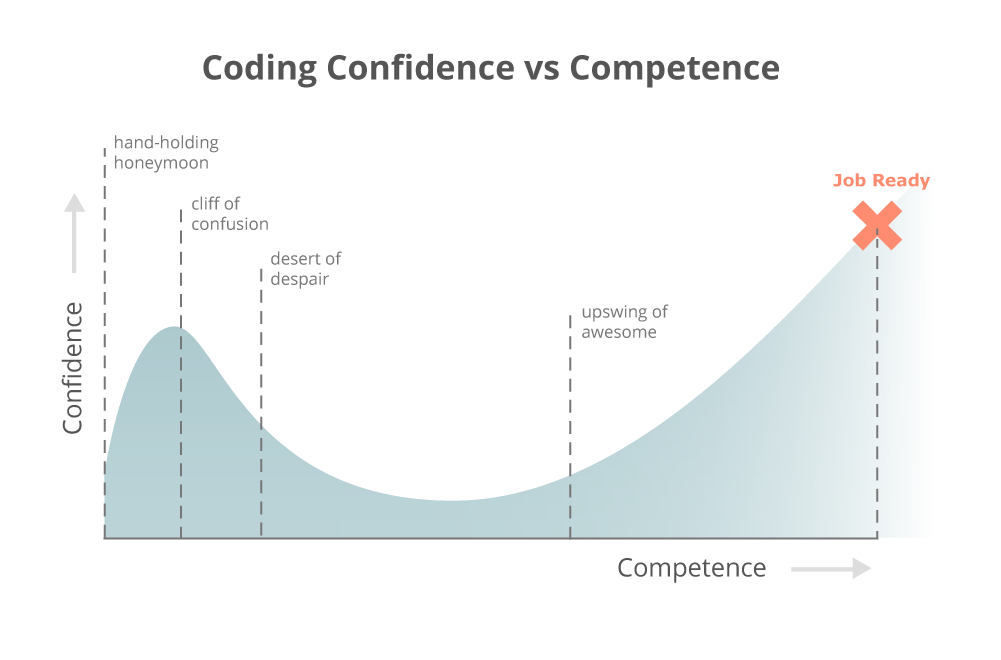
\includegraphics[width=0.95\linewidth,height=0.7\textheight,keepaspectratio]{coding_is_hard_confidence_competence} \end{center}

(图例``编程信心与能力'':纵轴为信心值,横轴为能力水平,虚线从左至右依次分割出手牵手蜜月期、混沌悬崖、绝望沙漠、令人兴奋的上升期四个阶段,第5条虚线标志着工作准备就绪)

\begin{itemize}
\item
  读文档是蜜月期,读读就过去,谁都会。
\item
  写程序是混沌悬崖,知道是这么回事,就是写不出来;
\item
  调程序是绝望沙漠,怎么看自己写的都对,就是编译器不开眼;
\item
  程序正确了就是兴奋期,万里长征迈出又一步。
\end{itemize}

\subsubsection{如何安装Python}\label{python}

Python社区有很多功能很好的包,但逐个安装需要解决繁杂的依赖关系。通常我会推荐安装已经做好的集成包,一劳永逸的解决后续问题。\href{https://store.continuum.io/cshop/anaconda/}{Anaconda}是最优先推荐的分发包,集成了常用的数值计算、图形处理、可视化等工具包如\texttt{IPython},
\texttt{matplotlib}, \texttt{numpy}, \texttt{scipy},
而且设定了更简单的安装Python模块的方法,可以节省大量的安装时间。

\paragraph{Python 常用包}\label{python-}

\begin{enumerate}
\def\labelenumi{\arabic{enumi}.}
\tightlist
\item
  科学计算 \texttt{Numpy}, \texttt{SciPy}
  (也是安装python包的拦路虎直到有了\href{http://mp.weixin.qq.com/s/A4_j8ZbyprMr1TT_wgisQQ}{conda})
\item
  类比于R的数据框操作包
  \href{http://mp.weixin.qq.com/s/1h-_J2NKjD1KyymPAeHPOg}{Pandas}
\item
  可视化工具 \texttt{Seaborn} (配合pandas), \texttt{matplotlib}
  (类比MATLAB), \texttt{plotly} (交互式绘图), \texttt{ggplot}
  (类比ggplot2)
\item
  网站开发 \texttt{web.py}, \texttt{Django}, \texttt{Flask}
\item
  任务调度和流程管理 \texttt{Airflow} (pipeline首选)
\item
  机器学习 \texttt{scikit-learn} (经典), \texttt{PyML},
  \texttt{Tensorflow} (谷歌释放), \texttt{pylearn2}, \texttt{Orange}
  (图形界面的机器学习包)
\item
  网页抓取 \texttt{Beautiful\ Soup},\texttt{requests},
\item
  可重复编程 \texttt{Jupyter}
\item
  正则表达式 \texttt{re}
\end{enumerate}

\subsubsection{如何运行Python命令和脚本}\label{python}

\begin{itemize}
\tightlist
\item
  对于初学者,本手册推荐直接在\texttt{Jupyter\ Notebook}下学习\texttt{Python}命令和脚本。我们这套教程也是用\texttt{Jupyter\ Notebook}写作而成,里面的代码可以随时修改和运行,并能同时记录你的脚本和输出,符合现在流行的``可重复性计算''的概念。

  \begin{itemize}
  \item
    Linux/Unix用户直接在终端(Terminal)进入你的目标文件夹\texttt{cd\ /working\_dir}{[}回车{]},然后在终端输入\texttt{Jupyter\ notebook}{[}回车{]}即可启动\texttt{Jupyter\ notebook}。
  \item
    Windows用户可以新建一个\texttt{Jupyter\_notebook.bat}文件(新建一个txt文件,写入内容后修改后缀为\texttt{.bat}。若不能修改后缀,请Google搜索``Window是如何显示文件扩展名''),并写入以下内容(注意把前两行的\emph{盘符}和\emph{路径}替换为你的工作目录),双击即可运行。

\begin{verbatim}
D:
cd PBR_training
jupyter notebook
pause
\end{verbatim}
  \item
    \texttt{Jupyter\ notebook}启动后会打开默认的浏览器(需要在图形用户界面下工作),这时可以\texttt{新建}或\texttt{打开}相应路径下的ipynb文件。
  \end{itemize}
\item
  对于LInux或Unix用户,直接在终端输入 \texttt{python}
  然后回车即可打开交互式\texttt{python}解释器,如下图所示。在这个解释器了敲入任何合法的\texttt{python}语句即可执行。此外,所有的命令还可以存储到一个文件一起执行,如下图所示。我们有一个包含\texttt{python}程序的文件\texttt{test.py},我们只要在终端输入\texttt{python\ test.py}并回车就可以运行这个文件。同时我们也可在终端通过输入\texttt{chmod\ 755\ test.py}赋予程序\texttt{test.py}可执行权限,并在终端输入\texttt{./test.py}运行\texttt{Python}脚本。更多Linux下的高级使用和Linux命令使用请见教程Bash\_training-chinese.ipynb。
\end{itemize}

\begin{center}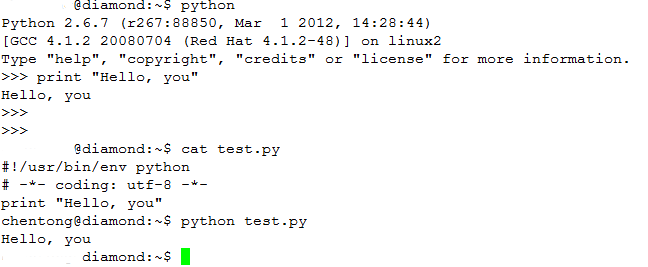
\includegraphics[width=0.95\linewidth,height=0.7\textheight,keepaspectratio]{Python_start_run_linux} \end{center}

\begin{itemize}
\item
  对于Windows用户,可以通过``Windows键+R''调出``Run''窗口并输入``cmd''打开Windows命令解释器,输入\texttt{python}即可打开交互式\texttt{python}解释器。同时也可以双击安装后的软件的快捷方式打开图形界面的\texttt{Python}解释器,可以处理交互式命令和导入Python文件并执行。
\item
  对于交互式\texttt{Python}解释器,在使用结束后,通过键盘组合键\texttt{Ctrl-d}
  (Linux/Unix)或\texttt{Ctrl-z} (Windows)关闭。
\end{itemize}

\subsubsection{使用什么编辑器写Python脚本}\label{python}

在你学成之后,可能主要操作都在服务器完成,而且日常工作一般会以脚本的形式解决。我个人推荐使用\href{http://www.vim.org/download.php}{Vim}来写作Python脚本。

Linux下\texttt{vim}的配置文件可从\href{https://github.com/Tong-Chen/vim}{我的
github}下载,Windows版可从\href{http://pan.baidu.com/s/1kT5KIN1}{我的百度云}
下载。

\subsection{Python程序事例}\label{python}

\begin{Shaded}
\begin{Highlighting}[]
\CommentTok{## 假如我们有如下FASTA格式的文件,我们想把多行序列合并为一行,怎么做?}
\ControlFlowTok{for} \NormalTok{line }\OperatorTok{in} \BuiltInTok{open}\NormalTok{(}\StringTok{"data/test2.fa"}\NormalTok{):}
    \BuiltInTok{print}\NormalTok{(line.strip())}
\end{Highlighting}
\end{Shaded}

\begin{verbatim}
>NM_001011874 gene=Xkr4 CDS=151-2091
gcggcggcgggcgagcgggcgctggagtaggagctggggagcggcgcggccggggaaggaagccagggcg
aggcgaggaggtggcgggaggaggagacagcagggacaggTGTCAGATAAAGGAGTGCTCTCCTCCGCTG
CCGAGGCATCATGGCCGCTAAGTCAGACGGGAGGCTGAAGATGAAGAAGAGCAGCGACGTGGCGTTCACC
CCGCTGCAGAACTCGGACAATTCGGGCTCTGTGCAAGGACTGGCTCCAGGCTTGCCGTCGGGGTCCGGAG
>NM_001195662 gene=Rp1 CDS=55-909
AAGCTCAGCCTTTGCTCAGATTCTCCTCTTGATGAAACAAAGGGATTTCTGCACATGCTTGAGAAATTGC
AGGTCTCACCCAAAATGAGTGACACACCTTCTACTAGTTTCTCCATGATTCATCTGACTTCTGAAGGTCA
AGTTCCTTCCCCTCGCCATTCAAATATCACTCATCCTGTAGTGGCTAAACGCATCAGTTTCTATAAGAGT
GGAGACCCACAGTTTGGCGGCGTTCGGGTGGTGGTCAACCCTCGTTCCTTTAAGACTTTTGACGCTCTGC
TGGACAGTTTATCCAGGAAGGTACCCCTGCCCTTTGGGGTAAGGAACATCAGCACGCCCCGTGGACGACA
CAGCATCACCAGGCTGGAGGAGCTAGAGGACGGCAAGTCTTATGTGTGCTCCCACAATAAGAAGGTGCTG
>NM_011283 gene=Rp1 CDS=128-6412
AATAAATCCAAAGACATTTGTTTACGTGAAACAAGCAGGTTGCATATCCAGTGACGTTTATACAGACCAC
ACAAACTATTTACTCTTTTCTTCGTAAGGAAAGGTTCAACTTCTGGTCTCACCCAAAATGAGTGACACAC
CTTCTACTAGTTTCTCCATGATTCATCTGACTTCTGAAGGTCAAGTTCCTTCCCCTCGCCATTCAAATAT
CACTCATCCTGTAGTGGCTAAACGCATCAGTTTCTATAAGAGTGGAGACCCACAGTTTGGCGGCGTTCGG
GTGGTGGTCAACCCTCGTTCCTTTAAGACTTTTGACGCTCTGCTGGACAGTTTATCCAGGAAGGTACCCC
TGCCCTTTGGGGTAAGGAACATCAGCACGCCCCGTGGACGACACAGCATCACCAGGCTGGAGGAGCTAGA
GGACGGCAAGTCTTATGTGTGCTCCCACAATAAGAAGGTGCTGCCAGTTGACCTGGACAAGGCCCGCAGG
CGCCCTCGGCCCTGGCTGAGTAGTCGCTCCATAAGCACGCATGTGCAGCTCTGTCCTGCAACTGCCAATA
TGTCCACCATGGCACCTGGCATGCTCCGTGCCCCAAGGAGGCTCGTGGTCTTCCGGAATGGTGACCCGAA
>NM_0112835 gene=Rp1 CDS=128-6412
AATAAATCCAAAGACATTTGTTTACGTGAAACAAGCAGGTTGCATATCCAGTGACGTTTATACAGACCAC
ACAAACTATTTACTCTTTTCTTCGTAAGGAAAGGTTCAACTTCTGGTCTCACCCAAAATGAGTGACACAC
CTTCTACTAGTTTCTCCATGATTCATCTGACTTCTGAAGGTCAAGTTCCTTCCCCTCGCCATTCAAATAT
CACTCATCCTGTAGTGGCTAAACGCATCAGTTTCTATAAGAGTGGAGACCCACAGTTTGGCGGCGTTCGG
GTGGTGGTCAACCCTCGTTCCTTTAAGACTTTTGACGCTCTGCTGGACAGTTTATCCAGGAAGGTACCCC
TGCCCTTTGGGGTAAGGAACATCAGCACGCCCCGTGGACGACACAGCATCACCAGGCTGGAGGAGCTAGA
GGACGGCAAGTCTTATGTGTGCTCCCACAATAAGAAGGTGCTGCCAGTTGACCTGGACAAGGCCCGCAGG
CGCCCTCGGCCCTGGCTGAGTAGTCGCTCCATAAGCACGCATGTGCAGCTCTGTCCTGCAACTGCCAATA
TGTCCACCATGGCACCTGGCATGCTCCGTGCCCCAAGGAGGCTCGTGGTCTTCCGGAATGGTGACCCGAA
\end{verbatim}

\begin{Shaded}
\begin{Highlighting}[]
\NormalTok{aDict }\OperatorTok{=} \NormalTok{\{\}}
\ControlFlowTok{for} \NormalTok{line }\OperatorTok{in} \BuiltInTok{open}\NormalTok{(}\StringTok{'data/test2.fa'}\NormalTok{):}
    \ControlFlowTok{if} \NormalTok{line[}\DecValTok{0}\NormalTok{] }\OperatorTok{==} \StringTok{'>'}\NormalTok{:}
        \NormalTok{key }\OperatorTok{=} \NormalTok{line.strip()}
        \NormalTok{aDict[key] }\OperatorTok{=} \NormalTok{[]}
    \ControlFlowTok{else}\NormalTok{:}
        \NormalTok{aDict[key].append(line.strip())}
\CommentTok{##------------------------------------------}
\ControlFlowTok{for} \NormalTok{key, valueL }\OperatorTok{in} \BuiltInTok{list}\NormalTok{(aDict.items()):}
    \BuiltInTok{print}\NormalTok{(key)}
    \BuiltInTok{print}\NormalTok{(}\StringTok{''}\NormalTok{.join(valueL))}
\end{Highlighting}
\end{Shaded}

\begin{verbatim}
>NM_001011874 gene=Xkr4 CDS=151-2091
gcggcggcgggcgagcgggcgctggagtaggagctggggagcggcgcggccggggaaggaagccagggcgaggcgaggaggtggcgggaggaggagacagcagggacaggTGTCAGATAAAGGAGTGCTCTCCTCCGCTGCCGAGGCATCATGGCCGCTAAGTCAGACGGGAGGCTGAAGATGAAGAAGAGCAGCGACGTGGCGTTCACCCCGCTGCAGAACTCGGACAATTCGGGCTCTGTGCAAGGACTGGCTCCAGGCTTGCCGTCGGGGTCCGGAG
>NM_001195662 gene=Rp1 CDS=55-909
AAGCTCAGCCTTTGCTCAGATTCTCCTCTTGATGAAACAAAGGGATTTCTGCACATGCTTGAGAAATTGCAGGTCTCACCCAAAATGAGTGACACACCTTCTACTAGTTTCTCCATGATTCATCTGACTTCTGAAGGTCAAGTTCCTTCCCCTCGCCATTCAAATATCACTCATCCTGTAGTGGCTAAACGCATCAGTTTCTATAAGAGTGGAGACCCACAGTTTGGCGGCGTTCGGGTGGTGGTCAACCCTCGTTCCTTTAAGACTTTTGACGCTCTGCTGGACAGTTTATCCAGGAAGGTACCCCTGCCCTTTGGGGTAAGGAACATCAGCACGCCCCGTGGACGACACAGCATCACCAGGCTGGAGGAGCTAGAGGACGGCAAGTCTTATGTGTGCTCCCACAATAAGAAGGTGCTG
>NM_011283 gene=Rp1 CDS=128-6412
AATAAATCCAAAGACATTTGTTTACGTGAAACAAGCAGGTTGCATATCCAGTGACGTTTATACAGACCACACAAACTATTTACTCTTTTCTTCGTAAGGAAAGGTTCAACTTCTGGTCTCACCCAAAATGAGTGACACACCTTCTACTAGTTTCTCCATGATTCATCTGACTTCTGAAGGTCAAGTTCCTTCCCCTCGCCATTCAAATATCACTCATCCTGTAGTGGCTAAACGCATCAGTTTCTATAAGAGTGGAGACCCACAGTTTGGCGGCGTTCGGGTGGTGGTCAACCCTCGTTCCTTTAAGACTTTTGACGCTCTGCTGGACAGTTTATCCAGGAAGGTACCCCTGCCCTTTGGGGTAAGGAACATCAGCACGCCCCGTGGACGACACAGCATCACCAGGCTGGAGGAGCTAGAGGACGGCAAGTCTTATGTGTGCTCCCACAATAAGAAGGTGCTGCCAGTTGACCTGGACAAGGCCCGCAGGCGCCCTCGGCCCTGGCTGAGTAGTCGCTCCATAAGCACGCATGTGCAGCTCTGTCCTGCAACTGCCAATATGTCCACCATGGCACCTGGCATGCTCCGTGCCCCAAGGAGGCTCGTGGTCTTCCGGAATGGTGACCCGAA
>NM_0112835 gene=Rp1 CDS=128-6412
AATAAATCCAAAGACATTTGTTTACGTGAAACAAGCAGGTTGCATATCCAGTGACGTTTATACAGACCACACAAACTATTTACTCTTTTCTTCGTAAGGAAAGGTTCAACTTCTGGTCTCACCCAAAATGAGTGACACACCTTCTACTAGTTTCTCCATGATTCATCTGACTTCTGAAGGTCAAGTTCCTTCCCCTCGCCATTCAAATATCACTCATCCTGTAGTGGCTAAACGCATCAGTTTCTATAAGAGTGGAGACCCACAGTTTGGCGGCGTTCGGGTGGTGGTCAACCCTCGTTCCTTTAAGACTTTTGACGCTCTGCTGGACAGTTTATCCAGGAAGGTACCCCTGCCCTTTGGGGTAAGGAACATCAGCACGCCCCGTGGACGACACAGCATCACCAGGCTGGAGGAGCTAGAGGACGGCAAGTCTTATGTGTGCTCCCACAATAAGAAGGTGCTGCCAGTTGACCTGGACAAGGCCCGCAGGCGCCCTCGGCCCTGGCTGAGTAGTCGCTCCATAAGCACGCATGTGCAGCTCTGTCCTGCAACTGCCAATATGTCCACCATGGCACCTGGCATGCTCCGTGCCCCAAGGAGGCTCGTGGTCTTCCGGAATGGTGACCCGAA
\end{verbatim}

\subsection{Python语法}\label{python}

\subsubsection{层级缩进}

\begin{itemize}
\tightlist
\item
  合适的缩进。空白在Python中是很重要的,它称为缩进。在逻辑行首的空白(空格和制表符)用来决定逻辑行的缩进层次,从而用来决定语句的分组。这意味着同一层次的语句必须有相同的缩进。每一组这样的语句称为一个块。通常的缩进为4个空格,
  在\texttt{Jupyter\ Notebook}中为一个\texttt{Tab}键。
\end{itemize}

从下面这两个例子可以看出错误的缩进类型和对应的提示。 * ``unexpected
indent'' 表示在不该出现空白的地方多了空白,并且指出问题出在第三行(line
3)。 * ``expected an indented block''
表示应该有缩进的地方未缩进,也指出了问题所在行。 * ``unindent does not
match any outer indentation level''
表示缩进出现了不一致,问题通常会在指定行\textbf{及其前面的行}。

\begin{Shaded}
\begin{Highlighting}[]
\BuiltInTok{print}\NormalTok{(}\StringTok{"不合适的缩进会引发错误,b前不该有的缩进"}\NormalTok{)}
\NormalTok{a }\OperatorTok{=} \StringTok{'No indent'}
 \NormalTok{b }\OperatorTok{=} \StringTok{'我前面有个空格……'}
\end{Highlighting}
\end{Shaded}

\begin{verbatim}
  File "<ipython-input-2-ff110daefedf>", line 3
    b = '我前面有个空格……'
    ^
IndentationError: unexpected indent
\end{verbatim}

\begin{Shaded}
\begin{Highlighting}[]
\BuiltInTok{print}\NormalTok{(}\StringTok{"不合适的缩进,print是for的子语句,应该有缩进,却漏掉了"}\NormalTok{)}
\NormalTok{a }\OperatorTok{=} \NormalTok{[}\DecValTok{1}\NormalTok{,}\DecValTok{2}\NormalTok{,}\DecValTok{3}\NormalTok{]}

\ControlFlowTok{for} \NormalTok{i }\OperatorTok{in} \NormalTok{a:}
\BuiltInTok{print} \StringTok{"我应该被缩进,我从属于for循环!!!}\CharTok{\textbackslash{}n}\StringTok{"}
\end{Highlighting}
\end{Shaded}

\begin{verbatim}
  File "<ipython-input-3-84bbc644895e>", line 5
    print "我应该被缩进,我从属于for循环!!!\n"
        ^
IndentationError: expected an indented block
\end{verbatim}

\begin{Shaded}
\begin{Highlighting}[]
\NormalTok{a }\OperatorTok{=} \NormalTok{[}\DecValTok{1}\NormalTok{,}\DecValTok{2}\NormalTok{, }\DecValTok{3}\NormalTok{]}
\ControlFlowTok{if} \NormalTok{a:}
    \ControlFlowTok{for} \NormalTok{i }\OperatorTok{in} \NormalTok{a:}
        \BuiltInTok{print}\NormalTok{(i)}
       \BuiltInTok{print}\NormalTok{(i }\OperatorTok{+} \DecValTok{1}\NormalTok{, }
             \StringTok{"为什么我的缩进跟其它行不一样呢,我的空格被谁吃了?"}\NormalTok{)}
         \BuiltInTok{print}\NormalTok{(i }\OperatorTok{+} \DecValTok{1}\NormalTok{, }
               \StringTok{"为什么我的缩进跟其它行不一样呢,谁给了我个空格?"}\NormalTok{)}
\end{Highlighting}
\end{Shaded}

\begin{verbatim}
  File "<tokenize>", line 5
    print(i + 1,
    ^
IndentationError: unindent does not match any outer indentation level
\end{verbatim}

\subsubsection{Python作为计算器的使用}\label{python}

Python中可以进行基本的数学运算,与小学中学过的一样,加减乘除取余数等,需要注意的是运算符的优先级。

\begin{Shaded}
\begin{Highlighting}[]
\DecValTok{2} \OperatorTok{+} \DecValTok{2}
\end{Highlighting}
\end{Shaded}

\begin{verbatim}
4
\end{verbatim}

\begin{Shaded}
\begin{Highlighting}[]
\DecValTok{2} \OperatorTok{+} \DecValTok{3} \OperatorTok{+}\DecValTok{5}
\end{Highlighting}
\end{Shaded}

\begin{verbatim}
10
\end{verbatim}

\begin{Shaded}
\begin{Highlighting}[]
\DecValTok{2} \OperatorTok{+} \DecValTok{3} \OperatorTok{*} \DecValTok{5} 
\end{Highlighting}
\end{Shaded}

\begin{verbatim}
17
\end{verbatim}

\begin{Shaded}
\begin{Highlighting}[]
\NormalTok{(}\DecValTok{2} \OperatorTok{+} \DecValTok{3}\NormalTok{) }\OperatorTok{*} \DecValTok{5}
\end{Highlighting}
\end{Shaded}

\begin{verbatim}
25
\end{verbatim}

\begin{Shaded}
\begin{Highlighting}[]
\CommentTok{## 整除}
\DecValTok{23} \OperatorTok{//} \DecValTok{7}
\end{Highlighting}
\end{Shaded}

\begin{verbatim}
3
\end{verbatim}

\begin{Shaded}
\begin{Highlighting}[]
\CommentTok{## 取余数}
\DecValTok{23} \OperatorTok{%} \DecValTok{7}
\end{Highlighting}
\end{Shaded}

\begin{verbatim}
2
\end{verbatim}

\paragraph{第一个小程序}

\begin{Shaded}
\begin{Highlighting}[]
\BuiltInTok{print}\NormalTok{(}\StringTok{"Hello, Python!"}\NormalTok{)}
\end{Highlighting}
\end{Shaded}

\begin{verbatim}
Hello, Python!
\end{verbatim}

\begin{Shaded}
\begin{Highlighting}[]
\NormalTok{myname }\OperatorTok{=} \BuiltInTok{input}\NormalTok{(}\StringTok{"Your name: "}\NormalTok{)}
\BuiltInTok{print}\NormalTok{(}\StringTok{"Hello"}\NormalTok{, myname)}
\end{Highlighting}
\end{Shaded}

\begin{verbatim}
Your name: CT
Hello CT
\end{verbatim}

\subsubsection{变量、数据结构、流程控制}

我们先看一个动图展示内存中变量的赋值、存储、值的改变和程序的运行。

点击访问动图 \url{http://www.ehbio.com/ehbio_resource/python_tutor.gif}

\begin{itemize}
\item
  常量,指固定的数字或字符串,如\texttt{2}, \texttt{2.9},
  \texttt{"Hello\ world"}等。
\item
  变量,存储了数字或字符串的事物称为变量,它可以被赋值或被修改。简单的可以理解为变量是一个盒子,你可以把任何东西放在里面,通过盒子的名字来取出盒子内的东西。

  \begin{itemize}
  \tightlist
  \item
    数值变量:存储了数的变量。\\
  \item
    字符串变量:存储了字符串的变量。字符串变量的名字最好不为\texttt{str},可以使用\texttt{aStr}。
  \item
    列表 (list):
    list是处理一组\emph{有序}项目的数据结构,即你可以在一个列表中存储一个
    \emph{序列}
    的项目。假想你有一个购物列表,上面记载着你要买的东西,你就容易理解列表了。只不过在你的购物表上,可能每样东西都独自占有一行,而在Python中,你在每个项目之间用逗号分割。列表中的项目应该包括在\textbf{方括号}中,这样Python就知道你是在指明一个列表。一旦你创建了一个列表,你可以添加、删除或是搜索列表中的项目。由于你可以增加或删除项目,我们说列表是
    \emph{可变的}
    数据类型,即这种类型是可以被改变的。列表变量的名字最好不为\texttt{list},可以使用\texttt{aList}。
  \item
    元祖
    (tuple):元组和列表十分类似,但是不可修改。元组通过\textbf{圆括号中用逗号分割的项目}定义。元组通常用在使语句或用户定义的函数能够安全地采用一组值的时候,即被使用的元组的值不会改变。元组变量的名字最好不为\texttt{tuple},可以使用\texttt{aTuple}。
  \item
    集合
    (Set):也与列表类似,但是元素不可重复。通常用来去除重复、求交集、并集等。而且集合的查询速度远远快于列表,可以用来提高运算速度。
  \item
    字典 (dict):
    字典类似于你通过联系人名字查找地址和联系人详细情况的地址簿,即,我们把键(名字)和值(详细情况)联系在一起。注意,键必须是唯一的,就像如果有两个人恰巧同名的话,你无法找到正确的信息。多个键可以指向同一个值。当一个键需要指向多个值时,这些值需要放在列表、元组或字典里面。注意,你只能使用不可变的对象(字符串,数字,元组)来作为字典的键,但是可以用不可变或可变的对象作为字典的值。键值对在字典中以这样的方式标记:d
    = \{key1 : value1, key2 : value2
    \}。注意它们的键/值对用冒号分割,而各个对用逗号分割,所有这些都包括在\textbf{花括号}中。记住字典中的键/值对是没有顺序的。如果你想要一个特定的顺序,那么你应该在使用前自己对它们排序。列表变量的名字最好不为\texttt{dict},可以使用\texttt{aDict}。
  \item
    序列:列表、元组、字符串都是一种序列格式。同时还可以使用range来产生序列。序列的两个主要操作时\emph{索引操作}和\emph{切片操作}。
  \end{itemize}
\item
  标示符

  \begin{itemize}
  \tightlist
  \item
    变量的名字被称为标示符。标识符对大小写敏感,第一个字符必须是字母表中的字母(大写或小写)或者一个下划线(\_),其它部分额外包含数字。有效的标示符有:
    \texttt{abc}, \texttt{\_abc}, \texttt{a\_b\_2},
    \texttt{\_\_23}等。无效的标示符有: \texttt{2a}, \texttt{3b}。
  \item
    标示符最好不使用Python内置的关键字,如\texttt{str}, \texttt{list},
    \texttt{int}, \texttt{def}, \texttt{split}, \texttt{dict}等。
  \item
    标示符最好能言词达意,即展示变量的类型,又带有变量的实际含义。如\texttt{line}表示文件的一行,\texttt{lineL}表示存有从文件读入的每一行的列表。
  \end{itemize}
\item
  控制流

  \begin{itemize}
  \tightlist
  \item
    \texttt{if}语句
  \end{itemize}

  \texttt{if}语句用来检验一个条件,如果条件为真,我们运行一块语句(称为
  \texttt{if-块}),否则我们处理另外一块语句(称为
  \texttt{else-块})。\texttt{else}
  从句是可选的。如果有多个条件,中间使用\texttt{elif}。

  举个例子:``买五个包子,如果看到卖西瓜的,买一个''------最后程序猿买了一个包子''
  \texttt{买包子\ =\ 5\ \ \ if\ 看到卖西瓜的:\ \ \ \ \ \ \ 买包子\ =\ 1}

  \begin{itemize}
  \tightlist
  \item
    \texttt{For}语句
  \end{itemize}

  for..in是一个循环语句,它在一序列的对象上递归,即逐一使用队列中的每个项目。

  \begin{itemize}
  \tightlist
  \item
    \texttt{While}语句
  \end{itemize}

  只要在一个条件为真的情况下,\texttt{while}语句允许你重复执行一块语句。\texttt{while}语句是所谓
  \emph{循环}
  语句的一个例子。\texttt{while}语句有一个可选的\texttt{else}从句。

  \begin{itemize}
  \tightlist
  \item
    \texttt{break}语句是用来 \emph{终止}
    循环语句的,即哪怕循环条件没有成为False或序列还没有被完全递归,也停止执行循环语句。
  \end{itemize}

  一个重要的注释是,如果你从\texttt{for}或\texttt{while}循环中
  \emph{终止} ,任何对应的循环else块将不执行。

  \begin{itemize}
  \item
    \texttt{continue}语句被用来告诉\texttt{Python}跳过当前循环块中的剩余语句,然后
    \emph{继续} 进行下一轮循环。
  \item
    逻辑运算符 \texttt{and}, \texttt{or}, \texttt{not}。
  \end{itemize}
\end{itemize}

\begin{Shaded}
\begin{Highlighting}[]
\CommentTok{## 变量名命名:为清晰表达,驼峰式,下划线式}
\NormalTok{LookLikeThis }\OperatorTok{=} \DecValTok{1}
\NormalTok{look_like_this }\OperatorTok{=} \StringTok{'a'}
\end{Highlighting}
\end{Shaded}

\paragraph{Python中的数据类型:整数(int)、浮点(float)和字符串(str)}\label{pythonintfloatstr-1}

\begin{Shaded}
\begin{Highlighting}[]
\BuiltInTok{type}\NormalTok{(}\DecValTok{2}\NormalTok{)}
\end{Highlighting}
\end{Shaded}

\begin{verbatim}
int
\end{verbatim}

\begin{Shaded}
\begin{Highlighting}[]
\BuiltInTok{type}\NormalTok{(}\FloatTok{2.5}\NormalTok{)}
\end{Highlighting}
\end{Shaded}

\begin{verbatim}
float
\end{verbatim}

\begin{Shaded}
\begin{Highlighting}[]
\BuiltInTok{type}\NormalTok{(}\StringTok{"Hello, everyone"}\NormalTok{)}
\end{Highlighting}
\end{Shaded}

\begin{verbatim}
str
\end{verbatim}

\begin{Shaded}
\begin{Highlighting}[]
\BuiltInTok{type}\NormalTok{([}\DecValTok{1}\NormalTok{,}\DecValTok{2}\NormalTok{,}\DecValTok{3}\NormalTok{])}
\end{Highlighting}
\end{Shaded}

\begin{verbatim}
list
\end{verbatim}

\begin{Shaded}
\begin{Highlighting}[]
\CommentTok{## 类型转换函数}
\BuiltInTok{str}\NormalTok{()}
\BuiltInTok{int}\NormalTok{()}
\BuiltInTok{float}\NormalTok{()}
\end{Highlighting}
\end{Shaded}

\begin{Shaded}
\begin{Highlighting}[]
\BuiltInTok{str}\NormalTok{(}\DecValTok{2}\NormalTok{)}
\end{Highlighting}
\end{Shaded}

\begin{verbatim}
'2'
\end{verbatim}

\begin{Shaded}
\begin{Highlighting}[]
\CommentTok{## 字符和数字不同}
\DecValTok{42} \OperatorTok{!=} \StringTok{"42"}
\end{Highlighting}
\end{Shaded}

\begin{verbatim}
True
\end{verbatim}

\begin{Shaded}
\begin{Highlighting}[]
\DecValTok{42} \OperatorTok{==} \BuiltInTok{int}\NormalTok{(}\StringTok{"42"}\NormalTok{)}
\end{Highlighting}
\end{Shaded}

\begin{verbatim}
True
\end{verbatim}

\begin{Shaded}
\begin{Highlighting}[]
\CommentTok{## This is my first python program!}

\NormalTok{myName }\OperatorTok{=} \BuiltInTok{input}\NormalTok{(}\StringTok{"Hello, what is your name?"}\NormalTok{)}
\BuiltInTok{print}\NormalTok{(}\StringTok{'It is  good to meet you,'} \OperatorTok{+} \NormalTok{myName)}
\BuiltInTok{print}\NormalTok{(}\StringTok{'The length of your name is'}\NormalTok{, }\BuiltInTok{str}\NormalTok{(}\BuiltInTok{len}\NormalTok{(myName)))}

\NormalTok{myAge }\OperatorTok{=} \BuiltInTok{input}\NormalTok{(}\StringTok{'What is your age?'}\NormalTok{)}
\BuiltInTok{print}\NormalTok{(}\StringTok{'You will be '} \OperatorTok{+} \BuiltInTok{str}\NormalTok{(}\BuiltInTok{int}\NormalTok{(myAge) }\OperatorTok{+} \DecValTok{1}\NormalTok{) }\OperatorTok{+} \StringTok{' in a year.'}\NormalTok{)}
\end{Highlighting}
\end{Shaded}

\begin{verbatim}
Hello, what is your name?CT
It is  good to meet you,CT
The length of your name is 2
What is your age?20
You will be 21 in a year.
\end{verbatim}

\paragraph{逻辑值和比较操作}

\begin{Shaded}
\begin{Highlighting}[]
\NormalTok{a }\OperatorTok{=} \VariableTok{False}
\NormalTok{a}
\end{Highlighting}
\end{Shaded}

\begin{verbatim}
False
\end{verbatim}

\begin{Shaded}
\begin{Highlighting}[]
\NormalTok{b }\OperatorTok{=} \VariableTok{True}
\NormalTok{b}
\end{Highlighting}
\end{Shaded}

\begin{verbatim}
True
\end{verbatim}

\begin{Shaded}
\begin{Highlighting}[]
\NormalTok{a }\OperatorTok{=} \StringTok{"False"}
\NormalTok{a}
\end{Highlighting}
\end{Shaded}

\begin{verbatim}
'False'
\end{verbatim}

\begin{Shaded}
\begin{Highlighting}[]
\DecValTok{42} \OperatorTok{==} \DecValTok{40}
\end{Highlighting}
\end{Shaded}

\begin{verbatim}
False
\end{verbatim}

\begin{Shaded}
\begin{Highlighting}[]
\DecValTok{42} \OperatorTok{==} \StringTok{"42"}
\end{Highlighting}
\end{Shaded}

\begin{verbatim}
False
\end{verbatim}

\begin{Shaded}
\begin{Highlighting}[]
\DecValTok{30} \OperatorTok{==} \DecValTok{30}
\end{Highlighting}
\end{Shaded}

\begin{verbatim}
True
\end{verbatim}

\begin{Shaded}
\begin{Highlighting}[]
\CommentTok{## 注意赋值(一个=)和比较(==)的区别}
\NormalTok{a }\OperatorTok{=} \StringTok{'hello'}

\NormalTok{a }\OperatorTok{==} \StringTok{'hello'}
\end{Highlighting}
\end{Shaded}

\begin{verbatim}
True
\end{verbatim}

\subparagraph{\texorpdfstring{布尔操作符\texttt{and}, \texttt{or},
\texttt{not}}{布尔操作符and, or, not}}\label{and-or-not}

\begin{itemize}
\tightlist
\item
  逻辑与 \texttt{and}:所有为真才为真
\item
  逻辑或 \texttt{or}:所有为假才为假
\item
  逻辑非 \texttt{not}: 真变假,假变真
\end{itemize}

\begin{Shaded}
\begin{Highlighting}[]
\NormalTok{(}\DecValTok{3} \OperatorTok{>} \DecValTok{2}\NormalTok{) }\OperatorTok{and} \NormalTok{(}\DecValTok{5} \OperatorTok{<} \DecValTok{6}\NormalTok{)}
\end{Highlighting}
\end{Shaded}

\begin{verbatim}
True
\end{verbatim}

\begin{Shaded}
\begin{Highlighting}[]
\NormalTok{(}\DecValTok{3} \OperatorTok{<} \DecValTok{2}\NormalTok{) }\OperatorTok{or} \NormalTok{(}\DecValTok{5} \OperatorTok{<} \DecValTok{6}\NormalTok{)}
\end{Highlighting}
\end{Shaded}

\begin{verbatim}
True
\end{verbatim}

\begin{Shaded}
\begin{Highlighting}[]
\OperatorTok{not} \VariableTok{True}
\end{Highlighting}
\end{Shaded}

\begin{verbatim}
False
\end{verbatim}

\paragraph{控制流}\label{-1}

if 条件(True or False) :

\begin{verbatim}
代码块1
\end{verbatim}

elif 条件 :

\begin{verbatim}
代码块
\end{verbatim}

else :

\begin{verbatim}
代码块2
\end{verbatim}

\begin{Shaded}
\begin{Highlighting}[]
\CommentTok{##条件}
\NormalTok{name }\OperatorTok{=} \BuiltInTok{input}\NormalTok{(}\StringTok{'Please enter a name and click Enter}\CharTok{\textbackslash{}n}\StringTok{'}\NormalTok{)}
\ControlFlowTok{if} \NormalTok{name }\OperatorTok{==} \StringTok{'ehbio'}\NormalTok{:}
    \BuiltInTok{print} \NormalTok{(}\StringTok{'hello ehbio'}\NormalTok{)}
\ControlFlowTok{else} \NormalTok{:}
    \BuiltInTok{print} \NormalTok{(}\StringTok{'You are not ehbio'}\NormalTok{)}
\end{Highlighting}
\end{Shaded}

\begin{verbatim}
Please enter a name and click Enter
CT
You are not ehbio
\end{verbatim}

\paragraph{While循环}\label{while-1}

\begin{Shaded}
\begin{Highlighting}[]
\NormalTok{a }\OperatorTok{=} \DecValTok{0}
\ControlFlowTok{while} \NormalTok{a }\OperatorTok{<} \DecValTok{5}\NormalTok{:}
    \BuiltInTok{print}\NormalTok{(}\StringTok{'Hello, world'}\NormalTok{)}
    \NormalTok{a }\OperatorTok{=} \NormalTok{a }\OperatorTok{+} \DecValTok{1}
\end{Highlighting}
\end{Shaded}

\begin{verbatim}
Hello, world
Hello, world
Hello, world
Hello, world
Hello, world
\end{verbatim}

\paragraph{数值变量操作}

\begin{Shaded}
\begin{Highlighting}[]
\BuiltInTok{print}\NormalTok{(}\StringTok{"数值变量"}\NormalTok{)}
\NormalTok{a }\OperatorTok{=} \DecValTok{5}   \CommentTok{#注意等号两边的空格,为了易于辨识,操作符两侧最好有空格,数量不限}
\BuiltInTok{print}\NormalTok{(a)}

\BuiltInTok{print}\NormalTok{()}
\BuiltInTok{print}\NormalTok{(}\StringTok{"The type of a is"}\NormalTok{, }\BuiltInTok{type}\NormalTok{(a))}

\CommentTok{##print "这是保留节目,通常判断变量的类型使用的不是type是isinstance."}
\CommentTok{##print "a is an int, ", isinstance(a,int)}

\CommentTok{## 再次赋值就是覆盖}
\NormalTok{a }\OperatorTok{=} \DecValTok{6}
\BuiltInTok{print}\NormalTok{(a)}
\end{Highlighting}
\end{Shaded}

\begin{verbatim}
数值变量
5

The type of a is <class 'int'>
6
\end{verbatim}

\begin{Shaded}
\begin{Highlighting}[]
\CommentTok{## 判断}
\BuiltInTok{print}\NormalTok{(}\StringTok{"比较数值的大小"}\NormalTok{)}
\NormalTok{a }\OperatorTok{=} \DecValTok{5}

\CommentTok{## 注意大于号两边的空格,为了易于辨识,操作符两侧最好有空格,数量不限}
\ControlFlowTok{if} \NormalTok{a }\OperatorTok{>} \DecValTok{4}\NormalTok{:}
    \BuiltInTok{print}\NormalTok{(}\StringTok{"a is larger than 4."}\NormalTok{)}
\ControlFlowTok{elif} \NormalTok{a }\OperatorTok{==} \DecValTok{4}\NormalTok{:}
    \BuiltInTok{print}\NormalTok{(}\StringTok{"a is equal to 4."}\NormalTok{)}
\ControlFlowTok{else}\NormalTok{:}
    \BuiltInTok{print}\NormalTok{(}\StringTok{"a is less than 4"}\NormalTok{)}
\end{Highlighting}
\end{Shaded}

\begin{verbatim}
比较数值的大小
a is larger than 4.
\end{verbatim}

\begin{Shaded}
\begin{Highlighting}[]
\BuiltInTok{print}\NormalTok{(}\StringTok{"给定数值变量a和b的值,通过判断和重新赋值使得a的值小,b的值大"}\NormalTok{)}
\NormalTok{a }\OperatorTok{=} \DecValTok{5}
\NormalTok{b }\OperatorTok{=} \DecValTok{3}

\ControlFlowTok{if} \NormalTok{a }\OperatorTok{>} \NormalTok{b:}
    \NormalTok{a,b }\OperatorTok{=} \NormalTok{b,a}
\CommentTok{##-------------------}
\BuiltInTok{print}\NormalTok{(a)}
\BuiltInTok{print}\NormalTok{(b)}
\end{Highlighting}
\end{Shaded}

\begin{verbatim}
给定数值变量a和b的值,通过判断和重新赋值使得a的值小,b的值大
3
5
\end{verbatim}

\begin{Shaded}
\begin{Highlighting}[]
\BuiltInTok{print}\NormalTok{(}\StringTok{'''#数值运算, 符合传统的优先级,需要使用括号来改变优先级,}
\StringTok{和小学学的数学一模一样!!'''}\NormalTok{)}
\NormalTok{a }\OperatorTok{=} \DecValTok{5}
\NormalTok{b }\OperatorTok{=} \DecValTok{3}

\BuiltInTok{print}\NormalTok{(}\StringTok{"a + b ="}\NormalTok{, a }\OperatorTok{+} \NormalTok{b)}
\BuiltInTok{print}\NormalTok{(}\StringTok{"a * b ="}\NormalTok{, a }\OperatorTok{*} \NormalTok{b)}
\BuiltInTok{print}\NormalTok{(}\StringTok{"a / b ="}\NormalTok{, a }\OperatorTok{/} \NormalTok{b)  }\CommentTok{# 1}
\BuiltInTok{print}\NormalTok{(}\StringTok{"2 * (a+b) ="}\NormalTok{, }\DecValTok{2} \OperatorTok{*} \NormalTok{(a }\OperatorTok{+} \NormalTok{b))}
\BuiltInTok{print}\NormalTok{(}\StringTok{"取余数: a % b ="}\NormalTok{, a }\OperatorTok{%} \NormalTok{b)}
\BuiltInTok{print}\NormalTok{(}\StringTok{"取余数是很好的判断循环的地方,因为每个固定的周期余数就会循环一次"}\NormalTok{)}
\end{Highlighting}
\end{Shaded}

\begin{verbatim}
#数值运算, 符合传统的优先级,需要使用括号来改变优先级,
和小学学的数学一模一样!!
a + b = 8
a * b = 15
a / b = 1.6666666666666667
2 * (a+b) = 16
取余数: a % b = 2
取余数是很好的判断循环的地方,因为每个固定的周期余数就会循环一次
\end{verbatim}

\begin{Shaded}
\begin{Highlighting}[]
\DecValTok{3} \OperatorTok{/} \DecValTok{0}
\end{Highlighting}
\end{Shaded}

\begin{verbatim}
---------------------------------------------------------------------------

ZeroDivisionError                         Traceback (most recent call last)

<ipython-input-17-2b706ee9dd8e> in <module>()
----> 1 3 / 0


ZeroDivisionError: division by zero
\end{verbatim}

\paragraph{字符串变量操作}

\begin{Shaded}
\begin{Highlighting}[]
\BuiltInTok{print}\NormalTok{(}\StringTok{"字符串变量"}\NormalTok{)}

\CommentTok{## 注意引号的配对}
\NormalTok{a }\OperatorTok{=} \StringTok{"Hello, welcome to Python"}

\CommentTok{##a = 123}
\CommentTok{##a = str(a)}

\BuiltInTok{print}\NormalTok{(}\StringTok{"The string a is:"}\NormalTok{, a)}
\BuiltInTok{print}\NormalTok{()}

\CommentTok{## 占位符}
\BuiltInTok{print}\NormalTok{(}\StringTok{"The length of this string <}\SpecialCharTok{%s}\StringTok{> is }\SpecialCharTok \NormalTok{(a, }\BuiltInTok{len}\NormalTok{(a)))}
\BuiltInTok{print}\NormalTok{()}

\BuiltInTok{print}\NormalTok{(}\StringTok{"The type of a is"}\NormalTok{, }\BuiltInTok{type}\NormalTok{(a))}
\end{Highlighting}
\end{Shaded}

\begin{verbatim}
字符串变量
The string a is: Hello, welcome to Python

The length of this string <Hello, welcome to Python> is 24

The type of a is <class 'str'>
\end{verbatim}

\begin{Shaded}
\begin{Highlighting}[]
\NormalTok{a }\OperatorTok{=} \StringTok{"大事赖独断而不赖众谋"}
\BuiltInTok{print}\NormalTok{(}\StringTok{"The string a is:"}\NormalTok{, a)}
\BuiltInTok{print}\NormalTok{()}

\CommentTok{## len函数:获得字符串长度}
\BuiltInTok{print}\NormalTok{(}\StringTok{"The length of this string <}\SpecialCharTok{%s}\StringTok{> is }\SpecialCharTok \NormalTok{(a, }\BuiltInTok{len}\NormalTok{(a)))}
\BuiltInTok{print}\NormalTok{()}
\end{Highlighting}
\end{Shaded}

\begin{verbatim}
The string a is: 大事赖独断而不赖众谋

The length of this string <大事赖独断而不赖众谋> is 10
\end{verbatim}

\begin{Shaded}
\begin{Highlighting}[]
\NormalTok{a }\OperatorTok{=} \StringTok{"Hello, welcome to Python"}

\BuiltInTok{print}\NormalTok{(}\StringTok{"取出字符串的第一个字符、最后一个字符、中间部分字符"}\NormalTok{)}
\BuiltInTok{print}\NormalTok{(}\StringTok{"The first character of a is }\SpecialCharTok \NormalTok{a[}\DecValTok{0}\NormalTok{])}

\BuiltInTok{print}\NormalTok{(}\StringTok{"The first five characters of a are }\SpecialCharTok \NormalTok{a[}\DecValTok{0}\NormalTok{:}\DecValTok{5}\NormalTok{])}

\BuiltInTok{print}\NormalTok{(}\StringTok{"The last character of a is }\SpecialCharTok \NormalTok{a[}\OperatorTok{-}\DecValTok{1}\NormalTok{])}
\BuiltInTok{print}\NormalTok{(}\StringTok{"The last two characters of a are }\SpecialCharTok \NormalTok{a[}\OperatorTok{-}\DecValTok{2}\NormalTok{:])}
\BuiltInTok{print}\NormalTok{(}\StringTok{"The last character of a is }\SpecialCharTok \NormalTok{a[}\BuiltInTok{len}\NormalTok{(a) }\OperatorTok{-} \DecValTok{1}\NormalTok{])}
\BuiltInTok{print}\NormalTok{(}\StringTok{"}\CharTok{\textbackslash{}n}\StringTok{这部分很重要啊,字符串的索引和切片操作是及其常用的。"}\NormalTok{)}
\end{Highlighting}
\end{Shaded}

\begin{verbatim}
取出字符串的第一个字符、最后一个字符、中间部分字符
The first character of a is H

The first five characters of a are Hello

The last character of a is n

The last two characters of a are on

The last character of a is n


这部分很重要啊,字符串的索引和切片操作是及其常用的。
\end{verbatim}

\begin{Shaded}
\begin{Highlighting}[]
\NormalTok{a }\OperatorTok{=} \StringTok{"oaoaoaoa"}

\BuiltInTok{print}\NormalTok{(}\StringTok{"遍历字符串"}\NormalTok{)}
\ControlFlowTok{for} \NormalTok{i }\OperatorTok{in} \NormalTok{a:}
    \BuiltInTok{print}\NormalTok{(i)}

\BuiltInTok{print}\NormalTok{()}
\BuiltInTok{print}\NormalTok{(}\StringTok{"The index of first <o> is: "}\NormalTok{,a.find(}\StringTok{'o'}\NormalTok{))}
\BuiltInTok{print}\NormalTok{(}\StringTok{"The index of first <c> is: "}\NormalTok{,a.find(}\StringTok{'c'}\NormalTok{))}
    
\BuiltInTok{print}\NormalTok{(}\StringTok{"输出符合特定要求的字符的位置"}\NormalTok{)}
\BuiltInTok{print}\NormalTok{()}
\NormalTok{pos }\OperatorTok{=} \DecValTok{0}
\ControlFlowTok{for} \NormalTok{i }\OperatorTok{in} \NormalTok{a:}
    \NormalTok{pos }\OperatorTok{+=} \DecValTok{1}
    \ControlFlowTok{if} \NormalTok{i }\OperatorTok{==} \StringTok{'o'}\NormalTok{:}
        \BuiltInTok{print}\NormalTok{(pos)}
    \CommentTok{#-------------------}
\CommentTok{##-----------------------}
\BuiltInTok{print}\NormalTok{(}\StringTok{'''}\CharTok{\textbackslash{}n}\StringTok{知道吗?不经意间我们写出了Python的}
\StringTok{一个内置的标准函数find或者index,而且功能还更强大'''}\NormalTok{)}

\BuiltInTok{print}\NormalTok{(}\StringTok{'''}\CharTok{\textbackslash{}n}\StringTok{自己尝试实现程序语言内建的函数是学习程序语言}
\StringTok{的很好方法。'''}\NormalTok{)}
\end{Highlighting}
\end{Shaded}

\begin{verbatim}
遍历字符串
o
a
o
a
o
a
o
a

The index of first <o> is:  0
The index of first <c> is:  -1
输出符合特定要求的字符的位置

1
3
5
7

知道吗?不经意间我们写出了Python的
一个内置的标准函数find或者index,而且功能还更强大

自己尝试实现程序语言内建的函数是学习程序语言
的很好方法。
\end{verbatim}

\begin{Shaded}
\begin{Highlighting}[]
\BuiltInTok{print}\NormalTok{(}\StringTok{"我们看看用内置函数如何找到所有 o 的位置}\CharTok{\textbackslash{}n}\StringTok{"}\NormalTok{)}
\NormalTok{a }\OperatorTok{=} \StringTok{"oaoaoaoa"}

\BuiltInTok{print}\NormalTok{(}\StringTok{"内置函数find只能确定最先出现的 o 的位置"}\NormalTok{)}
\NormalTok{pos }\OperatorTok{=} \NormalTok{a.find(}\StringTok{'o'}\NormalTok{)}

\BuiltInTok{print}\NormalTok{(}\StringTok{"因此,我们要在发现 o 之后,截取其后的字符串,再执行find操作"}\NormalTok{)}
\ControlFlowTok{while} \DecValTok{1}\NormalTok{:}
    \BuiltInTok{print}\NormalTok{(pos }\OperatorTok{+} \DecValTok{1}\NormalTok{)}
    \NormalTok{new }\OperatorTok{=} \NormalTok{a[pos }\OperatorTok{+} \DecValTok{1}\NormalTok{:].find(}\StringTok{'o'}\NormalTok{)}
    \ControlFlowTok{if} \NormalTok{new }\OperatorTok{==} \OperatorTok{-}\DecValTok{1}\NormalTok{:}
        \ControlFlowTok{break}
    \NormalTok{pos }\OperatorTok{=} \NormalTok{new }\OperatorTok{+} \NormalTok{pos }\OperatorTok{+} \DecValTok{1}
\CommentTok{## help(str)}
\end{Highlighting}
\end{Shaded}

\begin{verbatim}
我们看看用内置函数如何找到所有 o 的位置

内置函数find只能确定最先出现的 o 的位置
因此,我们要在发现 o 之后,截取其后的字符串,再执行find操作
1
3
5
7
\end{verbatim}

\begin{Shaded}
\begin{Highlighting}[]
\BuiltInTok{print}\NormalTok{()}
\BuiltInTok{print}\NormalTok{(}\StringTok{"利用split分割字符串}\CharTok{\textbackslash{}n}\StringTok{"}\NormalTok{)}
\NormalTok{str1 }\OperatorTok{=} \StringTok{"a b c d e f g"}
\NormalTok{strL }\OperatorTok{=} \NormalTok{str1.split(}\StringTok{' '}\NormalTok{)}
\BuiltInTok{print}\NormalTok{(strL)}
\BuiltInTok{print}\NormalTok{(}\StringTok{"}\CharTok{\textbackslash{}n}\StringTok{使用split命令就可以把字符串分成列表了,想取用哪一列都随便你了。"}\NormalTok{)}
\CommentTok{## 使用下面的命令查看可以对字符串进行的操作}
\CommentTok{## help(str)}
\end{Highlighting}
\end{Shaded}

\begin{verbatim}
利用split分割字符串

['a', 'b', 'c', 'd', 'e', 'f', 'g']

使用split命令就可以把字符串分成列表了,想取用哪一列都随便你了。
\end{verbatim}

\begin{Shaded}
\begin{Highlighting}[]
\BuiltInTok{print}\NormalTok{(}\StringTok{"字符串的连接}\CharTok{\textbackslash{}n}\StringTok{"}\NormalTok{)}

\NormalTok{a }\OperatorTok{=} \StringTok{"Hello"}
\NormalTok{b }\OperatorTok{=} \StringTok{"Python"}
\NormalTok{c }\OperatorTok{=} \NormalTok{a }\OperatorTok{+} \StringTok{', '} \OperatorTok{+} \NormalTok{b}
\BuiltInTok{print}\NormalTok{(c)}
\BuiltInTok{print}\NormalTok{(}\StringTok{"}\CharTok{\textbackslash{}n}\StringTok{原来字符串相加就可以连起来啊!}\CharTok{\textbackslash{}n}\StringTok{"}\NormalTok{)}
\BuiltInTok{print}\NormalTok{(}\StringTok{'''注意,这不是连接字符串最好的方式。}
\StringTok{考虑到字符串是不可修改的,每次连接操作都是新开辟一个内存空间,}
\StringTok{把字符串存到里面,这样的连接操作执行几十万次会很影响运行速度。'''}\NormalTok{)}
\end{Highlighting}
\end{Shaded}

\begin{verbatim}
字符串的连接

Hello, Python

原来字符串相加就可以连起来啊!

注意,这不是连接字符串最好的方式。
考虑到字符串是不可修改的,每次连接操作都是新开辟一个内存空间,
把字符串存到里面,这样的连接操作执行几十万次会很影响运行速度。
\end{verbatim}

关于字符串链接为什么不推荐使用
\texttt{+},文章\href{https://mp.weixin.qq.com/s/n5kkZfC8FGlzeBODarLHcw}{为啥我的Python这么慢
(一)}给出了一个很好的演示例子。

\begin{Shaded}
\begin{Highlighting}[]
\BuiltInTok{print}\NormalTok{(}\StringTok{'''去除字符串中特定的字符。通常我们在文件中读取的一行都包含换行符,}
\StringTok{linux下为}\CharTok{\textbackslash{}\textbackslash{}}\StringTok{n }\CharTok{\textbackslash{}n}\StringTok{'''}\NormalTok{)  }\CommentTok{# \textbackslash{}\textbackslash{}转义字符}

\NormalTok{a }\OperatorTok{=} \StringTok{"oneline}\CharTok{\textbackslash{}n}\StringTok{"}
\BuiltInTok{print}\NormalTok{(}\StringTok{"Currently, the string <a> is **"}\NormalTok{, a, }\StringTok{"**. \textbackslash{}}
\CharTok{\textbackslash{}n}\StringTok{ The length of string <a> is **"}\NormalTok{, }\BuiltInTok{len}\NormalTok{(a), }\StringTok{"**. \textbackslash{}}
\CharTok{\textbackslash{}n}\StringTok{ 我为什么换到下一行了?}\CharTok{\textbackslash{}n}\StringTok{"}\NormalTok{)}

\NormalTok{a }\OperatorTok{=} \NormalTok{a.strip()}
\BuiltInTok{print}\NormalTok{(}\StringTok{"Currently, the string <a> is **"}\NormalTok{, a, }\StringTok{"**. \textbackslash{}}
\CharTok{\textbackslash{}n}\StringTok{ The length of string <a> is **"}\NormalTok{, }\BuiltInTok{len}\NormalTok{(a), }\StringTok{"**. \textbackslash{}}
\CharTok{\textbackslash{}n}\StringTok{ 删掉了换行符后,少了个字符,而且没换行!}\CharTok{\textbackslash{}n}\StringTok{"}\NormalTok{)}

\NormalTok{a }\OperatorTok{=} \NormalTok{a.strip(}\StringTok{'o'}\NormalTok{)}
\BuiltInTok{print}\NormalTok{(}\StringTok{"Currently, the string <a> is **"}\NormalTok{, a, }\StringTok{"**. \textbackslash{}}
\CharTok{\textbackslash{}n}\StringTok{ The length of string <a> is **"}\NormalTok{, }\BuiltInTok{len}\NormalTok{(a), }\StringTok{"**. \textbackslash{}}
\StringTok{又少了个字符!!}\CharTok{\textbackslash{}n}\StringTok{"}\NormalTok{)}

\NormalTok{a }\OperatorTok{=} \NormalTok{a.strip(}\StringTok{'one'}\NormalTok{)}
\BuiltInTok{print}\NormalTok{(}\StringTok{"Currently, the string <a> is **"}\NormalTok{, a, }\StringTok{"**. \textbackslash{}}
\CharTok{\textbackslash{}n}\StringTok{ The length of string <a> is **"}\NormalTok{, }\BuiltInTok{len}\NormalTok{(a), }\StringTok{"**. \textbackslash{}}
\StringTok{又少字符了!!}\CharTok{\textbackslash{}n}\StringTok{"}\NormalTok{)}
\end{Highlighting}
\end{Shaded}

\begin{verbatim}
去除字符串中特定的字符。通常我们在文件中读取的一行都包含换行符,
linux下为\n 

Currently, the string <a> is ** oneline
 **. 
 The length of string <a> is ** 8 **. 
 我为什么换到下一行了?

Currently, the string <a> is ** oneline **. 
 The length of string <a> is ** 7 **. 
 删掉了换行符后,少了个字符,而且没换行!

Currently, the string <a> is ** neline **. 
 The length of string <a> is ** 6 **. 又少了个字符!!

Currently, the string <a> is ** li **. 
 The length of string <a> is ** 2 **. 又少字符了!!
\end{verbatim}

\begin{Shaded}
\begin{Highlighting}[]
\BuiltInTok{print}\NormalTok{(}\StringTok{"字符串的替换}\CharTok{\textbackslash{}n}\StringTok{"}\NormalTok{)}

\NormalTok{a }\OperatorTok{=} \StringTok{"Hello, Python"}
\NormalTok{b }\OperatorTok{=} \NormalTok{a.replace(}\StringTok{"Hello"}\NormalTok{, }\StringTok{"Welcome"}\NormalTok{)}
\BuiltInTok{print}\NormalTok{(}\StringTok{"原始字符串是:"}\NormalTok{, a)}
\BuiltInTok{print}\NormalTok{()}
\BuiltInTok{print}\NormalTok{(}\StringTok{"替换后的字符串是:"}\NormalTok{, b)}
\BuiltInTok{print}\NormalTok{()}

\NormalTok{c }\OperatorTok{=} \NormalTok{a.replace(}\StringTok{"o"}\NormalTok{, }\StringTok{"O"}\NormalTok{)}
\BuiltInTok{print}\NormalTok{(c)}
\BuiltInTok{print}\NormalTok{(}\StringTok{"所有的o都被替换了!}\CharTok{\textbackslash{}n}\StringTok{"}\NormalTok{)}

\BuiltInTok{print}\NormalTok{(}\StringTok{"如果我只替换第一个o怎么办呢?}\CharTok{\textbackslash{}n}\StringTok{"}\NormalTok{)}
\NormalTok{c }\OperatorTok{=} \NormalTok{a.replace(}\StringTok{"o"}\NormalTok{, }\StringTok{"O"}\NormalTok{, }\DecValTok{1}\NormalTok{)}
\BuiltInTok{print}\NormalTok{(c)}
\end{Highlighting}
\end{Shaded}

\begin{verbatim}
字符串的替换

原始字符串是: Hello, Python

替换后的字符串是: Welcome, Python

HellO, PythOn
所有的o都被替换了!

如果我只替换第一个o怎么办呢?

HellO, Python
\end{verbatim}

\begin{Shaded}
\begin{Highlighting}[]
\CommentTok{## 中文替换也可以}
\NormalTok{a }\OperatorTok{=} \StringTok{"忙处事为,常向闲中先检点,过举自稀;动时念想,预从静里密操持,非心自息。"}
\BuiltInTok{print}\NormalTok{(a.replace(}\StringTok{';'}\NormalTok{, }\StringTok{'}\CharTok{\textbackslash{}n}\StringTok{'}\NormalTok{))}
\end{Highlighting}
\end{Shaded}

\begin{verbatim}
忙处事为,常向闲中先检点,过举自稀
动时念想,预从静里密操持,非心自息。
\end{verbatim}

\begin{Shaded}
\begin{Highlighting}[]
\BuiltInTok{print}\NormalTok{(}\StringTok{"字符串帮助,查看字符串可用方法"}\NormalTok{)}
\BuiltInTok{help}\NormalTok{(}\BuiltInTok{str}\NormalTok{)}
\end{Highlighting}
\end{Shaded}

\begin{Shaded}
\begin{Highlighting}[]
\BuiltInTok{print}\NormalTok{(}\StringTok{"大小写判断和转换"}\NormalTok{)}
\NormalTok{a }\OperatorTok{=} \StringTok{'Sdsdsd'}
\BuiltInTok{print}\NormalTok{(}\StringTok{"All elements in <}\SpecialCharTok{%s}\StringTok{> is lowercase: }\SpecialCharTok \NormalTok{(a, a.islower()))}
\BuiltInTok{print}\NormalTok{(}\StringTok{"Transfer all elments in <}\SpecialCharTok{%s}\StringTok{> to lowerse <}\SpecialCharTok \NormalTok{(a, a.lower()))}
\BuiltInTok{print}\NormalTok{(}\StringTok{"Transfer all elments in <}\SpecialCharTok{%s}\StringTok{> to upperse <}\SpecialCharTok \NormalTok{(a, a.upper()))}
\end{Highlighting}
\end{Shaded}

\begin{verbatim}
大小写判断和转换
All elements in <Sdsdsd> is lowercase: False
Transfer all elments in <Sdsdsd> to lowerse <sdsdsd>
Transfer all elments in <Sdsdsd> to upperse <SDSDSD>
\end{verbatim}

\begin{Shaded}
\begin{Highlighting}[]
\BuiltInTok{print}\NormalTok{(}\StringTok{"这个是个保留节目,有兴趣的看,无兴趣的跳过不影响学习"}\NormalTok{)}
\BuiltInTok{print}\NormalTok{(}\StringTok{'''字符串是不可修改的,}
\StringTok{同一个变量名字赋不同的只实际是产生了多个不同的变量。}
\StringTok{不同的变量名字赋同样的值,用于比较时相等,但引用不同的区域'''}\NormalTok{)}


\NormalTok{b }\OperatorTok{=} \StringTok{"123456"}
\CommentTok{## print b}
\BuiltInTok{print}\NormalTok{(}\StringTok{"The memory index of b is"}\NormalTok{, }\BuiltInTok{id}\NormalTok{(b))}
\ControlFlowTok{for} \NormalTok{i }\OperatorTok{in} \BuiltInTok{range}\NormalTok{(}\DecValTok{1}\NormalTok{, }\DecValTok{15}\NormalTok{, }\DecValTok{2}\NormalTok{):}
    \NormalTok{b }\OperatorTok{=} \NormalTok{b }\OperatorTok{+} \StringTok{'123456'}
    \CommentTok{# print b}
    \BuiltInTok{print}\NormalTok{(}\StringTok{"The memory index of b is"}\NormalTok{, }\BuiltInTok{id}\NormalTok{(b))}
\end{Highlighting}
\end{Shaded}

\begin{verbatim}
这个是个保留节目,有兴趣的看,无兴趣的跳过不影响学习
字符串是不可修改的,
同一个变量名字赋不同的只实际是产生了多个不同的变量。
不同的变量名字赋同样的值,用于比较时相等,但引用不同的区域
The memory index of b is 139844870936200
The memory index of b is 139844868463728
The memory index of b is 139844870954056
The memory index of b is 139844863857088
The memory index of b is 139844863857088
The memory index of b is 139845221506544
The memory index of b is 139844869671408
The memory index of b is 139844868660840
\end{verbatim}

\begin{Shaded}
\begin{Highlighting}[]
\BuiltInTok{print}\NormalTok{(}\StringTok{"字符串转数组"}\NormalTok{)}
\BuiltInTok{print}\NormalTok{()}
\NormalTok{str1 }\OperatorTok{=} \StringTok{"ACTG"}
\BuiltInTok{print}\NormalTok{(}\BuiltInTok{list}\NormalTok{(str1))}
\NormalTok{a }\OperatorTok{=} \BuiltInTok{list}\NormalTok{(str1)}

\BuiltInTok{print}\NormalTok{()}
\BuiltInTok{print}\NormalTok{(}\StringTok{"字符串转数组之后就可以逆序了,得到其反向序列"}\NormalTok{)}
\BuiltInTok{print}\NormalTok{()}
\NormalTok{a.reverse()}
\BuiltInTok{print}\NormalTok{(}\StringTok{''}\NormalTok{.join(a))}
\end{Highlighting}
\end{Shaded}

\begin{verbatim}
字符串转数组

['A', 'C', 'T', 'G']

字符串转数组之后就可以逆序了,得到其反向序列

GTCA
\end{verbatim}

\begin{Shaded}
\begin{Highlighting}[]
\BuiltInTok{print}\NormalTok{(}\StringTok{"数字字符串转数值"}\NormalTok{)}
\NormalTok{a }\OperatorTok{=} \StringTok{'123'}
\BuiltInTok{print}\NormalTok{(a }\OperatorTok{+} \StringTok{'1'}\NormalTok{, }\BuiltInTok{int}\NormalTok{(a) }\OperatorTok{+} \DecValTok{1}\NormalTok{)}
\NormalTok{a }\OperatorTok{=} \StringTok{'123.5'}

\BuiltInTok{print}\NormalTok{()}
\CommentTok{## print a + 1}
\BuiltInTok{print}\NormalTok{(}\BuiltInTok{float}\NormalTok{(a) }\OperatorTok{+} \DecValTok{1}\NormalTok{)}
\BuiltInTok{print}\NormalTok{(}\StringTok{'''从文件或命令行参数中取出的数字都是字符串形式出现,}
\StringTok{做四则运算时要先用int 或 float转换。'''}\NormalTok{)}
\end{Highlighting}
\end{Shaded}

\begin{verbatim}
数字字符串转数值
1231 124

124.5
从文件或命令行参数中取出的数字都是字符串形式出现,
做四则运算时要先用int 或 float转换。
\end{verbatim}

\begin{Shaded}
\begin{Highlighting}[]
\BuiltInTok{print}\NormalTok{(}\StringTok{"字符串倍增"}\NormalTok{)}
\NormalTok{a }\OperatorTok{=} \StringTok{"ehbio "}
\NormalTok{a }\OperatorTok{*} \DecValTok{4}
\end{Highlighting}
\end{Shaded}

\begin{verbatim}
字符串倍增





'ehbio ehbio ehbio ehbio '
\end{verbatim}

\begin{Shaded}
\begin{Highlighting}[]
\NormalTok{a }\OperatorTok{*} \DecValTok{0}
\end{Highlighting}
\end{Shaded}

\begin{verbatim}
''
\end{verbatim}

\begin{Shaded}
\begin{Highlighting}[]
\CommentTok{## 倍增不可以是小数}
\NormalTok{a }\OperatorTok{*} \FloatTok{3.1}
\end{Highlighting}
\end{Shaded}

\begin{verbatim}
---------------------------------------------------------------------------

TypeError                                 Traceback (most recent call last)

<ipython-input-21-c65dd4dac397> in <module>()
----> 1 a * 3.1


TypeError: can't multiply sequence by non-int of type 'float'
\end{verbatim}

\paragraph{break和continue}\label{breakcontinue-1}

\begin{Shaded}
\begin{Highlighting}[]
\CommentTok{## 模拟登陆账号, 用户名 Bob, 密码fish}
\ControlFlowTok{while} \VariableTok{True}\NormalTok{:}
    \NormalTok{name }\OperatorTok{=} \BuiltInTok{input}\NormalTok{(}\StringTok{'Who are you?}\CharTok{\textbackslash{}n}\StringTok{> '}\NormalTok{)}
    \ControlFlowTok{if} \NormalTok{name }\OperatorTok{!=} \StringTok{'Bob'}\NormalTok{:}
        \ControlFlowTok{continue}  \CommentTok{# 将程序跳转到开头}
    \NormalTok{password }\OperatorTok{=} \BuiltInTok{input}\NormalTok{(}\StringTok{'Hello, Bob. What is your password? (password: fish)}\CharTok{\textbackslash{}n}\StringTok{> '}\NormalTok{)}
    \ControlFlowTok{if} \NormalTok{password }\OperatorTok{==} \StringTok{'fish'}\NormalTok{:}
        \ControlFlowTok{break} \CommentTok{# 跳出所在循环或最内层循环}
\BuiltInTok{print}\NormalTok{(}\StringTok{'Acess granted!'}\NormalTok{)}
\end{Highlighting}
\end{Shaded}

\begin{verbatim}
Who are you?
> CT
Who are you?
> Bob
Hello, Bob. What is your password? (password: fish)
> sdsds
Who are you?
> Bob
Hello, Bob. What is your password? (password: fish)
> fish
Acess granted!
\end{verbatim}

\paragraph{for range (获取一系列数)}\label{for-range-}

\begin{Shaded}
\begin{Highlighting}[]
\CommentTok{## 如果只给一个参数,则是从0-给定参数(不包括),步长为1}
\ControlFlowTok{for} \NormalTok{i }\OperatorTok{in} \BuiltInTok{range}\NormalTok{(}\DecValTok{4}\NormalTok{):}
    \BuiltInTok{print}\NormalTok{(i)}
\end{Highlighting}
\end{Shaded}

\begin{verbatim}
0
1
2
3
\end{verbatim}

\begin{Shaded}
\begin{Highlighting}[]
\CommentTok{## 1: start; 10: end (不包括); 2: step}
\ControlFlowTok{for} \NormalTok{i }\OperatorTok{in} \BuiltInTok{range}\NormalTok{(}\DecValTok{1}\NormalTok{,}\DecValTok{10}\NormalTok{,}\DecValTok{2}\NormalTok{):}
    \BuiltInTok{print}\NormalTok{(i)}
\end{Highlighting}
\end{Shaded}

\begin{verbatim}
1
3
5
7
9
\end{verbatim}

\begin{Shaded}
\begin{Highlighting}[]
\CommentTok{## 步长也可以为负值,从大到小}
\ControlFlowTok{for} \NormalTok{i }\OperatorTok{in} \BuiltInTok{range}\NormalTok{(}\DecValTok{10}\NormalTok{,}\DecValTok{1}\NormalTok{,}\OperatorTok{-}\DecValTok{2}\NormalTok{):}
    \BuiltInTok{print}\NormalTok{(i)}
\end{Highlighting}
\end{Shaded}

\begin{verbatim}
10
8
6
4
2
\end{verbatim}

高斯计算1-100的加和。

\begin{Shaded}
\begin{Highlighting}[]
\CommentTok{## 高斯的1+2+3+...+100=?}
\NormalTok{total }\OperatorTok{=} \DecValTok{0}

\CommentTok{## 参数是101,为什么呢?}
\ControlFlowTok{for} \NormalTok{i }\OperatorTok{in} \BuiltInTok{range}\NormalTok{(}\DecValTok{1}\NormalTok{,}\DecValTok{101}\NormalTok{):}
    \NormalTok{total }\OperatorTok{=} \NormalTok{total }\OperatorTok{+} \NormalTok{i}
\BuiltInTok{print}\NormalTok{(total)}
\end{Highlighting}
\end{Shaded}

\begin{verbatim}
5050
\end{verbatim}

\begin{Shaded}
\begin{Highlighting}[]
\CommentTok{## 高斯优化后的}
\NormalTok{end }\OperatorTok{=} \DecValTok{100}
\NormalTok{sum_all }\OperatorTok{=} \BuiltInTok{int}\NormalTok{((}\DecValTok{1}\OperatorTok{+}\NormalTok{end) }\OperatorTok{*} \NormalTok{end }\OperatorTok{/} \DecValTok{2}\NormalTok{)}
\CommentTok{##else:}
\CommentTok{##    sum_all = end * (end -1 ) / 2 + end}
\BuiltInTok{print}\NormalTok{(sum_all)}
\end{Highlighting}
\end{Shaded}

\begin{verbatim}
5050
\end{verbatim}

脑筋急转弯,题目如下:

现有100元钱,需要买100个物品,其中铅笔盒单价5元,笔单价3元,橡皮单价0.5元,怎么组合可以把100元花完,同时三种物品的个数和为100,请用编程解决。

\begin{Shaded}
\begin{Highlighting}[]
\CommentTok{## 纯暴力解法}
\ControlFlowTok{for} \NormalTok{x }\OperatorTok{in} \BuiltInTok{range}\NormalTok{(}\DecValTok{0}\NormalTok{, }\DecValTok{101}\NormalTok{):}
    \ControlFlowTok{for} \NormalTok{y }\OperatorTok{in} \BuiltInTok{range}\NormalTok{(}\DecValTok{0}\NormalTok{, }\DecValTok{101}\NormalTok{):}
        \ControlFlowTok{for} \NormalTok{z }\OperatorTok{in} \BuiltInTok{range}\NormalTok{(}\DecValTok{0}\NormalTok{, }\DecValTok{101}\NormalTok{):}
            \ControlFlowTok{if} \NormalTok{x }\OperatorTok{+} \NormalTok{y }\OperatorTok{+} \NormalTok{z }\OperatorTok{==} \DecValTok{100} \OperatorTok{and} \DecValTok{5} \OperatorTok{*} \NormalTok{x }\OperatorTok{+} \DecValTok{3} \OperatorTok{*} \NormalTok{y }\OperatorTok{+} \FloatTok{0.5} \OperatorTok{*} \NormalTok{z }\OperatorTok{==} \DecValTok{100}\NormalTok{:}
                \BuiltInTok{print}\NormalTok{(x, y, z)}
\end{Highlighting}
\end{Shaded}

\begin{verbatim}
0 20 80
5 11 84
10 2 88
\end{verbatim}

\begin{Shaded}
\begin{Highlighting}[]
\CommentTok{## 优化后的暴力解法}
\CommentTok{## 限定box和pen的最大数目,也就是全部钱只买他们,最多能买多少个?}
\NormalTok{max_box }\OperatorTok{=} \BuiltInTok{int}\NormalTok{(}\DecValTok{100} \OperatorTok{/} \DecValTok{5}\NormalTok{) }\OperatorTok{+} \DecValTok{1}
\NormalTok{max_pen }\OperatorTok{=} \BuiltInTok{int}\NormalTok{(}\DecValTok{100} \OperatorTok{/} \DecValTok{3}\NormalTok{) }\OperatorTok{+} \DecValTok{1}
\ControlFlowTok{for} \NormalTok{box_num }\OperatorTok{in} \BuiltInTok{range}\NormalTok{(max_box):}
    \CommentTok{# 需要买的物品总数是固定的,}
    \ControlFlowTok{for} \NormalTok{pen_num }\OperatorTok{in} \BuiltInTok{range}\NormalTok{(max_pen }\OperatorTok{-} \NormalTok{box_num):}
        \NormalTok{eraser_num }\OperatorTok{=} \DecValTok{100} \OperatorTok{-} \NormalTok{box_num }\OperatorTok{-} \NormalTok{pen_num}
        \ControlFlowTok{if} \DecValTok{5} \OperatorTok{*} \NormalTok{box_num }\OperatorTok{+} \DecValTok{3} \OperatorTok{*} \NormalTok{pen_num }\OperatorTok{+} \FloatTok{0.5} \OperatorTok{*} \NormalTok{eraser_num }\OperatorTok{==} \DecValTok{100}\NormalTok{:}
            \BuiltInTok{print}\NormalTok{((box_num, pen_num, eraser_num))}
\end{Highlighting}
\end{Shaded}

\begin{verbatim}
(0, 20, 80)
(5, 11, 84)
(10, 2, 88)
\end{verbatim}

\paragraph{列表操作}

\begin{Shaded}
\begin{Highlighting}[]
\BuiltInTok{print}\NormalTok{(}\StringTok{"#构建一个数组"}\NormalTok{)}
\NormalTok{aList }\OperatorTok{=} \NormalTok{[}\DecValTok{1}\NormalTok{, }\DecValTok{2}\NormalTok{, }\DecValTok{3}\NormalTok{, }\DecValTok{4}\NormalTok{, }\DecValTok{5}\NormalTok{]}
\BuiltInTok{print}\NormalTok{(aList)}
\BuiltInTok{print}\NormalTok{(}\StringTok{"}\CharTok{\textbackslash{}n}\StringTok{数组可以用下标或区域进行索引}\CharTok{\textbackslash{}n}\StringTok{"}\NormalTok{)}
\BuiltInTok{print}\NormalTok{(}\StringTok{"The first element is }\SpecialCharTok \NormalTok{aList[}\DecValTok{0}\NormalTok{])}
\BuiltInTok{print}\NormalTok{()}
\BuiltInTok{print}\NormalTok{(}\StringTok{"The last element is }\SpecialCharTok \NormalTok{aList[}\OperatorTok{-}\DecValTok{1}\NormalTok{])}
\BuiltInTok{print}\NormalTok{()}
\BuiltInTok{print}\NormalTok{(}\StringTok{"The first two elements are"}\NormalTok{, aList[:}\DecValTok{2}\NormalTok{])}
\BuiltInTok{print}\NormalTok{(}\StringTok{"}\CharTok{\textbackslash{}n}\StringTok{数组索引和切片操作与字符串是一样一样的,而且都很重要。"}\NormalTok{)}
\end{Highlighting}
\end{Shaded}

\begin{verbatim}
#构建一个数组
[1, 2, 3, 4, 5]

数组可以用下标或区域进行索引

The first element is 1.

The last element is 5.

The first two elements are [1, 2]

数组索引和切片操作与字符串是一样一样的,而且都很重要。
\end{verbatim}

\begin{Shaded}
\begin{Highlighting}[]
\NormalTok{aList }\OperatorTok{=} \NormalTok{[]}
\BuiltInTok{print}\NormalTok{(}\StringTok{"#append: 向数组中增加元素"}\NormalTok{)}
\NormalTok{aList.append(}\DecValTok{6}\NormalTok{)}
\BuiltInTok{print}\NormalTok{(aList)}

\BuiltInTok{print}\NormalTok{(}\StringTok{"}\CharTok{\textbackslash{}n}\StringTok{#extend: 向数组中增加一个数组"}\NormalTok{)}
\BuiltInTok{print}\NormalTok{()}
\NormalTok{bList }\OperatorTok{=} \NormalTok{[}\StringTok{'a'}\NormalTok{, }\StringTok{'b'}\NormalTok{, }\StringTok{'c'}\NormalTok{]}
\NormalTok{aList.extend(bList)}
\BuiltInTok{print}\NormalTok{(aList)}

\NormalTok{aList }\OperatorTok{+} \NormalTok{bList}
\end{Highlighting}
\end{Shaded}

\begin{verbatim}
#append: 向数组中增加元素
[6]

#extend: 向数组中增加一个数组

[6, 'a', 'b', 'c']





[6, 'a', 'b', 'c', 'a', 'b', 'c']
\end{verbatim}

\begin{Shaded}
\begin{Highlighting}[]
\NormalTok{aList }\OperatorTok{=} \NormalTok{[}\DecValTok{1}\NormalTok{, }\DecValTok{2}\NormalTok{, }\DecValTok{3}\NormalTok{, }\DecValTok{4}\NormalTok{, }\DecValTok{3}\NormalTok{, }\DecValTok{5}\NormalTok{]}
\BuiltInTok{print}\NormalTok{(}\StringTok{"在数组中删除元素"}\NormalTok{)}
\NormalTok{aList.remove(}\DecValTok{3}\NormalTok{)  }\CommentTok{# 只删除第一个匹配的 3}
\BuiltInTok{print}\NormalTok{()}
\BuiltInTok{print}\NormalTok{(aList)}

\NormalTok{aList.pop(}\DecValTok{3}\NormalTok{)  }\CommentTok{# 移除元素的下标为3的字符}
\BuiltInTok{print}\NormalTok{()}
\BuiltInTok{print}\NormalTok{(aList)}
\BuiltInTok{print}\NormalTok{(}\StringTok{'''}\CharTok{\textbackslash{}n}\StringTok{pop和remove是不一样的,remove是移除等于给定值的元素,}
\StringTok{pop是移除给定位置的元素}\CharTok{\textbackslash{}n}\StringTok{'''}\NormalTok{)}
\end{Highlighting}
\end{Shaded}

\begin{verbatim}
在数组中删除元素

[1, 2, 4, 3, 5]

[1, 2, 4, 5]

pop和remove是不一样的,remove是移除等于给定值的元素,
pop是移除给定位置的元素
\end{verbatim}

\begin{Shaded}
\begin{Highlighting}[]
\NormalTok{aList }\OperatorTok{=} \NormalTok{[}\DecValTok{1}\NormalTok{, }\DecValTok{2}\NormalTok{, }\DecValTok{3}\NormalTok{, }\DecValTok{4}\NormalTok{, }\DecValTok{5}\NormalTok{]}

\BuiltInTok{print}\NormalTok{(}\StringTok{"#遍历数组的每个元素"}\NormalTok{)}
\BuiltInTok{print}\NormalTok{()}
\ControlFlowTok{for} \NormalTok{ele }\OperatorTok{in} \NormalTok{aList:}
    \BuiltInTok{print}\NormalTok{(ele)}

\BuiltInTok{print}\NormalTok{(}\StringTok{"}\CharTok{\textbackslash{}n}\StringTok{#输出数组,并输出大于3的元素"}\NormalTok{)}
\BuiltInTok{print}\NormalTok{()}

\ControlFlowTok{for} \NormalTok{ele }\OperatorTok{in} \NormalTok{aList:}
    \ControlFlowTok{if} \NormalTok{ele }\OperatorTok{>} \DecValTok{3}\NormalTok{:}
        \BuiltInTok{print}\NormalTok{(ele)}
\end{Highlighting}
\end{Shaded}

\begin{verbatim}
#遍历数组的每个元素

1
2
3
4
5
#输出数组中大于3的元素

4
5
\end{verbatim}

\begin{Shaded}
\begin{Highlighting}[]
\NormalTok{aList }\OperatorTok{=} \NormalTok{[i }\ControlFlowTok{for} \NormalTok{i }\OperatorTok{in} \BuiltInTok{range}\NormalTok{(}\DecValTok{30}\NormalTok{)]}
\NormalTok{aList}
\NormalTok{aList }\OperatorTok{=} \NormalTok{[i }\ControlFlowTok{for} \NormalTok{i }\OperatorTok{in} \BuiltInTok{range}\NormalTok{(}\DecValTok{30}\NormalTok{) }\ControlFlowTok{if} \NormalTok{i }\OperatorTok{%} \DecValTok{2} \OperatorTok{==}\DecValTok{0}\NormalTok{]}
\NormalTok{aList}
\end{Highlighting}
\end{Shaded}

\begin{verbatim}
[0, 2, 4, 6, 8, 10, 12, 14, 16, 18, 20, 22, 24, 26, 28]
\end{verbatim}

\begin{Shaded}
\begin{Highlighting}[]
\NormalTok{aList }\OperatorTok{=} \NormalTok{[i }\ControlFlowTok{for} \NormalTok{i }\OperatorTok{in} \BuiltInTok{range}\NormalTok{(}\DecValTok{30}\NormalTok{)]}
\BuiltInTok{print}\NormalTok{(}\StringTok{"#输出数组中大于3,且小于10的元素"}\NormalTok{)}
\BuiltInTok{print}\NormalTok{()}

\ControlFlowTok{for} \NormalTok{ele }\OperatorTok{in} \NormalTok{aList:}
    \ControlFlowTok{if} \NormalTok{ele }\OperatorTok{>} \DecValTok{3} \OperatorTok{and} \NormalTok{ele }\OperatorTok{<} \DecValTok{10}\NormalTok{:  }\CommentTok{# 逻辑与,当两个条件都符合时才输出}
        \BuiltInTok{print}\NormalTok{(ele)}
\end{Highlighting}
\end{Shaded}

\begin{verbatim}
#输出数组中大于3,且小于10的元素

4
5
6
7
8
9
\end{verbatim}

\begin{Shaded}
\begin{Highlighting}[]
\NormalTok{aList }\OperatorTok{=} \NormalTok{[i }\ControlFlowTok{for} \NormalTok{i }\OperatorTok{in} \BuiltInTok{range}\NormalTok{(}\DecValTok{30}\NormalTok{)]}
\BuiltInTok{print}\NormalTok{(}\StringTok{"#输出数组中大于25,或小于5的元素"}\NormalTok{)}
\BuiltInTok{print}\NormalTok{()}

\ControlFlowTok{for} \NormalTok{ele }\OperatorTok{in} \NormalTok{aList:}
    \ControlFlowTok{if} \NormalTok{ele }\OperatorTok{>} \DecValTok{25} \OperatorTok{or} \NormalTok{ele }\OperatorTok{<} \DecValTok{5}\NormalTok{:  }\CommentTok{# 逻辑或,当两个条件满足一个时就输出}
        \BuiltInTok{print}\NormalTok{(ele)}
\end{Highlighting}
\end{Shaded}

\begin{verbatim}
#输出数组中大于25,或小于5的元素

0
1
2
3
4
26
27
28
29
\end{verbatim}

\begin{Shaded}
\begin{Highlighting}[]
\NormalTok{aList }\OperatorTok{=} \NormalTok{[i }\ControlFlowTok{for} \NormalTok{i }\OperatorTok{in} \BuiltInTok{range}\NormalTok{(}\DecValTok{30}\NormalTok{)]}
\BuiltInTok{print}\NormalTok{(}\StringTok{"#输出数组中不大于3的元素"}\NormalTok{)}
\BuiltInTok{print}\NormalTok{()}

\ControlFlowTok{for} \NormalTok{ele }\OperatorTok{in} \NormalTok{aList:}
    \CommentTok{# 逻辑非,当不符合给定条件时才输出。}
    \CommentTok{# 对于这个例子就是ele不大于3时才输出,相当于 if ele <= 3:}
    \ControlFlowTok{if} \OperatorTok{not} \NormalTok{ele }\OperatorTok{>} \DecValTok{3}\NormalTok{:}
        \BuiltInTok{print}\NormalTok{(ele)}
\end{Highlighting}
\end{Shaded}

\begin{verbatim}
#输出数组中大于3,且小于10的元素

0
1
2
3
\end{verbatim}

\begin{Shaded}
\begin{Highlighting}[]
\NormalTok{aList }\OperatorTok{=} \NormalTok{[}\DecValTok{1}\NormalTok{, }\DecValTok{2}\NormalTok{, }\DecValTok{3}\NormalTok{, }\DecValTok{4}\NormalTok{, }\DecValTok{5}\NormalTok{]}
\BuiltInTok{print}\NormalTok{(}\StringTok{'}\CharTok{\textbackslash{}t}\StringTok{'}\NormalTok{.join(aList)) }\CommentTok{#wrong}
\end{Highlighting}
\end{Shaded}

\begin{verbatim}
---------------------------------------------------------------------------

TypeError                                 Traceback (most recent call last)

<ipython-input-33-193d4492669b> in <module>()
      1 aList = [1, 2, 3, 4, 5]
----> 2 print('\t'.join(aList)) #wrong


TypeError: sequence item 0: expected str instance, int found
\end{verbatim}

\begin{Shaded}
\begin{Highlighting}[]
\BuiltInTok{print}\NormalTok{(}\StringTok{"连接数组的每个元素(每个元素必须为字符串)"}\NormalTok{)}
\NormalTok{aList }\OperatorTok{=} \NormalTok{[}\DecValTok{1}\NormalTok{, }\DecValTok{2}\NormalTok{, }\DecValTok{3}\NormalTok{, }\DecValTok{4}\NormalTok{, }\DecValTok{5}\NormalTok{]}
\CommentTok{## print '\textbackslash{}t'.join(aList) #wrong}

\BuiltInTok{print}\NormalTok{(aList)}
\NormalTok{aList }\OperatorTok{=} \NormalTok{[}\BuiltInTok{str}\NormalTok{(i) }\ControlFlowTok{for} \NormalTok{i }\OperatorTok{in} \NormalTok{aList]}
\BuiltInTok{print}\NormalTok{(aList)}
\BuiltInTok{print}\NormalTok{(}\StringTok{'}\CharTok{\textbackslash{}t}\StringTok{'}\NormalTok{.join(aList))}

\BuiltInTok{print}\NormalTok{(}\StringTok{':'}\NormalTok{.join(aList))}
\BuiltInTok{print}\NormalTok{(}\StringTok{''}\NormalTok{.join(aList))}

\BuiltInTok{print}\NormalTok{(}\StringTok{'''}\CharTok{\textbackslash{}n}\StringTok{先把字符串存到列表,再使用join连接,}
\StringTok{是最合适的连接大量字符串的方式'''}\NormalTok{)}
\end{Highlighting}
\end{Shaded}

\begin{verbatim}
连接数组的每个元素(每个元素必须为字符串)
[1, 2, 3, 4, 5]
['1', '2', '3', '4', '5']
1   2   3   4   5
1:2:3:4:5
12345

先把字符串存到列表,再使用join连接,
是最合适的连接大量字符串的方式
\end{verbatim}

\begin{Shaded}
\begin{Highlighting}[]
\NormalTok{aList }\OperatorTok{=} \NormalTok{[}\DecValTok{1}\NormalTok{, }\DecValTok{2}\NormalTok{, }\DecValTok{3}\NormalTok{, }\DecValTok{4}\NormalTok{, }\DecValTok{5}\NormalTok{]}

\BuiltInTok{print}\NormalTok{(}\StringTok{"数组反序"}\NormalTok{)}
\NormalTok{aList.reverse()}
\BuiltInTok{print}\NormalTok{(aList)}

\BuiltInTok{print}\NormalTok{(}\StringTok{"数组元素排序"}\NormalTok{)}
\NormalTok{aList.sort()}
\BuiltInTok{print}\NormalTok{(aList)}

\CommentTok{## print "lambda排序,保留节目"}
\CommentTok{##aList.sort(key=lambda x: x*(-1))}
\CommentTok{## print aList}
\end{Highlighting}
\end{Shaded}

\begin{verbatim}
数组反序
[5, 4, 3, 2, 1]
数组元素排序
[1, 2, 3, 4, 5]
\end{verbatim}

\begin{Shaded}
\begin{Highlighting}[]
\NormalTok{aList }\OperatorTok{=} \NormalTok{[[}\DecValTok{1}\NormalTok{,}\DecValTok{2}\NormalTok{], [}\DecValTok{3}\NormalTok{,}\DecValTok{4}\NormalTok{], [}\DecValTok{2}\NormalTok{,}\DecValTok{1}\NormalTok{]]}
\NormalTok{aList.sort()}
\NormalTok{aList}
\end{Highlighting}
\end{Shaded}

\begin{verbatim}
[[1, 2], [2, 1], [3, 4]]
\end{verbatim}

\begin{Shaded}
\begin{Highlighting}[]
\NormalTok{aList.sort(key}\OperatorTok{=}\KeywordTok{lambda} \NormalTok{x: x[}\DecValTok{1}\NormalTok{])}
\NormalTok{aList}
\end{Highlighting}
\end{Shaded}

\begin{verbatim}
[[2, 1], [1, 2], [3, 4]]
\end{verbatim}

\paragraph{集合操作}

\begin{Shaded}
\begin{Highlighting}[]
\BuiltInTok{print}\NormalTok{(}\StringTok{"构建一个集合"}\NormalTok{)}
\NormalTok{aSet }\OperatorTok{=} \BuiltInTok{set}\NormalTok{([])}
\NormalTok{aSet }\OperatorTok{=} \BuiltInTok{set}\NormalTok{([}\DecValTok{1}\NormalTok{, }\DecValTok{2}\NormalTok{, }\DecValTok{3}\NormalTok{])}
\BuiltInTok{print}\NormalTok{(aSet)}

\BuiltInTok{print}\NormalTok{(}\StringTok{"增加一个元素"}\NormalTok{)}
\NormalTok{aSet.add(}\DecValTok{4}\NormalTok{)}
\BuiltInTok{print}\NormalTok{(aSet)}
\NormalTok{aSet.add(}\DecValTok{3}\NormalTok{)}
\BuiltInTok{print}\NormalTok{(aSet)}
\end{Highlighting}
\end{Shaded}

\begin{verbatim}
构建一个集合
{1, 2, 3}
增加一个元素
{1, 2, 3, 4}
{1, 2, 3, 4}
\end{verbatim}

\begin{Shaded}
\begin{Highlighting}[]
\BuiltInTok{print}\NormalTok{(}\StringTok{"采用转换为集合去除列表中的重复元素"}\NormalTok{)}
\NormalTok{aList }\OperatorTok{=} \NormalTok{[}\DecValTok{1}\NormalTok{, }\DecValTok{2}\NormalTok{, }\DecValTok{1}\NormalTok{, }\DecValTok{3}\NormalTok{, }\DecValTok{1}\NormalTok{, }\DecValTok{5}\NormalTok{, }\DecValTok{2}\NormalTok{, }\DecValTok{4}\NormalTok{, }\DecValTok{3}\NormalTok{, }\DecValTok{3}\NormalTok{, }\DecValTok{6}\NormalTok{]}
\BuiltInTok{print}\NormalTok{(aList)}
\BuiltInTok{print}\NormalTok{(}\BuiltInTok{set}\NormalTok{(aList))}
\BuiltInTok{print}\NormalTok{(}\BuiltInTok{list}\NormalTok{(}\BuiltInTok{set}\NormalTok{(aList)))}
\end{Highlighting}
\end{Shaded}

\begin{verbatim}
采用转换为集合去除列表中的重复元素
[1, 2, 1, 3, 1, 5, 2, 4, 3, 3, 6]
{1, 2, 3, 4, 5, 6}
[1, 2, 3, 4, 5, 6]
\end{verbatim}

\paragraph{Range使用}\label{range}

\begin{Shaded}
\begin{Highlighting}[]
\BuiltInTok{print}\NormalTok{(}\StringTok{"}\CharTok{\textbackslash{}n}\StringTok{使用range,产生一系列的字符串}\CharTok{\textbackslash{}n}\StringTok{"}\NormalTok{)}
\ControlFlowTok{for} \NormalTok{i }\OperatorTok{in} \BuiltInTok{range}\NormalTok{(}\DecValTok{16}\NormalTok{):}
    \ControlFlowTok{if} \NormalTok{i }\OperatorTok{%} \DecValTok{4} \OperatorTok{==} \DecValTok{0}\NormalTok{:}
        \BuiltInTok{print}\NormalTok{(i)}
\BuiltInTok{print}\NormalTok{(}\StringTok{"}\CharTok{\textbackslash{}n}\StringTok{通过指定步长产生4的倍数的数}\CharTok{\textbackslash{}n}\StringTok{"}\NormalTok{)}
\ControlFlowTok{for} \NormalTok{i }\OperatorTok{in} \BuiltInTok{range}\NormalTok{(}\DecValTok{0}\NormalTok{, }\DecValTok{16}\NormalTok{, }\DecValTok{4}\NormalTok{):}
    \BuiltInTok{print}\NormalTok{(i)}
\end{Highlighting}
\end{Shaded}

\begin{verbatim}
使用range,产生一系列的字符串

0
4
8
12

通过指定步长产生4的倍数的数

0
4
8
12
\end{verbatim}

\paragraph{字典操作}

\begin{Shaded}
\begin{Highlighting}[]
\BuiltInTok{print}\NormalTok{(}\StringTok{"#构建一个字典"}\NormalTok{)}
\NormalTok{aDict }\OperatorTok{=} \NormalTok{\{\}}
\NormalTok{aDict }\OperatorTok{=} \NormalTok{\{}\DecValTok{1}\NormalTok{: }\DecValTok{2}\NormalTok{, }\DecValTok{3}\NormalTok{: }\DecValTok{4}\NormalTok{, }\StringTok{'a'}\NormalTok{: [}\StringTok{'b'}\NormalTok{,}\StringTok{'d'}\NormalTok{], }\StringTok{'d'}\NormalTok{: }\StringTok{'c'}\NormalTok{,}
        \CommentTok{'e'}\NormalTok{: \{}\DecValTok{1}\NormalTok{:}\DecValTok{2}\NormalTok{\}\}}

\BuiltInTok{print}\NormalTok{(}\StringTok{"打印字典"}\NormalTok{)}
\BuiltInTok{print}\NormalTok{(aDict)}

\BuiltInTok{print}\NormalTok{(}\StringTok{"向字典中添加键值对"}\NormalTok{)}
\NormalTok{aDict[}\DecValTok{5}\NormalTok{] }\OperatorTok{=} \DecValTok{6}
\NormalTok{aDict[}\StringTok{'e'}\NormalTok{] }\OperatorTok{=} \StringTok{'f'}
\BuiltInTok{print}\NormalTok{(aDict)}
\end{Highlighting}
\end{Shaded}

\begin{verbatim}
#构建一个字典
打印字典
{1: 2, 3: 4, 'a': ['b', 'd'], 'd': 'c', 'e': {1: 2}}
向字典中添加键值对
{1: 2, 3: 4, 'a': ['b', 'd'], 'd': 'c', 'e': 'f', 5: 6}
\end{verbatim}

\begin{Shaded}
\begin{Highlighting}[]
\BuiltInTok{print}\NormalTok{()}
\NormalTok{aDict }\OperatorTok{=} \NormalTok{\{}\DecValTok{1}\NormalTok{: }\DecValTok{2}\NormalTok{, }\DecValTok{3}\NormalTok{: }\DecValTok{4}\NormalTok{, }\StringTok{'a'}\NormalTok{: }\StringTok{'b'}\NormalTok{, }\StringTok{'d'}\NormalTok{: }\StringTok{'c'}\NormalTok{\}}
\BuiltInTok{print}\NormalTok{(}\StringTok{"输出字典的键值对(key-value)"}\NormalTok{)}
\ControlFlowTok{for} \NormalTok{key, value }\OperatorTok{in} \BuiltInTok{list}\NormalTok{(aDict.items()):}
    \BuiltInTok{print}\NormalTok{(key, value)}
\end{Highlighting}
\end{Shaded}

\begin{verbatim}
输出字典的键值对(key-value)
1 2
3 4
a b
d c
\end{verbatim}

\begin{Shaded}
\begin{Highlighting}[]
\BuiltInTok{print}\NormalTok{(}\StringTok{"有序输出字典的键值对(key-value)"}\NormalTok{)}
\NormalTok{aDict }\OperatorTok{=} \NormalTok{\{}\StringTok{'1'}\NormalTok{: }\DecValTok{2}\NormalTok{, }\StringTok{'3'}\NormalTok{: }\DecValTok{4}\NormalTok{, }\StringTok{'a'}\NormalTok{: }\StringTok{'b'}\NormalTok{, }\StringTok{'d'}\NormalTok{: }\StringTok{'c'}\NormalTok{\}}
\NormalTok{keyL }\OperatorTok{=} \BuiltInTok{list}\NormalTok{(aDict.keys())}
\BuiltInTok{print}\NormalTok{(keyL)}

\CommentTok{## Python3中不支持int型和str型的比较}
\CommentTok{## 需要先都转换为str型}
\CommentTok{## keyL = [str(i) for i in keyL]}
\NormalTok{keyL.sort()}
\BuiltInTok{print}\NormalTok{(keyL)}
\ControlFlowTok{for} \NormalTok{key }\OperatorTok{in} \NormalTok{keyL:}
    \BuiltInTok{print}\NormalTok{(key, aDict[key])}
\end{Highlighting}
\end{Shaded}

\begin{verbatim}
有序输出字典的键值对(key-value)
['1', '3', 'a', 'd']
['1', '3', 'a', 'd']
1 2
3 4
a b
d c
\end{verbatim}

\begin{Shaded}
\begin{Highlighting}[]
\BuiltInTok{print}\NormalTok{(}\StringTok{"字典的value可以是一个列表"}\NormalTok{)}
\NormalTok{a }\OperatorTok{=} \StringTok{'key'}
\NormalTok{b }\OperatorTok{=} \StringTok{'key2'}
\NormalTok{aDict }\OperatorTok{=} \NormalTok{\{\}}
\BuiltInTok{print}\NormalTok{(aDict)}
\NormalTok{aDict[a] }\OperatorTok{=} \NormalTok{[]}
\BuiltInTok{print}\NormalTok{(aDict)}
\NormalTok{aDict[a].append(}\DecValTok{1}\NormalTok{)}
\NormalTok{aDict[a].append(}\DecValTok{2}\NormalTok{)}
\BuiltInTok{print}\NormalTok{(aDict)}
\NormalTok{aDict[b] }\OperatorTok{=} \NormalTok{[}\DecValTok{3}\NormalTok{, }\DecValTok{4}\NormalTok{, }\DecValTok{5}\NormalTok{]}

\BuiltInTok{print}\NormalTok{()}
\ControlFlowTok{for} \NormalTok{key, subL }\OperatorTok{in} \BuiltInTok{list}\NormalTok{(aDict.items()):}
    \BuiltInTok{print}\NormalTok{(key)}
    \ControlFlowTok{for} \NormalTok{item }\OperatorTok{in} \NormalTok{subL:}
        \BuiltInTok{print}\NormalTok{(}\StringTok{"}\CharTok{\textbackslash{}t}\SpecialCharTok \NormalTok{item)}

\BuiltInTok{print}\NormalTok{(}\StringTok{"这个在存取读入的文件时会很有用的,下面的实战练习会用到这个。"}\NormalTok{)}
\end{Highlighting}
\end{Shaded}

\begin{verbatim}
字典的value可以是一个列表
{}
{'key': []}
{'key': [1, 2]}

key
    1
    2
key2
    3
    4
    5
这个在存取读入的文件时会很有用的,下面的实战练习会用到这个。
\end{verbatim}

字典可以用中文做Key,中文做value。

\begin{Shaded}
\begin{Highlighting}[]
\NormalTok{aDict }\OperatorTok{=} \NormalTok{\{}\StringTok{'菜根谭'}\NormalTok{: }\StringTok{'事理因人言而悟者,有悟还有迷,总不如自悟之了了;意兴从外境而得者,有得还有失,总不如自得之休休。'}\NormalTok{\}}
\BuiltInTok{print}\NormalTok{(aDict[}\StringTok{'菜根谭'}\NormalTok{])}
\end{Highlighting}
\end{Shaded}

\begin{verbatim}
事理因人言而悟者,有悟还有迷,总不如自悟之了了;意兴从外境而得者,有得还有失,总不如自得之休休。
\end{verbatim}

\begin{Shaded}
\begin{Highlighting}[]
\BuiltInTok{print}\NormalTok{(}\StringTok{"字典的value也可以是字典"}\NormalTok{)}
\NormalTok{a }\OperatorTok{=} \StringTok{'key'}
\NormalTok{b }\OperatorTok{=} \StringTok{'key2'}
\NormalTok{aDict }\OperatorTok{=} \NormalTok{\{\}}
\BuiltInTok{print}\NormalTok{(aDict)}
\NormalTok{aDict[a] }\OperatorTok{=} \NormalTok{\{\}}
\BuiltInTok{print}\NormalTok{(aDict)}
\NormalTok{aDict[a][}\StringTok{'subkey'}\NormalTok{] }\OperatorTok{=} \StringTok{'subvalue'}
\BuiltInTok{print}\NormalTok{(aDict)}
\NormalTok{aDict[b] }\OperatorTok{=} \NormalTok{\{}\DecValTok{1}\NormalTok{: }\DecValTok{2}\NormalTok{, }\DecValTok{3}\NormalTok{: }\DecValTok{4}\NormalTok{\}}

\CommentTok{##aDict[(a,b)] = 2}
\CommentTok{##aDict['a'] = 2}
\CommentTok{##aDict['b'] = 2}

\BuiltInTok{print}\NormalTok{()}
\ControlFlowTok{for} \NormalTok{key, subD }\OperatorTok{in} \BuiltInTok{list}\NormalTok{(aDict.items()):}
    \BuiltInTok{print}\NormalTok{(key)}
    \ControlFlowTok{for} \NormalTok{subKey, subV }\OperatorTok{in} \BuiltInTok{list}\NormalTok{(subD.items()):}
        \BuiltInTok{print}\NormalTok{(}\StringTok{"}\CharTok{\textbackslash{}t}\SpecialCharTok{%s}\CharTok{\textbackslash{}t}\SpecialCharTok \NormalTok{(subKey, subV))}

\BuiltInTok{print}\NormalTok{(}\StringTok{"}\CharTok{\textbackslash{}n}\StringTok{这个在存取读入的文件时会很有用的,下面的实战练习会用到这个。"}\NormalTok{)}
\end{Highlighting}
\end{Shaded}

\begin{verbatim}
字典的value也可以是字典
{}
{'key': {}}
{'key': {'subkey': 'subvalue'}}

key
    subkey  subvalue
key2
    1   2
    3   4

这个在存取读入的文件时会很有用的,下面的实战练习会用到这个。
\end{verbatim}

\subsection{输入输出}

\subsubsection{交互式输入输出}

在很多时候,你会想要让你的程序与用户(可能是你自己)交互。你会从用户那里得到输入,然后打印一些结果。我们可以分别使用raw\_input和print语句来完成这些功能。

\begin{Shaded}
\begin{Highlighting}[]
\NormalTok{a }\OperatorTok{=} \BuiltInTok{input}\NormalTok{(}\StringTok{"Please input a string and type enter}\CharTok{\textbackslash{}n}\StringTok{> "}\NormalTok{)}

\BuiltInTok{print}\NormalTok{(}\StringTok{"The string you typed in is: "}\NormalTok{, a)}
\end{Highlighting}
\end{Shaded}

\begin{verbatim}
Please input a string
> sheng xin bao dian
The string you typed in is:  sheng xin bao dian
\end{verbatim}

\begin{Shaded}
\begin{Highlighting}[]
\BuiltInTok{print}\NormalTok{(}\StringTok{"这是一个保留例子,仅供玩耍}\CharTok{\textbackslash{}n}\StringTok{"}\NormalTok{)}
\NormalTok{lucky_num }\OperatorTok{=} \DecValTok{5}
\NormalTok{c }\OperatorTok{=} \DecValTok{0}

\ControlFlowTok{while} \VariableTok{True}\NormalTok{:}
    \NormalTok{b }\OperatorTok{=} \BuiltInTok{int}\NormalTok{(}\BuiltInTok{input}\NormalTok{(}\StringTok{"Please input a number to check if you are \textbackslash{}}
\StringTok{lucky enough to guess right: }\CharTok{\textbackslash{}n}\StringTok{"}\NormalTok{))}
    \ControlFlowTok{if} \NormalTok{b }\OperatorTok{==} \NormalTok{lucky_num:}
        \BuiltInTok{print}\NormalTok{(}\StringTok{"}\CharTok{\textbackslash{}n}\StringTok{Your are so smart!!! ^_^ ^_^"}\NormalTok{)}
        \CommentTok{#----------------------------------------------------}
    \CommentTok{#--------------------------------------------------------}
    \ControlFlowTok{else}\NormalTok{:}
        \BuiltInTok{print}\NormalTok{(}\StringTok{"}\CharTok{\textbackslash{}n}\StringTok{Sorry, but you are not right. %>_<%"}\NormalTok{)}
        \ControlFlowTok{while} \DecValTok{1}\NormalTok{:}
            \NormalTok{c }\OperatorTok{=} \BuiltInTok{input}\NormalTok{(}\StringTok{"Do you want to try again? [Y/N] }\CharTok{\textbackslash{}n}\StringTok{"}\NormalTok{)}
            \ControlFlowTok{if} \NormalTok{c }\OperatorTok{==} \StringTok{'Y'}\NormalTok{:}
                \NormalTok{try_again }\OperatorTok{=} \DecValTok{1}
                \ControlFlowTok{break}
            \ControlFlowTok{elif} \NormalTok{c }\OperatorTok{==} \StringTok{'N'}\NormalTok{:}
                \NormalTok{try_again }\OperatorTok{=} \DecValTok{0}
                \ControlFlowTok{break}
            \ControlFlowTok{else}\NormalTok{:}
                \BuiltInTok{print}\NormalTok{(}\StringTok{"I can not understand you, please check your input. }\CharTok{\textbackslash{}n}\StringTok{"}\NormalTok{)}
                \ControlFlowTok{continue}
        \CommentTok{#----------------------------------------------------}
        \ControlFlowTok{if} \NormalTok{try_again:}
            \BuiltInTok{print}\NormalTok{(}\StringTok{"}\CharTok{\textbackslash{}n}\StringTok{Here comes another run. Enjoy!}\CharTok{\textbackslash{}n}\StringTok{"}\NormalTok{)}
            \ControlFlowTok{continue}
        \ControlFlowTok{else}\NormalTok{:}
            \BuiltInTok{print}\NormalTok{(}\StringTok{"}\CharTok{\textbackslash{}n}\StringTok{Bye-bye}\CharTok{\textbackslash{}n}\StringTok{"}\NormalTok{)}
            \ControlFlowTok{break}
\end{Highlighting}
\end{Shaded}

\begin{verbatim}
这是一个保留例子,仅供玩耍

Please input a number to check if you are lucky enough to guess right: 
4

Sorry, but you are not right. %>_<%
Do you want to try again? [Y/N] 
Y

Here comes another run. Enjoy!

Please input a number to check if you are lucky enough to guess right: 
3

Sorry, but you are not right. %>_<%
Do you want to try again? [Y/N] 
N

Bye-bye
\end{verbatim}

\subsubsection{文件读写}

文件读写是最常见的输入和输出操作。你可以实用\texttt{file}或\texttt{open}来实现。

\paragraph{文件路径}

读写文件时若没有指定文件路径,默认为当前目录。因此需要知道当前所在的目录,然后判断要读取的文件是否在当前目录。

\begin{Shaded}
\begin{Highlighting}[]
\ImportTok{import} \NormalTok{os}
\NormalTok{os.getcwd()}
\CommentTok{## os.chdir("path")}
\end{Highlighting}
\end{Shaded}

\begin{verbatim}
'/MPATHB/ct/ipython/notebook'
\end{verbatim}

\begin{Shaded}
\begin{Highlighting}[]
\BuiltInTok{print}\NormalTok{(}\StringTok{"新建一个文件"}\NormalTok{)}

\NormalTok{context }\OperatorTok{=} \StringTok{'''The best way to learn python contains two steps:}
\StringTok{1. Rember basic things mentionded here masterly.}

\StringTok{2. Practise with real demands.}
\StringTok{'''}

\BuiltInTok{print}\NormalTok{(}\StringTok{"以写入模式(w)打开一个文件并命名为(Test_file.txt)"}\NormalTok{)}
\NormalTok{fh }\OperatorTok{=} \BuiltInTok{open}\NormalTok{(}\StringTok{"Test_file.txt"}\NormalTok{, }\StringTok{"w"}\NormalTok{)}
\BuiltInTok{print}\NormalTok{(context, }\BuiltInTok{file}\OperatorTok{=}\NormalTok{fh)}
\CommentTok{## fh.write(context)}
\NormalTok{fh.close()  }\CommentTok{# 文件操作完成后必须关闭文件句柄}
\end{Highlighting}
\end{Shaded}

\begin{verbatim}
新建一个文件
以写入模式(w)打开一个文件并命名为(Test_file.txt)
\end{verbatim}

\begin{Shaded}
\begin{Highlighting}[]
\ControlFlowTok{with} \BuiltInTok{open}\NormalTok{(}\StringTok{"Test_file.txt"}\NormalTok{, }\StringTok{"w"}\NormalTok{) }\ImportTok{as} \NormalTok{fh:}
    \BuiltInTok{print}\NormalTok{(context, }\BuiltInTok{file}\OperatorTok{=}\NormalTok{fh)}
\end{Highlighting}
\end{Shaded}

\begin{Shaded}
\begin{Highlighting}[]
\BuiltInTok{print}\NormalTok{(}\StringTok{"以只读模式(r)读入一个名为(Test_file.txt)的文件"}\NormalTok{)}

\BuiltInTok{print}\NormalTok{()}

\ControlFlowTok{for} \NormalTok{line }\OperatorTok{in} \BuiltInTok{open}\NormalTok{(}\StringTok{"Test_file.txt"}\NormalTok{):}
    \BuiltInTok{print}\NormalTok{(line)}
\end{Highlighting}
\end{Shaded}

\begin{verbatim}
以只读模式(r)读入一个名为(Test_file.txt)的文件

The best way to learn python contains two steps:

1. Rember basic things mentionded here masterly.



2. Practise with real demands.
\end{verbatim}

仔细看看上面的输出结果,看上去很空,空行比较多。

\begin{Shaded}
\begin{Highlighting}[]
\BuiltInTok{print}\NormalTok{(}\StringTok{'''避免中间空行的输出。}
\StringTok{从文件中读取的每一行都带有一个换行符,}
\StringTok{而Python的print默认会在输出结束时加上换行符,}
\StringTok{因此打印一行会空出一行。为了解决这个问题,有下面两套方案。'''}\NormalTok{)}

\BuiltInTok{print}\NormalTok{(}\StringTok{"end=''"}\NormalTok{)}
\BuiltInTok{print}\NormalTok{()}

\ControlFlowTok{for} \NormalTok{line }\OperatorTok{in} \BuiltInTok{open}\NormalTok{(}\StringTok{"Test_file.txt"}\NormalTok{):}
    \BuiltInTok{print}\NormalTok{(line, end}\OperatorTok{=}\StringTok{''}\NormalTok{)}

\BuiltInTok{print}\NormalTok{()}

\BuiltInTok{print}\NormalTok{(}\StringTok{"去掉每行自身的换行符"}\NormalTok{)}
\ControlFlowTok{for} \NormalTok{line }\OperatorTok{in} \BuiltInTok{open}\NormalTok{(}\StringTok{"Test_file.txt"}\NormalTok{):}
    \BuiltInTok{print}\NormalTok{(line.strip())}
\end{Highlighting}
\end{Shaded}

\begin{verbatim}
避免中间空行的输出。
从文件中读取的每一行都带有一个换行符,
而Python的print默认会在输出结束时加上换行符,
因此打印一行会空出一行。为了解决这个问题,有下面两套方案。
end=''

The best way to learn python contains two steps:
1. Rember basic things mentionded here masterly.

2. Practise with real demands.


去掉每行自身的换行符
The best way to learn python contains two steps:
1. Rember basic things mentionded here masterly.

2. Practise with real demands.
\end{verbatim}

\subsection{实战练习(一)}

\subsubsection{背景知识}

\textbf{1. FASTA文件格式}

\begin{quote}
\textgreater{}seq\_name\_1
\end{quote}

\begin{quote}
sequence1
\end{quote}

\begin{quote}
\textgreater{}seq\_name\_2
\end{quote}

\begin{quote}
sequence2
\end{quote}

\textbf{2. FASTQ文件格式}

\begin{quote}
\citet{HWI-ST1223:80:D1FMTACXX:2:1101:1243:2213} 1:N:0:AGTCAA
\end{quote}

\begin{quote}
TCTGTGTAGCCNTGGCTGTCCTGGAACTCACTTTGTAGACCAGGCTGGCATGCA
\end{quote}

\begin{quote}
\begin{itemize}
\item
\end{itemize}
\end{quote}

\begin{quote}
BCCFFFFFFHH\#4AFHIJJJJJJJJJJJJJJJJJIJIJJJJJGHIJJJJJJJJJ
\end{quote}

\subsubsection{作业 (一)}\label{-}

\begin{enumerate}
\def\labelenumi{\arabic{enumi}.}
\tightlist
\item
  给定FASTA格式的文件(test1.fa 和 test2.fa),写一个程序 \texttt{cat.py}
  读入文件,并输出到屏幕

  \begin{itemize}
  \tightlist
  \item
    用到的知识点

    \begin{itemize}
    \tightlist
    \item
      open(file)
    \item
      for .. in loop
    \item
      print
    \item
      the amazng , or strip() function
    \end{itemize}
  \end{itemize}
\item
  给定FASTQ格式的文件(test1.fq), 写一个程序 \texttt{cat.py}
  读入文件,并输出到屏幕

  \begin{itemize}
  \tightlist
  \item
    用到的知识点

    \begin{itemize}
    \tightlist
    \item
      同上
    \end{itemize}
  \end{itemize}
\item
  写程序 \texttt{splitName.py}, 读入test2.fa,
  并取原始序列名字第一个空格前的名字为处理后的序列名字,输出到屏幕

  \begin{itemize}
  \item
    用到的知识点

    \begin{itemize}
    \tightlist
    \item
      split
    \item
      字符串的索引
    \end{itemize}
  \item
    输出格式为:

\begin{verbatim}
>NM_001011874
gcggcggcgggcgagcgggcgctggagtaggagctg.......
\end{verbatim}
  \end{itemize}
\item
  写程序 \texttt{formatFasta.py},
  读入test2.fa,把每条FASTA序列连成一行然后输出

  \begin{itemize}
  \item
    用到的知识点

    \begin{itemize}
    \tightlist
    \item
      join
    \item
      strip\\
    \end{itemize}
  \item
    输出格式为:

\begin{verbatim}
>NM_001011874
gcggcggcgggc......TCCGCTG......GCGTTCACC......CGGGGTCCGGAG
\end{verbatim}
  \end{itemize}
\item
  写程序 \texttt{formatFasta-2.py},
  读入test2.fa,把每条FASTA序列分割成80个字母一行的序列

  \begin{itemize}
  \item
    用到的知识点

    \begin{itemize}
    \tightlist
    \item
      字符串切片操作
    \item
      range
    \end{itemize}
  \item
    输出格式为

\begin{verbatim}
>NM_001011874
gcggcggcgc.(60个字母).TCCGCTGACG #(每行80个字母)
acgtgctacg.(60个字母).GCGTTCACCC
ACGTACGATG(最后一行可不足80个字母)
\end{verbatim}
  \end{itemize}
\item
  写程序 \texttt{sortFasta.py}, 读入test2.fa,
  并取原始序列名字第一个空格前的名字为处理后的序列名字,排序后输出

  \begin{itemize}
  \tightlist
  \item
    用到的知识点

    \begin{itemize}
    \tightlist
    \item
      sort
    \item
      dict
    \item
      aDict{[}key{]} = {[}{]}
    \item
      aDict{[}key{]}.append(value)
    \end{itemize}
  \end{itemize}
\item
  提取给定名字的序列

  \begin{itemize}
  \tightlist
  \item
    写程序 \texttt{grepFasta.py},
    提取fasta.name中名字对应的test2.fa的序列,并输出到屏幕。
  \item
    写程序 \texttt{grepFastq.py},
    提取fastq.name中名字对应的test1.fq的序列,并输出到文件。

    \begin{itemize}
    \tightlist
    \item
      用到的知识点

      \begin{itemize}
      \tightlist
      \item
        print \textgreater{}\textgreater{}fh, or fh.write()
      \item
        取模运算,4 \% 2 == 0
      \end{itemize}
    \end{itemize}
  \end{itemize}
\item
  写程序 \texttt{screenResult.py},
  筛选test.expr中foldChange大于2的基因并且padj小于0.05的基,可以输出整行或只输出基因名字

  \begin{itemize}
  \tightlist
  \item
    用到的知识点

    \begin{itemize}
    \tightlist
    \item
      逻辑与操作符 and
    \item
      文件中读取的内容都为字符串,需要用int转换为整数,float转换为浮点数
    \end{itemize}
  \end{itemize}
\item
  写程序 \texttt{transferMultipleColumToMatrix.py}
  将文件(multipleColExpr.txt)中基因在多个组织中的表达数据转换为矩阵形式

  \begin{itemize}
  \item
    用到的知识点

    \begin{itemize}
    \tightlist
    \item
      aDict{[}`key'{]} = \{\}
    \item
      aDict{[}`key'{]}{[}`key2'{]} = value
    \item
      if key not in aDict
    \item
      aDict = \{`ENSG00000000003': \{``A-431'': 21.3, ``A-549'',
      32.5,\ldots{}\},``ENSG00000000003'':\{\},\}
    \end{itemize}
  \item
    输入格式(只需要前3列就可以)

\begin{verbatim}
Gene    Sample  Value   Unit    Abundance
ENSG00000000003 A-431   21.3    FPKM    Medium
ENSG00000000003 A-549   32.5    FPKM    Medium
ENSG00000000003 AN3-CA  38.2    FPKM    Medium
ENSG00000000003 BEWO    31.4    FPKM    Medium
ENSG00000000003 CACO-2  63.9    FPKM    High
ENSG00000000005 A-431   0.0     FPKM    Not detected
ENSG00000000005 A-549   0.0     FPKM    Not detected
ENSG00000000005 AN3-CA  0.0     FPKM    Not detected
ENSG00000000005 BEWO    0.0     FPKM    Not detected
ENSG00000000005 CACO-2  0.0     FPKM    Not detected
\end{verbatim}
  \item
    输出格式

\begin{verbatim}
Name    A-431   A-549   AN3-CA  BEWO    CACO-2
ENSG00000000460 25.2    14.2    10.6    24.4    14.2
ENSG00000000938 0.0 0.0 0.0 0.0 0.0
ENSG00000001084 19.1    155.1   24.4    12.6    23.5
ENSG00000000457 2.8 3.4 3.8 5.8 2.9
\end{verbatim}
  \end{itemize}
\item
  写程序 \texttt{reverseComplementary.py}计算序列
  \texttt{ACGTACGTACGTCACGTCAGCTAGAC}的反向互补序列

  \begin{itemize}
  \tightlist
  \item
    用到的知识点

    \begin{itemize}
    \tightlist
    \item
      reverse
    \item
      list(seq)
    \end{itemize}
  \end{itemize}
\item
  写程序 \texttt{collapsemiRNAreads.py}转换smRNA-Seq的测序数据

  \begin{itemize}
  \item
    输入文件格式(mir.collapse,
    tab-分割的两列文件,第一列为序列,第二列为序列被测到的次数)

\begin{verbatim}
ID_REF        VALUE
ACTGCCCTAAGTGCTCCTTCTGGC        2
ATAAGGTGCATCTAGTGCAGATA        25
TGAGGTAGTAGTTTGTGCTGTTT        100
TCCTACGAGTTGCATGGATTC        4
\end{verbatim}
  \item
    输出文件格式 (mir.collapse.fa,
    名字的前3个字母为样品的特异标示,中间的数字表示第几条序列,是序列名字的唯一标示,第三部分是x加每个reads被测到的次数。三部分用下划线连起来作为fasta序列的名字。)

\begin{verbatim}
>ESB_1_x2
ACTGCCCTAAGTGCTCCTTCTGGC
>ESB_2_x25
ATAAGGTGCATCTAGTGCAGATA
>ESB_3_x100
TGAGGTAGTAGTTTGTGCTGTTT
>ESB_4_x4
TCCTACGAGTTGCATGGATTC
\end{verbatim}
  \end{itemize}
\item
  简化的短序列匹配程序 (map.py) 把short.fa中的序列比对到ref.fa,
  输出短序列匹配到ref.fa文件中哪些序列的哪些位置

  \begin{itemize}
  \item
    用到的知识点

    \begin{itemize}
    \tightlist
    \item
      find
    \end{itemize}
  \item
    输出格式
    (输出格式为bed格式,第一列为匹配到的染色体,第二列和第三列为匹配到染色体序列的起始终止位置(位置标记以0为起始,代表第一个位置;终止位置不包含在内,第一个例子中所示序列的位置是(199,208{]}(前闭后开,实际是chr1染色体第199-206的序列,0起始).
    第4列为短序列自身的序列.)。
  \item
    附加要求:可以只匹配到给定的模板链,也可以考虑匹配到模板链的互补链。这时第5列可以为短序列的名字,第六列为链的信息,匹配到模板链为'+`,匹配到互补链为'-'。注意匹配到互补链时起始位置也是从模板链的5'端算起的。

\begin{verbatim}
chr1    199 208 TGGCGTTCA
chr1    207 216 ACCCCGCTG
chr2    63  70  AAATTGC
chr3    0   7   AATAAAT
\end{verbatim}
  \end{itemize}
\item
  备注:

  \begin{itemize}
  \tightlist
  \item
    每个提到提到的``用到的知识点''为相对于前面的题目新增的知识点,请综合考虑。此外,对于不同的思路并不是所有提到的知识点都会用着,而且也可能会用到未提到的知识点。但是所有知识点都在前面的讲义部分有介绍。
  \item
    每个程序对于你身边会写的人来说都很简单,因此你一定要克制住,独立去把答案做出,多看错误提示,多比对程序输出结果和预期结果的差异。
  \item
    学习锻炼``读程序'',即对着文件模拟整个的读入、处理过程来发现可能的逻辑问题。
  \item
    程序运行没有错误不代表你写的程序完成了你的需求,你要去查验输出结果是不是你想要的。
  \end{itemize}
\item
  关于程序调试

  \begin{itemize}
  \tightlist
  \item
    在初写程序时,可能会出现各种各样的错误,常见的有缩进不一致,变量名字拼写错误,丢失冒号,文件名未加引号等,这时要根据错误提示查看错误类型是什么,出错的是哪一行来定位错误。当然,有的时候报错的行自身不一定有错,可能是其前面或后面的行出现了错误。
  \item
    \textbf{用脑袋运行程序}:当程序写作完成后,自己尝试对着数据文件,一行一行的执行程序,来看程序的运行是否与自己想干的活一致,有没有纰漏。
  \item
    当结果不符合预期时,要学会\textbf{使用print来查看每步的操作是否正确},比如我读入了字典,我就打印下字典,看看读入的是不是我想要的,是否含有不该存在的字符;或者\textbf{在每个判断句、函数调入的情况下打印个字符,来跟踪程序的运行轨迹}。
  \end{itemize}
\end{enumerate}

\subsection{函数操作}

函数是重用的程序段。它们允许你给一块语句一个名称,然后你可以在你的程序的任何地方使用这个名称任意多次地运行这个语句块。这被称为
\texttt{调用} 函数。我们已经使用了许多内建的函数,比如\texttt{len},
\texttt{range}, \texttt{input}, \texttt{int}, \texttt{str}。

也可以导入特定包里面的函数,比如\texttt{os.getcwd}, \texttt{sys.exit}。

函数通过\texttt{def}关键字定义。\texttt{def}关键字后跟一个函数的
\texttt{标识符}
名称,然后跟一对圆括号。圆括号之中可以包括一些变量名,该行以冒号结尾。接下来是一块语句,它们是函数体。

\begin{Shaded}
\begin{Highlighting}[]
\CommentTok{##自定义函数}
\KeywordTok{def} \NormalTok{print_hello():}
    \BuiltInTok{print}\NormalTok{(}\StringTok{"Hello, you!"}\NormalTok{)}


\NormalTok{print_hello()}
\end{Highlighting}
\end{Shaded}

\begin{verbatim}
Hello, you!
\end{verbatim}

\begin{Shaded}
\begin{Highlighting}[]
\KeywordTok{def} \NormalTok{hello(who):}
    \BuiltInTok{print}\NormalTok{(}\StringTok{"Hello, }\SpecialCharTok \NormalTok{who)}


\NormalTok{hello(}\StringTok{'you'}\NormalTok{)}
\NormalTok{hello(}\StringTok{'me'}\NormalTok{)}
\end{Highlighting}
\end{Shaded}

\begin{verbatim}
Hello, you!
Hello, me!
\end{verbatim}

\begin{Shaded}
\begin{Highlighting}[]
\CommentTok{##自定义函数}

\KeywordTok{def} \NormalTok{sum_num(a, b):}
    \NormalTok{c }\OperatorTok{=} \NormalTok{a }\OperatorTok{+} \NormalTok{b}
    \ControlFlowTok{return} \NormalTok{c}

\NormalTok{d }\OperatorTok{=} \NormalTok{sum_num(}\DecValTok{3}\NormalTok{, }\DecValTok{4}\NormalTok{)}
\NormalTok{d}
\end{Highlighting}
\end{Shaded}

\begin{verbatim}
7
\end{verbatim}

\textbf{局部变量和全局变量}

全局作用:函数之外,从定义位置起,所有逻辑下游的语句都可以使用

局部作用:函数之内,出了函数就不可以被识别

局部可以使用\texttt{global}访问全局变量,而全局不能使用局部变量。

\begin{Shaded}
\begin{Highlighting}[]
\NormalTok{var }\OperatorTok{=} \DecValTok{1}

\KeywordTok{def} \NormalTok{variable_test():}
    \NormalTok{var }\OperatorTok{=} \DecValTok{2}
    \BuiltInTok{print}\NormalTok{(}\StringTok{"var in variable_test is"}\NormalTok{,var)}

\BuiltInTok{print}\NormalTok{(}\StringTok{"var before running variable_test()"}\NormalTok{, var)}
\NormalTok{variable_test()}
\BuiltInTok{print}\NormalTok{(}\StringTok{"var after running variable_test()"}\NormalTok{, var)}
\end{Highlighting}
\end{Shaded}

\begin{verbatim}
var before running variable_test() 1
var in variable_test is 2
var after running variable_test() 1
\end{verbatim}

\begin{Shaded}
\begin{Highlighting}[]
\NormalTok{var }\OperatorTok{=} \DecValTok{1}

\KeywordTok{def} \NormalTok{variable_test():}
    \KeywordTok{global} \NormalTok{var}
    \NormalTok{var }\OperatorTok{=} \DecValTok{2}

\BuiltInTok{print}\NormalTok{(}\StringTok{"var before running variable_test()"}\NormalTok{, var)}
\NormalTok{variable_test()}
\BuiltInTok{print}\NormalTok{(}\StringTok{"var after running variable_test()"}\NormalTok{, var)}
\end{Highlighting}
\end{Shaded}

\begin{verbatim}
var before running variable_test() 1
var after running variable_test() 2
\end{verbatim}

\begin{Shaded}
\begin{Highlighting}[]
\CommentTok{## 全局变量在局部作用域中使用}
\KeywordTok{def} \NormalTok{spam():}
    \BuiltInTok{print}\NormalTok{(}\StringTok{"eggs in spam"}\NormalTok{,eggs)}

\NormalTok{eggs }\OperatorTok{=} \DecValTok{28}
\NormalTok{spam()}
\end{Highlighting}
\end{Shaded}

\begin{verbatim}
eggs in spam 28
\end{verbatim}

\begin{Shaded}
\begin{Highlighting}[]
\CommentTok{## 全局变量在局部作用域中使用}
\CommentTok{## 但若局部也有其定义,容易引发未定义冲突}
\KeywordTok{def} \NormalTok{spam():}
    \BuiltInTok{print}\NormalTok{(eggs)}
    \NormalTok{eggs }\OperatorTok{=} \DecValTok{29}


\NormalTok{eggs }\OperatorTok{=} \DecValTok{28}
\NormalTok{spam()}
\BuiltInTok{print}\NormalTok{(eggs)}
\end{Highlighting}
\end{Shaded}

\begin{verbatim}
---------------------------------------------------------------------------

UnboundLocalError                         Traceback (most recent call last)

<ipython-input-22-61f9fdfeb6fe> in <module>()
      6 
      7 eggs = 28
----> 8 spam()
      9 print(eggs)


<ipython-input-22-61f9fdfeb6fe> in spam()
      1 # 全局变量在局部作用域中使用
      2 def spam():
----> 3     print(eggs)
      4     eggs = 29
      5 


UnboundLocalError: local variable 'eggs' referenced before assignment
\end{verbatim}

\begin{Shaded}
\begin{Highlighting}[]
\CommentTok{## 尽量避免名称相同的局部变量和全局变量}
\KeywordTok{def} \NormalTok{spam():}
    \NormalTok{eggs }\OperatorTok{=} \StringTok{'spam local'}
    \BuiltInTok{print}\NormalTok{(}\StringTok{"eggs in spam"}\NormalTok{,eggs)  }\CommentTok{# 输出spam local}


\KeywordTok{def} \NormalTok{bacon():}
    \NormalTok{eggs }\OperatorTok{=} \StringTok{'bacon local'}
    \BuiltInTok{print}\NormalTok{(}\StringTok{"eggs in bacon"}\NormalTok{, eggs)  }\CommentTok{# 输出bacon local}
    \NormalTok{spam()}
    \BuiltInTok{print}\NormalTok{(}\StringTok{"eggs in bacon after running spam"}\NormalTok{, eggs)  }\CommentTok{# 输出bacon local}


\NormalTok{eggs }\OperatorTok{=} \StringTok{'global'}
\NormalTok{bacon()}
\BuiltInTok{print}\NormalTok{(}\StringTok{"Global eggs"}\NormalTok{, eggs)}
\end{Highlighting}
\end{Shaded}

\begin{verbatim}
eggs in bacon bacon local
eggs in spam spam local
eggs in bacon after running spam bacon local
Global eggs global
\end{verbatim}

\begin{Shaded}
\begin{Highlighting}[]
\BuiltInTok{print}\NormalTok{(}\StringTok{"把之前写过的语句块稍微包装下就是函数了}\CharTok{\textbackslash{}n}\StringTok{"}\NormalTok{)}


\KeywordTok{def} \NormalTok{findAll(string, pattern):}
    \NormalTok{posL }\OperatorTok{=} \NormalTok{[]}
    \NormalTok{pos }\OperatorTok{=} \DecValTok{0}
    \ControlFlowTok{for} \NormalTok{i }\OperatorTok{in} \NormalTok{string:}
        \NormalTok{pos }\OperatorTok{+=} \DecValTok{1}
        \ControlFlowTok{if} \NormalTok{i }\OperatorTok{==} \NormalTok{pattern:}
            \NormalTok{posL.append(pos)}
    \CommentTok{#-------------------}
    \ControlFlowTok{return} \NormalTok{posL}


\CommentTok{##------END of findAll-------}
\NormalTok{a }\OperatorTok{=} \NormalTok{findAll(}\StringTok{"ABCDEFDEACFBACACA"}\NormalTok{, }\StringTok{"A"}\NormalTok{)}
\BuiltInTok{print}\NormalTok{(a)}
\BuiltInTok{print}\NormalTok{(findAll(}\StringTok{"ABCDEFDEACFBACACA"}\NormalTok{, }\StringTok{"B"}\NormalTok{))}
\end{Highlighting}
\end{Shaded}

\begin{verbatim}
把之前写过的语句块稍微包装下就是函数了

[1, 9, 13, 15, 17]
[2, 12]
\end{verbatim}

\begin{Shaded}
\begin{Highlighting}[]
\KeywordTok{def} \NormalTok{readFasta(}\BuiltInTok{file}\NormalTok{):}
    \NormalTok{aDict }\OperatorTok{=} \NormalTok{\{\}}
    \ControlFlowTok{for} \NormalTok{line }\OperatorTok{in} \BuiltInTok{open}\NormalTok{(}\BuiltInTok{file}\NormalTok{):}
        \ControlFlowTok{if} \NormalTok{line[}\DecValTok{0}\NormalTok{] }\OperatorTok{==} \StringTok{'>'}\NormalTok{:}
            \NormalTok{name }\OperatorTok{=} \NormalTok{line.strip()}
            \NormalTok{aDict[name] }\OperatorTok{=} \NormalTok{[]}
        \ControlFlowTok{else}\NormalTok{:}
            \NormalTok{aDict[name].append(line.strip())}
    \CommentTok{#----------------------------------}
    \ControlFlowTok{for} \NormalTok{name, lineL }\OperatorTok{in} \BuiltInTok{list}\NormalTok{(aDict.items()):}
        \NormalTok{aDict[name] }\OperatorTok{=} \StringTok{''}\NormalTok{.join(lineL)}
    \ControlFlowTok{return} \NormalTok{aDict}


\BuiltInTok{print}\NormalTok{(readFasta(}\StringTok{"data/test1.fa"}\NormalTok{))}
\NormalTok{seqD }\OperatorTok{=} \NormalTok{readFasta(}\StringTok{"data/test2.fa"}\NormalTok{)}
\end{Highlighting}
\end{Shaded}

\begin{verbatim}
{'>NM_001011874 gene=Xkr4 CDS=151-2091': 'gcggcggcgggcgagcgggcgctggagtaggagctggggagcggcgcggccggggaaggaagccagggcg', '>NM_001195662 gene=Rp1 CDS=55-909': 'AGGTCTCACCCAAAATGAGTGACACACCTTCTACTAGTTTCTCCATGATTCATCTGACTTCTGAAGGTCA', '>NM_0112835 gene=Rp15 CDS=128-6412': 'AATAAATCCAAAGACATTTGTTTACGTGAAACAAGCAGGTTGCATATCCAGTGACGTTTATACAGACCAC', '>NM_011283 gene=Rp1 CDS=128-6412': 'AATAAATCCAAAGACATTTGTTTACGTGAAACAAGCAGGTTGCATATCCAGTGACGTTTATACAGACCAC'}





{'>NM_001011874 gene=Xkr4 CDS=151-2091': 'gcggcggcgggcgagcgggcgctggagtaggagctggggagcggcgcggccggggaaggaagccagggcgaggcgaggaggtggcgggaggaggagacagcagggacaggTGTCAGATAAAGGAGTGCTCTCCTCCGCTGCCGAGGCATCATGGCCGCTAAGTCAGACGGGAGGCTGAAGATGAAGAAGAGCAGCGACGTGGCGTTCACCCCGCTGCAGAACTCGGACAATTCGGGCTCTGTGCAAGGACTGGCTCCAGGCTTGCCGTCGGGGTCCGGAG',
 '>NM_001195662 gene=Rp1 CDS=55-909': 'AAGCTCAGCCTTTGCTCAGATTCTCCTCTTGATGAAACAAAGGGATTTCTGCACATGCTTGAGAAATTGCAGGTCTCACCCAAAATGAGTGACACACCTTCTACTAGTTTCTCCATGATTCATCTGACTTCTGAAGGTCAAGTTCCTTCCCCTCGCCATTCAAATATCACTCATCCTGTAGTGGCTAAACGCATCAGTTTCTATAAGAGTGGAGACCCACAGTTTGGCGGCGTTCGGGTGGTGGTCAACCCTCGTTCCTTTAAGACTTTTGACGCTCTGCTGGACAGTTTATCCAGGAAGGTACCCCTGCCCTTTGGGGTAAGGAACATCAGCACGCCCCGTGGACGACACAGCATCACCAGGCTGGAGGAGCTAGAGGACGGCAAGTCTTATGTGTGCTCCCACAATAAGAAGGTGCTG',
 '>NM_011283 gene=Rp1 CDS=128-6412': 'AATAAATCCAAAGACATTTGTTTACGTGAAACAAGCAGGTTGCATATCCAGTGACGTTTATACAGACCACACAAACTATTTACTCTTTTCTTCGTAAGGAAAGGTTCAACTTCTGGTCTCACCCAAAATGAGTGACACACCTTCTACTAGTTTCTCCATGATTCATCTGACTTCTGAAGGTCAAGTTCCTTCCCCTCGCCATTCAAATATCACTCATCCTGTAGTGGCTAAACGCATCAGTTTCTATAAGAGTGGAGACCCACAGTTTGGCGGCGTTCGGGTGGTGGTCAACCCTCGTTCCTTTAAGACTTTTGACGCTCTGCTGGACAGTTTATCCAGGAAGGTACCCCTGCCCTTTGGGGTAAGGAACATCAGCACGCCCCGTGGACGACACAGCATCACCAGGCTGGAGGAGCTAGAGGACGGCAAGTCTTATGTGTGCTCCCACAATAAGAAGGTGCTGCCAGTTGACCTGGACAAGGCCCGCAGGCGCCCTCGGCCCTGGCTGAGTAGTCGCTCCATAAGCACGCATGTGCAGCTCTGTCCTGCAACTGCCAATATGTCCACCATGGCACCTGGCATGCTCCGTGCCCCAAGGAGGCTCGTGGTCTTCCGGAATGGTGACCCGAA',
 '>NM_0112835 gene=Rp1 CDS=128-6412': 'AATAAATCCAAAGACATTTGTTTACGTGAAACAAGCAGGTTGCATATCCAGTGACGTTTATACAGACCACACAAACTATTTACTCTTTTCTTCGTAAGGAAAGGTTCAACTTCTGGTCTCACCCAAAATGAGTGACACACCTTCTACTAGTTTCTCCATGATTCATCTGACTTCTGAAGGTCAAGTTCCTTCCCCTCGCCATTCAAATATCACTCATCCTGTAGTGGCTAAACGCATCAGTTTCTATAAGAGTGGAGACCCACAGTTTGGCGGCGTTCGGGTGGTGGTCAACCCTCGTTCCTTTAAGACTTTTGACGCTCTGCTGGACAGTTTATCCAGGAAGGTACCCCTGCCCTTTGGGGTAAGGAACATCAGCACGCCCCGTGGACGACACAGCATCACCAGGCTGGAGGAGCTAGAGGACGGCAAGTCTTATGTGTGCTCCCACAATAAGAAGGTGCTGCCAGTTGACCTGGACAAGGCCCGCAGGCGCCCTCGGCCCTGGCTGAGTAGTCGCTCCATAAGCACGCATGTGCAGCTCTGTCCTGCAACTGCCAATATGTCCACCATGGCACCTGGCATGCTCCGTGCCCCAAGGAGGCTCGTGGTCTTCCGGAATGGTGACCCGAA'}
\end{verbatim}

\subsubsection{作业(二)}

\begin{enumerate}
\def\labelenumi{\arabic{enumi}.}
\setcounter{enumi}{5}
\tightlist
\item
  将 ``作业(一)'' 中的程序块用函数的方式重写,并调用执行

  \begin{itemize}
  \tightlist
  \item
    用到的知识点

    \begin{itemize}
    \tightlist
    \item
      def func(para1,para2,\ldots{}):
    \item
      func(para1,para2,\ldots{})
    \end{itemize}
  \end{itemize}
\item
  备注:

  \begin{itemize}
  \tightlist
  \item
    每个提到提到的``用到的知识点''为相对于前面的题目新增的知识点,请综合考虑。此外,对于不同的思路并不是所有提到的知识点都会用着,而且也可能会用到未提到的知识点。但是所有知识点都在前面的讲义部分有介绍。
  \item
    每个程序对于你身边会写的人来说都很简单,因此你一定要克制住,独立去把答案做出,多看错误提示,多比对程序输出结果和预期结果的差异。
  \item
    学习锻炼``读程序'',即对着文件模拟整个的读入、处理过程来发现可能的逻辑问题。
  \item
    程序运行没有错误不代表你写的程序完成了你的需求,你要去插眼输出结果是不是你想要的。
  \end{itemize}
\item
  关于程序调试

  \begin{itemize}
  \tightlist
  \item
    在初写程序时,可能会出现各种各样的错误,常见的有缩进不一致,变量名字拼写错误,丢失冒号,文件名未加引号等,这时要根据错误提示查看错误类型是什么,出错的是哪一行来定位错误。当然,有的时候报错的行自身不一定有错,可能是其前面或后面的行出现了错误。
  \item
    当结果不符合预期时,要学会使用print来查看每步的操作是否正确,比如我读入了字典,我就打印下字典,看看读入的是不是我想要的,是否含有不该存在的字符;或者在每个判断句、函数调入的情况下打印个字符,来跟踪程序的运行轨迹。
  \end{itemize}
\end{enumerate}

\subsection{模块}

Python内置了很多标准库,如做数学运算的 \texttt{math}, 调用系统功能的
\texttt{sys}, 处理正则表达式的 \texttt{re}, 操作系统相关功能的
\texttt{os}等。我们主要关注两个库: * sys * sys.argv 处理命令行参数 *
sys.exit() 退出函数 * sys.stdin 标准输入 * sys.stderr 标准错误 * os *
os.system()或os.popen() 执行系统命令 * os.getcwd() 获取当前目录 *
os.remove() 删除文件

\begin{Shaded}
\begin{Highlighting}[]
\ImportTok{import} \NormalTok{os}
\NormalTok{os.getcwd()}
\CommentTok{##help(os.getcwd)}
\CommentTok{##os.remove(r'D:\textbackslash{}project\textbackslash{}github\textbackslash{}PBR_training\textbackslash{}script\textbackslash{}splitName.py')}
\CommentTok{##os.system('rm file')}
\end{Highlighting}
\end{Shaded}

\begin{verbatim}
'/MPATHB/ct/ipython/notebook'
\end{verbatim}

\begin{Shaded}
\begin{Highlighting}[]
\ImportTok{from} \NormalTok{os }\ImportTok{import} \NormalTok{getcwd}
\NormalTok{getcwd()}
\end{Highlighting}
\end{Shaded}

\begin{verbatim}
'/MPATHB/ct/ipython/notebook'
\end{verbatim}

\subsection{命令行参数}

\texttt{sys.argv}是一个列表,存储了包含程序名字在内的传给程序的命令行参数。

\begin{Shaded}
\begin{Highlighting}[]
\OperatorTok\NormalTok{writefile testSys.py}
\ImportTok{import} \NormalTok{sys}
\BuiltInTok{print}\NormalTok{(sys.argv)}
\end{Highlighting}
\end{Shaded}

\begin{verbatim}
Writing testSys.py
\end{verbatim}

\begin{Shaded}
\begin{Highlighting}[]
\OperatorTok{%}\NormalTok{run testSys }\StringTok{'abc'} \DecValTok{1}
\end{Highlighting}
\end{Shaded}

\begin{verbatim}
['testSys.py', 'abc', '1']
\end{verbatim}

\begin{Shaded}
\begin{Highlighting}[]
\OperatorTok\NormalTok{writefile cat.py}
\ImportTok{import} \NormalTok{sys}

\KeywordTok{def} \NormalTok{read_print_file(filename):}
    \ControlFlowTok{for} \NormalTok{line }\OperatorTok{in} \BuiltInTok{open}\NormalTok{(filename):}
        \BuiltInTok{print}\NormalTok{(line, end}\OperatorTok{=}\StringTok{""}\NormalTok{)}
\CommentTok{##------END read_print_file--------------------------}

\CommentTok{##main函数及其调用部分是我个人写程序的固定格式,照搬就可以}
\KeywordTok{def} \NormalTok{main(): }\CommentTok{#一般主程序会包含在main函数中,在文件的最后调用main函数即可运行程序}
    \ControlFlowTok{if} \BuiltInTok{len}\NormalTok{(sys.argv) }\OperatorTok{<} \DecValTok{2}\NormalTok{:  }\CommentTok{#如果命令行参数不足两个,则提示操作}
        \CommentTok{#一般提示信息输出到标准错误}
        \BuiltInTok{print}\NormalTok{(}\StringTok{"Usage: python }\SpecialCharTok \NormalTok{sys.argv[}\DecValTok{0}\NormalTok{], }\BuiltInTok{file}\OperatorTok{=}\NormalTok{sys.stderr)}
        \NormalTok{sys.exit(}\DecValTok{0}\NormalTok{)}
    \BuiltInTok{file} \OperatorTok{=} \NormalTok{sys.argv[}\DecValTok{1}\NormalTok{]}
    \NormalTok{read_print_file(}\BuiltInTok{file}\NormalTok{)}
\CommentTok{##--------END main------------------}
\CommentTok{##这句话是说只有在文件被执行时才调用main函数。如果这个文件被其它文件调用,则不执行main函数。}
\ControlFlowTok{if} \VariableTok{__name__} \OperatorTok{==} \StringTok{'__main__'}\NormalTok{: }
    \NormalTok{main()}
\end{Highlighting}
\end{Shaded}

\begin{verbatim}
Writing cat.py
\end{verbatim}

关于\texttt{\_\_main\_\_}的解释见\href{http://mp.weixin.qq.com/s/JHDvdqq3Z-7uDmsyroblNQ}{关于Python中的\_\_main\_\_和编程模板}。

\begin{Shaded}
\begin{Highlighting}[]
\OperatorTok\NormalTok{run cat data}\OperatorTok{/}\NormalTok{test1.fa}
\end{Highlighting}
\end{Shaded}

\begin{verbatim}
>NM_001011874 gene=Xkr4 CDS=151-2091
gcggcggcgggcgagcgggcgctggagtaggagctggggagcggcgcggccggggaaggaagccagggcg
>NM_001195662 gene=Rp1 CDS=55-909
AGGTCTCACCCAAAATGAGTGACACACCTTCTACTAGTTTCTCCATGATTCATCTGACTTCTGAAGGTCA
>NM_0112835 gene=Rp15 CDS=128-6412
AATAAATCCAAAGACATTTGTTTACGTGAAACAAGCAGGTTGCATATCCAGTGACGTTTATACAGACCAC
>NM_011283 gene=Rp1 CDS=128-6412
AATAAATCCAAAGACATTTGTTTACGTGAAACAAGCAGGTTGCATATCCAGTGACGTTTATACAGACCAC
\end{verbatim}

使用 \texttt{optparse},功能更强大 (保留内容)

\begin{Shaded}
\begin{Highlighting}[]
\OperatorTok\NormalTok{writefile skeleton.py}
\CommentTok{##!/usr/bin/env python}

\NormalTok{desc }\OperatorTok{=} \StringTok{'''}
\StringTok{Functional description:}

\StringTok{'''}

\ImportTok{import} \NormalTok{sys}
\ImportTok{import} \NormalTok{os}
\ImportTok{from} \NormalTok{time }\ImportTok{import} \NormalTok{localtime, strftime }
\NormalTok{timeformat }\OperatorTok{=} \StringTok{"%Y-%m-}\SpecialCharTok{%d}\StringTok{ %H:%M:%S"}
\ImportTok{from} \NormalTok{optparse }\ImportTok{import} \NormalTok{OptionParser }\ImportTok{as} \NormalTok{OP}

\KeywordTok{def} \NormalTok{cmdparameter(argv):}
    \ControlFlowTok{if} \BuiltInTok{len}\NormalTok{(argv) }\OperatorTok{==} \DecValTok{1}\NormalTok{:}
        \KeywordTok{global} \NormalTok{desc}
        \BuiltInTok{print} \OperatorTok{>>}\NormalTok{sys.stderr, desc}
        \NormalTok{cmd }\OperatorTok{=} \StringTok{'python '} \OperatorTok{+} \NormalTok{argv[}\DecValTok{0}\NormalTok{] }\OperatorTok{+} \StringTok{' -h'}
        \NormalTok{os.system(cmd)}
        \NormalTok{sys.exit(}\DecValTok{0}\NormalTok{)}
    \NormalTok{usages }\OperatorTok{=} \StringTok{"}\SpecialCharTok{%prog}\StringTok{ -i file"}
    \NormalTok{parser }\OperatorTok{=} \NormalTok{OP(usage}\OperatorTok{=}\NormalTok{usages)}
    \NormalTok{parser.add_option(}\StringTok{"-i"}\NormalTok{, }\StringTok{"--input-file"}\NormalTok{, dest}\OperatorTok{=}\StringTok{"filein"}\NormalTok{,}
        \NormalTok{metavar}\OperatorTok{=}\StringTok{"FILEIN"}\NormalTok{, }\BuiltInTok{help}\OperatorTok{=}\StringTok{"The name of input file. \textbackslash{}}
\StringTok{Standard input is accepted."}\NormalTok{)}
    \NormalTok{parser.add_option(}\StringTok{"-v"}\NormalTok{, }\StringTok{"--verbose"}\NormalTok{, dest}\OperatorTok{=}\StringTok{"verbose"}\NormalTok{,}
        \NormalTok{default}\OperatorTok{=}\DecValTok{0}\NormalTok{, }\BuiltInTok{help}\OperatorTok{=}\StringTok{"Show process information"}\NormalTok{)}
    \NormalTok{parser.add_option(}\StringTok{"-d"}\NormalTok{, }\StringTok{"--debug"}\NormalTok{, dest}\OperatorTok{=}\StringTok{"debug"}\NormalTok{,}
        \NormalTok{default}\OperatorTok{=}\VariableTok{False}\NormalTok{, }\BuiltInTok{help}\OperatorTok{=}\StringTok{"Debug the program"}\NormalTok{)}
    \NormalTok{(options, args) }\OperatorTok{=} \NormalTok{parser.parse_args(argv[}\DecValTok{1}\NormalTok{:])}
    \ControlFlowTok{assert} \NormalTok{options.filein }\OperatorTok{!=} \VariableTok{None}\NormalTok{, }\StringTok{"A filename needed for -i"}
    \ControlFlowTok{return} \NormalTok{(options, args)}
\CommentTok{##--------------------------------------------------------------------}


\KeywordTok{def} \NormalTok{main():}
    \NormalTok{options, args }\OperatorTok{=} \NormalTok{cmdparameter(sys.argv)}
    \CommentTok{#-----------------------------------}
    \BuiltInTok{file} \OperatorTok{=} \NormalTok{options.filein}
    \NormalTok{verbose }\OperatorTok{=} \NormalTok{options.verbose}
    \NormalTok{debug }\OperatorTok{=} \NormalTok{options.debug}
    \CommentTok{#-----------------------------------}
    \ControlFlowTok{if} \BuiltInTok{file} \OperatorTok{==} \StringTok{'-'}\NormalTok{:}
        \NormalTok{fh }\OperatorTok{=} \NormalTok{sys.stdin}
    \ControlFlowTok{else}\NormalTok{:}
        \NormalTok{fh }\OperatorTok{=} \BuiltInTok{open}\NormalTok{(}\BuiltInTok{file}\NormalTok{)}
    \CommentTok{#--------------------------------}
    \ControlFlowTok{for} \NormalTok{line }\OperatorTok{in} \NormalTok{fh:}
        \ControlFlowTok{pass}
    \CommentTok{#-------------END reading file----------}
    \CommentTok{#----close file handle for files-----}
    \ControlFlowTok{if} \BuiltInTok{file} \OperatorTok{!=} \StringTok{'-'}\NormalTok{:}
        \NormalTok{fh.close()}
    \CommentTok{#-----------end close fh-----------}
    \ControlFlowTok{if} \NormalTok{verbose:}
        \BuiltInTok{print}\NormalTok{(}\StringTok{"--Successful }\SpecialCharTok \NormalTok{strftime(timeformat, localtime()), }
              \BuiltInTok{file}\OperatorTok{=}\NormalTok{sys.stderr)}
\ControlFlowTok{if} \VariableTok{__name__} \OperatorTok{==} \StringTok{'__main__'}\NormalTok{:}
    \NormalTok{startTime }\OperatorTok{=} \NormalTok{strftime(timeformat, localtime())}
    \NormalTok{main()}
    \NormalTok{endTime }\OperatorTok{=} \NormalTok{strftime(timeformat, localtime())}
    \NormalTok{fh }\OperatorTok{=} \BuiltInTok{open}\NormalTok{(}\StringTok{'python.log'}\NormalTok{, }\StringTok{'a'}\NormalTok{)}
    \BuiltInTok{print}\NormalTok{(}\StringTok{"}\SpecialCharTok{%s}\CharTok{\textbackslash{}n\textbackslash{}t}\StringTok{Run time : }\SpecialCharTok{%s}\StringTok{ - }\SpecialCharTok \OperatorTok{\textbackslash{}}
        \NormalTok{(}\StringTok{' '}\NormalTok{.join(sys.argv), startTime, endTime), }\BuiltInTok{file}\OperatorTok{=}\NormalTok{sys.stderr)}
    \NormalTok{fh.close()}
\end{Highlighting}
\end{Shaded}

\begin{verbatim}
Writing skeleton.py
\end{verbatim}

\begin{Shaded}
\begin{Highlighting}[]
\OperatorTok{%}\NormalTok{run skeleton }\OperatorTok{-}\NormalTok{h}
\end{Highlighting}
\end{Shaded}

\begin{verbatim}
Usage: skeleton.py -i file

Options:
  -h, --help            show this help message and exit
  -i FILEIN, --input-file=FILEIN
                        The name of input file. Standard input is accepted.
  -v VERBOSE, --verbose=VERBOSE
                        Show process information
  -d DEBUG, --debug=DEBUG
                        Debug the program
\end{verbatim}

\subsubsection{作业(三)}

\begin{enumerate}
\def\labelenumi{\arabic{enumi}.}
\setcounter{enumi}{6}
\tightlist
\item
  使 ``作业(二)'' 中的程序都能接受命令行参数

  \begin{itemize}
  \tightlist
  \item
    用到的知识点

    \begin{itemize}
    \tightlist
    \item
      import sys
    \item
      sys.argv
    \item
      import optparse
    \end{itemize}
  \end{itemize}
\item
  备注

  \begin{itemize}
  \tightlist
  \item
    每个提到提到的``用到的知识点''为相对于前面的题目新增的知识点,请综合考虑。此外,对于不同的思路并不是所有提到的知识点都会用着,而且也可能会用到未提到的知识点。但是所有知识点都在前面的讲义部分有介绍。
  \item
    每个程序对于你身边会写的人来说都很简单,因此你一定要克制住,独立去把答案做出,多看错误提示,多比对程序输出结果和预期结果的差异。
  \item
    学习锻炼``读程序'',即对着文件模拟整个的读入、处理过程来发现可能的逻辑问题。
  \item
    程序运行没有错误不代表你写的程序完成了你的需求,你要去插眼输出结果是不是你想要的。
  \end{itemize}
\item
  关于程序调试

  \begin{itemize}
  \tightlist
  \item
    在初写程序时,可能会出现各种各样的错误,常见的有缩进不一致,变量名字拼写错误,丢失冒号,文件名未加引号等,这时要根据错误提示查看错误类型是什么,出错的是哪一行来定位错误。当然,有的时候报错的行自身不一定有错,可能是其前面或后面的行出现了错误。
  \item
    当结果不符合预期时,要学会使用print来查看每步的操作是否正确,比如我读入了字典,我就打印下字典,看看读入的是不是我想要的,是否含有不该存在的字符;或者在每个判断句、函数调入的情况下打印个字符,来跟踪程序的运行轨迹。
  \end{itemize}
\end{enumerate}

\subsection{更多Python内容}\label{python}

\subsubsection{\texorpdfstring{\textbf{单语句块}}{单语句块}}

\begin{Shaded}
\begin{Highlighting}[]
\ControlFlowTok{if} \VariableTok{True}\NormalTok{:}
    \BuiltInTok{print}\NormalTok{(}\StringTok{'yes'}\NormalTok{)}

\ControlFlowTok{if} \VariableTok{True}\NormalTok{: }\BuiltInTok{print}\NormalTok{(}\StringTok{'yes'}\NormalTok{)}

\NormalTok{x }\OperatorTok{=} \DecValTok{5}
\NormalTok{y }\OperatorTok{=} \DecValTok{3}

\ControlFlowTok{if} \NormalTok{x }\OperatorTok{>} \NormalTok{y:}
    \BuiltInTok{print}\NormalTok{(y)}
\ControlFlowTok{else}\NormalTok{:}
    \BuiltInTok{print}\NormalTok{(x)}
\CommentTok{##-------------}
\BuiltInTok{print}\NormalTok{((y }\ControlFlowTok{if} \NormalTok{y }\OperatorTok{<} \NormalTok{x }\ControlFlowTok{else} \NormalTok{x))}
\BuiltInTok{print}\NormalTok{(x)}
\end{Highlighting}
\end{Shaded}

\begin{verbatim}
yes
yes
3
3
5
\end{verbatim}

\subsubsection{列表解析}

生成新列表的简化的for循环

\begin{Shaded}
\begin{Highlighting}[]
\NormalTok{aList }\OperatorTok{=} \NormalTok{[}\DecValTok{1}\NormalTok{, }\DecValTok{2}\NormalTok{, }\DecValTok{3}\NormalTok{, }\DecValTok{4}\NormalTok{, }\DecValTok{5}\NormalTok{]}
\NormalTok{bList }\OperatorTok{=} \NormalTok{[]}
\ControlFlowTok{for} \NormalTok{i }\OperatorTok{in} \NormalTok{aList:}
    \NormalTok{bList.append(i }\OperatorTok{*} \DecValTok{2}\NormalTok{)}
\CommentTok{##-----------------------------------}
\CommentTok{##nameL = [line.strip() for line in open(file)]}

\NormalTok{bList }\OperatorTok{=} \NormalTok{[i }\OperatorTok{*} \DecValTok{2} \ControlFlowTok{for} \NormalTok{i }\OperatorTok{in} \NormalTok{aList]}
\BuiltInTok{print}\NormalTok{(bList)}
\end{Highlighting}
\end{Shaded}

\begin{verbatim}
[2, 4, 6, 8, 10]
\end{verbatim}

\begin{Shaded}
\begin{Highlighting}[]
\BuiltInTok{print}\NormalTok{(}\StringTok{"列表解析可以做判断的"}\NormalTok{)}
\NormalTok{aList }\OperatorTok{=} \NormalTok{[}\DecValTok{1}\NormalTok{, }\DecValTok{2}\NormalTok{, }\DecValTok{3}\NormalTok{, }\DecValTok{4}\NormalTok{, }\DecValTok{5}\NormalTok{]}
\NormalTok{bList }\OperatorTok{=} \NormalTok{[i }\OperatorTok{*} \DecValTok{2} \ControlFlowTok{for} \NormalTok{i }\OperatorTok{in} \NormalTok{aList }\ControlFlowTok{if} \NormalTok{i }\OperatorTok{%} \DecValTok{2} \OperatorTok{!=} \DecValTok{0}\NormalTok{]}
\BuiltInTok{print}\NormalTok{(bList)}
\end{Highlighting}
\end{Shaded}

\begin{verbatim}
列表综合可以做判断的
[2, 6, 10]
\end{verbatim}

\begin{Shaded}
\begin{Highlighting}[]
\BuiltInTok{print}\NormalTok{(}\StringTok{"列表解析也可以嵌套的"}\NormalTok{)}
\NormalTok{aList }\OperatorTok{=} \NormalTok{[}\DecValTok{1}\NormalTok{, }\DecValTok{2}\NormalTok{, }\DecValTok{3}\NormalTok{, }\DecValTok{4}\NormalTok{, }\DecValTok{5}\NormalTok{]}
\NormalTok{bList }\OperatorTok{=} \NormalTok{[}\DecValTok{5}\NormalTok{, }\DecValTok{4}\NormalTok{, }\DecValTok{3}\NormalTok{, }\DecValTok{2}\NormalTok{, }\DecValTok{1}\NormalTok{]}
\NormalTok{bList }\OperatorTok{=} \NormalTok{[i }\OperatorTok{*} \NormalTok{j }\ControlFlowTok{for} \NormalTok{i }\OperatorTok{in} \NormalTok{aList }\ControlFlowTok{for} \NormalTok{j }\OperatorTok{in} \NormalTok{bList]}

\CommentTok{## for i in aList:}
\CommentTok{##    for j in bList:}
\CommentTok{##        print i * j}
\BuiltInTok{print}\NormalTok{(bList)}
\end{Highlighting}
\end{Shaded}

\begin{verbatim}
列表综合也可以嵌套的
[5, 4, 3, 2, 1, 10, 8, 6, 4, 2, 15, 12, 9, 6, 3, 20, 16, 12, 8, 4, 25, 20, 15, 10, 5]
\end{verbatim}

\subsubsection{字典解析}

\begin{Shaded}
\begin{Highlighting}[]
\NormalTok{aList }\OperatorTok{=} \NormalTok{[}\StringTok{'a'}\NormalTok{, }\StringTok{'b'}\NormalTok{, }\StringTok{'a'}\NormalTok{, }\StringTok{'c'}\NormalTok{]}
\NormalTok{aDict }\OperatorTok{=} \NormalTok{\{i:aList.count(i) }\ControlFlowTok{for} \NormalTok{i }\OperatorTok{in} \NormalTok{aList\}}
\NormalTok{aDict}
\end{Highlighting}
\end{Shaded}

\begin{verbatim}
{'a': 2, 'b': 1, 'c': 1}
\end{verbatim}

\begin{Shaded}
\begin{Highlighting}[]
\NormalTok{bDict }\OperatorTok{=} \NormalTok{\{i:j}\OperatorTok{*}\DecValTok{2} \ControlFlowTok{for} \NormalTok{i,j }\OperatorTok{in} \NormalTok{aDict.items()\}}
\NormalTok{bDict}
\end{Highlighting}
\end{Shaded}

\begin{verbatim}
{'a': 4, 'b': 2, 'c': 2}
\end{verbatim}

\subsubsection{断言}

设定运行过程中必须满足的条件,当情况超出预期时报错。常用于文件读入或格式判断时,有助于预防异常的读入或操作。

\begin{Shaded}
\begin{Highlighting}[]
\NormalTok{a }\OperatorTok{=} \DecValTok{1}
\NormalTok{b }\OperatorTok{=} \DecValTok{2}
\ControlFlowTok{assert} \NormalTok{a }\OperatorTok{==} \NormalTok{b, }\StringTok{"a is }\SpecialCharTok{%s}\StringTok{, b is }\SpecialCharTok \NormalTok{(a, b)}

\ControlFlowTok{if} \NormalTok{a }\OperatorTok{==} \NormalTok{b:}
    \ControlFlowTok{pass}
\ControlFlowTok{else}\NormalTok{:}
    \BuiltInTok{print}\NormalTok{(}\StringTok{"a is }\SpecialCharTok{%s}\StringTok{, b is }\SpecialCharTok \NormalTok{(a, b))}
\end{Highlighting}
\end{Shaded}

\begin{verbatim}
---------------------------------------------------------------------------

AssertionError                            Traceback (most recent call last)

<ipython-input-75-9c43179b4557> in <module>()
      1 a = 1
      2 b = 2
----> 3 assert a == b, "a is %s, b is %s" % (a, b)
      4 
      5 if a == b:


AssertionError: a is 1, b is 2
\end{verbatim}

\subsubsection{更多字符串方法}

is.X字符串方法

isalpha()是否只含字母

isalnum()是否只是字母或数字

isdecimal()是否只有数字

isspace()是否只有空格制表符换行

istitle()是否字符串为大写开头,后面均为小写字母

\begin{Shaded}
\begin{Highlighting}[]
\NormalTok{a }\OperatorTok{=} \StringTok{'b1'}
\NormalTok{a.isalpha()}
\end{Highlighting}
\end{Shaded}

\begin{verbatim}
False
\end{verbatim}

\begin{Shaded}
\begin{Highlighting}[]
\NormalTok{a }\OperatorTok{=} \StringTok{'b c'}
\NormalTok{a.isalpha()}
\end{Highlighting}
\end{Shaded}

\begin{verbatim}
False
\end{verbatim}

\begin{Shaded}
\begin{Highlighting}[]
\NormalTok{a }\OperatorTok{=} \StringTok{'bc1'}
\NormalTok{a.isalnum()}
\end{Highlighting}
\end{Shaded}

\begin{verbatim}
True
\end{verbatim}

\begin{Shaded}
\begin{Highlighting}[]
\NormalTok{a }\OperatorTok{=} \StringTok{'1a'}
\NormalTok{a.isalnum()}
\end{Highlighting}
\end{Shaded}

\begin{verbatim}
True
\end{verbatim}

\begin{Shaded}
\begin{Highlighting}[]
\CommentTok{','}\NormalTok{.join([}\StringTok{'i'}\NormalTok{, }\StringTok{'love'}\NormalTok{, }\StringTok{'python'}\NormalTok{])}
\end{Highlighting}
\end{Shaded}

\begin{verbatim}
'i,love,python'
\end{verbatim}

\begin{Shaded}
\begin{Highlighting}[]
\CommentTok{'***'}\NormalTok{.join([}\StringTok{'i'}\NormalTok{, }\StringTok{'love'}\NormalTok{, }\StringTok{'python'}\NormalTok{])}
\end{Highlighting}
\end{Shaded}

\begin{verbatim}
'i***love***python'
\end{verbatim}

\begin{Shaded}
\begin{Highlighting}[]
\CommentTok{"linux R perl C python"}\NormalTok{.split()}
\end{Highlighting}
\end{Shaded}

\begin{verbatim}
['linux', 'R', 'perl', 'C', 'python']
\end{verbatim}

文本对齐rjust() ljust() center()

\begin{Shaded}
\begin{Highlighting}[]
\CommentTok{'hello'}\NormalTok{.rjust(}\DecValTok{10}\NormalTok{)}
\end{Highlighting}
\end{Shaded}

\begin{verbatim}
'     hello'
\end{verbatim}

\begin{Shaded}
\begin{Highlighting}[]
\CommentTok{'hello'}\NormalTok{.rjust(}\DecValTok{20}\NormalTok{,}\StringTok{'*'}\NormalTok{)}
\end{Highlighting}
\end{Shaded}

\begin{verbatim}
'***************hello'
\end{verbatim}

\begin{Shaded}
\begin{Highlighting}[]
\CommentTok{'hello'}\NormalTok{.center(}\DecValTok{20}\NormalTok{,}\StringTok{'-'}\NormalTok{)}
\end{Highlighting}
\end{Shaded}

\begin{verbatim}
'-------hello--------'
\end{verbatim}

\begin{Shaded}
\begin{Highlighting}[]
\KeywordTok{def} \NormalTok{printPicnic(itemsDict, leftWidth, rightWidth):}
    \BuiltInTok{print}\NormalTok{(}\StringTok{'PICNIC ITEMS'}\NormalTok{.center(leftWidth }\OperatorTok{+} \NormalTok{rightWidth, }\StringTok{'-'}\NormalTok{))}
    \ControlFlowTok{for} \NormalTok{k, v }\OperatorTok{in} \NormalTok{itemsDict.items():}
        \BuiltInTok{print}\NormalTok{(k.ljust(leftWidth, }\StringTok{'.'}\NormalTok{) }\OperatorTok{+} \BuiltInTok{str}\NormalTok{(v).rjust(rightWidth))}


\NormalTok{picnicItems }\OperatorTok{=} \NormalTok{\{}\StringTok{'sandwiches'}\NormalTok{: }\DecValTok{4}\NormalTok{, }\StringTok{'apples'}\NormalTok{: }\DecValTok{12}\NormalTok{, }\StringTok{'cups'}\NormalTok{: }\DecValTok{4}\NormalTok{, }\StringTok{'cookies'}\NormalTok{: }\DecValTok{8000}\NormalTok{\}}
\NormalTok{printPicnic(picnicItems, }\DecValTok{12}\NormalTok{, }\DecValTok{5}\NormalTok{)}
\NormalTok{printPicnic(picnicItems, }\DecValTok{20}\NormalTok{, }\DecValTok{6}\NormalTok{)}
\end{Highlighting}
\end{Shaded}

\begin{verbatim}
---PICNIC ITEMS--
sandwiches..    4
apples......   12
cups........    4
cookies..... 8000
-------PICNIC ITEMS-------
sandwiches..........     4
apples..............    12
cups................     4
cookies.............  8000
\end{verbatim}

strip(),rstrip(),lstrip() 删除空白字符

\begin{Shaded}
\begin{Highlighting}[]
\NormalTok{spam }\OperatorTok{=} \StringTok{'    hello    '}
\NormalTok{spam}
\end{Highlighting}
\end{Shaded}

\begin{verbatim}
'    hello    '
\end{verbatim}

\begin{Shaded}
\begin{Highlighting}[]
\NormalTok{spam.strip()}
\end{Highlighting}
\end{Shaded}

\begin{verbatim}
'hello'
\end{verbatim}

\begin{Shaded}
\begin{Highlighting}[]
\NormalTok{spam.rstrip()}
\end{Highlighting}
\end{Shaded}

\begin{verbatim}
'    hello'
\end{verbatim}

\begin{Shaded}
\begin{Highlighting}[]
\NormalTok{spam.lstrip()}
\end{Highlighting}
\end{Shaded}

\begin{verbatim}
'hello    '
\end{verbatim}

\begin{Shaded}
\begin{Highlighting}[]
\NormalTok{a }\OperatorTok{=} \StringTok{'Hello world, welcome to python world'}
\NormalTok{a.strip(}\StringTok{'d'}\NormalTok{)}
\end{Highlighting}
\end{Shaded}

\begin{verbatim}
'Hello world, welcome to python worl'
\end{verbatim}

\subsubsection{lambda, map, filer, reduce
(保留节目)}\label{lambda-map-filer-reduce-}

\begin{itemize}
\tightlist
\item
  lambda产生一个没有名字的函数,通常为了满足一次使用,其使用语法为\texttt{lambda\ argument\_list:\ expression}。参数列表是用逗号分隔开的一个列表,表达式是这些参数的组合操作。
\item
  map执行一个循环操作,使用语法为\texttt{map(func,\ seq)}。第一个参数是要调用的函数或函数的名字,第二个参数是一个序列(如列表、字符串、字典)。map会以序列的每个元素为参数调用func,并新建一个输出列表。
\item
  filter用于过滤列表,使用语法为\texttt{filter(func,\ list)}。以第二个参数的每个元素调用func,返回值为True则保留,否则舍弃。
\item
  reduce连续对列表的元素应用函数,使用语法为\texttt{reduce(func,\ list)}。如果我们有一个列表aList
  = {[}1,2,3, \ldots{} ,n {]},
  调用\texttt{reduce(func,\ aList)}后进行的操作为:
  首先前两个元素会传入函数func做运算,返回值替换这两个元素,成为数组第一个元素aList
  = {[}func(1,2),3, \ldots{} ,
  n{]};然后当前的前两个元素再传图func函数做运算,返回值返回值替换这两个元素,成为数组第一个元素aList
  = {[}func(func(1,2),3), \ldots{} , n{]},直到列表只有一个元素。
\end{itemize}

\begin{Shaded}
\begin{Highlighting}[]
\BuiltInTok{print}\NormalTok{(}\StringTok{"求和函数"}\NormalTok{)}


\KeywordTok{def} \NormalTok{f(x, y): }\ControlFlowTok{return} \NormalTok{x }\OperatorTok{+} \NormalTok{y}


\BuiltInTok{print}\NormalTok{(f([}\DecValTok{1}\NormalTok{, }\DecValTok{2}\NormalTok{, }\DecValTok{3}\NormalTok{], [}\DecValTok{4}\NormalTok{, }\DecValTok{5}\NormalTok{, }\DecValTok{6}\NormalTok{]))}
\BuiltInTok{print}\NormalTok{(f(}\DecValTok{10}\NormalTok{, }\DecValTok{15}\NormalTok{))}
\end{Highlighting}
\end{Shaded}

\begin{verbatim}
求和函数
[1, 2, 3, 4, 5, 6]
25
\end{verbatim}

\begin{Shaded}
\begin{Highlighting}[]
\BuiltInTok{print}\NormalTok{(}\StringTok{"单个参数的map, lambda调用"}\NormalTok{)}
\NormalTok{aList }\OperatorTok{=} \NormalTok{[}\DecValTok{1}\NormalTok{, }\DecValTok{2}\NormalTok{, }\DecValTok{3}\NormalTok{, }\DecValTok{4}\NormalTok{, }\DecValTok{5}\NormalTok{]}
\BuiltInTok{print}\NormalTok{([x}\OperatorTok{**}\DecValTok{2} \ControlFlowTok{for} \NormalTok{x }\OperatorTok{in} \NormalTok{aList])}

\BuiltInTok{print}\NormalTok{(}\StringTok{"多个参数的map, lambda调用"}\NormalTok{)}


\KeywordTok{def} \NormalTok{f(x, y): }\ControlFlowTok{return} \NormalTok{x }\OperatorTok{+} \NormalTok{y}


\BuiltInTok{print}\NormalTok{(}\BuiltInTok{list}\NormalTok{(}\BuiltInTok{map}\NormalTok{(f, [}\DecValTok{1}\NormalTok{, }\DecValTok{2}\NormalTok{, }\DecValTok{3}\NormalTok{], [}\DecValTok{4}\NormalTok{, }\DecValTok{5}\NormalTok{, }\DecValTok{6}\NormalTok{])))}

\BuiltInTok{print}\NormalTok{(}\StringTok{"参数为字符串"}\NormalTok{)}
\BuiltInTok{print}\NormalTok{([x.upper() }\ControlFlowTok{for} \NormalTok{x }\OperatorTok{in} \StringTok{'acdf'}\NormalTok{])}
\end{Highlighting}
\end{Shaded}

\begin{verbatim}
单个参数的map, lambda调用
[1, 4, 9, 16, 25]
多个参数的map, lambda调用
[5, 7, 9]
参数为字符串
['A', 'C', 'D', 'F']
\end{verbatim}

\begin{Shaded}
\begin{Highlighting}[]
\BuiltInTok{print}\NormalTok{(}\StringTok{"输出所有的奇数"}\NormalTok{)}
\NormalTok{aList }\OperatorTok{=} \NormalTok{[}\DecValTok{1}\NormalTok{, }\DecValTok{2}\NormalTok{, }\DecValTok{3}\NormalTok{, }\DecValTok{4}\NormalTok{, }\DecValTok{5}\NormalTok{]}
\BuiltInTok{print}\NormalTok{([x }\ControlFlowTok{for} \NormalTok{x }\OperatorTok{in} \NormalTok{aList }\ControlFlowTok{if} \NormalTok{x }\OperatorTok{%} \DecValTok{2}\NormalTok{])}
\end{Highlighting}
\end{Shaded}

\begin{verbatim}
输出所有的奇数
[1, 3, 5]
\end{verbatim}

\begin{Shaded}
\begin{Highlighting}[]
\ImportTok{from} \NormalTok{functools }\ImportTok{import} \BuiltInTok{reduce}
\BuiltInTok{print}\NormalTok{(}\StringTok{"列表求和"}\NormalTok{)}
\NormalTok{aList }\OperatorTok{=} \NormalTok{[}\DecValTok{1}\NormalTok{, }\DecValTok{2}\NormalTok{, }\DecValTok{3}\NormalTok{, }\DecValTok{4}\NormalTok{, }\DecValTok{5}\NormalTok{]}
\BuiltInTok{print}\NormalTok{(}\BuiltInTok{reduce}\NormalTok{(}\KeywordTok{lambda} \NormalTok{a, b: a }\OperatorTok{+} \NormalTok{b, aList))}
\end{Highlighting}
\end{Shaded}

\begin{verbatim}
列表求和
15
\end{verbatim}

\begin{Shaded}
\begin{Highlighting}[]
\ImportTok{from} \NormalTok{functools }\ImportTok{import} \BuiltInTok{reduce}
\BuiltInTok{print}\NormalTok{(}\StringTok{"列表取最大值"}\NormalTok{)}
\NormalTok{aList }\OperatorTok{=} \NormalTok{[}\DecValTok{1}\NormalTok{, }\DecValTok{2}\NormalTok{, }\DecValTok{3}\NormalTok{, }\DecValTok{4}\NormalTok{, }\DecValTok{5}\NormalTok{]}
\BuiltInTok{print}\NormalTok{(}\BuiltInTok{reduce}\NormalTok{(}\KeywordTok{lambda} \NormalTok{a, b: a }\ControlFlowTok{if} \NormalTok{a }\OperatorTok{>} \NormalTok{b }\ControlFlowTok{else} \NormalTok{b, aList))}
\end{Highlighting}
\end{Shaded}

\begin{verbatim}
列表取最大值
5
\end{verbatim}

\subsubsection{\texorpdfstring{\textbf{exec, eval (执行字符串python语句,
保留节目)}}{exec, eval (执行字符串python语句, 保留节目)}}\label{exec-eval-python-}

\begin{Shaded}
\begin{Highlighting}[]
\NormalTok{a }\OperatorTok{=} \StringTok{'print("Executing a string as a command")'}
\BuiltInTok{exec}\NormalTok{(a)}
\end{Highlighting}
\end{Shaded}

\begin{verbatim}
Executing a string as a command
\end{verbatim}

\begin{Shaded}
\begin{Highlighting}[]
\NormalTok{a }\OperatorTok{=} \StringTok{'(2 + 3) * 5'}
\BuiltInTok{eval}\NormalTok{(a)}
\end{Highlighting}
\end{Shaded}

\begin{verbatim}
25
\end{verbatim}

\subsubsection{正则表达式}

正则表达式通俗来讲就是模式匹配,给定一个模式,寻找可以配对的子串。在Python中,是使用\texttt{re}模块来实现的。

\texttt{re.compile}: 转换正则表达式为模式对象

\texttt{re.match}: 在待匹配字符串的起始匹配模式对象

\texttt{re.search}: 在待匹配字符串内部搜索第一个匹配对象

\begin{Shaded}
\begin{Highlighting}[]
\CommentTok{## 示例,寻找起始密码子}
\ImportTok{import} \NormalTok{re}
\NormalTok{cds }\OperatorTok{=} \StringTok{"ATGACGCTCGGACGACTAATG"}
\NormalTok{start_codon }\OperatorTok{=} \NormalTok{re.}\BuiltInTok{compile}\NormalTok{(}\StringTok{'ATG'}\NormalTok{)}
\NormalTok{start_codon_match }\OperatorTok{=} \NormalTok{start_codon.match(cds)}
\NormalTok{start_codon_match.group()}
\end{Highlighting}
\end{Shaded}

\begin{verbatim}
'ATG'
\end{verbatim}

\begin{Shaded}
\begin{Highlighting}[]
\CommentTok{## 如果前面有UTR,起始密码子不在第一位,则match找不到}
\NormalTok{mRNA }\OperatorTok{=} \StringTok{"GTCAATGACGCTCGGACGACTAATG"}
\NormalTok{start_codon_match }\OperatorTok{=} \NormalTok{start_codon.match(mRNA)}
\ControlFlowTok{if} \NormalTok{start_codon_match:}
    \BuiltInTok{print}\NormalTok{(start_codon_match.group())}
\ControlFlowTok{else}\NormalTok{:}
    \BuiltInTok{print}\NormalTok{(}\StringTok{"No start codon found at the beginning of the given sequence."}\NormalTok{)}
\end{Highlighting}
\end{Shaded}

\begin{verbatim}
No start codon at the beginning of the given sequence.
\end{verbatim}

\begin{Shaded}
\begin{Highlighting}[]
\CommentTok{## 如果前面有UTR,起始密码子不在第一位,则需要使用search}
\NormalTok{mRNA }\OperatorTok{=} \StringTok{"GTCAATGACGCTCGGACGACTAATG"}
\NormalTok{start_codon_match }\OperatorTok{=} \NormalTok{start_codon.search(mRNA)}
\ControlFlowTok{if} \NormalTok{start_codon_match:}
    \BuiltInTok{print}\NormalTok{(start_codon_match.group())}
\ControlFlowTok{else}\NormalTok{:}
    \BuiltInTok{print}\NormalTok{(}\StringTok{"No start codon found in the given sequence."}\NormalTok{)}
\end{Highlighting}
\end{Shaded}

\begin{verbatim}
ATG
\end{verbatim}

\begin{Shaded}
\begin{Highlighting}[]
\CommentTok{## 如果想找出所有的终止子,则使用findall}
\NormalTok{mRNA }\OperatorTok{=} \StringTok{"ATGATGTAAUAATAGUGA"}
\NormalTok{stop_codon }\OperatorTok{=} \NormalTok{re.}\BuiltInTok{compile}\NormalTok{(}\StringTok{'[TU]AA|[TU]AG|[TU]GA'}\NormalTok{)}
\CommentTok{##stop_codon = re.compile('UAA|UAG|UGA')}
\NormalTok{stop_codon.findall(mRNA)}
\end{Highlighting}
\end{Shaded}

\begin{verbatim}
['TGA', 'TAA', 'UAA', 'TAG', 'UGA']
\end{verbatim}

上面的模式中使用了正则表达式的2个特殊符号,\texttt{\textbar{}}和\texttt{{[}{]}}。

\texttt{A\textbar{}B}:
表示A或B有一个匹配就可以,如上面的\texttt{TAA\textbar{}TAG};如果想限定\texttt{\textbar{}}两端的字符的范围,需要使用括号界定,如\texttt{T(AA\textbar{}T)AG}则表示可以匹配\texttt{TAAAG}或\texttt{TTAG}。

\texttt{{[}TU{]}}:
中括号的任意字符都可以匹配,既该位置可以是\texttt{T},也可以是\texttt{U}。此外还可以使用\texttt{{[}A-Z{]}}表示所有大写字母,\texttt{{[}A-Za-z{]}}表示所有英文字母,\texttt{{[}0-9{]}}表示所有阿拉伯数字,也可以写\texttt{{[}W-Z5-9\_{]}}表示一部分字母、数字和下划线。

匹配某一个motif

\begin{Shaded}
\begin{Highlighting}[]
\CommentTok{## 匹配某一个motif,}
\CommentTok{## 要求motif}
\CommentTok{##    第1位为A,}
\CommentTok{##    第2位任意字符,}
\CommentTok{##    第3位为T,}
\CommentTok{##    中间间隔3-5个任意碱基,}
\CommentTok{##    随后一位是G}

\NormalTok{seqL }\OperatorTok{=} \NormalTok{[}\StringTok{"ACGTACGT"}\NormalTok{, }\StringTok{"ACTCCCG"}\NormalTok{,}\StringTok{"ACTCCGGG"}\NormalTok{,}\StringTok{"AGTTTTTG"}\NormalTok{]}

\CommentTok{## . 表示任意字符 (不包括换行)}
\CommentTok{## \{3,5\} 表示前面的字符出现次数为3-5次}
\NormalTok{pattern }\OperatorTok{=} \NormalTok{re.}\BuiltInTok{compile}\NormalTok{(}\StringTok{"A.T.\{3,5\}G"}\NormalTok{)}

\BuiltInTok{print}\NormalTok{(}\StringTok{"Matched"}\NormalTok{, }\StringTok{"}\CharTok{\textbackslash{}t}\StringTok{"}\NormalTok{,}\StringTok{"Matched part"}\NormalTok{)}
\ControlFlowTok{for} \NormalTok{seq }\OperatorTok{in} \NormalTok{seqL:}
    \NormalTok{match }\OperatorTok{=} \NormalTok{pattern.search(seq)}
    \ControlFlowTok{if} \NormalTok{match:}
        \BuiltInTok{print}\NormalTok{(seq, }\StringTok{"}\CharTok{\textbackslash{}t}\StringTok{"}\NormalTok{,match.group())}
\end{Highlighting}
\end{Shaded}

\begin{verbatim}
Matched      Matched part
ACTCCCG      ACTCCCG
ACTCCGGG     ACTCCGGG
AGTTTTTG     AGTTTTTG
\end{verbatim}

根据空格切割字符串

假如有这个一个字符串,\texttt{"A\ B\ \ C\ D\ ,\ E,\ F"},是由逗号\texttt{,}和数目不等的空格、TAB键或其组合连接起来的,想拆分开获取单独的部分。

\begin{Shaded}
\begin{Highlighting}[]
\CommentTok{"A B  C D , E, F"}\NormalTok{.split(}\StringTok{' '}\NormalTok{)}
\end{Highlighting}
\end{Shaded}

\begin{verbatim}
['A', 'B', '', 'C', 'D', ',', 'E,', 'F']
\end{verbatim}

\begin{Shaded}
\begin{Highlighting}[]
\CommentTok{## []都熟悉了,}
\CommentTok{## \textbackslash{}s: 表示所有的空白,包括空格,TAB键,换行等}
\CommentTok{## +:表示前面的字符出现1次或多次}
\ImportTok{import} \NormalTok{re}
\NormalTok{pattern }\OperatorTok{=} \NormalTok{re.}\BuiltInTok{compile}\NormalTok{(}\StringTok{"[,\textbackslash{}s]+"}\NormalTok{)}

\NormalTok{seq }\OperatorTok{=} \StringTok{"A B  C D , E, F"}

\NormalTok{pattern.split(seq)}
\end{Highlighting}
\end{Shaded}

\begin{verbatim}
['A', 'B', 'C', 'D', 'E', 'F']
\end{verbatim}

记忆匹配

假如我们有一些\texttt{fq.gz}文件,想获取其文件名,并输出。

\begin{Shaded}
\begin{Highlighting}[]
\CommentTok{## root和leaf是样品名字}
\CommentTok{## 第一个下划线后面的是生物重复 rep1, rep2}
\CommentTok{## 第二个下划线后的1和2分别代表双端测序的左端和右端。}
\NormalTok{fqL }\OperatorTok{=} \NormalTok{[}\StringTok{"root_rep1_1.fq.gz"}\NormalTok{, }\StringTok{"root_rep1_2.fq.gz"}\NormalTok{, }
       \CommentTok{"root_rep2_1.fq.gz"}\NormalTok{,}\StringTok{"root_rep2_2.fq.gz"}\NormalTok{, }
       \CommentTok{"leaf_rep1_1.fq.gz"}\NormalTok{, }\StringTok{"leaf_rep1_2.fq.gz"}\NormalTok{, }
       \CommentTok{"leaf_rep2_1.fq.gz"}\NormalTok{,}\StringTok{"leaf_rep2_2.fq.gz"}\NormalTok{]}

\CommentTok{## * 表示前面字符出现任意多次}
\CommentTok{## () 在这表示记忆匹配,可以使用下标获取}
\CommentTok{## \textbackslash{} 是转义字符, \textbackslash{}.把.转化为一个正常字符,即这儿匹配的是一个真正的.,}
\CommentTok{## 而不是任意字符}
\NormalTok{pattern }\OperatorTok{=} \NormalTok{re.}\BuiltInTok{compile}\NormalTok{(}\StringTok{"([^_]*)_([^_]*)_[12]\textbackslash{}.fq\textbackslash{}.gz"}\NormalTok{)}

\ControlFlowTok{for} \NormalTok{fq }\OperatorTok{in} \NormalTok{fqL:}
    \NormalTok{match }\OperatorTok{=} \NormalTok{pattern.search(fq)}
    \NormalTok{sample }\OperatorTok{=} \NormalTok{match.group(}\DecValTok{1}\NormalTok{)}
    \NormalTok{rep    }\OperatorTok{=} \NormalTok{match.group(}\DecValTok{2}\NormalTok{)}
    \BuiltInTok{print}\NormalTok{(sample,rep)}
\end{Highlighting}
\end{Shaded}

\begin{verbatim}
root rep1
root rep1
root rep2
root rep2
leaf rep1
leaf rep1
leaf rep2
leaf rep2
\end{verbatim}

匹配替换

国人的名字一般姓在前,名在后,老外写法是名在前,姓在后,现在需要做一个转换操作。

\begin{Shaded}
\begin{Highlighting}[]
\CommentTok{## 把下面的名字转为姓在后,名在前}
\NormalTok{nameL }\OperatorTok{=} \NormalTok{[}\StringTok{"Chen Tong"}\NormalTok{, }\StringTok{"Liu Yongxin"}\NormalTok{, }\StringTok{"Wang Ying"}\NormalTok{]}

\CommentTok{## \textbackslash{}w: 表示单词字符,等同于[A-Za-z0-9_]}
\NormalTok{pattern }\OperatorTok{=} \NormalTok{re.}\BuiltInTok{compile}\NormalTok{(}\StringTok{"(\textbackslash{}w+) (\textbackslash{}w+)"}\NormalTok{)}

\CommentTok{## \textbackslash{}2, \textbackslash{}1 表示记忆匹配的第一个和第二个,具体的计数方式已最左侧括号为准,}
\CommentTok{## 最左第一个括号是\textbackslash{}1, 第二个是\textbackslash{}2.}
\ControlFlowTok{for} \NormalTok{name }\OperatorTok{in} \NormalTok{nameL:}
    \BuiltInTok{print}\NormalTok{(pattern.sub(}\VerbatimStringTok{r"\textbackslash{}2 \textbackslash{}1"}\NormalTok{, name))}
\end{Highlighting}
\end{Shaded}

\begin{verbatim}
Tong Chen
Yongxin Liu
Ying Wang
\end{verbatim}

更多正则表达式的规则见下图,剩下的就是勤学多练了。

\begin{center}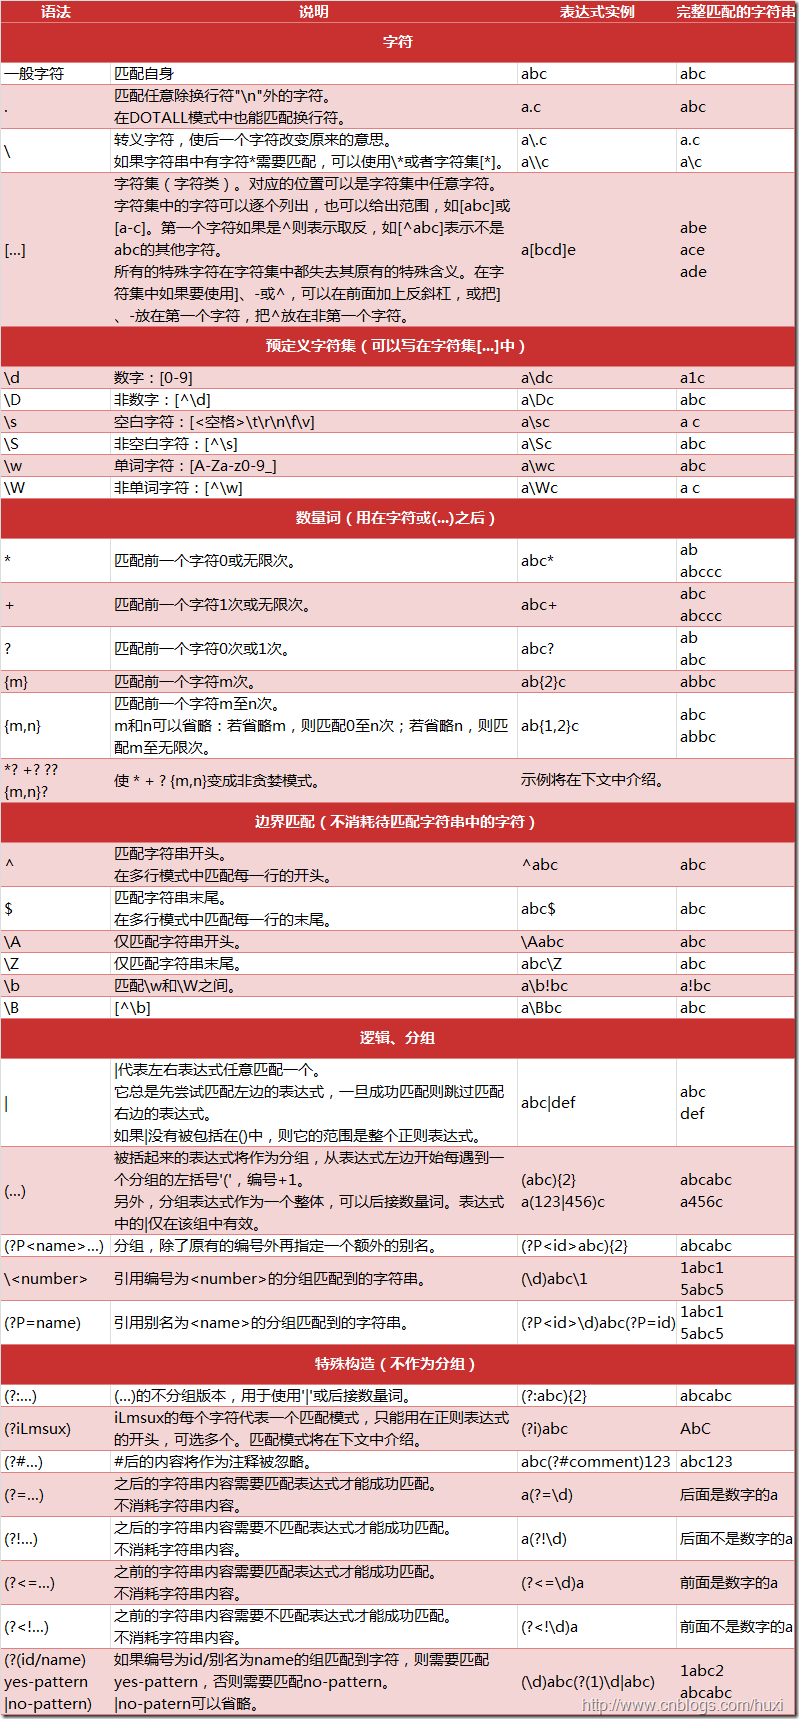
\includegraphics[width=0.95\linewidth,height=0.7\textheight,keepaspectratio]{pyre} \end{center}

图片来源于
\url{https://www.cnblogs.com/huxi/archive/2010/07/04/1771073.html}

\subsection{Python画图}\label{python}

\paragraph{Figure和Subplot}\label{figuresubplot}

\begin{Shaded}
\begin{Highlighting}[]
\ImportTok{import} \NormalTok{matplotlib.pyplot }\ImportTok{as} \NormalTok{plt}
\ImportTok{import} \NormalTok{numpy }\ImportTok{as} \NormalTok{np}
\ImportTok{import} \NormalTok{pandas }\ImportTok{as} \NormalTok{pd}
\ImportTok{from} \NormalTok{numpy.random }\ImportTok{import} \NormalTok{randn}
\end{Highlighting}
\end{Shaded}

\begin{Shaded}
\begin{Highlighting}[]
\NormalTok{x }\OperatorTok{=} \NormalTok{[}\DecValTok{1}\NormalTok{, }\DecValTok{3}\NormalTok{, }\DecValTok{5}\NormalTok{, }\DecValTok{7}\NormalTok{, }\DecValTok{9}\NormalTok{, }\DecValTok{10}\NormalTok{, }\DecValTok{23}\NormalTok{, }\DecValTok{45}\NormalTok{, }\DecValTok{45}\NormalTok{, }\DecValTok{56}\NormalTok{]}
\NormalTok{y }\OperatorTok{=} \NormalTok{[}\DecValTok{2}\NormalTok{, }\DecValTok{4}\NormalTok{, }\DecValTok{6}\NormalTok{, }\DecValTok{8}\NormalTok{, }\DecValTok{11}\NormalTok{, }\DecValTok{12}\NormalTok{, }\DecValTok{23}\NormalTok{, }\DecValTok{45}\NormalTok{, }\DecValTok{56}\NormalTok{, }\DecValTok{78}\NormalTok{]}


\NormalTok{fig }\OperatorTok{=} \NormalTok{plt.figure()}
\NormalTok{ax1 }\OperatorTok{=} \NormalTok{fig.add_subplot(}\DecValTok{2}\NormalTok{, }\DecValTok{2}\NormalTok{, }\DecValTok{1}\NormalTok{)  }\CommentTok{# 创建4个图的Figure对象,最后的1为选中第一个}
\NormalTok{ax2 }\OperatorTok{=} \NormalTok{fig.add_subplot(}\DecValTok{2}\NormalTok{, }\DecValTok{2}\NormalTok{, }\DecValTok{2}\NormalTok{)}
\NormalTok{ax3 }\OperatorTok{=} \NormalTok{fig.add_subplot(}\DecValTok{2}\NormalTok{, }\DecValTok{2}\NormalTok{, }\DecValTok{3}\NormalTok{)}
\NormalTok{ax4 }\OperatorTok{=} \NormalTok{fig.add_subplot(}\DecValTok{2}\NormalTok{, }\DecValTok{2}\NormalTok{, }\DecValTok{4}\NormalTok{)}

\NormalTok{ax1.hist(x, y)}
\NormalTok{ax2.scatter(x, y)}
\NormalTok{ax4.plot(x, y)}

\NormalTok{plt.show()}
\end{Highlighting}
\end{Shaded}

\begin{center}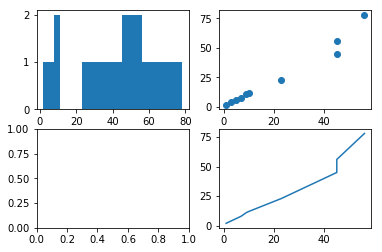
\includegraphics[width=0.95\linewidth,height=0.7\textheight,keepaspectratio]{02_CT_Python_training-chinese_files/02_CT_Python_training-chinese_263_0} \end{center}

\begin{Shaded}
\begin{Highlighting}[]
\NormalTok{fig, axes }\OperatorTok{=} \NormalTok{plt.subplots(}\DecValTok{2}\NormalTok{, }\DecValTok{3}\NormalTok{)}
\NormalTok{axes}
\end{Highlighting}
\end{Shaded}

\begin{verbatim}
array([[<matplotlib.axes._subplots.AxesSubplot object at 0x000000000B5D88D0>,
        <matplotlib.axes._subplots.AxesSubplot object at 0x0000000009A87FD0>,
        <matplotlib.axes._subplots.AxesSubplot object at 0x000000000B3467B8>],
       [<matplotlib.axes._subplots.AxesSubplot object at 0x0000000009CF0390>,
        <matplotlib.axes._subplots.AxesSubplot object at 0x000000000B6CC080>,
        <matplotlib.axes._subplots.AxesSubplot object at 0x000000000B5D9978>]], dtype=object)
\end{verbatim}

\texttt{创建2\ X\ 3图像,可以相当于对二维数组进行索引\ 参数\ \ \ \ \ \ \ \ \ \ \ \ 说明\ nrows\ \ \ \ \ \ \ \ \ \ \ subplot行数\ ncols\ \ \ \ \ \ \ \ \ \ \ subplot列数\ sharex\ \ \ \ \ \ \ \ \ \ 所有图使用相同的x轴\ sharey\ \ \ \ \ \ \ \ \ \ 所有图使用相同的y轴\ subplot\_kw\ \ \ \ \ \ 用于创建各subplot的关键字字典}\textbar{}

\paragraph{调整subplot周围间距}\label{subplot}

\begin{verbatim}
subplots_ajust(left=None,bottom=None,right=None,top=None,wspace=None,hspace=None)
wspace和hspace控制宽度和高度的百分比
\end{verbatim}

\begin{Shaded}
\begin{Highlighting}[]
\NormalTok{fig, axes }\OperatorTok{=} \NormalTok{plt.subplots(}\DecValTok{2}\NormalTok{, }\DecValTok{2}\NormalTok{, sharex}\OperatorTok{=}\VariableTok{True}\NormalTok{, sharey}\OperatorTok{=}\VariableTok{True}\NormalTok{)}
\ControlFlowTok{for} \NormalTok{i }\OperatorTok{in} \BuiltInTok{range}\NormalTok{(}\DecValTok{2}\NormalTok{):}
    \ControlFlowTok{for} \NormalTok{j }\OperatorTok{in} \BuiltInTok{range}\NormalTok{(}\DecValTok{2}\NormalTok{):}
        \NormalTok{axes[i, j].hist(randn(}\DecValTok{500}\NormalTok{), bins}\OperatorTok{=}\DecValTok{50}\NormalTok{, color}\OperatorTok{=}\StringTok{'k'}\NormalTok{, alpha}\OperatorTok{=}\FloatTok{0.5}\NormalTok{)}
\NormalTok{plt.subplots_adjust(wspace}\OperatorTok{=}\DecValTok{0}\NormalTok{, hspace}\OperatorTok{=}\DecValTok{0}\NormalTok{)}
\NormalTok{plt.show()}
\end{Highlighting}
\end{Shaded}

\begin{center}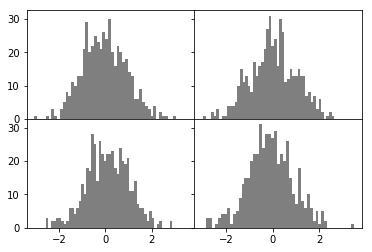
\includegraphics[width=0.95\linewidth,height=0.7\textheight,keepaspectratio]{02_CT_Python_training-chinese_files/02_CT_Python_training-chinese_267_0} \end{center}

\begin{Shaded}
\begin{Highlighting}[]
\NormalTok{fig, axes }\OperatorTok{=} \NormalTok{plt.subplots(}\DecValTok{2}\NormalTok{, }\DecValTok{2}\NormalTok{, sharex}\OperatorTok{=}\VariableTok{True}\NormalTok{, sharey}\OperatorTok{=}\VariableTok{True}\NormalTok{)}
\ControlFlowTok{for} \NormalTok{i }\OperatorTok{in} \BuiltInTok{range}\NormalTok{(}\DecValTok{2}\NormalTok{):}
    \ControlFlowTok{for} \NormalTok{j }\OperatorTok{in} \BuiltInTok{range}\NormalTok{(}\DecValTok{2}\NormalTok{):}
        \NormalTok{axes[i, j].hist(randn(}\DecValTok{500}\NormalTok{), bins}\OperatorTok{=}\DecValTok{50}\NormalTok{, color}\OperatorTok{=}\StringTok{'k'}\NormalTok{, alpha}\OperatorTok{=}\FloatTok{0.5}\NormalTok{)}
\NormalTok{plt.subplots_adjust(wspace}\OperatorTok{=}\DecValTok{1}\NormalTok{, hspace}\OperatorTok{=}\DecValTok{1}\NormalTok{)}
\NormalTok{plt.show()}
\end{Highlighting}
\end{Shaded}

\begin{center}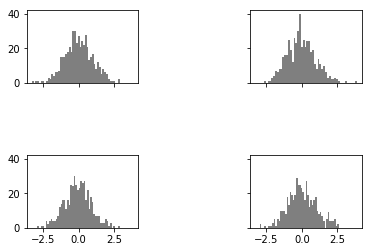
\includegraphics[width=0.95\linewidth,height=0.7\textheight,keepaspectratio]{02_CT_Python_training-chinese_files/02_CT_Python_training-chinese_268_0} \end{center}

\paragraph{颜色 标记和线型}\label{-}

\begin{Shaded}
\begin{Highlighting}[]
\CommentTok{"""}
\CommentTok{绘制绿色虚线}
\CommentTok{ax.plot(x,y,'g--')}
\CommentTok{另一种方式}
\CommentTok{ax.plot(x,y,linestyle='--',color='g')}
\CommentTok{标记点(maker)}
\CommentTok{"""}
\NormalTok{fig, axes }\OperatorTok{=} \NormalTok{plt.subplots(}\DecValTok{1}\NormalTok{, }\DecValTok{2}\NormalTok{)}

\NormalTok{axes[}\DecValTok{0}\NormalTok{].plot(randn(}\DecValTok{10}\NormalTok{), }\StringTok{'g--'}\NormalTok{)  }\CommentTok{# green ---}
\NormalTok{axes[}\DecValTok{1}\NormalTok{].plot(randn(}\DecValTok{10}\NormalTok{), }\StringTok{'ko--'}\NormalTok{)  }\CommentTok{# k:black o:圆点}

\NormalTok{plt.show()}
\end{Highlighting}
\end{Shaded}

\begin{center}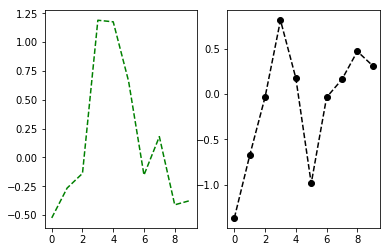
\includegraphics[width=0.95\linewidth,height=0.7\textheight,keepaspectratio]{02_CT_Python_training-chinese_files/02_CT_Python_training-chinese_270_0} \end{center}

\paragraph{刻度、标签和图例}

\begin{Shaded}
\begin{Highlighting}[]
\NormalTok{fig }\OperatorTok{=} \NormalTok{plt.figure()}
\NormalTok{ax }\OperatorTok{=} \NormalTok{fig.add_subplot(}\DecValTok{1}\NormalTok{, }\DecValTok{1}\NormalTok{, }\DecValTok{1}\NormalTok{)}
\NormalTok{ax.plot(randn(}\DecValTok{100}\NormalTok{))}
\NormalTok{plt.show()}
\end{Highlighting}
\end{Shaded}

\begin{center}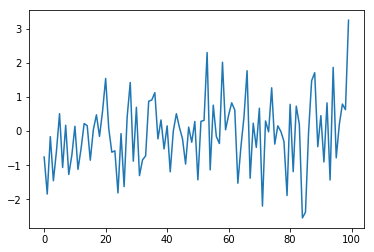
\includegraphics[width=0.95\linewidth,height=0.7\textheight,keepaspectratio]{02_CT_Python_training-chinese_files/02_CT_Python_training-chinese_272_0} \end{center}

\begin{Shaded}
\begin{Highlighting}[]
\CommentTok{"""修改上图的轴"""}

\NormalTok{fig }\OperatorTok{=} \NormalTok{plt.figure()}
\NormalTok{ax }\OperatorTok{=} \NormalTok{fig.add_subplot(}\DecValTok{1}\NormalTok{, }\DecValTok{1}\NormalTok{, }\DecValTok{1}\NormalTok{)}
\NormalTok{ax.plot(randn(}\DecValTok{100}\NormalTok{))}

\NormalTok{ticks }\OperatorTok{=} \NormalTok{ax.set_xticks([}\DecValTok{0}\NormalTok{, }\DecValTok{25}\NormalTok{, }\DecValTok{50}\NormalTok{, }\DecValTok{75}\NormalTok{, }\DecValTok{100}\NormalTok{])  }\CommentTok{# 设置刻度}
\NormalTok{labels }\OperatorTok{=} \NormalTok{ax.set_xticklabels(}
    \NormalTok{[}\StringTok{'first'}\NormalTok{, }\StringTok{'second'}\NormalTok{, }\StringTok{'third'}\NormalTok{, }\StringTok{'forth'}\NormalTok{, }\StringTok{'fifth'}\NormalTok{], rotation}\OperatorTok{=}\DecValTok{30}\NormalTok{, fontsize}\OperatorTok{=}\StringTok{'small'}\NormalTok{)  }\CommentTok{# 设置x轴标签}

\NormalTok{ax.set_title(}\StringTok{'my first matplot plot'}\NormalTok{)  }\CommentTok{# 设置图片标题}

\NormalTok{ax.set_xlabel(}\StringTok{'Stages'}\NormalTok{)  }\CommentTok{# 设置x轴名称}

\NormalTok{plt.show()}
\end{Highlighting}
\end{Shaded}

\begin{center}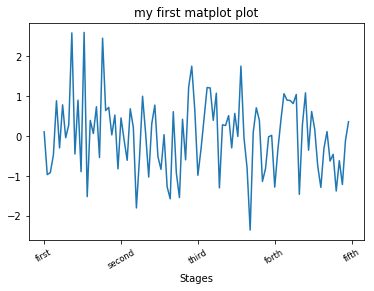
\includegraphics[width=0.95\linewidth,height=0.7\textheight,keepaspectratio]{02_CT_Python_training-chinese_files/02_CT_Python_training-chinese_273_0} \end{center}

\paragraph{添加图例legend}\label{legend}

\begin{verbatim}
https://matplotlib.org/api/legend_api.html?highlight=legend#module-matplotlib.legend
‘best’          0
‘upper right’   1
‘upper left’    2
‘lower left’    3
‘lower right’   4
‘right’         5
‘center left’   6
‘center right’  7
‘lower center’  8
‘upper center’  9
‘center’        10
bbox_to_anchor=(0.5,0.8)
bbox_to_anchor被赋予的二元组中,第一个数值用于控制legend的左右移动,值越大越向右边移动,
第二个数值用于控制legend的上下移动,值越大,越向上移动
\end{verbatim}

\begin{Shaded}
\begin{Highlighting}[]
\NormalTok{fig }\OperatorTok{=} \NormalTok{plt.figure()}
\NormalTok{ax }\OperatorTok{=} \NormalTok{fig.add_subplot(}\DecValTok{1}\NormalTok{, }\DecValTok{1}\NormalTok{, }\DecValTok{1}\NormalTok{)}

\NormalTok{ax.plot(randn(}\DecValTok{10}\NormalTok{), }\StringTok{'k'}\NormalTok{, label}\OperatorTok{=}\StringTok{'one'}\NormalTok{)  }\CommentTok{# 画一条线,k黑色}
\NormalTok{ax.plot(randn(}\DecValTok{10}\NormalTok{), }\StringTok{'g--'}\NormalTok{, label}\OperatorTok{=}\StringTok{'two'}\NormalTok{)  }\CommentTok{# 画第二条线,g绿色 - -类型}
\NormalTok{ax.plot(randn(}\DecValTok{10}\NormalTok{), }\StringTok{'ro--'}\NormalTok{, label}\OperatorTok{=}\StringTok{'three'}\NormalTok{)  }\CommentTok{# 画第三条线红色 ,类型 ...}

\NormalTok{ax.legend(loc}\OperatorTok{=}\DecValTok{0}\NormalTok{, bbox_to_anchor}\OperatorTok{=}\NormalTok{(}\FloatTok{0.5}\NormalTok{, }\FloatTok{0.9}\NormalTok{))}


\NormalTok{plt.show()}
\end{Highlighting}
\end{Shaded}

\begin{center}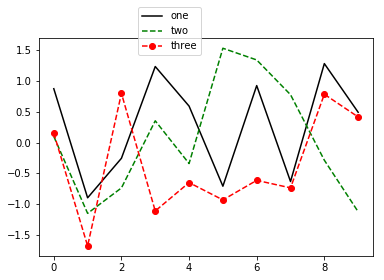
\includegraphics[width=0.95\linewidth,height=0.7\textheight,keepaspectratio]{02_CT_Python_training-chinese_files/02_CT_Python_training-chinese_275_0} \end{center}

\paragraph{注解}

\begin{Shaded}
\begin{Highlighting}[]
\NormalTok{x }\OperatorTok{=} \NormalTok{[}\DecValTok{2}\NormalTok{, }\DecValTok{4}\NormalTok{, }\DecValTok{6}\NormalTok{, }\DecValTok{8}\NormalTok{, }\DecValTok{10}\NormalTok{, }\DecValTok{12}\NormalTok{]}
\NormalTok{y }\OperatorTok{=} \NormalTok{[}\DecValTok{1}\NormalTok{, }\DecValTok{3}\NormalTok{, }\DecValTok{5}\NormalTok{, }\DecValTok{7}\NormalTok{, }\DecValTok{9}\NormalTok{, }\DecValTok{11}\NormalTok{]}
\NormalTok{fig }\OperatorTok{=} \NormalTok{plt.figure()}
\NormalTok{ax }\OperatorTok{=} \NormalTok{fig.add_subplot(}\DecValTok{1}\NormalTok{, }\DecValTok{1}\NormalTok{, }\DecValTok{1}\NormalTok{)}
\CommentTok{##ax = fig}
\NormalTok{ax.plot(x, y, }\StringTok{'r--'}\NormalTok{)}

\NormalTok{ax.text(}\DecValTok{2}\NormalTok{, }\DecValTok{4}\NormalTok{, }\StringTok{'hello python'}\NormalTok{)}
\NormalTok{plt.show()}
\end{Highlighting}
\end{Shaded}

\begin{center}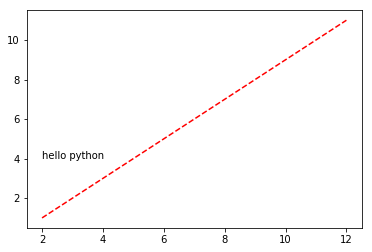
\includegraphics[width=0.95\linewidth,height=0.7\textheight,keepaspectratio]{02_CT_Python_training-chinese_files/02_CT_Python_training-chinese_277_0} \end{center}

\paragraph{图片保存}

\begin{Shaded}
\begin{Highlighting}[]
\NormalTok{x }\OperatorTok{=} \NormalTok{[}\DecValTok{2}\NormalTok{, }\DecValTok{4}\NormalTok{, }\DecValTok{6}\NormalTok{, }\DecValTok{8}\NormalTok{, }\DecValTok{10}\NormalTok{, }\DecValTok{12}\NormalTok{]}
\NormalTok{y }\OperatorTok{=} \NormalTok{[}\DecValTok{1}\NormalTok{, }\DecValTok{3}\NormalTok{, }\DecValTok{5}\NormalTok{, }\DecValTok{7}\NormalTok{, }\DecValTok{9}\NormalTok{, }\DecValTok{11}\NormalTok{]}
\NormalTok{fig }\OperatorTok{=} \NormalTok{plt.figure()}
\NormalTok{ax }\OperatorTok{=} \NormalTok{fig.add_subplot(}\DecValTok{1}\NormalTok{, }\DecValTok{1}\NormalTok{, }\DecValTok{1}\NormalTok{)}
\NormalTok{ax.plot(x, y, }\StringTok{'r--'}\NormalTok{)}

\NormalTok{ax.text(}\DecValTok{2}\NormalTok{, }\DecValTok{4}\NormalTok{, }\StringTok{'hello python'}\NormalTok{)}

\CommentTok{## bbox_inches减除当前图片周围空白部分}
\NormalTok{plt.savefig(}\StringTok{'figpath.jpg'}\NormalTok{, dpi}\OperatorTok{=}\DecValTok{300}\NormalTok{, bbox_inches}\OperatorTok{=}\StringTok{'tight'}\NormalTok{)}
\end{Highlighting}
\end{Shaded}

\paragraph{matplotlib配置
绘图之前可以调整各种参数字体,全局所有图片的大小等。}\label{matplotlib-}

实例

\subparagraph{绘制散点图}

\begin{Shaded}
\begin{Highlighting}[]
\NormalTok{x }\OperatorTok{=} \NormalTok{[}\DecValTok{1}\NormalTok{, }\DecValTok{2}\NormalTok{, }\DecValTok{3}\NormalTok{, }\DecValTok{4}\NormalTok{, }\DecValTok{5}\NormalTok{, }\DecValTok{6}\NormalTok{]}
\NormalTok{y }\OperatorTok{=} \NormalTok{[}\DecValTok{1}\NormalTok{, }\DecValTok{4}\NormalTok{, }\DecValTok{9}\NormalTok{, }\DecValTok{16}\NormalTok{, }\DecValTok{25}\NormalTok{, }\DecValTok{36}\NormalTok{]}
\NormalTok{plt.scatter(x,  }\CommentTok{# x轴数据为汽车速度}
            \NormalTok{y,  }\CommentTok{# y轴数据为汽车的刹车距离}
            \NormalTok{s}\OperatorTok{=}\DecValTok{20}\NormalTok{,  }\CommentTok{# 设置点的大小}
            \NormalTok{c}\OperatorTok{=}\StringTok{'green'}\NormalTok{,  }\CommentTok{# 设置点的颜色}
            \NormalTok{marker}\OperatorTok{=}\StringTok{'s'}\NormalTok{,  }\CommentTok{# 设置点的形状}
            \NormalTok{alpha}\OperatorTok{=}\FloatTok{0.9}\NormalTok{,  }\CommentTok{# 设置点的透明度}
            \NormalTok{linewidths}\OperatorTok{=}\FloatTok{0.8}\NormalTok{,  }\CommentTok{# 设置散点边界的粗细}
            \NormalTok{edgecolors}\OperatorTok{=}\StringTok{'red'}  \CommentTok{# 设置散点边界的颜色}
            \NormalTok{)}

\NormalTok{plt.title(}\StringTok{'simple scatter plot'}\NormalTok{)}
\NormalTok{plt.xlabel(}\StringTok{'X'}\NormalTok{)  }\CommentTok{# x轴名称}
\NormalTok{plt.ylabel(}\StringTok{'Y'}\NormalTok{)}

\NormalTok{plt.show()  }\CommentTok{# 展示绘图}
\end{Highlighting}
\end{Shaded}

\begin{center}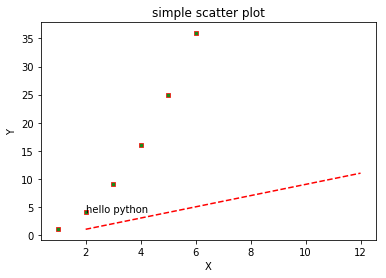
\includegraphics[width=0.95\linewidth,height=0.7\textheight,keepaspectratio]{02_CT_Python_training-chinese_files/02_CT_Python_training-chinese_283_0} \end{center}

\subparagraph{折线图}

\begin{Shaded}
\begin{Highlighting}[]
\NormalTok{x }\OperatorTok{=} \NormalTok{[}\DecValTok{1}\NormalTok{, }\DecValTok{2}\NormalTok{, }\DecValTok{3}\NormalTok{, }\DecValTok{4}\NormalTok{, }\DecValTok{5}\NormalTok{, }\DecValTok{6}\NormalTok{]}
\NormalTok{y }\OperatorTok{=} \NormalTok{[}\DecValTok{1}\NormalTok{, }\DecValTok{4}\NormalTok{, }\DecValTok{9}\NormalTok{, }\DecValTok{16}\NormalTok{, }\DecValTok{25}\NormalTok{, }\DecValTok{36}\NormalTok{]}

\NormalTok{plt.plot(x,  }\CommentTok{# x轴数据}
         \NormalTok{y,  }\CommentTok{# y轴数据}
         \NormalTok{linestyle}\OperatorTok{=}\StringTok{'-'}\NormalTok{,  }\CommentTok{# 折线类型}
         \NormalTok{linewidth}\OperatorTok{=}\DecValTok{2}\NormalTok{,  }\CommentTok{# 折线宽度}
         \NormalTok{color}\OperatorTok{=}\StringTok{'blue'}\NormalTok{,  }\CommentTok{# 折线颜色}
         \NormalTok{marker}\OperatorTok{=}\StringTok{'o'}\NormalTok{,  }\CommentTok{# 点的形状}
         \NormalTok{markersize}\OperatorTok{=}\DecValTok{8}\NormalTok{,  }\CommentTok{# 点的大小}
         \NormalTok{markeredgecolor}\OperatorTok{=}\StringTok{'black'}\NormalTok{,  }\CommentTok{# 点的边框色}
         \NormalTok{markerfacecolor}\OperatorTok{=}\StringTok{'red'}\NormalTok{)  }\CommentTok{# 点的填充色}

\CommentTok{## 添加标题和坐标轴标签}
\NormalTok{plt.title(}\StringTok{'line plot'}\NormalTok{)}
\NormalTok{plt.xlabel(}\StringTok{'X'}\NormalTok{)}
\NormalTok{plt.ylabel(}\StringTok{'Y'}\NormalTok{)}

\NormalTok{plt.show()}
\end{Highlighting}
\end{Shaded}

\begin{center}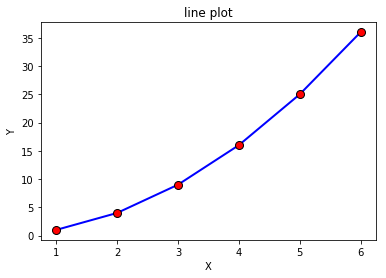
\includegraphics[width=0.95\linewidth,height=0.7\textheight,keepaspectratio]{02_CT_Python_training-chinese_files/02_CT_Python_training-chinese_285_0} \end{center}

\subparagraph{直方图}

\begin{Shaded}
\begin{Highlighting}[]
\ImportTok{import} \NormalTok{numpy }\ImportTok{as} \NormalTok{np}
\ImportTok{import} \NormalTok{pandas }\ImportTok{as} \NormalTok{pd}
\ImportTok{import} \NormalTok{matplotlib.pyplot }\ImportTok{as} \NormalTok{plt}

\NormalTok{plt.hist(np.random.randn(}\DecValTok{50}\NormalTok{),  }\CommentTok{# 绘图数据}
         \NormalTok{bins}\OperatorTok{=}\DecValTok{50}\NormalTok{,  }\CommentTok{# 指定直方图的条形数为20个}
         \NormalTok{color}\OperatorTok{=}\StringTok{'red'}\NormalTok{,  }\CommentTok{# 指定填充色}
         \NormalTok{edgecolor}\OperatorTok{=}\StringTok{'k'}\NormalTok{,  }\CommentTok{# 指定直方图的边界色}
         \NormalTok{label}\OperatorTok{=}\StringTok{'histogram'}\NormalTok{)  }\CommentTok{# 为直方图呈现标签}
\NormalTok{plt.show()}
\end{Highlighting}
\end{Shaded}

\begin{center}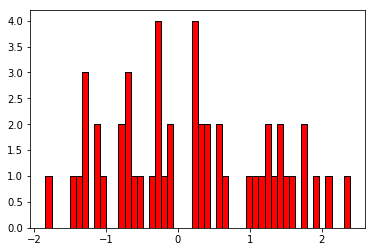
\includegraphics[width=0.95\linewidth,height=0.7\textheight,keepaspectratio]{02_CT_Python_training-chinese_files/02_CT_Python_training-chinese_287_0} \end{center}

\paragraph{直条图}

\begin{Shaded}
\begin{Highlighting}[]
\NormalTok{x }\OperatorTok{=} \NormalTok{[}\DecValTok{1}\NormalTok{, }\DecValTok{2}\NormalTok{, }\DecValTok{3}\NormalTok{, }\DecValTok{4}\NormalTok{, }\DecValTok{5}\NormalTok{, }\DecValTok{6}\NormalTok{]}
\NormalTok{y }\OperatorTok{=} \NormalTok{[}\DecValTok{1}\NormalTok{, }\DecValTok{4}\NormalTok{, }\DecValTok{9}\NormalTok{, }\DecValTok{16}\NormalTok{, }\DecValTok{25}\NormalTok{, }\DecValTok{36}\NormalTok{]}

\NormalTok{plt.bar(x, y,}
        \NormalTok{color}\OperatorTok{=}\StringTok{'steelblue'}\NormalTok{,}
        \NormalTok{alpha}\OperatorTok{=}\FloatTok{0.8}\NormalTok{)}

\NormalTok{plt.title(}\StringTok{'bar plot'}\NormalTok{)}

\NormalTok{plt.ylim([}\DecValTok{0}\NormalTok{, }\DecValTok{40}\NormalTok{])}
\NormalTok{plt.show()}
\end{Highlighting}
\end{Shaded}

\begin{center}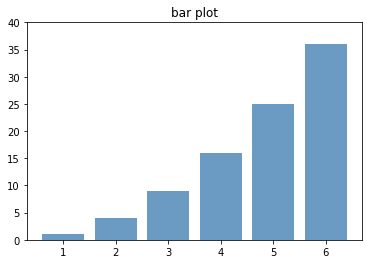
\includegraphics[width=0.95\linewidth,height=0.7\textheight,keepaspectratio]{02_CT_Python_training-chinese_files/02_CT_Python_training-chinese_289_0} \end{center}

\begin{Shaded}
\begin{Highlighting}[]
\NormalTok{x }\OperatorTok{=} \NormalTok{[}\DecValTok{1}\NormalTok{, }\DecValTok{2}\NormalTok{, }\DecValTok{3}\NormalTok{, }\DecValTok{4}\NormalTok{, }\DecValTok{5}\NormalTok{, }\DecValTok{6}\NormalTok{]}
\NormalTok{y }\OperatorTok{=} \NormalTok{[}\DecValTok{1}\NormalTok{, }\DecValTok{4}\NormalTok{, }\DecValTok{9}\NormalTok{, }\DecValTok{16}\NormalTok{, }\DecValTok{25}\NormalTok{, }\DecValTok{36}\NormalTok{]}

\NormalTok{plt.barh(x, y,}
         \NormalTok{color}\OperatorTok{=}\StringTok{'steelblue'}\NormalTok{,}
         \NormalTok{alpha}\OperatorTok{=}\FloatTok{0.8}\NormalTok{)}

\NormalTok{plt.title(}\StringTok{'bar plot'}\NormalTok{)}

\NormalTok{plt.show()}
\end{Highlighting}
\end{Shaded}

\begin{center}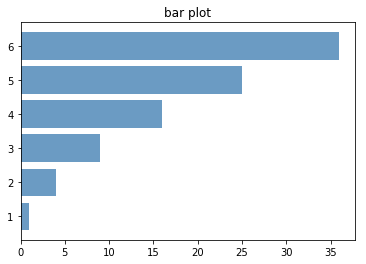
\includegraphics[width=0.95\linewidth,height=0.7\textheight,keepaspectratio]{02_CT_Python_training-chinese_files/02_CT_Python_training-chinese_290_0} \end{center}

\paragraph{箱线图}

\begin{Shaded}
\begin{Highlighting}[]
\NormalTok{x }\OperatorTok{=} \NormalTok{[}\DecValTok{1}\NormalTok{, }\DecValTok{2}\NormalTok{, }\DecValTok{3}\NormalTok{, }\DecValTok{4}\NormalTok{, }\DecValTok{5}\NormalTok{, }\DecValTok{6}\NormalTok{]}
\NormalTok{plt.boxplot(x,}
            \NormalTok{patch_artist}\OperatorTok{=}\VariableTok{True}\NormalTok{,  }\CommentTok{# 箱体添加颜色}
            \NormalTok{labels}\OperatorTok{=}\NormalTok{[}\StringTok{'boxplot'}\NormalTok{],  }\CommentTok{# 添加具体的标签名称}
            \NormalTok{showmeans}\OperatorTok{=}\VariableTok{True}\NormalTok{, )}

\CommentTok{## 显示图形}
\NormalTok{plt.show()}
\end{Highlighting}
\end{Shaded}

\begin{center}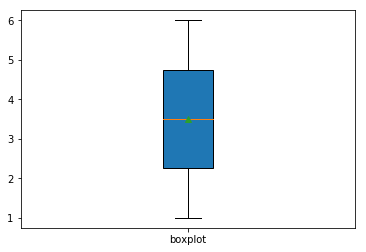
\includegraphics[width=0.95\linewidth,height=0.7\textheight,keepaspectratio]{02_CT_Python_training-chinese_files/02_CT_Python_training-chinese_292_0} \end{center}

\begin{Shaded}
\begin{Highlighting}[]
\NormalTok{np.random.seed(}\DecValTok{2}\NormalTok{)  }\CommentTok{# 设置随机种子}
\NormalTok{df }\OperatorTok{=} \NormalTok{pd.DataFrame(np.random.rand(}\DecValTok{5}\NormalTok{, }\DecValTok{4}\NormalTok{),}
                  \NormalTok{columns}\OperatorTok{=}\NormalTok{([}\StringTok{'A'}\NormalTok{, }\StringTok{'B'}\NormalTok{, }\StringTok{'C'}\NormalTok{, }\StringTok{'D'}\NormalTok{]))}
\NormalTok{df}
\end{Highlighting}
\end{Shaded}

\begin{verbatim}
<tr style="text-align: right;">
  <th></th>
  <th>A</th>
  <th>B</th>
  <th>C</th>
  <th>D</th>
</tr>
\end{verbatim}

\begin{verbatim}
<tr>
  <th>0</th>
  <td>0.435995</td>
  <td>0.025926</td>
  <td>0.549662</td>
  <td>0.435322</td>
</tr>
<tr>
  <th>1</th>
  <td>0.420368</td>
  <td>0.330335</td>
  <td>0.204649</td>
  <td>0.619271</td>
</tr>
<tr>
  <th>2</th>
  <td>0.299655</td>
  <td>0.266827</td>
  <td>0.621134</td>
  <td>0.529142</td>
</tr>
<tr>
  <th>3</th>
  <td>0.134580</td>
  <td>0.513578</td>
  <td>0.184440</td>
  <td>0.785335</td>
</tr>
<tr>
  <th>4</th>
  <td>0.853975</td>
  <td>0.494237</td>
  <td>0.846561</td>
  <td>0.079645</td>
</tr>
\end{verbatim}

\begin{Shaded}
\begin{Highlighting}[]
\NormalTok{data }\OperatorTok{=} \NormalTok{[]}
\ControlFlowTok{for} \NormalTok{i }\OperatorTok{in} \BuiltInTok{range}\NormalTok{(}\DecValTok{4}\NormalTok{):}
    \NormalTok{data.append(df.iloc[:, i])}
\NormalTok{data}
\end{Highlighting}
\end{Shaded}

\begin{verbatim}
[0    0.435995
 1    0.420368
 2    0.299655
 3    0.134580
 4    0.853975
 Name: A, dtype: float64, 0    0.025926
 1    0.330335
 2    0.266827
 3    0.513578
 4    0.494237
 Name: B, dtype: float64, 0    0.549662
 1    0.204649
 2    0.621134
 3    0.184440
 4    0.846561
 Name: C, dtype: float64, 0    0.435322
 1    0.619271
 2    0.529142
 3    0.785335
 4    0.079645
 Name: D, dtype: float64]
\end{verbatim}

\begin{Shaded}
\begin{Highlighting}[]
\NormalTok{plt.boxplot(data)}
\NormalTok{plt.show()}
\end{Highlighting}
\end{Shaded}

\begin{center}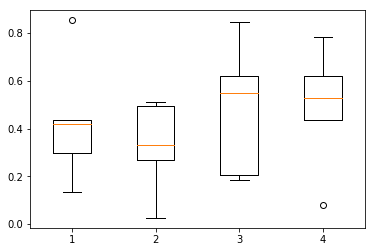
\includegraphics[width=0.95\linewidth,height=0.7\textheight,keepaspectratio]{02_CT_Python_training-chinese_files/02_CT_Python_training-chinese_295_0} \end{center}

\begin{verbatim}
plt.boxplot(x, notch=None, sym=None, vert=None, 
             whis=None, positions=None, widths=None, 
             patch_artist=None, meanline=None, showmeans=None, 
             showcaps=None, showbox=None, showfliers=None, 
             boxprops=None, labels=None, flierprops=None, 
             medianprops=None, meanprops=None, 
             capprops=None, whiskerprops=None)

x:指定要绘制箱线图的数据;
notch:是否是凹口的形式展现箱线图,默认非凹口;
sym:指定异常点的形状,默认为+号显示;
vert:是否需要将箱线图垂直摆放,默认垂直摆放;
whis:指定上下须与上下四分位的距离,默认为1.5倍的四分位差;
positions:指定箱线图的位置,默认为[0,1,2…];
widths:指定箱线图的宽度,默认为0.5;
patch_artist:是否填充箱体的颜色;
meanline:是否用线的形式表示均值,默认用点来表示;
showmeans:是否显示均值,默认不显示;
showcaps:是否显示箱线图顶端和末端的两条线,默认显示;
showbox:是否显示箱线图的箱体,默认显示;
showfliers:是否显示异常值,默认显示;
boxprops:设置箱体的属性,如边框色,填充色等;
labels:为箱线图添加标签,类似于图例的作用;
filerprops:设置异常值的属性,如异常点的形状、大小、填充色等;
medianprops:设置中位数的属性,如线的类型、粗细等;
meanprops:设置均值的属性,如点的大小、颜色等;
capprops:设置箱线图顶端和末端线条的属性,如颜色、粗细等;
whiskerprops:设置须的属性,如颜色、粗细、线的类型等;
\end{verbatim}

\subparagraph{饼图}

\begin{Shaded}
\begin{Highlighting}[]
\NormalTok{data }\OperatorTok{=} \NormalTok{[}\FloatTok{0.2}\NormalTok{, }\FloatTok{0.3}\NormalTok{, }\FloatTok{0.4}\NormalTok{, }\FloatTok{0.1}\NormalTok{]}
\NormalTok{plt.pie(data)}
\NormalTok{plt.show()}
\end{Highlighting}
\end{Shaded}

\begin{center}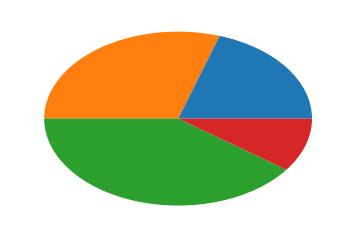
\includegraphics[width=0.95\linewidth,height=0.7\textheight,keepaspectratio]{02_CT_Python_training-chinese_files/02_CT_Python_training-chinese_298_0} \end{center}

\begin{verbatim}
plt.pie(x, explode=None, labels=None, colors=None, 
        autopct=None, pctdistance=0.6, shadow=False, 
        labeldistance=1.1, startangle=None, 
        radius=None, counterclock=True, wedgeprops=None, 
        textprops=None, center=(0, 0), frame=False)
        
x:指定绘图的数据;
explode:指定饼图某些部分的突出显示,即呈现爆炸式;
labels:为饼图添加标签说明,类似于图例说明;
colors:指定饼图的填充色;
autopct:自动添加百分比显示,可以采用格式化的方法显示;
pctdistance:设置百分比标签与圆心的距离;
shadow:是否添加饼图的阴影效果;
labeldistance:设置各扇形标签(图例)与圆心的距离;
startangle:设置饼图的初始摆放角度;
radius:设置饼图的半径大小;
counterclock:是否让饼图按逆时针顺序呈现;
wedgeprops:设置饼图内外边界的属性,如边界线的粗细、颜色等;
textprops:设置饼图中文本的属性,如字体大小、颜色等;
center:指定饼图的中心点位置,默认为原点
frame:是否要显示饼图背后的图框,如果设置为True的话,需要同时控制图框x轴、y轴的范围和饼图的中心位置;
\end{verbatim}

\begin{Shaded}
\begin{Highlighting}[]

\end{Highlighting}
\end{Shaded}

\begin{Shaded}
\begin{Highlighting}[]
\OperatorTok{%}\NormalTok{matplotlib inline}
\ImportTok{from} \NormalTok{mpl_toolkits.mplot3d }\ImportTok{import} \NormalTok{axes3d}
\ImportTok{import} \NormalTok{matplotlib.pyplot }\ImportTok{as} \NormalTok{plt}
\ImportTok{from} \NormalTok{matplotlib }\ImportTok{import} \NormalTok{cm}

\NormalTok{fig }\OperatorTok{=} \NormalTok{plt.figure()}
\NormalTok{ax }\OperatorTok{=} \NormalTok{fig.add_subplot(}\DecValTok{111}\NormalTok{, projection}\OperatorTok{=}\StringTok{'3d'}\NormalTok{)}
\NormalTok{X, Y, Z }\OperatorTok{=} \NormalTok{axes3d.get_test_data(}\FloatTok{0.05}\NormalTok{)}
\NormalTok{cset }\OperatorTok{=} \NormalTok{ax.contour(X, Y, Z, cmap}\OperatorTok{=}\NormalTok{cm.coolwarm)}
\NormalTok{ax.clabel(cset, fontsize}\OperatorTok{=}\DecValTok{9}\NormalTok{, inline}\OperatorTok{=}\DecValTok{1}\NormalTok{)}

\NormalTok{plt.show()}
\end{Highlighting}
\end{Shaded}

\begin{center}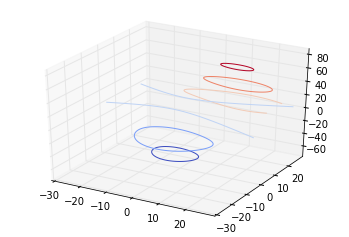
\includegraphics[width=0.95\linewidth,height=0.7\textheight,keepaspectratio]{02_CT_Python_training-chinese_files/02_CT_Python_training-chinese_301_0} \end{center}

\begin{Shaded}
\begin{Highlighting}[]
\ImportTok{import} \NormalTok{matplotlib }\ImportTok{as} \NormalTok{mpl}
\ImportTok{from} \NormalTok{mpl_toolkits.mplot3d }\ImportTok{import} \NormalTok{Axes3D}
\ImportTok{import} \NormalTok{numpy }\ImportTok{as} \NormalTok{np}
\ImportTok{import} \NormalTok{matplotlib.pyplot }\ImportTok{as} \NormalTok{plt}

\NormalTok{mpl.rcParams[}\StringTok{'legend.fontsize'}\NormalTok{] }\OperatorTok{=} \DecValTok{10}

\NormalTok{fig }\OperatorTok{=} \NormalTok{plt.figure()}
\NormalTok{ax }\OperatorTok{=} \NormalTok{fig.gca(projection}\OperatorTok{=}\StringTok{'3d'}\NormalTok{)}
\CommentTok{##theta = np.linspace(-4 * np.pi, 4 * np.pi, 100)}
\CommentTok{##z = np.linspace(-2, 2, 100)}
\CommentTok{##r = z**2 + 1}
\CommentTok{##x = r * np.sin(theta)}
\CommentTok{##y = r * np.cos(theta)}
\NormalTok{x }\OperatorTok{=} \NormalTok{[}\DecValTok{1}\NormalTok{, }\DecValTok{2}\NormalTok{, }\DecValTok{3}\NormalTok{]}
\NormalTok{y }\OperatorTok{=} \NormalTok{[}\FloatTok{1.5}\NormalTok{, }\DecValTok{1}\NormalTok{, }\DecValTok{2}\NormalTok{]}
\NormalTok{z }\OperatorTok{=} \NormalTok{[}\DecValTok{2}\NormalTok{, }\DecValTok{1}\NormalTok{, }\DecValTok{3}\NormalTok{]}
\NormalTok{ax.plot(x, y, z, label}\OperatorTok{=}\StringTok{'parametric curve'}\NormalTok{)}
\NormalTok{ax.legend()}

\NormalTok{plt.show()}
\end{Highlighting}
\end{Shaded}

\begin{center}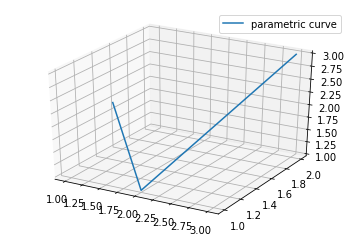
\includegraphics[width=0.95\linewidth,height=0.7\textheight,keepaspectratio]{02_CT_Python_training-chinese_files/02_CT_Python_training-chinese_302_0} \end{center}

\begin{Shaded}
\begin{Highlighting}[]
\ImportTok{from} \NormalTok{matplotlib }\ImportTok{import} \NormalTok{pyplot }\ImportTok{as} \NormalTok{plt}
\ImportTok{from} \NormalTok{matplotlib.patches }\ImportTok{import} \NormalTok{Rectangle}
\NormalTok{someX, someY }\OperatorTok{=} \FloatTok{0.5}\NormalTok{, }\FloatTok{0.5}
\NormalTok{fig, ax }\OperatorTok{=} \NormalTok{plt.subplots()}
\NormalTok{currentAxis }\OperatorTok{=} \NormalTok{plt.gca()}
\NormalTok{currentAxis.add_patch(Rectangle((someX }\OperatorTok{-} \FloatTok{0.1}\NormalTok{, someY }\OperatorTok{-} \FloatTok{0.1}\NormalTok{), }\FloatTok{0.2}\NormalTok{, }\FloatTok{0.2}\NormalTok{,}
                                \NormalTok{alpha}\OperatorTok{=}\DecValTok{1}\NormalTok{, facecolor}\OperatorTok{=}\StringTok{'none'}\NormalTok{))}
\NormalTok{plt.show()}
\end{Highlighting}
\end{Shaded}

\begin{center}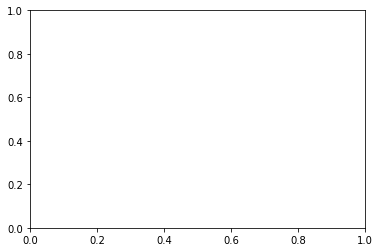
\includegraphics[width=0.95\linewidth,height=0.7\textheight,keepaspectratio]{02_CT_Python_training-chinese_files/02_CT_Python_training-chinese_303_0} \end{center}

\begin{Shaded}
\begin{Highlighting}[]
\ImportTok{from} \NormalTok{mpl_toolkits.mplot3d }\ImportTok{import} \NormalTok{Axes3D}
\ImportTok{from} \NormalTok{mpl_toolkits.mplot3d.art3d }\ImportTok{import} \NormalTok{Poly3DCollection}
\ImportTok{import} \NormalTok{matplotlib.pyplot }\ImportTok{as} \NormalTok{plt}
\NormalTok{fig }\OperatorTok{=} \NormalTok{plt.figure()}
\NormalTok{ax }\OperatorTok{=} \NormalTok{Axes3D(fig)}

\NormalTok{x }\OperatorTok{=} \NormalTok{[}\DecValTok{1}\NormalTok{,}\DecValTok{2}\NormalTok{,}\DecValTok{2}\NormalTok{]}
\NormalTok{y }\OperatorTok{=} \NormalTok{[}\DecValTok{1}\NormalTok{,}\DecValTok{0}\NormalTok{,}\DecValTok{2}\NormalTok{]}
\NormalTok{z }\OperatorTok{=} \NormalTok{[}\DecValTok{1}\NormalTok{,}\DecValTok{2}\NormalTok{,}\DecValTok{0}\NormalTok{]}
\NormalTok{verts }\OperatorTok{=} \NormalTok{[}\BuiltInTok{zip}\NormalTok{(x, y,z)]}
\NormalTok{ax.add_collection3d(Poly3DCollection(verts,edgecolors}\OperatorTok{=}\StringTok{'red'}\NormalTok{, facecolors}\OperatorTok{=}\StringTok{'red'}\NormalTok{))}
\NormalTok{x }\OperatorTok{=} \NormalTok{[}\DecValTok{0}\NormalTok{,}\DecValTok{1}\NormalTok{,}\DecValTok{1}\NormalTok{]}
\NormalTok{y }\OperatorTok{=} \NormalTok{[}\DecValTok{0}\NormalTok{,}\DecValTok{0}\NormalTok{,}\DecValTok{1}\NormalTok{]}
\NormalTok{z }\OperatorTok{=} \NormalTok{[}\DecValTok{0}\NormalTok{,}\DecValTok{1}\NormalTok{,}\DecValTok{0}\NormalTok{]}
\NormalTok{verts }\OperatorTok{=} \NormalTok{[}\BuiltInTok{zip}\NormalTok{(x, y,z)]}
\NormalTok{verts }\OperatorTok{=} \NormalTok{[[(}\DecValTok{1}\NormalTok{,}\DecValTok{1}\NormalTok{,}\DecValTok{1}\NormalTok{), (}\DecValTok{2}\NormalTok{,}\DecValTok{0}\NormalTok{,}\DecValTok{2}\NormalTok{),(}\DecValTok{2}\NormalTok{,}\DecValTok{2}\NormalTok{,}\DecValTok{0}\NormalTok{)],[(}\DecValTok{0}\NormalTok{,}\DecValTok{0}\NormalTok{,}\DecValTok{0}\NormalTok{),(}\DecValTok{1}\NormalTok{,}\DecValTok{0}\NormalTok{,}\DecValTok{1}\NormalTok{),(}\DecValTok{1}\NormalTok{,}\DecValTok{1}\NormalTok{,}\DecValTok{0}\NormalTok{)]]}
\NormalTok{ax.add_collection3d(Poly3DCollection(verts))}
\NormalTok{plt.show()}
\end{Highlighting}
\end{Shaded}

\begin{center}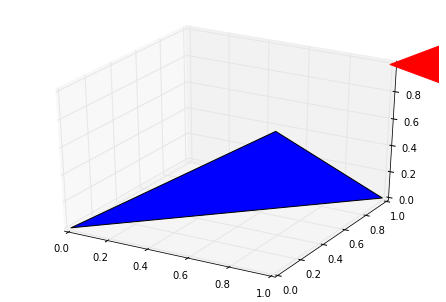
\includegraphics[width=0.95\linewidth,height=0.7\textheight,keepaspectratio]{02_CT_Python_training-chinese_files/02_CT_Python_training-chinese_304_0} \end{center}

\begin{Shaded}
\begin{Highlighting}[]
\ImportTok{from} \NormalTok{mpl_toolkits.mplot3d }\ImportTok{import} \NormalTok{Axes3D}
\ImportTok{from} \NormalTok{mpl_toolkits.mplot3d.art3d }\ImportTok{import} \NormalTok{Poly3DCollection}
\ImportTok{import} \NormalTok{matplotlib.pyplot }\ImportTok{as} \NormalTok{plt}
\NormalTok{fig }\OperatorTok{=} \NormalTok{plt.figure()}
\NormalTok{ax }\OperatorTok{=} \NormalTok{Axes3D(fig)}

\NormalTok{verts }\OperatorTok{=} \NormalTok{[[(}\FloatTok{0.5}\NormalTok{,}\FloatTok{0.5}\NormalTok{,}\FloatTok{0.5}\NormalTok{), (}\FloatTok{1.2}\NormalTok{,}\DecValTok{0}\NormalTok{,}\FloatTok{1.2}\NormalTok{),(}\FloatTok{1.2}\NormalTok{,}\FloatTok{1.2}\NormalTok{,}\DecValTok{0}\NormalTok{)],[(}\DecValTok{0}\NormalTok{,}\DecValTok{0}\NormalTok{,}\DecValTok{0}\NormalTok{),(}\DecValTok{1}\NormalTok{,}\DecValTok{0}\NormalTok{,}\DecValTok{1}\NormalTok{),(}\DecValTok{1}\NormalTok{,}\DecValTok{1}\NormalTok{,}\DecValTok{0}\NormalTok{)]]}
\NormalTok{ax.add_collection3d(Poly3DCollection(verts, edgecolors}\OperatorTok{=}\NormalTok{[}\StringTok{'blue'}\NormalTok{,}\StringTok{'red'}\NormalTok{], facecolors}\OperatorTok{=}\NormalTok{[}\StringTok{'blue'}\NormalTok{,}\StringTok{'red'}\NormalTok{]))}
\NormalTok{plt.show()}
\end{Highlighting}
\end{Shaded}

\begin{center}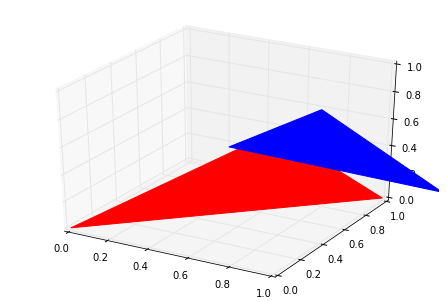
\includegraphics[width=0.95\linewidth,height=0.7\textheight,keepaspectratio]{02_CT_Python_training-chinese_files/02_CT_Python_training-chinese_305_0} \end{center}

\begin{Shaded}
\begin{Highlighting}[]
\ImportTok{from} \NormalTok{matplotlib }\ImportTok{import} \NormalTok{pyplot }\ImportTok{as} \NormalTok{plt}
\ImportTok{from} \NormalTok{mpl_toolkits.mplot3d.art3d }\ImportTok{import} \NormalTok{Poly3DCollection}

\NormalTok{fig }\OperatorTok{=} \NormalTok{plt.figure()}
\NormalTok{ax }\OperatorTok{=} \NormalTok{fig.add_subplot(}\DecValTok{111}\NormalTok{, projection}\OperatorTok{=}\StringTok{'3d'}\NormalTok{)}

\NormalTok{x }\OperatorTok{=} \NormalTok{[}\FloatTok{0.5}\NormalTok{, }\FloatTok{1.2}\NormalTok{, }\FloatTok{1.2}\NormalTok{, }\DecValTok{0}\NormalTok{, }\DecValTok{1}\NormalTok{, }\DecValTok{1}\NormalTok{]}
\NormalTok{y }\OperatorTok{=} \NormalTok{[}\FloatTok{0.5}\NormalTok{, }\DecValTok{0}\NormalTok{,   }\FloatTok{1.2}\NormalTok{, }\DecValTok{0}\NormalTok{, }\DecValTok{0}\NormalTok{, }\DecValTok{1}\NormalTok{]}
\NormalTok{z }\OperatorTok{=} \NormalTok{[}\FloatTok{0.5}\NormalTok{, }\FloatTok{1.2}\NormalTok{, }\DecValTok{0}\NormalTok{,   }\DecValTok{0}\NormalTok{, }\DecValTok{1}\NormalTok{, }\DecValTok{0}\NormalTok{]}

\NormalTok{poly3d }\OperatorTok{=} \NormalTok{[[(}\FloatTok{0.5}\NormalTok{,}\FloatTok{0.5}\NormalTok{,}\FloatTok{0.5}\NormalTok{), (}\FloatTok{1.2}\NormalTok{,}\DecValTok{0}\NormalTok{,}\FloatTok{1.2}\NormalTok{),(}\FloatTok{1.2}\NormalTok{,}\FloatTok{1.2}\NormalTok{,}\DecValTok{0}\NormalTok{)],[(}\DecValTok{0}\NormalTok{,}\DecValTok{0}\NormalTok{,}\DecValTok{0}\NormalTok{),(}\DecValTok{1}\NormalTok{,}\DecValTok{0}\NormalTok{,}\DecValTok{1}\NormalTok{),(}\DecValTok{1}\NormalTok{,}\DecValTok{1}\NormalTok{,}\DecValTok{0}\NormalTok{)]]}
\NormalTok{ax.scatter(x,y,z)}
\NormalTok{ax.add_collection3d(Poly3DCollection(poly3d, edgecolors}\OperatorTok{=}\NormalTok{[}\StringTok{'red'}\NormalTok{,}\StringTok{'blue'}\NormalTok{], facecolors}\OperatorTok{=}\StringTok{'w'}\NormalTok{, linewidths}\OperatorTok{=}\DecValTok{1}\NormalTok{, alpha}\OperatorTok{=}\FloatTok{0.5}\NormalTok{))}

\NormalTok{plt.show()}
\end{Highlighting}
\end{Shaded}

\begin{center}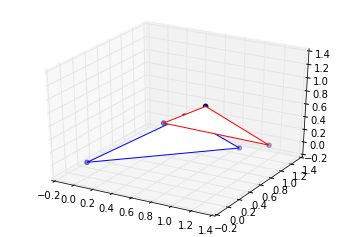
\includegraphics[width=0.95\linewidth,height=0.7\textheight,keepaspectratio]{02_CT_Python_training-chinese_files/02_CT_Python_training-chinese_306_0} \end{center}

\subsection{Reference}\label{reference}

\begin{itemize}
\tightlist
\item
  \url{http://www.byteofpython.info/}
\item
  \url{http://woodpecker.org.cn/abyteofpython_cn/chinese/index.html}
\item
  \url{http://www.python-course.eu/}
\item
  \url{http://ocw.mit.edu/courses/electrical-engineering-and-computer-science/6-189-a-gentle-introduction-to-programming-using-python-january-iap-2008/}
\item
  \url{http://my.oschina.net/taogang/blog/286954}
\end{itemize}

\section{Python作图}\label{Pythonux5fplotux5fWXN}

\subsection{绘图基础}

\subsubsection{Figure和Subplot}\label{figuresubplot-1}

\begin{Shaded}
\begin{Highlighting}[]
\ImportTok{import} \NormalTok{matplotlib.pyplot }\ImportTok{as} \NormalTok{plt}
\ImportTok{import} \NormalTok{numpy }\ImportTok{as} \NormalTok{np}
\ImportTok{import} \NormalTok{pandas }\ImportTok{as} \NormalTok{pd}
\ImportTok{from} \NormalTok{numpy.random }\ImportTok{import} \NormalTok{randn}
\end{Highlighting}
\end{Shaded}

\begin{Shaded}
\begin{Highlighting}[]
\NormalTok{x }\OperatorTok{=} \NormalTok{[}\DecValTok{1}\NormalTok{, }\DecValTok{3}\NormalTok{, }\DecValTok{5}\NormalTok{, }\DecValTok{7}\NormalTok{, }\DecValTok{9}\NormalTok{, }\DecValTok{10}\NormalTok{, }\DecValTok{23}\NormalTok{, }\DecValTok{45}\NormalTok{, }\DecValTok{45}\NormalTok{, }\DecValTok{56}\NormalTok{]}
\NormalTok{y }\OperatorTok{=} \NormalTok{[}\DecValTok{2}\NormalTok{, }\DecValTok{4}\NormalTok{, }\DecValTok{6}\NormalTok{, }\DecValTok{8}\NormalTok{, }\DecValTok{11}\NormalTok{, }\DecValTok{12}\NormalTok{, }\DecValTok{23}\NormalTok{, }\DecValTok{45}\NormalTok{, }\DecValTok{56}\NormalTok{, }\DecValTok{78}\NormalTok{]}


\NormalTok{fig }\OperatorTok{=} \NormalTok{plt.figure()  }\CommentTok{# 创建一个Figure}
\NormalTok{ax1 }\OperatorTok{=} \NormalTok{fig.add_subplot(}\DecValTok{2}\NormalTok{, }\DecValTok{2}\NormalTok{, }\DecValTok{1}\NormalTok{)  }\CommentTok{# 创建4个图的Figure对象,最后的1为选中第一个}
\NormalTok{ax2 }\OperatorTok{=} \NormalTok{fig.add_subplot(}\DecValTok{2}\NormalTok{, }\DecValTok{2}\NormalTok{, }\DecValTok{2}\NormalTok{)}
\NormalTok{ax3 }\OperatorTok{=} \NormalTok{fig.add_subplot(}\DecValTok{2}\NormalTok{, }\DecValTok{2}\NormalTok{, }\DecValTok{3}\NormalTok{)}
\NormalTok{ax4 }\OperatorTok{=} \NormalTok{fig.add_subplot(}\DecValTok{2}\NormalTok{, }\DecValTok{2}\NormalTok{, }\DecValTok{4}\NormalTok{)}

\NormalTok{ax1.hist(x, y)  }\CommentTok{# 在第一图中绘制直方图}
\NormalTok{ax2.scatter(x, y)  }\CommentTok{# 散点图}
\NormalTok{ax4.plot(x, y)  }\CommentTok{# 线图}

\NormalTok{plt.show()}
\end{Highlighting}
\end{Shaded}

\begin{center}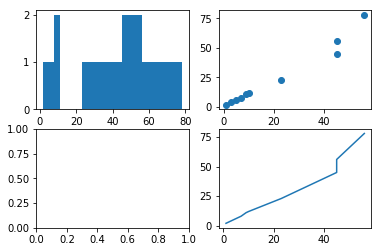
\includegraphics[width=0.95\linewidth,height=0.7\textheight,keepaspectratio]{03_WXN_matplotlib_files/03_WXN_matplotlib_4_0} \end{center}

\begin{Shaded}
\begin{Highlighting}[]
\NormalTok{fig, axes }\OperatorTok{=} \NormalTok{plt.subplots(}\DecValTok{2}\NormalTok{, }\DecValTok{3}\NormalTok{)  }\CommentTok{# 创建一个Figure 绘制2 X3 图}
\NormalTok{fig}
\end{Highlighting}
\end{Shaded}

\begin{center}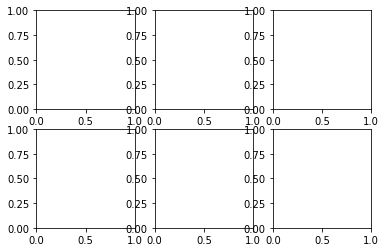
\includegraphics[width=0.95\linewidth,height=0.7\textheight,keepaspectratio]{03_WXN_matplotlib_files/03_WXN_matplotlib_5_0} \end{center}

\begin{Shaded}
\begin{Highlighting}[]
\NormalTok{axes}
\end{Highlighting}
\end{Shaded}

\begin{verbatim}
array([[<matplotlib.axes._subplots.AxesSubplot object at 0x7f8436a71780>,
        <matplotlib.axes._subplots.AxesSubplot object at 0x7f842f2438d0>,
        <matplotlib.axes._subplots.AxesSubplot object at 0x7f842f27d9e8>],
       [<matplotlib.axes._subplots.AxesSubplot object at 0x7f842f236978>,
        <matplotlib.axes._subplots.AxesSubplot object at 0x7f842f1f19b0>,
        <matplotlib.axes._subplots.AxesSubplot object at 0x7f842f199710>]], dtype=object)
\end{verbatim}

\texttt{创建2\ X\ 3图像,可以相当于对二维数组进行索引\ 参数\ \ \ \ \ \ \ \ \ \ \ \ 说明\ nrows\ \ \ \ \ \ \ \ \ \ \ subplot行数\ ncols\ \ \ \ \ \ \ \ \ \ \ subplot列数\ sharex\ \ \ \ \ \ \ \ \ \ 所有图使用相同的x轴\ sharey\ \ \ \ \ \ \ \ \ \ 所有图使用相同的y轴\ subplot\_kw\ \ \ \ \ \ 用于创建各subplot的关键字字典}\textbar{}

\subsubsection{调整subplot周围间距}\label{subplot-1}

\begin{verbatim}
subplots_ajust(left=None,bottom=None,right=None,top=None,wspace=None,hspace=None)
wspace和hspace控制宽度和高度
\end{verbatim}

\begin{Shaded}
\begin{Highlighting}[]
\NormalTok{fig, axes }\OperatorTok{=} \NormalTok{plt.subplots(}\DecValTok{2}\NormalTok{, }\DecValTok{2}\NormalTok{, sharex}\OperatorTok{=}\VariableTok{True}\NormalTok{, sharey}\OperatorTok{=}\VariableTok{True}\NormalTok{)}
\ControlFlowTok{for} \NormalTok{i }\OperatorTok{in} \BuiltInTok{range}\NormalTok{(}\DecValTok{2}\NormalTok{):}
    \ControlFlowTok{for} \NormalTok{j }\OperatorTok{in} \BuiltInTok{range}\NormalTok{(}\DecValTok{2}\NormalTok{):}
        \NormalTok{axes[i, j].hist(randn(}\DecValTok{500}\NormalTok{), bins}\OperatorTok{=}\DecValTok{50}\NormalTok{, color}\OperatorTok{=}\StringTok{'k'}\NormalTok{, alpha}\OperatorTok{=}\FloatTok{0.5}\NormalTok{)}
\NormalTok{plt.subplots_adjust(wspace}\OperatorTok{=}\DecValTok{0}\NormalTok{, hspace}\OperatorTok{=}\DecValTok{0}\NormalTok{)}
\NormalTok{plt.show()}
\end{Highlighting}
\end{Shaded}

\begin{center}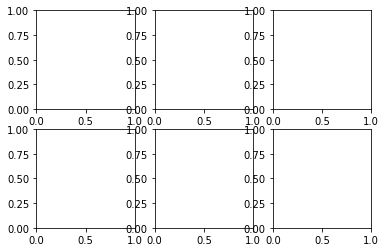
\includegraphics[width=0.95\linewidth,height=0.7\textheight,keepaspectratio]{03_WXN_matplotlib_files/03_WXN_matplotlib_9_0} \end{center}

\begin{center}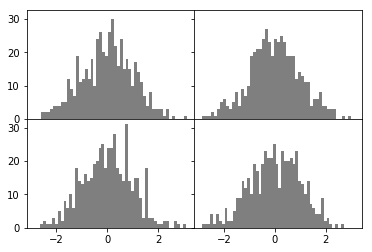
\includegraphics[width=0.95\linewidth,height=0.7\textheight,keepaspectratio]{03_WXN_matplotlib_files/03_WXN_matplotlib_9_1} \end{center}

\begin{Shaded}
\begin{Highlighting}[]
\NormalTok{fig, axes }\OperatorTok{=} \NormalTok{plt.subplots(}\DecValTok{2}\NormalTok{, }\DecValTok{2}\NormalTok{, sharex}\OperatorTok{=}\VariableTok{True}\NormalTok{, sharey}\OperatorTok{=}\VariableTok{True}\NormalTok{)}
\ControlFlowTok{for} \NormalTok{i }\OperatorTok{in} \BuiltInTok{range}\NormalTok{(}\DecValTok{2}\NormalTok{):}
    \ControlFlowTok{for} \NormalTok{j }\OperatorTok{in} \BuiltInTok{range}\NormalTok{(}\DecValTok{2}\NormalTok{):}
        \NormalTok{axes[i, j].hist(randn(}\DecValTok{500}\NormalTok{), bins}\OperatorTok{=}\DecValTok{50}\NormalTok{, color}\OperatorTok{=}\StringTok{'k'}\NormalTok{, alpha}\OperatorTok{=}\FloatTok{0.5}\NormalTok{)}
\NormalTok{plt.subplots_adjust(wspace}\OperatorTok{=}\DecValTok{2}\NormalTok{, hspace}\OperatorTok{=}\FloatTok{0.5}\NormalTok{)}
\NormalTok{plt.show()}
\end{Highlighting}
\end{Shaded}

\begin{center}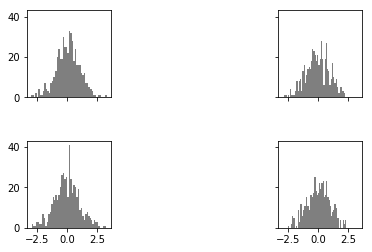
\includegraphics[width=0.95\linewidth,height=0.7\textheight,keepaspectratio]{03_WXN_matplotlib_files/03_WXN_matplotlib_10_0} \end{center}

\begin{Shaded}
\begin{Highlighting}[]
\NormalTok{fig}
\end{Highlighting}
\end{Shaded}

\begin{center}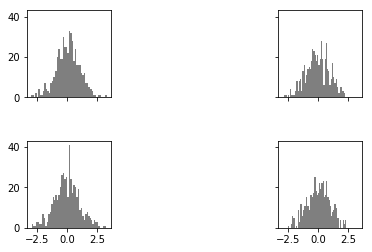
\includegraphics[width=0.95\linewidth,height=0.7\textheight,keepaspectratio]{03_WXN_matplotlib_files/03_WXN_matplotlib_11_0} \end{center}

\subsubsection{颜色 标记和线型}\label{--1}

\begin{Shaded}
\begin{Highlighting}[]
\CommentTok{"""}
\CommentTok{绘制绿色虚线}
\CommentTok{ax.plot(x,y,'g--')}
\CommentTok{另一种方式}
\CommentTok{ax.plot(x,y,linestyle='--',color='g')}
\CommentTok{标记点(maker)}
\CommentTok{"""}
\NormalTok{fig, axes }\OperatorTok{=} \NormalTok{plt.subplots(}\DecValTok{1}\NormalTok{, }\DecValTok{2}\NormalTok{)}

\NormalTok{axes[}\DecValTok{0}\NormalTok{].plot(randn(}\DecValTok{10}\NormalTok{), }\StringTok{'g--'}\NormalTok{)  }\CommentTok{# green ---}
\NormalTok{axes[}\DecValTok{1}\NormalTok{].plot(randn(}\DecValTok{10}\NormalTok{), }\StringTok{'ko--'}\NormalTok{)  }\CommentTok{# k:black o:圆点}

\NormalTok{plt.show()}
\end{Highlighting}
\end{Shaded}

\begin{center}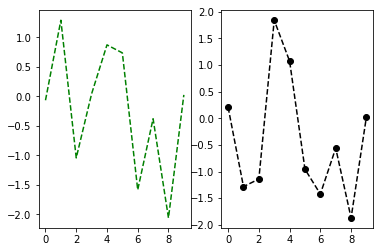
\includegraphics[width=0.95\linewidth,height=0.7\textheight,keepaspectratio]{03_WXN_matplotlib_files/03_WXN_matplotlib_13_0} \end{center}

\begin{verbatim}
character   description
'-' solid line style
'--'    dashed line style
'-.'    dash-dot line style
':' dotted line style
'.' point marker
',' pixel marker
'o' circle marker
'v' triangle_down marker
'^' triangle_up marker
'<' triangle_left marker
'>' triangle_right marker
'1' tri_down marker
'2' tri_up marker
'3' tri_left marker
'4' tri_right marker
's' square marker
'p' pentagon marker
'*' star marker
'h' hexagon1 marker
'H' hexagon2 marker
'+' plus marker
'x' x marker
'D' diamond marker
'd' thin_diamond marker
'|' vline marker
'_' hline marker

The following color abbreviations are supported:

character   color
‘b’ blue
‘g’ green
‘r’ red
‘c’ cyan(青色)
‘m’ magenta(紫红色)
‘y’ yellow
‘k’ black
‘w’ white

https://matplotlib.org/api/_as_gen/matplotlib.pyplot.plot.html#matplotlib.pyplot.plot
\end{verbatim}

\subsubsection{刻度、标签和图例}\label{-1}

\begin{Shaded}
\begin{Highlighting}[]
\NormalTok{fig }\OperatorTok{=} \NormalTok{plt.figure()  }\CommentTok{# 创建一个Figure}
\NormalTok{ax }\OperatorTok{=} \NormalTok{fig.add_subplot(}\DecValTok{1}\NormalTok{, }\DecValTok{1}\NormalTok{, }\DecValTok{1}\NormalTok{)}
\NormalTok{ax.plot(randn(}\DecValTok{100}\NormalTok{))}
\NormalTok{plt.show()}
\end{Highlighting}
\end{Shaded}

\begin{center}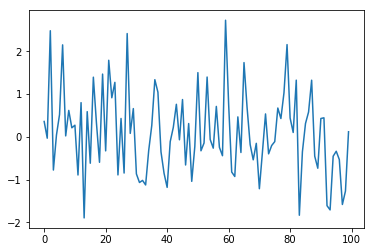
\includegraphics[width=0.95\linewidth,height=0.7\textheight,keepaspectratio]{03_WXN_matplotlib_files/03_WXN_matplotlib_16_0} \end{center}

\begin{Shaded}
\begin{Highlighting}[]
\CommentTok{"""修改上图的轴"""}

\NormalTok{fig }\OperatorTok{=} \NormalTok{plt.figure()}
\NormalTok{ax }\OperatorTok{=} \NormalTok{fig.add_subplot(}\DecValTok{1}\NormalTok{, }\DecValTok{1}\NormalTok{, }\DecValTok{1}\NormalTok{)}
\NormalTok{ax.plot(randn(}\DecValTok{100}\NormalTok{))}

\NormalTok{ticks }\OperatorTok{=} \NormalTok{ax.set_xticks([}\DecValTok{0}\NormalTok{, }\DecValTok{25}\NormalTok{, }\DecValTok{50}\NormalTok{, }\DecValTok{75}\NormalTok{, }\DecValTok{100}\NormalTok{])  }\CommentTok{# 设置刻度}
\NormalTok{labels }\OperatorTok{=} \NormalTok{ax.set_xticklabels(}
    \NormalTok{[}\StringTok{'first'}\NormalTok{, }\StringTok{'second'}\NormalTok{, }\StringTok{'third'}\NormalTok{, }\StringTok{'forth'}\NormalTok{, }\StringTok{'fifth'}\NormalTok{], rotation}\OperatorTok{=}\DecValTok{30}\NormalTok{, fontsize}\OperatorTok{=}\StringTok{'small'}\NormalTok{)  }\CommentTok{# 设置x轴标签}

\NormalTok{ax.set_title(}\StringTok{'my first matplot plot'}\NormalTok{)  }\CommentTok{# 设置图片标题}

\NormalTok{ax.set_xlabel(}\StringTok{'Stages'}\NormalTok{)  }\CommentTok{# 设置x轴名称}

\NormalTok{plt.show()}
\end{Highlighting}
\end{Shaded}

\begin{center}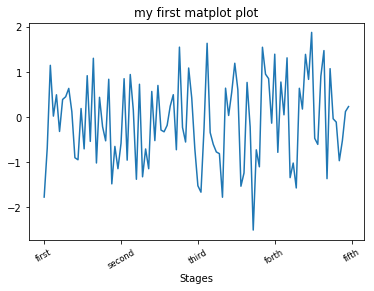
\includegraphics[width=0.95\linewidth,height=0.7\textheight,keepaspectratio]{03_WXN_matplotlib_files/03_WXN_matplotlib_17_0} \end{center}

\subsubsection{添加图例legend}\label{legend-1}

\begin{verbatim}
https://matplotlib.org/api/legend_api.html?highlight=legend#module-matplotlib.legend
‘best’          0
‘upper right’   1
‘upper left’    2
‘lower left’    3
‘lower right’   4
‘right’         5
‘center left’   6
‘center right’  7
‘lower center’  8
‘upper center’  9
‘center’        10
bbox_to_anchor=(0.5,0.8)
bbox_to_anchor被赋予的元组中,第一个数值用于控制legend的左右移动,值越大越向右边移动,
第二个数值用于控制legend的上下移动,值越大,越向上移动
\end{verbatim}

\begin{Shaded}
\begin{Highlighting}[]
\NormalTok{fig }\OperatorTok{=} \NormalTok{plt.figure()}
\NormalTok{ax }\OperatorTok{=} \NormalTok{fig.add_subplot(}\DecValTok{1}\NormalTok{, }\DecValTok{1}\NormalTok{, }\DecValTok{1}\NormalTok{)}

\NormalTok{ax.plot(randn(}\DecValTok{10}\NormalTok{), }\StringTok{'k'}\NormalTok{, label}\OperatorTok{=}\StringTok{'one'}\NormalTok{)  }\CommentTok{# 画一条线,k黑色}
\NormalTok{ax.plot(randn(}\DecValTok{10}\NormalTok{), }\StringTok{'g--'}\NormalTok{, label}\OperatorTok{=}\StringTok{'two'}\NormalTok{)  }\CommentTok{# 画第二条线,g绿色 - -类型}
\NormalTok{ax.plot(randn(}\DecValTok{10}\NormalTok{), }\StringTok{'ro--'}\NormalTok{, label}\OperatorTok{=}\StringTok{'three'}\NormalTok{)  }\CommentTok{# 画第三条线红色 ,类型 ...}

\NormalTok{ax.legend(loc}\OperatorTok{=}\DecValTok{0}\NormalTok{, bbox_to_anchor}\OperatorTok{=}\NormalTok{(}\DecValTok{1}\NormalTok{, }\DecValTok{1}\NormalTok{))}


\NormalTok{plt.show()}
\end{Highlighting}
\end{Shaded}

\begin{center}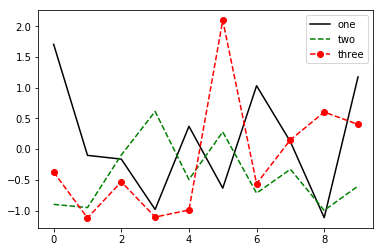
\includegraphics[width=0.95\linewidth,height=0.7\textheight,keepaspectratio]{03_WXN_matplotlib_files/03_WXN_matplotlib_19_0} \end{center}

\subsubsection{注解}\label{-1}

\begin{Shaded}
\begin{Highlighting}[]
\NormalTok{x }\OperatorTok{=} \NormalTok{[}\DecValTok{2}\NormalTok{, }\DecValTok{4}\NormalTok{, }\DecValTok{6}\NormalTok{, }\DecValTok{8}\NormalTok{, }\DecValTok{10}\NormalTok{, }\DecValTok{12}\NormalTok{]}
\NormalTok{y }\OperatorTok{=} \NormalTok{[}\DecValTok{1}\NormalTok{, }\DecValTok{3}\NormalTok{, }\DecValTok{5}\NormalTok{, }\DecValTok{7}\NormalTok{, }\DecValTok{9}\NormalTok{, }\DecValTok{11}\NormalTok{]}
\NormalTok{fig }\OperatorTok{=} \NormalTok{plt.figure()}
\NormalTok{ax }\OperatorTok{=} \NormalTok{fig.add_subplot(}\DecValTok{1}\NormalTok{, }\DecValTok{1}\NormalTok{, }\DecValTok{1}\NormalTok{)}
\NormalTok{ax.plot(x, y, }\StringTok{'r--'}\NormalTok{)}

\NormalTok{ax.text(}\DecValTok{2}\NormalTok{, }\DecValTok{4}\NormalTok{, }\StringTok{'hello python'}\NormalTok{)}
\NormalTok{plt.show()}
\end{Highlighting}
\end{Shaded}

\begin{center}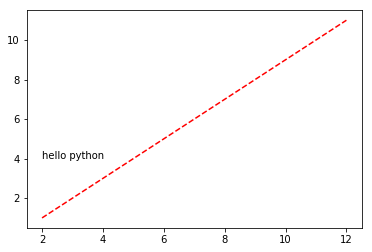
\includegraphics[width=0.95\linewidth,height=0.7\textheight,keepaspectratio]{03_WXN_matplotlib_files/03_WXN_matplotlib_21_0} \end{center}

\begin{Shaded}
\begin{Highlighting}[]
\NormalTok{ax }\OperatorTok{=} \NormalTok{plt.subplot(}\DecValTok{111}\NormalTok{)}

\NormalTok{t }\OperatorTok{=} \NormalTok{np.arange(}\FloatTok{0.0}\NormalTok{, }\FloatTok{5.0}\NormalTok{, }\FloatTok{0.01}\NormalTok{)}
\NormalTok{s }\OperatorTok{=} \NormalTok{np.cos(}\DecValTok{2} \OperatorTok{*} \NormalTok{np.pi }\OperatorTok{*} \NormalTok{t)}
\NormalTok{line, }\OperatorTok{=} \NormalTok{plt.plot(t, s, lw}\OperatorTok{=}\DecValTok{2}\NormalTok{)}

\NormalTok{plt.annotate(}\StringTok{'local max'}\NormalTok{, xy}\OperatorTok{=}\NormalTok{(}\DecValTok{2}\NormalTok{, }\DecValTok{1}\NormalTok{), xytext}\OperatorTok{=}\NormalTok{(}\DecValTok{3}\NormalTok{, }\FloatTok{1.5}\NormalTok{),}
             \NormalTok{arrowprops}\OperatorTok{=}\BuiltInTok{dict}\NormalTok{(facecolor}\OperatorTok{=}\StringTok{'blue'}\NormalTok{)  }\CommentTok{# xy=(要注释的点),xytext=(注释在图中的位置)}
             \NormalTok{)}

\NormalTok{plt.ylim(}\OperatorTok{-}\DecValTok{2}\NormalTok{, }\DecValTok{2}\NormalTok{)}
\NormalTok{plt.show()}
\end{Highlighting}
\end{Shaded}

\begin{center}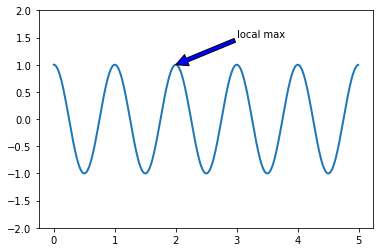
\includegraphics[width=0.95\linewidth,height=0.7\textheight,keepaspectratio]{03_WXN_matplotlib_files/03_WXN_matplotlib_22_0} \end{center}

\subsubsection{图片保存}\label{-1}

\begin{Shaded}
\begin{Highlighting}[]
\NormalTok{x }\OperatorTok{=} \NormalTok{[}\DecValTok{2}\NormalTok{, }\DecValTok{4}\NormalTok{, }\DecValTok{6}\NormalTok{, }\DecValTok{8}\NormalTok{, }\DecValTok{10}\NormalTok{, }\DecValTok{12}\NormalTok{]}
\NormalTok{y }\OperatorTok{=} \NormalTok{[}\DecValTok{1}\NormalTok{, }\DecValTok{3}\NormalTok{, }\DecValTok{5}\NormalTok{, }\DecValTok{7}\NormalTok{, }\DecValTok{9}\NormalTok{, }\DecValTok{11}\NormalTok{]}
\NormalTok{fig }\OperatorTok{=} \NormalTok{plt.figure()}
\NormalTok{ax }\OperatorTok{=} \NormalTok{fig.add_subplot(}\DecValTok{1}\NormalTok{, }\DecValTok{1}\NormalTok{, }\DecValTok{1}\NormalTok{)}
\NormalTok{ax.plot(x, y, }\StringTok{'r--'}\NormalTok{)}

\NormalTok{ax.text(}\DecValTok{2}\NormalTok{, }\DecValTok{4}\NormalTok{, }\StringTok{'hello python'}\NormalTok{)}

\CommentTok{# bbox_inches减除当前图片周围空白部分}
\NormalTok{plt.savefig(}\StringTok{'figpath.jpg'}\NormalTok{, dpi}\OperatorTok{=}\DecValTok{300}\NormalTok{, bbox_inches}\OperatorTok{=}\StringTok{'tight'}\NormalTok{)}
\end{Highlighting}
\end{Shaded}

\subsection{绘图实例}

\subsubsection{绘制散点图}\label{-1}

\begin{Shaded}
\begin{Highlighting}[]
\NormalTok{x }\OperatorTok{=} \NormalTok{[}\DecValTok{1}\NormalTok{, }\DecValTok{2}\NormalTok{, }\DecValTok{3}\NormalTok{, }\DecValTok{4}\NormalTok{, }\DecValTok{5}\NormalTok{, }\DecValTok{6}\NormalTok{]}
\NormalTok{y }\OperatorTok{=} \NormalTok{[}\DecValTok{1}\NormalTok{, }\DecValTok{4}\NormalTok{, }\DecValTok{9}\NormalTok{, }\DecValTok{16}\NormalTok{, }\DecValTok{25}\NormalTok{, }\DecValTok{36}\NormalTok{]}
\NormalTok{plt.scatter(x,  }\CommentTok{# x轴数据}
            \NormalTok{y,  }\CommentTok{# y轴数据}
            \NormalTok{s}\OperatorTok{=}\DecValTok{20}\NormalTok{,  }\CommentTok{# 设置点的大小}
            \NormalTok{c}\OperatorTok{=}\StringTok{'green'}\NormalTok{,  }\CommentTok{# 设置点的颜色}
            \NormalTok{marker}\OperatorTok{=}\StringTok{'s'}\NormalTok{,  }\CommentTok{# 设置点的形状}
            \NormalTok{alpha}\OperatorTok{=}\FloatTok{0.9}\NormalTok{,  }\CommentTok{# 设置点的透明度}
            \NormalTok{linewidths}\OperatorTok{=}\FloatTok{0.8}\NormalTok{,  }\CommentTok{# 设置散点边界的粗细}
            \NormalTok{edgecolors}\OperatorTok{=}\StringTok{'red'}  \CommentTok{# 设置散点边界的颜色}
            \NormalTok{)}

\NormalTok{plt.title(}\StringTok{'simple scatter plot'}\NormalTok{)}
\NormalTok{plt.xlabel(}\StringTok{'X'}\NormalTok{)  }\CommentTok{# x轴名称}
\NormalTok{plt.ylabel(}\StringTok{'Y'}\NormalTok{)}

\NormalTok{plt.show()  }\CommentTok{# 展示绘图}
\end{Highlighting}
\end{Shaded}

\begin{center}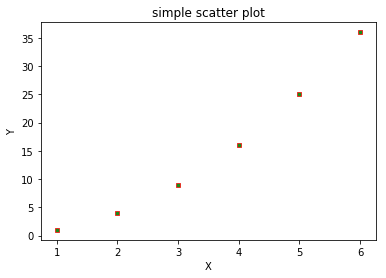
\includegraphics[width=0.95\linewidth,height=0.7\textheight,keepaspectratio]{03_WXN_matplotlib_files/03_WXN_matplotlib_27_0} \end{center}

\subsubsection{折线图}\label{-1}

\begin{Shaded}
\begin{Highlighting}[]
\NormalTok{x }\OperatorTok{=} \NormalTok{[}\DecValTok{1}\NormalTok{, }\DecValTok{2}\NormalTok{, }\DecValTok{3}\NormalTok{, }\DecValTok{4}\NormalTok{, }\DecValTok{5}\NormalTok{, }\DecValTok{6}\NormalTok{]}
\NormalTok{y }\OperatorTok{=} \NormalTok{[}\DecValTok{1}\NormalTok{, }\DecValTok{4}\NormalTok{, }\DecValTok{9}\NormalTok{, }\DecValTok{16}\NormalTok{, }\DecValTok{25}\NormalTok{, }\DecValTok{36}\NormalTok{]}

\NormalTok{plt.plot(x,  }\CommentTok{# x轴数据}
         \NormalTok{y,  }\CommentTok{# y轴数据}
         \NormalTok{linestyle}\OperatorTok{=}\StringTok{'-'}\NormalTok{,  }\CommentTok{# 折线类型}
         \NormalTok{linewidth}\OperatorTok{=}\DecValTok{2}\NormalTok{,  }\CommentTok{# 折线宽度}
         \NormalTok{color}\OperatorTok{=}\StringTok{'blue'}\NormalTok{,  }\CommentTok{# 折线颜色}
         \NormalTok{marker}\OperatorTok{=}\StringTok{'o'}\NormalTok{,  }\CommentTok{# 点的形状}
         \NormalTok{markersize}\OperatorTok{=}\DecValTok{8}\NormalTok{,  }\CommentTok{# 点的大小}
         \NormalTok{markeredgecolor}\OperatorTok{=}\StringTok{'black'}\NormalTok{,  }\CommentTok{# 点的边框色}
         \NormalTok{markerfacecolor}\OperatorTok{=}\StringTok{'red'}\NormalTok{)  }\CommentTok{# 点的填充色}


\CommentTok{# 添加标题和坐标轴标签}
\NormalTok{plt.title(}\StringTok{'line plot'}\NormalTok{)}
\NormalTok{plt.xlabel(}\StringTok{'X'}\NormalTok{)}
\NormalTok{plt.ylabel(}\StringTok{'Y'}\NormalTok{)}

\NormalTok{plt.show()}
\end{Highlighting}
\end{Shaded}

\begin{center}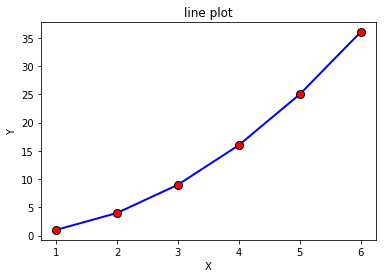
\includegraphics[width=0.95\linewidth,height=0.7\textheight,keepaspectratio]{03_WXN_matplotlib_files/03_WXN_matplotlib_29_0} \end{center}

\begin{Shaded}
\begin{Highlighting}[]
\ImportTok{import} \NormalTok{numpy }\ImportTok{as} \NormalTok{np}
\ImportTok{import} \NormalTok{matplotlib.pyplot }\ImportTok{as} \NormalTok{plt}


\NormalTok{t }\OperatorTok{=} \NormalTok{np.arange(}\DecValTok{0}\NormalTok{., }\DecValTok{5}\NormalTok{., }\FloatTok{0.2}\NormalTok{)}

\NormalTok{t}
\end{Highlighting}
\end{Shaded}

\begin{verbatim}
array([ 0. ,  0.2,  0.4,  0.6,  0.8,  1. ,  1.2,  1.4,  1.6,  1.8,  2. ,
        2.2,  2.4,  2.6,  2.8,  3. ,  3.2,  3.4,  3.6,  3.8,  4. ,  4.2,
        4.4,  4.6,  4.8])
\end{verbatim}

\begin{Shaded}
\begin{Highlighting}[]
\CommentTok{# red dashes, blue squares and green triangles}
\NormalTok{plt.plot(t, t, }\StringTok{'r--'}\NormalTok{, t, t}\OperatorTok{**}\DecValTok{2}\NormalTok{, }\StringTok{'bs'}\NormalTok{, t, t}\OperatorTok{**}\DecValTok{3}\NormalTok{, }\StringTok{'g'}\NormalTok{)}
\NormalTok{plt.show()}
\end{Highlighting}
\end{Shaded}

\begin{center}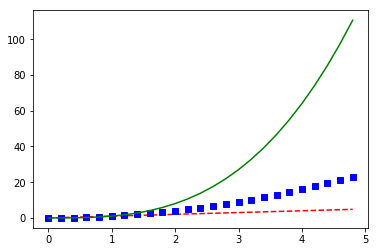
\includegraphics[width=0.95\linewidth,height=0.7\textheight,keepaspectratio]{03_WXN_matplotlib_files/03_WXN_matplotlib_31_0} \end{center}

\begin{Shaded}
\begin{Highlighting}[]
\CommentTok{# 同一效果}
\NormalTok{fig }\OperatorTok{=} \NormalTok{plt.figure()}
\NormalTok{ax }\OperatorTok{=} \NormalTok{fig.add_subplot(}\DecValTok{1}\NormalTok{, }\DecValTok{1}\NormalTok{, }\DecValTok{1}\NormalTok{)}
\NormalTok{ax.plot(t, t, }\StringTok{'r--'}\NormalTok{)}
\NormalTok{ax.plot(t, t}\OperatorTok{**}\DecValTok{2}\NormalTok{, }\StringTok{'bs'}\NormalTok{)  }\CommentTok{# 'bs'表示blue square marker}
\NormalTok{ax.plot(t, t}\OperatorTok{**}\DecValTok{3}\NormalTok{, }\StringTok{'g'}\NormalTok{)}
\NormalTok{fig}
\end{Highlighting}
\end{Shaded}

\begin{center}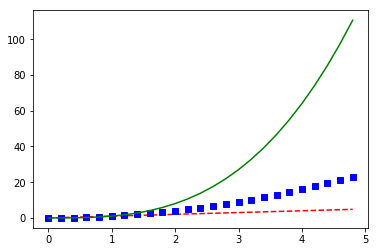
\includegraphics[width=0.95\linewidth,height=0.7\textheight,keepaspectratio]{03_WXN_matplotlib_files/03_WXN_matplotlib_32_0} \end{center}

\subsubsection{直方图}\label{-1}

\begin{Shaded}
\begin{Highlighting}[]
\ImportTok{import} \NormalTok{numpy }\ImportTok{as} \NormalTok{np}
\ImportTok{import} \NormalTok{pandas }\ImportTok{as} \NormalTok{pd}
\ImportTok{import} \NormalTok{matplotlib.pyplot }\ImportTok{as} \NormalTok{plt}

\NormalTok{plt.hist(np.random.randn(}\DecValTok{50}\NormalTok{),  }\CommentTok{# 绘图数据}
         \NormalTok{bins}\OperatorTok{=}\DecValTok{50}\NormalTok{,  }\CommentTok{# 指定直方图的条形数}
         \NormalTok{color}\OperatorTok{=}\StringTok{'red'}\NormalTok{,  }\CommentTok{# 指定填充色}
         \NormalTok{edgecolor}\OperatorTok{=}\StringTok{'k'}\NormalTok{)  }\CommentTok{# 指定直方图的边界色k :black}
\NormalTok{plt.show()}
\end{Highlighting}
\end{Shaded}

\begin{center}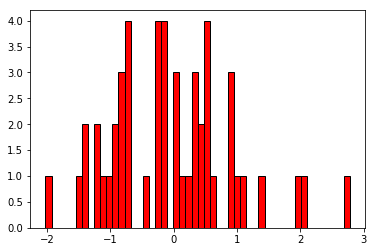
\includegraphics[width=0.95\linewidth,height=0.7\textheight,keepaspectratio]{03_WXN_matplotlib_files/03_WXN_matplotlib_34_0} \end{center}

\subsubsection{直条图}\label{-1}

\begin{Shaded}
\begin{Highlighting}[]
\NormalTok{x }\OperatorTok{=} \NormalTok{[}\DecValTok{1}\NormalTok{, }\DecValTok{2}\NormalTok{, }\DecValTok{3}\NormalTok{, }\DecValTok{4}\NormalTok{, }\DecValTok{5}\NormalTok{, }\DecValTok{6}\NormalTok{]}
\NormalTok{y }\OperatorTok{=} \NormalTok{[}\DecValTok{1}\NormalTok{, }\DecValTok{4}\NormalTok{, }\DecValTok{9}\NormalTok{, }\DecValTok{16}\NormalTok{, }\DecValTok{25}\NormalTok{, }\DecValTok{36}\NormalTok{]}

\NormalTok{plt.bar(x, y,}
        \NormalTok{color}\OperatorTok{=}\StringTok{'steelblue'}\NormalTok{,}
        \NormalTok{alpha}\OperatorTok{=}\FloatTok{0.8}\NormalTok{)}

\NormalTok{plt.title(}\StringTok{'bar plot'}\NormalTok{)}

\NormalTok{plt.ylim([}\DecValTok{0}\NormalTok{, }\DecValTok{40}\NormalTok{])}
\NormalTok{plt.show()}
\end{Highlighting}
\end{Shaded}

\begin{center}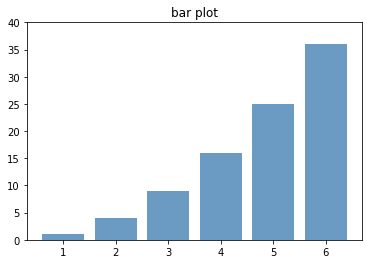
\includegraphics[width=0.95\linewidth,height=0.7\textheight,keepaspectratio]{03_WXN_matplotlib_files/03_WXN_matplotlib_36_0} \end{center}

\begin{Shaded}
\begin{Highlighting}[]
\NormalTok{x }\OperatorTok{=} \NormalTok{[}\DecValTok{1}\NormalTok{, }\DecValTok{2}\NormalTok{, }\DecValTok{3}\NormalTok{, }\DecValTok{4}\NormalTok{, }\DecValTok{5}\NormalTok{, }\DecValTok{6}\NormalTok{]}
\NormalTok{y }\OperatorTok{=} \NormalTok{[}\DecValTok{1}\NormalTok{, }\DecValTok{4}\NormalTok{, }\DecValTok{9}\NormalTok{, }\DecValTok{16}\NormalTok{, }\DecValTok{25}\NormalTok{, }\DecValTok{36}\NormalTok{]}

\NormalTok{plt.barh(x, y,}
         \NormalTok{color}\OperatorTok{=}\StringTok{'steelblue'}\NormalTok{,}
         \NormalTok{alpha}\OperatorTok{=}\FloatTok{0.8}\NormalTok{)}

\NormalTok{plt.title(}\StringTok{'bar plot'}\NormalTok{)}

\NormalTok{plt.show()}
\end{Highlighting}
\end{Shaded}

\begin{center}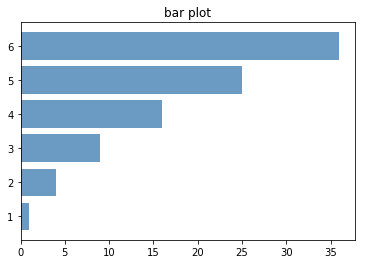
\includegraphics[width=0.95\linewidth,height=0.7\textheight,keepaspectratio]{03_WXN_matplotlib_files/03_WXN_matplotlib_37_0} \end{center}

\subsubsection{箱线图}\label{-1}

\begin{Shaded}
\begin{Highlighting}[]
\NormalTok{x }\OperatorTok{=} \NormalTok{[}\DecValTok{1}\NormalTok{, }\DecValTok{2}\NormalTok{, }\DecValTok{3}\NormalTok{, }\DecValTok{4}\NormalTok{, }\DecValTok{5}\NormalTok{, }\DecValTok{6}\NormalTok{]}
\NormalTok{plt.boxplot(x,}
            \NormalTok{patch_artist}\OperatorTok{=}\VariableTok{True}\NormalTok{,  }\CommentTok{# 箱体添加颜色}
            \NormalTok{labels}\OperatorTok{=}\NormalTok{[}\StringTok{'boxplot'}\NormalTok{],  }\CommentTok{# 添加具体的标签名称}
            \NormalTok{showmeans}\OperatorTok{=}\VariableTok{True}\NormalTok{)}

\CommentTok{# 显示图形}
\NormalTok{plt.show()}
\end{Highlighting}
\end{Shaded}

\begin{center}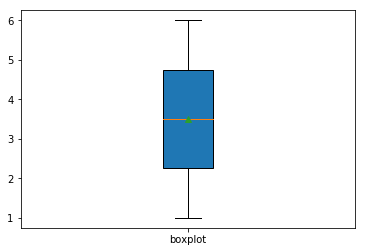
\includegraphics[width=0.95\linewidth,height=0.7\textheight,keepaspectratio]{03_WXN_matplotlib_files/03_WXN_matplotlib_39_0} \end{center}

\begin{Shaded}
\begin{Highlighting}[]
\NormalTok{np.random.seed(}\DecValTok{2}\NormalTok{)  }\CommentTok{# 设置随机种子}
\NormalTok{df }\OperatorTok{=} \NormalTok{pd.DataFrame(np.random.rand(}\DecValTok{5}\NormalTok{, }\DecValTok{4}\NormalTok{),}
                  \NormalTok{columns}\OperatorTok{=}\NormalTok{([}\StringTok{'A'}\NormalTok{, }\StringTok{'B'}\NormalTok{, }\StringTok{'C'}\NormalTok{, }\StringTok{'D'}\NormalTok{]))}
\NormalTok{df}
\end{Highlighting}
\end{Shaded}

\begin{verbatim}
<tr style="text-align: right;">
  <th></th>
  <th>A</th>
  <th>B</th>
  <th>C</th>
  <th>D</th>
</tr>
\end{verbatim}

\begin{verbatim}
<tr>
  <th>0</th>
  <td>0.435995</td>
  <td>0.025926</td>
  <td>0.549662</td>
  <td>0.435322</td>
</tr>
<tr>
  <th>1</th>
  <td>0.420368</td>
  <td>0.330335</td>
  <td>0.204649</td>
  <td>0.619271</td>
</tr>
<tr>
  <th>2</th>
  <td>0.299655</td>
  <td>0.266827</td>
  <td>0.621134</td>
  <td>0.529142</td>
</tr>
<tr>
  <th>3</th>
  <td>0.134580</td>
  <td>0.513578</td>
  <td>0.184440</td>
  <td>0.785335</td>
</tr>
<tr>
  <th>4</th>
  <td>0.853975</td>
  <td>0.494237</td>
  <td>0.846561</td>
  <td>0.079645</td>
</tr>
\end{verbatim}

\begin{Shaded}
\begin{Highlighting}[]
\NormalTok{data }\OperatorTok{=} \NormalTok{[]}
\ControlFlowTok{for} \NormalTok{i }\OperatorTok{in} \BuiltInTok{range}\NormalTok{(}\DecValTok{4}\NormalTok{):}
    \NormalTok{data.append(df.iloc[:, i])}
\NormalTok{data}
\end{Highlighting}
\end{Shaded}

\begin{verbatim}
[0    0.435995
 1    0.420368
 2    0.299655
 3    0.134580
 4    0.853975
 Name: A, dtype: float64, 0    0.025926
 1    0.330335
 2    0.266827
 3    0.513578
 4    0.494237
 Name: B, dtype: float64, 0    0.549662
 1    0.204649
 2    0.621134
 3    0.184440
 4    0.846561
 Name: C, dtype: float64, 0    0.435322
 1    0.619271
 2    0.529142
 3    0.785335
 4    0.079645
 Name: D, dtype: float64]
\end{verbatim}

\begin{Shaded}
\begin{Highlighting}[]
\NormalTok{plt.boxplot(data)}
\NormalTok{plt.show()}
\end{Highlighting}
\end{Shaded}

\begin{center}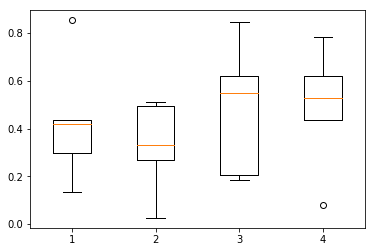
\includegraphics[width=0.95\linewidth,height=0.7\textheight,keepaspectratio]{03_WXN_matplotlib_files/03_WXN_matplotlib_42_0} \end{center}

\begin{verbatim}
plt.boxplot(x, notch=None, sym=None, vert=None, 
             whis=None, positions=None, widths=None, 
             patch_artist=None, meanline=None, showmeans=None, 
             showcaps=None, showbox=None, showfliers=None, 
             boxprops=None, labels=None, flierprops=None, 
             medianprops=None, meanprops=None, 
             capprops=None, whiskerprops=None)

x:指定要绘制箱线图的数据;
notch:是否凹口的形式展现箱线图,默认非凹口;
sym:指定异常点的形状,默认为+号显示;
vert:是否需要将箱线图垂直摆放,默认垂直摆放;
whis:指定上下须与上下四分位的距离,默认为1.5倍的四分位差;
positions:指定箱线图的位置,默认为[0,1,2…];
widths:指定箱线图的宽度,默认为0.5;
patch_artist:是否填充箱体的颜色;
meanline:是否用线的形式表示均值,默认用点来表示;
showmeans:是否显示均值,默认不显示;
showcaps:是否显示箱线图顶端和末端的两条线,默认显示;
showbox:是否显示箱线图的箱体,默认显示;
showfliers:是否显示异常值,默认显示;
boxprops:设置箱体的属性,如边框色,填充色等;
labels:为箱线图添加标签,类似于图例的作用;
filerprops:设置异常值的属性,如异常点的形状、大小、填充色等;
medianprops:设置中位数的属性,如线的类型、粗细等;
meanprops:设置均值的属性,如点的大小、颜色等;
capprops:设置箱线图顶端和末端线条的属性,如颜色、粗细等;
whiskerprops:设置须的属性,如颜色、粗细、线的类型等;
\end{verbatim}

\subsubsection{饼图}\label{-1}

\begin{Shaded}
\begin{Highlighting}[]
\NormalTok{data }\OperatorTok{=} \NormalTok{[}\FloatTok{0.2}\NormalTok{, }\FloatTok{0.3}\NormalTok{, }\FloatTok{0.4}\NormalTok{, }\FloatTok{0.1}\NormalTok{]}
\NormalTok{plt.pie(data)}
\NormalTok{plt.show()}
\end{Highlighting}
\end{Shaded}

\begin{center}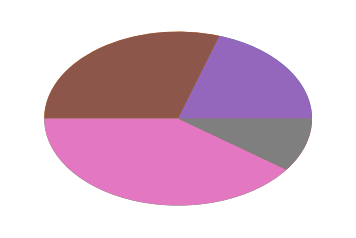
\includegraphics[width=0.95\linewidth,height=0.7\textheight,keepaspectratio]{03_WXN_matplotlib_files/03_WXN_matplotlib_45_0} \end{center}

\begin{verbatim}
plt.pie(x, explode=None, labels=None, colors=None, 
        autopct=None, pctdistance=0.6, shadow=False, 
        labeldistance=1.1, startangle=None, 
        radius=None, counterclock=True, wedgeprops=None, 
        textprops=None, center=(0, 0), frame=False)
        
x:指定绘图的数据;
explode:指定饼图某些部分的突出显示,即呈现爆炸式;
labels:为饼图添加标签说明,类似于图例说明;
colors:指定饼图的填充色;
autopct:自动添加百分比显示,可以采用格式化的方法显示;
pctdistance:设置百分比标签与圆心的距离;
shadow:是否添加饼图的阴影效果;
labeldistance:设置各扇形标签(图例)与圆心的距离;
startangle:设置饼图的初始摆放角度;
radius:设置饼图的半径大小;
counterclock:是否让饼图按逆时针顺序呈现;
wedgeprops:设置饼图内外边界的属性,如边界线的粗细、颜色等;
textprops:设置饼图中文本的属性,如字体大小、颜色等;
center:指定饼图的中心点位置,默认为原点
frame:是否要显示饼图背后的图框,如果设置为True的话,需要同时控制图框x轴、y轴的范围和饼图的中心位置;
\end{verbatim}

\subsubsection{绘制基因矩阵的热图}

\begin{Shaded}
\begin{Highlighting}[]
\CommentTok{# 来源于百度经验}
\ImportTok{import} \NormalTok{numpy }\ImportTok{as} \NormalTok{np}
\ImportTok{from} \NormalTok{matplotlib }\ImportTok{import} \NormalTok{pyplot }\ImportTok{as} \NormalTok{plt}
\ImportTok{from} \NormalTok{matplotlib }\ImportTok{import} \NormalTok{cm}
\ImportTok{from} \NormalTok{matplotlib }\ImportTok{import} \NormalTok{axes}


\KeywordTok{def} \NormalTok{draw_heatmap(data, xlabels, ylabels):  }\CommentTok{# 自定义函数,3个参数}
    \NormalTok{cmap }\OperatorTok{=} \NormalTok{cm.Blues}
    \NormalTok{figure }\OperatorTok{=} \NormalTok{plt.figure(facecolor}\OperatorTok{=}\StringTok{'w'}\NormalTok{)}
    \NormalTok{ax }\OperatorTok{=} \NormalTok{figure.add_subplot(}\DecValTok{1}\NormalTok{, }\DecValTok{1}\NormalTok{, }\DecValTok{1}\NormalTok{, position}\OperatorTok{=}\NormalTok{[}\FloatTok{0.1}\NormalTok{, }\FloatTok{0.15}\NormalTok{, }\FloatTok{0.8}\NormalTok{, }\FloatTok{0.8}\NormalTok{])}
    \NormalTok{ax.set_yticks(}\BuiltInTok{range}\NormalTok{(}\BuiltInTok{len}\NormalTok{(ylabels)))}
    \NormalTok{ax.set_yticklabels(ylabels)}
    \NormalTok{ax.set_xticks(}\BuiltInTok{range}\NormalTok{(}\BuiltInTok{len}\NormalTok{(xlabels)))}
    \NormalTok{ax.set_xticklabels(xlabels)}
    \NormalTok{vmax }\OperatorTok{=} \NormalTok{data[}\DecValTok{0}\NormalTok{][}\DecValTok{0}\NormalTok{]}
    \NormalTok{vmin }\OperatorTok{=} \NormalTok{data[}\DecValTok{0}\NormalTok{][}\DecValTok{0}\NormalTok{]}
    \ControlFlowTok{for} \NormalTok{i }\OperatorTok{in} \NormalTok{data:}
        \ControlFlowTok{for} \NormalTok{j }\OperatorTok{in} \NormalTok{i:}
            \ControlFlowTok{if} \NormalTok{j }\OperatorTok{>} \NormalTok{vmax:}
                \NormalTok{vmax }\OperatorTok{=} \NormalTok{j}
            \ControlFlowTok{if} \NormalTok{j }\OperatorTok{<} \NormalTok{vmin:}
                \NormalTok{vmin }\OperatorTok{=} \NormalTok{j}
    \BuiltInTok{map} \OperatorTok{=} \NormalTok{ax.imshow(data, interpolation}\OperatorTok{=}\StringTok{'nearest'}\NormalTok{, cmap}\OperatorTok{=}\NormalTok{cmap, aspect}\OperatorTok{=}\StringTok{'auto'}\NormalTok{,}
                    \NormalTok{vmin}\OperatorTok{=}\NormalTok{vmin, vmax}\OperatorTok{=}\NormalTok{vmax)  }\CommentTok{# interpolation插值,cmap:colormap}
    \NormalTok{cb }\OperatorTok{=} \NormalTok{plt.colorbar(mappable}\OperatorTok{=}\BuiltInTok{map}\NormalTok{, cax}\OperatorTok{=}\VariableTok{None}\NormalTok{, ax}\OperatorTok{=}\VariableTok{None}\NormalTok{, shrink}\OperatorTok{=}\FloatTok{0.5}\NormalTok{)  }\CommentTok{# 绘制颜色条}
    \NormalTok{plt.show()}


\NormalTok{a }\OperatorTok{=} \NormalTok{np.random.rand(}\DecValTok{10}\NormalTok{, }\DecValTok{10}\NormalTok{)}
\NormalTok{xlabels }\OperatorTok{=} \NormalTok{[}\StringTok{'A'}\NormalTok{, }\StringTok{'B'}\NormalTok{, }\StringTok{'C'}\NormalTok{, }\StringTok{'D'}\NormalTok{, }\StringTok{'E'}\NormalTok{, }\StringTok{'F'}\NormalTok{, }\StringTok{'G'}\NormalTok{, }\StringTok{'H'}\NormalTok{, }\StringTok{'I'}\NormalTok{, }\StringTok{'J'}\NormalTok{]}
\NormalTok{ylabels }\OperatorTok{=} \NormalTok{[}\StringTok{'a'}\NormalTok{, }\StringTok{'b'}\NormalTok{, }\StringTok{'c'}\NormalTok{, }\StringTok{'d'}\NormalTok{, }\StringTok{'e'}\NormalTok{, }\StringTok{'f'}\NormalTok{, }\StringTok{'g'}\NormalTok{, }\StringTok{'h'}\NormalTok{, }\StringTok{'i'}\NormalTok{, }\StringTok{'j'}\NormalTok{]}
\NormalTok{draw_heatmap(a, xlabels, ylabels)}
\end{Highlighting}
\end{Shaded}

\begin{center}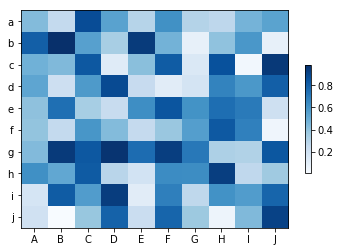
\includegraphics[width=0.95\linewidth,height=0.7\textheight,keepaspectratio]{03_WXN_matplotlib_files/03_WXN_matplotlib_48_0} \end{center}

\begin{Shaded}
\begin{Highlighting}[]
\ImportTok{import} \NormalTok{pandas }\ImportTok{as} \NormalTok{pd}
\ImportTok{import} \NormalTok{numpy }\ImportTok{as} \NormalTok{np}
\NormalTok{df }\OperatorTok{=} \NormalTok{pd.DataFrame(np.random.randn(}\DecValTok{5}\NormalTok{, }\DecValTok{6}\NormalTok{))}
\NormalTok{df}
\end{Highlighting}
\end{Shaded}

\begin{verbatim}
<tr style="text-align: right;">
  <th></th>
  <th>0</th>
  <th>1</th>
  <th>2</th>
  <th>3</th>
  <th>4</th>
  <th>5</th>
</tr>
\end{verbatim}

\begin{verbatim}
<tr>
  <th>0</th>
  <td>-0.596967</td>
  <td>0.080979</td>
  <td>-1.890122</td>
  <td>-0.629949</td>
  <td>-1.187113</td>
  <td>-0.002018</td>
</tr>
<tr>
  <th>1</th>
  <td>1.264042</td>
  <td>0.044216</td>
  <td>-1.669342</td>
  <td>0.805476</td>
  <td>-0.173634</td>
  <td>-0.051918</td>
</tr>
<tr>
  <th>2</th>
  <td>0.793684</td>
  <td>1.746997</td>
  <td>0.785712</td>
  <td>-0.157126</td>
  <td>0.072688</td>
  <td>0.310271</td>
</tr>
<tr>
  <th>3</th>
  <td>0.988716</td>
  <td>0.404472</td>
  <td>0.967111</td>
  <td>-0.612160</td>
  <td>-0.259917</td>
  <td>-0.067299</td>
</tr>
<tr>
  <th>4</th>
  <td>0.033911</td>
  <td>1.177149</td>
  <td>-0.914153</td>
  <td>-0.579912</td>
  <td>-0.100110</td>
  <td>0.747296</td>
</tr>
\end{verbatim}

\begin{Shaded}
\begin{Highlighting}[]
\NormalTok{plt.imshow(df)}

\NormalTok{plt.show()}
\end{Highlighting}
\end{Shaded}

\begin{center}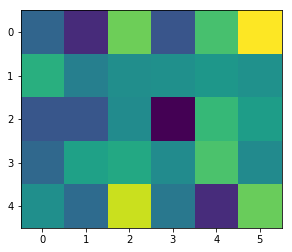
\includegraphics[width=0.95\linewidth,height=0.7\textheight,keepaspectratio]{03_WXN_matplotlib_files/03_WXN_matplotlib_50_0} \end{center}

读入基因表达数据,绘制某基因的箱线图

\begin{Shaded}
\begin{Highlighting}[]
\OperatorTok{%}\NormalTok{cd F: }\OperatorTok{\textbackslash{}}\NormalTok{mega}\OperatorTok{\textbackslash{}}\NormalTok{ehbio}\OperatorTok{\textbackslash{}}\NormalTok{python}\OperatorTok{\textbackslash{}}\NormalTok{python课程包}\OperatorTok{\textbackslash{}}\NormalTok{merge}
\ImportTok{import} \NormalTok{os}
\NormalTok{os.getcwd()}
\end{Highlighting}
\end{Shaded}

\begin{verbatim}
F:\mega\ehbio\python\python课程包\merge





'F:\\mega\\ehbio\\python\\python课程包\\merge'
\end{verbatim}

\begin{Shaded}
\begin{Highlighting}[]
\ImportTok{import} \NormalTok{pandas }\ImportTok{as} \NormalTok{pd}
\NormalTok{df }\OperatorTok{=} \NormalTok{pd.read_table(}\StringTok{"ehbio.xls"}\NormalTok{, sep}\OperatorTok{=}\StringTok{"}\CharTok{\textbackslash{}t}\StringTok{"}\NormalTok{, index_col}\OperatorTok{=}\DecValTok{0}\NormalTok{, header}\OperatorTok{=}\DecValTok{0}\NormalTok{)}
\NormalTok{df.head(}\DecValTok{5}\NormalTok{)}
\end{Highlighting}
\end{Shaded}

\begin{verbatim}
<tr style="text-align: right;">
  <th></th>
  <th>MCF10F</th>
  <th>MCF12A</th>
  <th>T47DKBluc</th>
  <th>UACC812</th>
  <th>UACC893</th>
  <th>ZR751</th>
  <th>ZR7530</th>
  <th>ZR75B</th>
</tr>
<tr>
  <th>EnsEMBL_Gene_ID</th>
  <th></th>
  <th></th>
  <th></th>
  <th></th>
  <th></th>
  <th></th>
  <th></th>
  <th></th>
</tr>
\end{verbatim}

\begin{verbatim}
<tr>
  <th>ENSG00000000003</th>
  <td>91.574061</td>
  <td>13.040870</td>
  <td>73.387310</td>
  <td>26.579280</td>
  <td>50.676579</td>
  <td>31.812999</td>
  <td>121.459918</td>
  <td>2.293898</td>
</tr>
<tr>
  <th>ENSG00000001167</th>
  <td>164.221408</td>
  <td>170.101403</td>
  <td>106.114416</td>
  <td>138.140311</td>
  <td>106.342032</td>
  <td>68.458022</td>
  <td>73.910964</td>
  <td>61.625519</td>
</tr>
<tr>
  <th>ENSG00000005471</th>
  <td>0.000000</td>
  <td>0.073680</td>
  <td>0.536226</td>
  <td>0.440649</td>
  <td>0.066213</td>
  <td>0.548865</td>
  <td>0.611036</td>
  <td>0.556531</td>
</tr>
<tr>
  <th>ENSG00000066629</th>
  <td>24.630773</td>
  <td>18.627459</td>
  <td>34.619613</td>
  <td>79.187879</td>
  <td>0.058835</td>
  <td>25.493800</td>
  <td>25.917323</td>
  <td>32.528112</td>
</tr>
<tr>
  <th>ENSG00000154258</th>
  <td>0.896612</td>
  <td>0.214261</td>
  <td>0.000000</td>
  <td>0.040907</td>
  <td>0.021120</td>
  <td>0.000000</td>
  <td>0.033571</td>
  <td>0.177808</td>
</tr>
\end{verbatim}

\begin{Shaded}
\begin{Highlighting}[]
\NormalTok{df.shape}
\end{Highlighting}
\end{Shaded}

\begin{verbatim}
(36953, 8)
\end{verbatim}

\begin{Shaded}
\begin{Highlighting}[]
\NormalTok{df.size}
\NormalTok{df.ndim}
\NormalTok{df.values}
\end{Highlighting}
\end{Shaded}

\begin{verbatim}
array([[  9.15740610e+01,   1.30408701e+01,   7.33873101e+01, ...,
          3.18129988e+01,   1.21459918e+02,   2.29389818e+00],
       [  1.64221408e+02,   1.70101403e+02,   1.06114416e+02, ...,
          6.84580224e+01,   7.39109636e+01,   6.16255191e+01],
       [  0.00000000e+00,   7.36800986e-02,   5.36226145e-01, ...,
          5.48864965e-01,   6.11036013e-01,   5.56531115e-01],
       ..., 
       [  2.71701826e+00,   5.55925621e+00,   2.93123839e+00, ...,
          3.71765369e+00,   2.42540639e+00,   4.56656068e+00],
       [  1.74266818e+01,   3.72964028e+00,   3.49013629e+01, ...,
          5.04982802e+01,   3.75784692e+01,   4.79996494e+01],
       [  0.00000000e+00,   0.00000000e+00,   3.52988338e+00, ...,
          8.15259649e+00,   6.08178979e-01,   3.25252710e+00]])
\end{verbatim}

\begin{Shaded}
\begin{Highlighting}[]
\NormalTok{control }\OperatorTok{=} \NormalTok{[]}
\ControlFlowTok{for} \NormalTok{i }\OperatorTok{in} \BuiltInTok{range}\NormalTok{(}\DecValTok{3}\NormalTok{):}
    \NormalTok{control.append(df.iloc[}\DecValTok{0}\NormalTok{, i])}
\NormalTok{control}
\end{Highlighting}
\end{Shaded}

\begin{verbatim}
[91.574060981100004, 13.0408701074, 73.387310079800002]
\end{verbatim}

\begin{Shaded}
\begin{Highlighting}[]
\NormalTok{test }\OperatorTok{=} \NormalTok{[]}
\ControlFlowTok{for} \NormalTok{i }\OperatorTok{in} \BuiltInTok{range}\NormalTok{(}\DecValTok{3}\NormalTok{, }\DecValTok{8}\NormalTok{):}
    \NormalTok{test.append(df.iloc[}\DecValTok{0}\NormalTok{, i])}
\NormalTok{test}
\end{Highlighting}
\end{Shaded}

\begin{verbatim}
[26.579280359299997,
 50.676578905299998,
 31.812998762600003,
 121.4599177489,
 2.2938981847999997]
\end{verbatim}

\begin{Shaded}
\begin{Highlighting}[]
\NormalTok{gene }\OperatorTok{=} \NormalTok{[control, test]}
\end{Highlighting}
\end{Shaded}

\begin{Shaded}
\begin{Highlighting}[]
\NormalTok{fig }\OperatorTok{=} \NormalTok{plt.figure()}
\NormalTok{ax }\OperatorTok{=} \NormalTok{fig.add_subplot(}\DecValTok{1}\NormalTok{, }\DecValTok{1}\NormalTok{, }\DecValTok{1}\NormalTok{)}
\NormalTok{ax.boxplot(gene, patch_artist}\OperatorTok{=}\VariableTok{True}\NormalTok{,  }\CommentTok{# 箱体添加颜色}
           \NormalTok{labels}\OperatorTok{=}\NormalTok{[}\StringTok{'test'}\NormalTok{, }\StringTok{'control'}\NormalTok{],  }\CommentTok{# 添加具体的标签名称}
           \NormalTok{showmeans}\OperatorTok{=}\VariableTok{True}\NormalTok{, )}
\NormalTok{plt.show()}
\end{Highlighting}
\end{Shaded}

\begin{center}\includegraphics[width=0.95\linewidth,height=0.7\textheight,keepaspectratio]{03_WXN_matplotlib_files/03_WXN_matplotlib_59_0} \end{center}

热图

\begin{Shaded}
\begin{Highlighting}[]
\NormalTok{df2 }\OperatorTok{=} \NormalTok{df.head(}\DecValTok{10}\NormalTok{)  }\CommentTok{# 取部分数据}
\end{Highlighting}
\end{Shaded}

\begin{Shaded}
\begin{Highlighting}[]
\NormalTok{df2}
\end{Highlighting}
\end{Shaded}

\begin{verbatim}
<tr style="text-align: right;">
  <th></th>
  <th>MCF10F</th>
  <th>MCF12A</th>
  <th>T47DKBluc</th>
  <th>UACC812</th>
  <th>UACC893</th>
  <th>ZR751</th>
  <th>ZR7530</th>
  <th>ZR75B</th>
</tr>
<tr>
  <th>EnsEMBL_Gene_ID</th>
  <th></th>
  <th></th>
  <th></th>
  <th></th>
  <th></th>
  <th></th>
  <th></th>
  <th></th>
</tr>
\end{verbatim}

\begin{verbatim}
<tr>
  <th>ENSG00000000003</th>
  <td>91.574061</td>
  <td>13.040870</td>
  <td>73.387310</td>
  <td>26.579280</td>
  <td>50.676579</td>
  <td>31.812999</td>
  <td>121.459918</td>
  <td>2.293898</td>
</tr>
<tr>
  <th>ENSG00000001167</th>
  <td>164.221408</td>
  <td>170.101403</td>
  <td>106.114416</td>
  <td>138.140311</td>
  <td>106.342032</td>
  <td>68.458022</td>
  <td>73.910964</td>
  <td>61.625519</td>
</tr>
<tr>
  <th>ENSG00000005471</th>
  <td>0.000000</td>
  <td>0.073680</td>
  <td>0.536226</td>
  <td>0.440649</td>
  <td>0.066213</td>
  <td>0.548865</td>
  <td>0.611036</td>
  <td>0.556531</td>
</tr>
<tr>
  <th>ENSG00000066629</th>
  <td>24.630773</td>
  <td>18.627459</td>
  <td>34.619613</td>
  <td>79.187879</td>
  <td>0.058835</td>
  <td>25.493800</td>
  <td>25.917323</td>
  <td>32.528112</td>
</tr>
<tr>
  <th>ENSG00000154258</th>
  <td>0.896612</td>
  <td>0.214261</td>
  <td>0.000000</td>
  <td>0.040907</td>
  <td>0.021120</td>
  <td>0.000000</td>
  <td>0.033571</td>
  <td>0.177808</td>
</tr>
<tr>
  <th>ENSG00000154262</th>
  <td>3.431313</td>
  <td>2.481636</td>
  <td>0.000000</td>
  <td>0.383060</td>
  <td>0.000000</td>
  <td>0.000000</td>
  <td>0.000000</td>
  <td>0.105758</td>
</tr>
<tr>
  <th>ENSG00000154263</th>
  <td>0.859071</td>
  <td>0.936069</td>
  <td>0.589547</td>
  <td>0.259898</td>
  <td>0.083258</td>
  <td>0.476794</td>
  <td>0.526162</td>
  <td>0.221172</td>
</tr>
<tr>
  <th>ENSG00000154265</th>
  <td>2.453971</td>
  <td>1.480553</td>
  <td>9.884425</td>
  <td>2.076723</td>
  <td>1.118819</td>
  <td>5.864268</td>
  <td>10.180796</td>
  <td>4.383174</td>
</tr>
<tr>
  <th>ENSG00000154269</th>
  <td>0.216739</td>
  <td>0.000000</td>
  <td>0.854111</td>
  <td>0.970053</td>
  <td>0.738803</td>
  <td>0.521094</td>
  <td>4.648410</td>
  <td>0.000000</td>
</tr>
<tr>
  <th>ENSG00000154274</th>
  <td>2.980792</td>
  <td>0.217999</td>
  <td>276.123679</td>
  <td>82.820443</td>
  <td>34.664053</td>
  <td>106.350607</td>
  <td>94.854069</td>
  <td>14.976808</td>
</tr>
\end{verbatim}

\begin{Shaded}
\begin{Highlighting}[]
\NormalTok{i }\OperatorTok{=} \NormalTok{plt.imshow(df2)}
\NormalTok{plt.colorbar(i)}
\NormalTok{plt.show()}
\end{Highlighting}
\end{Shaded}

\begin{center}\includegraphics[width=0.95\linewidth,height=0.7\textheight,keepaspectratio]{03_WXN_matplotlib_files/03_WXN_matplotlib_63_0} \end{center}

\url{https://matplotlib.org/api/pyplot_api.html\#所有函数的详细参数}。

\section{Python实战}\label{Py3ux5fpratciseux5fct}

欢迎访问我们的视频课程 \url{https://bioinfo.ke.qq.com}。

\subsection{Python实战}\label{python}

\subsubsection{ID转换}\label{id}

不同数据库的名字互相转换,比如NCBI的ENTEZ ID转Gene
symbol,ENSEMBL编号转ENTREZ ID。

ID转换一般需要2个文件,一个文件是要转换的ID,另外一个文件是ID的对应关系。

以我们的测试文件
(\textbf{GRCh38.idmap})为例,第一列为\texttt{ENSEMBLE\ ID},第二列为\texttt{Gene\ symbol},第三列为\texttt{Entrez\ ID}。

\begin{verbatim}
Gene ID Associated Gene Name    EntrezGene ID
ENSG00000252303 RNU6-280P       
ENSG00000281771 Y_RNA      
ENSG00000281876 RP11-399E6.4    101929901
ENSG00000281766 RYBP    23429
ENSG00000281518 FOXO6   100132074
ENSG00000281614 INPP5D  3635
ENSG00000280584 OBP2B   29989
ENSG00000281230 SERTAD4 56256
ENSG00000281917 SLC16A1 6566
\end{verbatim}

待转换的文件 (\textbf{ensm.id})内容为,期望转换为\texttt{Gene\ symbol}。

\begin{verbatim}
ENSG00000252303
ENSG00000281771
ENSG00000281256
ENSG00000283272
ENSG00000280864
ENSG00000280792
ENSG00000282878
ENSG00000283276
ENSG00000281822
ENSG00000281384
ENSG00000280505
ENSG00000281764
ENSG00000281316
ENSG00000280963
ENSG00000280775
ENSG00000281876
ENSG00000281766
ENSG00000281518
ENSG00000281614
ENSG00000280584
ENSG00000281230
ENSG00000281917
\end{verbatim}

我们怎么做呢?
直观看起来也比较简单,一个个的去比较、匹配、提取就可以了。

\begin{Shaded}
\begin{Highlighting}[]
\NormalTok{idD }\OperatorTok{=} \NormalTok{\{\}}
\ControlFlowTok{for} \NormalTok{line }\OperatorTok{in} \BuiltInTok{open}\NormalTok{(}\StringTok{"data/GRCh38.idmap"}\NormalTok{):}
    \NormalTok{lineL }\OperatorTok{=} \NormalTok{line.strip().split(}\StringTok{"}\CharTok{\textbackslash{}t}\StringTok{"}\NormalTok{)}
    \NormalTok{ensm_id }\OperatorTok{=} \NormalTok{lineL[}\DecValTok{0}\NormalTok{]}
    \NormalTok{symbol  }\OperatorTok{=} \NormalTok{lineL[}\DecValTok{1}\NormalTok{]}
    \NormalTok{idD[ensm_id] }\OperatorTok{=} \NormalTok{symbol}
\CommentTok{#--------------------------------}
\ControlFlowTok{for} \NormalTok{line }\OperatorTok{in} \BuiltInTok{open}\NormalTok{(}\StringTok{"data/ensm.id"}\NormalTok{):}
    \NormalTok{ensm }\OperatorTok{=} \NormalTok{line.strip()}
    \BuiltInTok{print}\NormalTok{(ensm,idD[ensm],sep}\OperatorTok{=}\StringTok{": "}\NormalTok{)}
\end{Highlighting}
\end{Shaded}

\begin{verbatim}
ENSG00000252303: RNU6-280P
ENSG00000281771: Y_RNA
ENSG00000281256: RP11-222G7.2
ENSG00000283272: Clostridiales-1
ENSG00000280864: RP11-654C22.2
ENSG00000280792: RP11-315F22.1
ENSG00000282878: RP11-399E6.1
ENSG00000283276: ABBA01000934.1
ENSG00000281822: RNU1-62P
ENSG00000281384: AC093802.1
ENSG00000280505: RP11-654C22.1
ENSG00000281764: RP11-399E6.2
ENSG00000281316: DPPA2P2
ENSG00000280963: SERTAD4-AS1
ENSG00000280775: RNA5SP136
ENSG00000281876: RP11-399E6.4
ENSG00000281766: RYBP
ENSG00000281518: FOXO6
ENSG00000281614: INPP5D
ENSG00000280584: OBP2B
ENSG00000281230: SERTAD4
ENSG00000281917: SLC16A1
\end{verbatim}

\begin{Shaded}
\begin{Highlighting}[]
\CommentTok{# 首先读入GRCh38.idmap文件}

\CommentTok{# 定义3个变量,文件名,ensembl_id所在列(0-start, source_col), symbol所在列 (1,target_col)}
\CommentTok{# 提前定义的好处是,修改起来会比较方便。}
\NormalTok{map_file }\OperatorTok{=} \StringTok{"data/GRCh38.idmap"}
\NormalTok{source_col }\OperatorTok{=} \DecValTok{0}
\NormalTok{target_col }\OperatorTok{=} \DecValTok{1}
\NormalTok{aDict }\OperatorTok{=} \NormalTok{\{\}}
\ControlFlowTok{for} \NormalTok{line }\OperatorTok{in} \BuiltInTok{open}\NormalTok{(map_file):}
    \NormalTok{lineL }\OperatorTok{=} \NormalTok{line.strip().split(}\StringTok{"}\CharTok{\textbackslash{}t}\StringTok{"}\NormalTok{)}
    \NormalTok{source }\OperatorTok{=} \NormalTok{lineL[source_col]}
    \NormalTok{target }\OperatorTok{=} \NormalTok{lineL[target_col]}
    \NormalTok{aDict[source] }\OperatorTok{=} \NormalTok{target}

\CommentTok{# 读入ensm.id文件}
\CommentTok{# 边读边处理}

\NormalTok{id_file }\OperatorTok{=} \StringTok{"data/ensm.id"}
\ControlFlowTok{for} \NormalTok{line }\OperatorTok{in} \BuiltInTok{open}\NormalTok{(id_file):}
    \NormalTok{source_id }\OperatorTok{=} \NormalTok{line.strip()}
    \NormalTok{map_id }\OperatorTok{=} \NormalTok{aDict.get(source_id, source_id)}
    \BuiltInTok{print}\NormalTok{(map_id)}

\CommentTok{# 输出到文件}

\ControlFlowTok{with} \BuiltInTok{open}\NormalTok{(}\StringTok{"data/symbol.id"}\NormalTok{,}\StringTok{"w"}\NormalTok{) }\ImportTok{as} \NormalTok{fh:}
    \NormalTok{id_file }\OperatorTok{=} \StringTok{"data/ensm.id"}
    \ControlFlowTok{for} \NormalTok{line }\OperatorTok{in} \BuiltInTok{open}\NormalTok{(id_file):}
        \NormalTok{source_id }\OperatorTok{=} \NormalTok{line.strip()}
        \NormalTok{map_id }\OperatorTok{=} \NormalTok{aDict.get(source_id, source_id)}
        \BuiltInTok{print}\NormalTok{(map_id, }\BuiltInTok{file}\OperatorTok{=}\NormalTok{fh)}
\end{Highlighting}
\end{Shaded}

\begin{verbatim}
RNU6-280P
Y_RNA
RP11-222G7.2
Clostridiales-1
RP11-654C22.2
RP11-315F22.1
RP11-399E6.1
ABBA01000934.1
RNU1-62P
AC093802.1
RP11-654C22.1
RP11-399E6.2
DPPA2P2
SERTAD4-AS1
RNA5SP136
RP11-399E6.4
RYBP
FOXO6
INPP5D
OBP2B
SERTAD4
SLC16A1
\end{verbatim}

\subsubsection{每条染色体基因数目统计}

GTF文件存储基因的注释信息。

\begin{enumerate}
\def\labelenumi{\arabic{enumi}.}
\tightlist
\item
  seqname - name of the chromosome or scaffold; chromosome names can be
  given with or without the `chr' prefix. Important note: the seqname
  must be one used within Ensembl, i.e.~a standard chromosome name or an
  Ensembl identifier such as a scaffold ID, without any additional
  content such as species or assembly. See the example GFF output below.
\item
  source - name of the program that generated this feature, or the data
  source (database or project name)
\item
  feature - feature type name, e.g.~Gene, Variation, Similarity
\item
  start - Start position of the feature, with sequence numbering
  starting at 1.
\item
  end - End position of the feature, with sequence numbering starting at
  1.
\item
  score - A floating point value.
\item
  strand - defined as + (forward) or - (reverse).
\item
  frame - One of `0', `1' or `2'. `0' indicates that the first base of
  the feature is the first base of a codon, `1' that the second base is
  the first base of a codon, and so on..
\item
  attribute - A semicolon-separated list of tag-value pairs, providing
  additional information about each feature.
\end{enumerate}

\begin{verbatim}
chr1    HAVANA  gene    11869   14409   .   +   .   gene_id "ENSG00000223972.5"; gene_type "transcribed_unprocessed_pseudogene"; gene_status "KNOWN"; gene_name "DDX11L1";  level 2; havana_gene "OTTHUMG00000000961.2";
chr1    HAVANA  gene    14404   29570   .   -   .   gene_id "ENSG00000227232.5"; gene_type "unprocessed_pseudogene"; gene_status "KNOWN"; gene_name "WASH7P";  level 2; havana_gene "OTTHUMG00000000958.1";
chr1    ENSEMBL gene    17369   17436   .   -   .   gene_id "ENSG00000278267.1"; gene_type "miRNA"; gene_status "KNOWN"; gene_name "MIR6859-3";  level 3;
\end{verbatim}

如果统计每条染色体基因数目,只需要读第一列和第三列就可以了。

\begin{Shaded}
\begin{Highlighting}[]
\NormalTok{chr_gene_cntD }\OperatorTok{=} \NormalTok{\{\}}
\ControlFlowTok{for} \NormalTok{line }\OperatorTok{in} \BuiltInTok{open}\NormalTok{(}\StringTok{"data/gencode.gene.gtf"}\NormalTok{):}
    \NormalTok{lineL }\OperatorTok{=} \NormalTok{line.strip().split(}\StringTok{"}\CharTok{\textbackslash{}t}\StringTok{"}\NormalTok{)}
    \NormalTok{chrName }\OperatorTok{=} \NormalTok{lineL[}\DecValTok{0}\NormalTok{]}
    \NormalTok{regionType }\OperatorTok{=} \NormalTok{lineL[}\DecValTok{2}\NormalTok{]}
    \ControlFlowTok{if} \NormalTok{(regionType }\OperatorTok{==} \StringTok{"gene"}\NormalTok{):}
        \ControlFlowTok{if} \NormalTok{chrName }\OperatorTok{not} \OperatorTok{in} \NormalTok{chr_gene_cntD:}
            \NormalTok{chr_gene_cntD[chrName] }\OperatorTok{=} \DecValTok{1}
        \ControlFlowTok{else}\NormalTok{:}
            \NormalTok{chr_gene_cntD[chrName] }\OperatorTok{+=} \DecValTok{1}
\CommentTok{#---------------------------------}
\ControlFlowTok{for} \NormalTok{chrName, cnt }\OperatorTok{in} \BuiltInTok{list}\NormalTok{(chr_gene_cntD.items()):}
    \BuiltInTok{print}\NormalTok{(chrName,}\StringTok{"has"}\NormalTok{,cnt,}\StringTok{'genes.'}\NormalTok{)}
\end{Highlighting}
\end{Shaded}

\begin{verbatim}
chr1 has 5397 genes.
chr2 has 4150 genes.
chr3 has 3163 genes.
chr4 has 2633 genes.
chr5 has 2993 genes.
chr6 has 3001 genes.
chr7 has 2980 genes.
chr8 has 2444 genes.
chr9 has 2350 genes.
chr10 has 2306 genes.
chr11 has 3381 genes.
chr12 has 3047 genes.
chr13 has 1383 genes.
chr14 has 2289 genes.
chr15 has 2247 genes.
chr16 has 2597 genes.
chr17 has 3111 genes.
chr18 has 1206 genes.
chr19 has 2997 genes.
chr20 has 1436 genes.
chr21 has 880 genes.
chr22 has 1385 genes.
chrX has 2476 genes.
chrY has 594 genes.
chrM has 37 genes.
\end{verbatim}

\begin{Shaded}
\begin{Highlighting}[]
\NormalTok{gtf_file }\OperatorTok{=} \StringTok{"data/gencode.gene.gtf"}

\CommentTok{# 一般字典命名,会在行尾加一个大写的D,作为类型代表}
\NormalTok{chr_gene_cntD }\OperatorTok{=} \NormalTok{\{\}}

\ControlFlowTok{for} \NormalTok{line }\OperatorTok{in} \BuiltInTok{open}\NormalTok{(gtf_file):}
    \CommentTok{# 每行按TAB键分成4份}
    \NormalTok{lineL }\OperatorTok{=} \NormalTok{line.split(}\StringTok{'}\CharTok{\textbackslash{}t}\StringTok{'}\NormalTok{,}\DecValTok{3}\NormalTok{)}
    \NormalTok{chr_name }\OperatorTok{=} \NormalTok{lineL[}\DecValTok{0}\NormalTok{]}
    \NormalTok{feature  }\OperatorTok{=} \NormalTok{lineL[}\DecValTok{2}\NormalTok{]}
    \ControlFlowTok{if} \NormalTok{feature }\OperatorTok{==} \StringTok{"gene"}\NormalTok{:}
        \CommentTok{# 如果chr_name已经出现过,则获取其值,然后加1}
        \CommentTok{# 若没出现过,获取0,加1,表示第一次出现}
        \NormalTok{chr_gene_cntD[chr_name] }\OperatorTok{=} \NormalTok{chr_gene_cntD.get(chr_name,}\DecValTok{0}\NormalTok{) }\OperatorTok{+} \DecValTok{1}
\CommentTok{#--------------------------------------}
\ControlFlowTok{for} \NormalTok{chr_name, count }\OperatorTok{in} \NormalTok{chr_gene_cntD.items():}
    \BuiltInTok{print}\NormalTok{(chr_name, count)}
\end{Highlighting}
\end{Shaded}

\begin{verbatim}
chr1 5397
chr2 4150
chr3 3163
chr4 2633
chr5 2993
chr6 3001
chr7 2980
chr8 2444
chr9 2350
chr10 2306
chr11 3381
chr12 3047
chr13 1383
chr14 2289
chr15 2247
chr16 2597
chr17 3111
chr18 1206
chr19 2997
chr20 1436
chr21 880
chr22 1385
chrX 2476
chrY 594
chrM 37
\end{verbatim}

\subsubsection{所有外显子总长度统计}

bed12格式 (前3列必须,其它可选)

\begin{enumerate}
\def\labelenumi{\arabic{enumi}.}
\item
  chrom - The name of the chromosome (e.g.~chr3, chrY, chr2\_random) or
  scaffold (e.g.~scaffold10671).
\item
  chromStart - The starting position of the feature in the chromosome or
  scaffold. The first base in a chromosome is numbered 0.
\item
  chromEnd - The ending position of the feature in the chromosome or
  scaffold. The chromEnd base is not included in the display of the
  feature.
\item
  name - Defines the name of the BED line. This label is displayed to
  the left of the BED line in the Genome Browser window when the track
  is open to full display mode or directly to the left of the item in
  pack mode.
\item
  score - A score between 0 and 1000. If the track line useScore
  attribute is set to 1 for this annotation data set, the score value
  will determine the level of gray in which this feature is displayed
  (higher numbers = darker gray). This table shows the Genome Browser's
  translation of BED score values into shades of gray:
\item
  thickStart - The starting position at which the feature is drawn
  thickly (for example, the start codon in gene displays). When there is
  no thick part, thickStart and thickEnd are usually set to the
  chromStart position.
\item
  thickEnd - The ending position at which the feature is drawn thickly
  (for example the stop codon in gene displays).
\item
  itemRgb - An RGB value of the form R,G,B (e.g.~255,0,0). If the track
  line itemRgb attribute is set to ``On'', this RBG value will determine
  the display color of the data contained in this BED line. NOTE: It is
  recommended that a simple color scheme (eight colors or less) be used
  with this attribute to avoid overwhelming the color resources of the
  Genome Browser and your Internet browser.
\item
  blockCount - The number of blocks (exons) in the BED line.
\item
  blockSizes - A comma-separated list of the block sizes. The number of
  items in this list should correspond to blockCount.
\item
  blockStarts - A comma-separated list of block starts. All of the
  blockStart positions should be calculated relative to chromStart. The
  number of items in this list should correspond to blockCount.
\end{enumerate}

基因注释bed12格式

\begin{verbatim}
chr1    11868   14409   ENST00000456328.2   0   +   14409   14409   0   3   359,109,1189,   0,744,1352,
chr1    12009   13670   ENST00000450305.2   0   +   13670   13670   0   6   48,49,85,78,154,218,    0,169,603,965,1211,1443,
chr1    17368   17436   ENST00000619216.1   0   -   17436   17436   0   1   68, 0,
chr1    29553   31097   ENST00000473358.1   0   +   31097   31097   0   3   486,104,122,    0,1010,1422,
chr1    30266   31109   ENST00000469289.1   0   +   31109   31109   0   2   401,134,    0,709,
chr1    30365   30503   ENST00000607096.1   0   +   30503   30503   0   1   138,    0,
\end{verbatim}

第十列是外显子的大小,所有我们只需要把他们加在一起就好了。

\textbf{Note}:实际计算时需要考虑不同转录本之间存在重叠,需要对bed文件预处理,只保留唯一的外显子位置,然后再加和。

\begin{Shaded}
\begin{Highlighting}[]
\NormalTok{exonSizeSum }\OperatorTok{=} \DecValTok{0}
\ControlFlowTok{for} \NormalTok{line }\OperatorTok{in} \BuiltInTok{open}\NormalTok{(}\StringTok{"data/gencode.gene.bed12"}\NormalTok{):}
    \NormalTok{lineL }\OperatorTok{=} \NormalTok{line.split()}
    \NormalTok{exonSize }\OperatorTok{=} \NormalTok{lineL[}\DecValTok{10}\NormalTok{]}
    \NormalTok{exonSizeL }\OperatorTok{=} \NormalTok{exonSize.strip(}\StringTok{','}\NormalTok{).split(}\StringTok{','}\NormalTok{)}
    \ControlFlowTok{for} \NormalTok{i }\OperatorTok{in} \NormalTok{exonSizeL:}
        \NormalTok{exonSizeSum }\OperatorTok{+=} \BuiltInTok{int}\NormalTok{(i)}
\BuiltInTok{print}\NormalTok{(exonSizeSum)}
\end{Highlighting}
\end{Shaded}

\begin{verbatim}
291762517
\end{verbatim}

\begin{Shaded}
\begin{Highlighting}[]
\NormalTok{bed12 }\OperatorTok{=} \StringTok{"data/gencode.gene.bed12"}

\NormalTok{total_exon_sum }\OperatorTok{=} \DecValTok{0}

\ControlFlowTok{for} \NormalTok{line }\OperatorTok{in} \BuiltInTok{open}\NormalTok{(bed12):}
    \CommentTok{# 从右侧分割为3个元素的列表}
    \CommentTok{# 关注的元素在第二位,索引为1}
    \CommentTok{# 去掉末尾的逗号}
    \NormalTok{lineL }\OperatorTok{=} \NormalTok{line.rsplit(}\StringTok{"}\CharTok{\textbackslash{}t}\StringTok{"}\NormalTok{,}\DecValTok{2}\NormalTok{)}
    \NormalTok{exonSize }\OperatorTok{=} \NormalTok{lineL[}\DecValTok{1}\NormalTok{].strip(}\StringTok{','}\NormalTok{)}
    \NormalTok{exonSizeL }\OperatorTok{=} \NormalTok{[}\BuiltInTok{int}\NormalTok{(i) }\ControlFlowTok{for} \NormalTok{i }\OperatorTok{in} \NormalTok{exonSize.split(}\StringTok{','}\NormalTok{)]}
    \NormalTok{exonSum }\OperatorTok{=} \BuiltInTok{sum}\NormalTok{(exonSizeL)}
    
    \NormalTok{total_exon_sum }\OperatorTok{+=} \NormalTok{exonSum}
\BuiltInTok{print}\NormalTok{(}\StringTok{"Total exon size is"}\NormalTok{, total_exon_sum, }\StringTok{"nt."}\NormalTok{)}

\CommentTok{# 更清晰展示数字大小}
\BuiltInTok{print}\NormalTok{(}\StringTok{"Total exon size is"}\NormalTok{, }\StringTok{"\{:,\}"}\NormalTok{.}\BuiltInTok{format}\NormalTok{(total_exon_sum), }\StringTok{"nt."}\NormalTok{)}
\end{Highlighting}
\end{Shaded}

\begin{verbatim}
Total exon size is 291762517 nt.
Total exon size is 291,762,517 nt.
\end{verbatim}

\begin{Shaded}
\begin{Highlighting}[]
\BuiltInTok{print}\NormalTok{(}\StringTok{"}\SpecialCharTok{\{a[a]\}}\StringTok{"}\NormalTok{.}\BuiltInTok{format}\NormalTok{(a}\OperatorTok{=}\NormalTok{\{}\StringTok{'a'}\NormalTok{:}\StringTok{"ehbio"}\NormalTok{\}))}
\end{Highlighting}
\end{Shaded}

\begin{verbatim}
ehbio
\end{verbatim}

\subsection{Python小技巧}\label{python}

链似比较

\begin{Shaded}
\begin{Highlighting}[]
\NormalTok{x }\OperatorTok{=} \DecValTok{5}
\BuiltInTok{print}\NormalTok{(}\StringTok{"1 < x < 10 is"}\NormalTok{, }\DecValTok{1} \OperatorTok{<} \NormalTok{x }\OperatorTok{<} \DecValTok{10}\NormalTok{)}
\BuiltInTok{print}\NormalTok{(}\StringTok{"10 > x <= 9"}\NormalTok{, }\DecValTok{10} \OperatorTok{>} \NormalTok{x }\OperatorTok{<=} \DecValTok{9}\NormalTok{)}
\end{Highlighting}
\end{Shaded}

\begin{verbatim}
1 < x < 10 is True
10 > x <= 9 True
\end{verbatim}

解释正则表达式

\begin{Shaded}
\begin{Highlighting}[]
\ImportTok{import} \NormalTok{re}
\NormalTok{re.}\BuiltInTok{compile}\NormalTok{(}\StringTok{"^[a-z]*$"}\NormalTok{, re.DEBUG)}
\end{Highlighting}
\end{Shaded}

\begin{verbatim}
AT AT_BEGINNING
MAX_REPEAT 0 MAXREPEAT
  IN
    RANGE (97, 122)
AT AT_END





re.compile(r'^[a-z]*$', re.UNICODE|re.DEBUG)
\end{verbatim}

\begin{Shaded}
\begin{Highlighting}[]
\NormalTok{re.}\BuiltInTok{compile}\NormalTok{(}\StringTok{"^[a-z][0-9]+$"}\NormalTok{, re.DEBUG)}
\end{Highlighting}
\end{Shaded}

\begin{verbatim}
AT AT_BEGINNING
IN
  RANGE (97, 122)
MAX_REPEAT 1 MAXREPEAT
  IN
    RANGE (48, 57)
AT AT_END





re.compile(r'^[a-z][0-9]+$', re.UNICODE|re.DEBUG)
\end{verbatim}

\begin{Shaded}
\begin{Highlighting}[]
\NormalTok{re.}\BuiltInTok{compile}\NormalTok{(}\StringTok{"^[a-z]([0-9]+)$"}\NormalTok{, re.DEBUG)}
\end{Highlighting}
\end{Shaded}

\begin{verbatim}
AT AT_BEGINNING
IN
  RANGE (97, 122)
SUBPATTERN 1 0 0
  MAX_REPEAT 1 MAXREPEAT
    IN
      RANGE (48, 57)
AT AT_END





re.compile(r'^[a-z]([0-9]+)$', re.UNICODE|re.DEBUG)
\end{verbatim}

enumerate (不再使用len)

\begin{Shaded}
\begin{Highlighting}[]
\NormalTok{a }\OperatorTok{=} \NormalTok{[}\StringTok{'s'}\NormalTok{,}\StringTok{'x'}\NormalTok{,}\StringTok{'b'}\NormalTok{,}\StringTok{'d'}\NormalTok{]}

\CommentTok{# Preferred way}
\ControlFlowTok{for} \NormalTok{index, item }\OperatorTok{in} \BuiltInTok{enumerate}\NormalTok{(a):}
    \BuiltInTok{print}\NormalTok{(index,item)}

\BuiltInTok{print}\NormalTok{(}\StringTok{"}\CharTok{\textbackslash{}n}\StringTok{"}\NormalTok{)}

\CommentTok{# Old way}
\ControlFlowTok{for} \NormalTok{i }\OperatorTok{in} \BuiltInTok{range}\NormalTok{(}\BuiltInTok{len}\NormalTok{(a)):}
    \BuiltInTok{print}\NormalTok{(i,a[i])}
    
\end{Highlighting}
\end{Shaded}

\begin{verbatim}
0 s
1 x
2 b
3 d


0 s
1 x
2 b
3 d
\end{verbatim}

列表解析、字典解析、元组解析

\begin{Shaded}
\begin{Highlighting}[]
\CommentTok{# 获得系列坐标点}
\NormalTok{a }\OperatorTok{=} \NormalTok{((i,j) }\ControlFlowTok{for} \NormalTok{i }\OperatorTok{in} \BuiltInTok{range}\NormalTok{(}\DecValTok{3}\NormalTok{) }\ControlFlowTok{for} \NormalTok{j }\OperatorTok{in} \BuiltInTok{range}\NormalTok{(}\DecValTok{2}\NormalTok{))}
\NormalTok{a}
\end{Highlighting}
\end{Shaded}

\begin{verbatim}
<generator object <genexpr> at 0x7fa8d04d7fc0>
\end{verbatim}

\begin{Shaded}
\begin{Highlighting}[]
\ControlFlowTok{for} \NormalTok{i }\OperatorTok{in} \NormalTok{a:}
    \BuiltInTok{print}\NormalTok{(i)}
\end{Highlighting}
\end{Shaded}

\begin{verbatim}
(0, 0)
(0, 1)
(1, 0)
(1, 1)
(2, 0)
(2, 1)
\end{verbatim}

\begin{Shaded}
\begin{Highlighting}[]
\NormalTok{str1 }\OperatorTok{=} \StringTok{"I love sheng xin bao dian"}
\BuiltInTok{print}\NormalTok{([i }\ControlFlowTok{for} \NormalTok{i }\OperatorTok{in} \NormalTok{str1.split() }\ControlFlowTok{if} \NormalTok{i.endswith(}\StringTok{'n'}\NormalTok{)])}
\end{Highlighting}
\end{Shaded}

\begin{verbatim}
['xin', 'dian']
\end{verbatim}

\begin{Shaded}
\begin{Highlighting}[]
\NormalTok{a }\OperatorTok{=} \NormalTok{\{i:i}\OperatorTok{*}\DecValTok{2} \ControlFlowTok{for} \NormalTok{i }\OperatorTok{in} \BuiltInTok{range}\NormalTok{(}\DecValTok{5}\NormalTok{)\}}
\NormalTok{a}
\end{Highlighting}
\end{Shaded}

\begin{verbatim}
{0: 0, 1: 2, 2: 4, 3: 6, 4: 8}
\end{verbatim}

\begin{Shaded}
\begin{Highlighting}[]
\NormalTok{[(x, y) }\ControlFlowTok{for} \NormalTok{x }\OperatorTok{in} \BuiltInTok{range}\NormalTok{(}\DecValTok{4}\NormalTok{) }\ControlFlowTok{if} \NormalTok{x }\OperatorTok{%} \DecValTok{2} \OperatorTok{==} \DecValTok{1} \ControlFlowTok{for} \NormalTok{y }\OperatorTok{in} \BuiltInTok{range}\NormalTok{(}\DecValTok{4}\NormalTok{)]}
\end{Highlighting}
\end{Shaded}

\begin{verbatim}
[(1, 0), (1, 1), (1, 2), (1, 3), (3, 0), (3, 1), (3, 2), (3, 3)]
\end{verbatim}

列表索引,反序

\begin{Shaded}
\begin{Highlighting}[]
\NormalTok{a }\OperatorTok{=} \NormalTok{[}\DecValTok{1}\NormalTok{,}\DecValTok{2}\NormalTok{,}\DecValTok{3}\NormalTok{,}\DecValTok{4}\NormalTok{,}\DecValTok{5}\NormalTok{]}
\NormalTok{a[::}\DecValTok{2}\NormalTok{]}
\end{Highlighting}
\end{Shaded}

\begin{verbatim}
[1, 3, 5]
\end{verbatim}

\begin{Shaded}
\begin{Highlighting}[]
\NormalTok{a[::}\OperatorTok{-}\DecValTok{1}\NormalTok{]}
\end{Highlighting}
\end{Shaded}

\begin{verbatim}
[5, 4, 3, 2, 1]
\end{verbatim}

for..else;若\texttt{for}循环中未执行\texttt{break},则\texttt{else}会被执行

\begin{Shaded}
\begin{Highlighting}[]
\NormalTok{found }\OperatorTok{=} \VariableTok{False}
\ControlFlowTok{for} \NormalTok{i }\OperatorTok{in} \BuiltInTok{range}\NormalTok{(}\DecValTok{2}\NormalTok{,}\DecValTok{5}\NormalTok{):}
    \ControlFlowTok{if} \NormalTok{i }\OperatorTok{==} \DecValTok{1}\NormalTok{:}
        \NormalTok{found }\OperatorTok{=} \VariableTok{True}
        \ControlFlowTok{break}
\ControlFlowTok{if} \OperatorTok{not} \NormalTok{found: }
    \BuiltInTok{print}\NormalTok{(}\StringTok{"i was never 1"}\NormalTok{)}
\end{Highlighting}
\end{Shaded}

\begin{verbatim}
i was never 1
\end{verbatim}

\begin{Shaded}
\begin{Highlighting}[]
\ControlFlowTok{for} \NormalTok{i }\OperatorTok{in} \BuiltInTok{range}\NormalTok{(}\DecValTok{2}\NormalTok{,}\DecValTok{5}\NormalTok{):}
    \ControlFlowTok{if} \NormalTok{i }\OperatorTok{==} \DecValTok{1}\NormalTok{:}
        \ControlFlowTok{break}
\ControlFlowTok{else}\NormalTok{:}
    \BuiltInTok{print}\NormalTok{(}\StringTok{"i was never 1"}\NormalTok{)}
\end{Highlighting}
\end{Shaded}

\begin{verbatim}
i was never 1
\end{verbatim}

原位替换

\begin{Shaded}
\begin{Highlighting}[]
\NormalTok{a }\OperatorTok{=} \DecValTok{5}
\NormalTok{b }\OperatorTok{=} \DecValTok{6}
\NormalTok{c }\OperatorTok{=} \DecValTok{7}
\NormalTok{a, b }\OperatorTok{=} \NormalTok{b,a}
\BuiltInTok{print}\NormalTok{(}\StringTok{"a is"}\NormalTok{,a)}
\BuiltInTok{print}\NormalTok{(}\StringTok{"b is"}\NormalTok{,b)}
\end{Highlighting}
\end{Shaded}

\begin{verbatim}
a is 6
b is 5
\end{verbatim}

\begin{Shaded}
\begin{Highlighting}[]
\NormalTok{a, (b,c) }\OperatorTok{=} \NormalTok{c, (a,b)}
\BuiltInTok{print}\NormalTok{(}\StringTok{"a is"}\NormalTok{,a)}
\BuiltInTok{print}\NormalTok{(}\StringTok{"b is"}\NormalTok{,b)}
\BuiltInTok{print}\NormalTok{(}\StringTok{"c is"}\NormalTok{,c)}
\end{Highlighting}
\end{Shaded}

\begin{verbatim}
a is 7
b is 6
c is 5
\end{verbatim}

\begin{Shaded}
\begin{Highlighting}[]
\NormalTok{first, }\OperatorTok{*}\NormalTok{middle_all, last }\OperatorTok{=} \NormalTok{(}\DecValTok{1}\NormalTok{,}\DecValTok{2}\NormalTok{,}\DecValTok{3}\NormalTok{,}\DecValTok{4}\NormalTok{,}\DecValTok{5}\NormalTok{,}\DecValTok{6}\NormalTok{)}
\NormalTok{middle_all}
\end{Highlighting}
\end{Shaded}

\begin{verbatim}
[2, 3, 4, 5]
\end{verbatim}

集合操作

\begin{Shaded}
\begin{Highlighting}[]
\NormalTok{a }\OperatorTok{=} \BuiltInTok{set}\NormalTok{([}\StringTok{"sheng"}\NormalTok{, }\StringTok{"xin"}\NormalTok{, }\StringTok{"bao"}\NormalTok{,}\StringTok{"dian"}\NormalTok{,}\StringTok{"best"}\NormalTok{,}\StringTok{"tutotials"}\NormalTok{])}
\NormalTok{b }\OperatorTok{=} \BuiltInTok{set}\NormalTok{([}\StringTok{"hong"}\NormalTok{, }\StringTok{"ji"}\NormalTok{, }\StringTok{"yin"}\NormalTok{,}\StringTok{"zu"}\NormalTok{,}\StringTok{"best"}\NormalTok{,}\StringTok{"tutotials"}\NormalTok{])}
\NormalTok{a }\OperatorTok{|} \NormalTok{b  }\CommentTok{# union}
\end{Highlighting}
\end{Shaded}

\begin{verbatim}
{'bao', 'best', 'dian', 'hong', 'ji', 'sheng', 'tutotials', 'xin', 'yin', 'zu'}
\end{verbatim}

\begin{Shaded}
\begin{Highlighting}[]
\NormalTok{a }\OperatorTok{&} \NormalTok{b }\CommentTok{# intersection}
\end{Highlighting}
\end{Shaded}

\begin{verbatim}
{'best', 'tutotials'}
\end{verbatim}

\begin{Shaded}
\begin{Highlighting}[]
\NormalTok{a }\OperatorTok{^} \NormalTok{b }\CommentTok{# Symmetric Difference}
\end{Highlighting}
\end{Shaded}

\begin{verbatim}
{'bao', 'dian', 'hong', 'ji', 'sheng', 'xin', 'yin', 'zu'}
\end{verbatim}

Negative round

\begin{Shaded}
\begin{Highlighting}[]
\BuiltInTok{print}\NormalTok{(}\StringTok{"round整数:"}\NormalTok{,}\BuiltInTok{str}\NormalTok{(}\BuiltInTok{round}\NormalTok{(}\FloatTok{1234.5678}\NormalTok{, }\OperatorTok{-}\DecValTok{2}\NormalTok{)))}

\BuiltInTok{print}\NormalTok{(}\StringTok{"round小数:"}\NormalTok{,}\BuiltInTok{str}\NormalTok{(}\BuiltInTok{round}\NormalTok{(}\FloatTok{1234.5678}\NormalTok{, }\DecValTok{2}\NormalTok{)))}
\end{Highlighting}
\end{Shaded}

\begin{verbatim}
round整数: 1200.0
round小数: 1234.57
\end{verbatim}

多行字符串的嵌套

\begin{Shaded}
\begin{Highlighting}[]
\CommentTok{# \textbackslash{}可以,但是第二行需要起头}
\NormalTok{system_command }\OperatorTok{=} \StringTok{"s-plot pheatmap -f matrix \textbackslash{}}
\StringTok{-t heatmap -a TRUE"}
\BuiltInTok{print}\NormalTok{(system_command)}
\end{Highlighting}
\end{Shaded}

\begin{verbatim}
s-plot pheatmap -f matrix -t heatmap -a TRUE
\end{verbatim}

\begin{Shaded}
\begin{Highlighting}[]
\CommentTok{# 字符串中包含换行符}
\CommentTok{# 切第二行要起头,不然会有较多空格}
\NormalTok{system_command }\OperatorTok{=} \StringTok{"""s-plot pheatmap -f matrix}
\StringTok{-t heatmap -a TRUE"""} 
\BuiltInTok{print}\NormalTok{(system_command)}
\BuiltInTok{print}\NormalTok{(system_command.replace(}\StringTok{'}\CharTok{\textbackslash{}n}\StringTok{'}\NormalTok{, }\StringTok{' '}\NormalTok{))}
\end{Highlighting}
\end{Shaded}

\begin{verbatim}
s-plot pheatmap -f matrix 
-t heatmap -a TRUE
s-plot pheatmap -f matrix  -t heatmap -a TRUE
\end{verbatim}

\begin{Shaded}
\begin{Highlighting}[]
\CommentTok{# 类元组的写法,既可以跨行,又可以自由格式}
\CommentTok{# 需要注意2点}
   \CommentTok{# 类元组,无逗号}
   \CommentTok{# 字符串连接时不会自动加空格,空格需要保存在字符串里面 }
\NormalTok{system_command }\OperatorTok{=} \NormalTok{(}\StringTok{"s-plot pheatmap -f matrix "}
                  \CommentTok{"-t heatmap -a TRUE"}\NormalTok{)}
\BuiltInTok{print}\NormalTok{(system_command)}
\end{Highlighting}
\end{Shaded}

\begin{verbatim}
s-plot pheatmap -f matrix -t heatmap -a TRUE
\end{verbatim}

\begin{Shaded}
\begin{Highlighting}[]
\CommentTok{# 多一步join;}
\NormalTok{system_command }\OperatorTok{=} \NormalTok{[}\StringTok{"s-plot pheatmap -f matrix"}\NormalTok{,}
                  \CommentTok{"-t heatmap -a TRUE"}\NormalTok{]}
\BuiltInTok{print}\NormalTok{(}\StringTok{' '}\NormalTok{.join(system_command))}
\end{Highlighting}
\end{Shaded}

\begin{verbatim}
s-plot pheatmap -f matrix -t heatmap -a TRUE
\end{verbatim}

矩阵转置

\begin{Shaded}
\begin{Highlighting}[]
\NormalTok{a }\OperatorTok{=} \NormalTok{[(}\DecValTok{1}\NormalTok{,}\DecValTok{2}\NormalTok{), (}\DecValTok{3}\NormalTok{,}\DecValTok{4}\NormalTok{), (}\DecValTok{5}\NormalTok{,}\DecValTok{6}\NormalTok{)]}
\NormalTok{b }\OperatorTok{=} \BuiltInTok{zip}\NormalTok{(}\OperatorTok{*}\NormalTok{a)}
\ControlFlowTok{for} \NormalTok{i }\OperatorTok{in} \NormalTok{b:}
    \BuiltInTok{print}\NormalTok{(i)}
\end{Highlighting}
\end{Shaded}

\begin{verbatim}
(1, 3, 5)
(2, 4, 6)
\end{verbatim}

zip转换两个列表为字典

\begin{Shaded}
\begin{Highlighting}[]
\NormalTok{keyL }\OperatorTok{=} \NormalTok{[}\DecValTok{1}\NormalTok{,}\DecValTok{2}\NormalTok{,}\DecValTok{3}\NormalTok{]}
\NormalTok{valueL }\OperatorTok{=} \NormalTok{[}\StringTok{'a'}\NormalTok{,}\StringTok{'b'}\NormalTok{,}\StringTok{'v'}\NormalTok{]}
\ControlFlowTok{for} \NormalTok{i ,j }\OperatorTok{in} \BuiltInTok{zip}\NormalTok{(keyL, valueL):}
    \BuiltInTok{print}\NormalTok{(i,j)}
\end{Highlighting}
\end{Shaded}

\begin{verbatim}
1 a
2 b
3 v
\end{verbatim}

\begin{Shaded}
\begin{Highlighting}[]
\ImportTok{import} \NormalTok{pprint}
\NormalTok{pprint.pprint(}\BuiltInTok{dict}\NormalTok{(}\BuiltInTok{zip}\NormalTok{(keyL, valueL)))}
\end{Highlighting}
\end{Shaded}

\begin{verbatim}
{1: 'a', 2: 'b', 3: 'v'}
\end{verbatim}

\begin{Shaded}
\begin{Highlighting}[]
\BuiltInTok{dict}\NormalTok{([(i,j) }\ControlFlowTok{for} \NormalTok{i ,j }\OperatorTok{in} \BuiltInTok{zip}\NormalTok{(keyL, valueL)])}
\end{Highlighting}
\end{Shaded}

\begin{verbatim}
{1: 'a', 2: 'b', 3: 'v'}
\end{verbatim}

重复

\begin{Shaded}
\begin{Highlighting}[]
\CommentTok{'xyz'} \OperatorTok{*} \DecValTok{3}
\end{Highlighting}
\end{Shaded}

\begin{verbatim}
'xyzxyzxyz'
\end{verbatim}

\begin{Shaded}
\begin{Highlighting}[]
\DecValTok{3} \OperatorTok{*} \StringTok{'xyz'}
\end{Highlighting}
\end{Shaded}

\begin{verbatim}
'xyzxyzxyz'
\end{verbatim}

\begin{Shaded}
\begin{Highlighting}[]
\NormalTok{[}\DecValTok{1}\NormalTok{,}\DecValTok{2}\NormalTok{] }\OperatorTok{*} \DecValTok{3}
\end{Highlighting}
\end{Shaded}

\begin{verbatim}
[1, 2, 1, 2, 1, 2]
\end{verbatim}

启动网络服务器,用于文件预览或传输

\begin{Shaded}
\begin{Highlighting}[]
\CommentTok{# run in commang line}
\CommentTok{# python -m http.server 8000}
\NormalTok{Serving HTTP on }\FloatTok{0.0.0.0} \NormalTok{port }\DecValTok{8000} \NormalTok{(http:}\OperatorTok{//}\FloatTok{0.0.0.0}\NormalTok{:}\DecValTok{8000}\OperatorTok{/}\NormalTok{) ...}
\end{Highlighting}
\end{Shaded}

sum的另一用法,二维数组秒变1维

\begin{Shaded}
\begin{Highlighting}[]
\NormalTok{aList }\OperatorTok{=} \NormalTok{[[}\DecValTok{1}\NormalTok{, }\DecValTok{2}\NormalTok{, }\DecValTok{3}\NormalTok{], [}\DecValTok{4}\NormalTok{, }\DecValTok{5}\NormalTok{], [}\DecValTok{6}\NormalTok{], [}\DecValTok{7}\NormalTok{, }\DecValTok{8}\NormalTok{, }\DecValTok{9}\NormalTok{]]}
\BuiltInTok{sum}\NormalTok{(aList, [])}
\end{Highlighting}
\end{Shaded}

\begin{verbatim}
[1, 2, 3, 4, 5, 6, 7, 8, 9]
\end{verbatim}

打开一个关于Python漫画的网站

\begin{Shaded}
\begin{Highlighting}[]
\CommentTok{#import antigravity}
\end{Highlighting}
\end{Shaded}

\begin{Shaded}
\begin{Highlighting}[]
\BuiltInTok{print}\NormalTok{(}\StringTok{'}\CharTok{\textbackslash{}n}\StringTok{'}\NormalTok{.join([}\StringTok{''}\NormalTok{.join([(}\StringTok{'Love'}\NormalTok{[(x}\OperatorTok{-}\NormalTok{y) }\OperatorTok{%} \BuiltInTok{len}\NormalTok{(}\StringTok{'Love'}\NormalTok{)] }\ControlFlowTok{if} \NormalTok{((x}\OperatorTok{*}\FloatTok{0.05}\NormalTok{)}\OperatorTok{**}\DecValTok{2}\OperatorTok{+}\NormalTok{(y}\OperatorTok{*}\FloatTok{0.1}\NormalTok{)}\OperatorTok{**}\DecValTok{2-1}\NormalTok{)}\OperatorTok{**}\DecValTok{3}\OperatorTok{-}\NormalTok{(x}\OperatorTok{*}\FloatTok{0.05}\NormalTok{)}\OperatorTok{**}\DecValTok{2}\OperatorTok{*}\NormalTok{(y}\OperatorTok{*}\FloatTok{0.1}\NormalTok{)}\OperatorTok{**}\DecValTok{3} \OperatorTok{<=} \DecValTok{0} \ControlFlowTok{else} \StringTok{' '}\NormalTok{) }\ControlFlowTok{for} \NormalTok{x }\OperatorTok{in} \BuiltInTok{range}\NormalTok{(}\OperatorTok{-}\DecValTok{30}\NormalTok{, }\DecValTok{30}\NormalTok{)]) }\ControlFlowTok{for} \NormalTok{y }\OperatorTok{in} \BuiltInTok{range}\NormalTok{(}\DecValTok{30}\NormalTok{, }\OperatorTok{-}\DecValTok{30}\NormalTok{, }\OperatorTok{-}\DecValTok{1}\NormalTok{)]))}
\end{Highlighting}
\end{Shaded}

\begin{verbatim}
                veLoveLov           veLoveLov               
            eLoveLoveLoveLove   eLoveLoveLoveLove           
          veLoveLoveLoveLoveLoveLoveLoveLoveLoveLov         
         veLoveLoveLoveLoveLoveLoveLoveLoveLoveLoveL        
        veLoveLoveLoveLoveLoveLoveLoveLoveLoveLoveLov       
        eLoveLoveLoveLoveLoveLoveLoveLoveLoveLoveLove       
        LoveLoveLoveLoveLoveLoveLoveLoveLoveLoveLoveL       
        oveLoveLoveLoveLoveLoveLoveLoveLoveLoveLoveLo       
        veLoveLoveLoveLoveLoveLoveLoveLoveLoveLoveLov       
        eLoveLoveLoveLoveLoveLoveLoveLoveLoveLoveLove       
         oveLoveLoveLoveLoveLoveLoveLoveLoveLoveLove        
          eLoveLoveLoveLoveLoveLoveLoveLoveLoveLove         
          LoveLoveLoveLoveLoveLoveLoveLoveLoveLoveL         
            eLoveLoveLoveLoveLoveLoveLoveLoveLove           
             oveLoveLoveLoveLoveLoveLoveLoveLove            
              eLoveLoveLoveLoveLoveLoveLoveLove             
                veLoveLoveLoveLoveLoveLoveLov               
                  oveLoveLoveLoveLoveLoveLo                 
                    LoveLoveLoveLoveLoveL                   
                       LoveLoveLoveLov                      
                          LoveLoveL                         
                             Lov                            
                              v                             
                                                            
                                                            
                                                            
                                                            
                                                            
                                                            
                                                            
                                                            
                                                            
                                                            
                                                            
                                                            
                                                            
                                                            
                                                            
                                                            
                                                            
                                                            
                                                            
\end{verbatim}

曼德勃罗集合

\begin{Shaded}
\begin{Highlighting}[]
\BuiltInTok{print}\NormalTok{(}\StringTok{'}\CharTok{\textbackslash{}n}\StringTok{'}\NormalTok{.join([}\StringTok{''}\NormalTok{.join([}\StringTok{'*'}\ControlFlowTok{if} \BuiltInTok{abs}\NormalTok{((}\KeywordTok{lambda} \NormalTok{a:}\KeywordTok{lambda} \NormalTok{z,c,n:a(a,z,c,n))(}\KeywordTok{lambda} \NormalTok{s,z,c,n:z }\ControlFlowTok{if} \NormalTok{n}\OperatorTok{==}\NormalTok{0else s(s,z}\OperatorTok{*}\NormalTok{z}\OperatorTok{+}\NormalTok{c,c,n}\DecValTok{-1}\NormalTok{))(}\DecValTok{0}\NormalTok{,}\FloatTok{0.02}\OperatorTok{*}\NormalTok{x}\FloatTok{+0.}\NormalTok{05j}\OperatorTok{*}\NormalTok{y,}\DecValTok{40}\NormalTok{))}\OperatorTok{<}\DecValTok{2} \ControlFlowTok{else}\StringTok{' '}\ControlFlowTok{for} \NormalTok{x }\OperatorTok{in} \BuiltInTok{range}\NormalTok{(}\OperatorTok{-}\DecValTok{80}\NormalTok{,}\DecValTok{20}\NormalTok{)])}\ControlFlowTok{for} \NormalTok{y }\OperatorTok{in} \BuiltInTok{range}\NormalTok{(}\OperatorTok{-}\DecValTok{20}\NormalTok{,}\DecValTok{20}\NormalTok{)]))}
\end{Highlighting}
\end{Shaded}

\begin{verbatim}
                                                                                *                   
                                                                                                    
                                                                                                    
                                                                          **                        
                                                                     ***********                    
                                                                    ************                    
                                                                      *********                     
                                                            *    * ************  * *                
                                                    ****** * *************************** *          
                                                    *************************************** *****   
                                                     *******************************************    
                                               *** ******************************************** *   
                                                **************************************************  
                                             *******************************************************
                      *        *              ***************************************************** 
                     **** ******* *          *******************************************************
                      *****************     ******************************************************* 
                   *********************** *********************************************************
                   *********************** ******************************************************** 
             **** ********************************************************************************  
*********************************************************************************************       
             **** ********************************************************************************  
                   *********************** ******************************************************** 
                   *********************** *********************************************************
                      *****************     ******************************************************* 
                     **** ******* *          *******************************************************
                      *        *              ***************************************************** 
                                             *******************************************************
                                                **************************************************  
                                               *** ******************************************** *   
                                                     *******************************************    
                                                    *************************************** *****   
                                                    ****** * *************************** *          
                                                            *    * ************  * *                
                                                                      *********                     
                                                                    ************                    
                                                                     ***********                    
                                                                          **                        
                                                                                                    
                                                                                                    
\end{verbatim}

python打印九九乘法表

\begin{Shaded}
\begin{Highlighting}[]
\BuiltInTok{print}\NormalTok{(}\StringTok{'}\CharTok{\textbackslash{}n}\StringTok{'}\NormalTok{.join([}\StringTok{' '}\NormalTok{.join([}\StringTok{'}\SpecialCharTok{%s}\StringTok{*}\SpecialCharTok{%s}\StringTok{=}\SpecialCharTok \NormalTok{(y,x,x}\OperatorTok{*}\NormalTok{y) }\ControlFlowTok{for} \NormalTok{y }\OperatorTok{in} \BuiltInTok{range}\NormalTok{(}\DecValTok{1}\NormalTok{,x}\DecValTok{+1}\NormalTok{)]) }\ControlFlowTok{for} \NormalTok{x }\OperatorTok{in} \BuiltInTok{range}\NormalTok{(}\DecValTok{1}\NormalTok{,}\DecValTok{10}\NormalTok{)]))}
\end{Highlighting}
\end{Shaded}

\begin{verbatim}
1*1=1 
1*2=2  2*2=4 
1*3=3  2*3=6  3*3=9 
1*4=4  2*4=8  3*4=12 4*4=16
1*5=5  2*5=10 3*5=15 4*5=20 5*5=25
1*6=6  2*6=12 3*6=18 4*6=24 5*6=30 6*6=36
1*7=7  2*7=14 3*7=21 4*7=28 5*7=35 6*7=42 7*7=49
1*8=8  2*8=16 3*8=24 4*8=32 5*8=40 6*8=48 7*8=56 8*8=64
1*9=9  2*9=18 3*9=27 4*9=36 5*9=45 6*9=54 7*9=63 8*9=72 9*9=81
\end{verbatim}

\texttt{map}, \texttt{filter}

\begin{Shaded}
\begin{Highlighting}[]
\CommentTok{# 过滤大于4的元素}
\NormalTok{a }\OperatorTok{=} \NormalTok{[}\DecValTok{3}\NormalTok{,}\DecValTok{4}\NormalTok{,}\DecValTok{5}\NormalTok{]}
\NormalTok{[i }\ControlFlowTok{for} \NormalTok{i }\OperatorTok{in} \NormalTok{a }\ControlFlowTok{if} \NormalTok{i}\OperatorTok{<}\DecValTok{4}\NormalTok{]}
\end{Highlighting}
\end{Shaded}

\begin{verbatim}
[3]
\end{verbatim}

\begin{Shaded}
\begin{Highlighting}[]
\BuiltInTok{list}\NormalTok{(}\BuiltInTok{filter}\NormalTok{(}\KeywordTok{lambda} \NormalTok{x: x}\OperatorTok{<}\DecValTok{4}\NormalTok{, a))}
\end{Highlighting}
\end{Shaded}

\begin{verbatim}
[5]
\end{verbatim}

\begin{Shaded}
\begin{Highlighting}[]
\CommentTok{# 每个元素加2}
\NormalTok{[i}\DecValTok{+2} \ControlFlowTok{for} \NormalTok{i }\OperatorTok{in} \NormalTok{a]}
\end{Highlighting}
\end{Shaded}

\begin{verbatim}
[5, 6, 7]
\end{verbatim}

\begin{Shaded}
\begin{Highlighting}[]
\BuiltInTok{map}\NormalTok{(}\KeywordTok{lambda} \NormalTok{x: x}\DecValTok{+2}\NormalTok{, a)}
\end{Highlighting}
\end{Shaded}

\begin{verbatim}
<map at 0x7fa8d0502358>
\end{verbatim}

\begin{Shaded}
\begin{Highlighting}[]
\BuiltInTok{list}\NormalTok{(}\BuiltInTok{map}\NormalTok{(}\KeywordTok{lambda} \NormalTok{x: x}\DecValTok{+2}\NormalTok{, a))}
\end{Highlighting}
\end{Shaded}

\begin{verbatim}
[5, 6, 7]
\end{verbatim}

算2的1000次方的各位数之和

\begin{Shaded}
\begin{Highlighting}[]
\BuiltInTok{sum}\NormalTok{(}\BuiltInTok{map}\NormalTok{(}\BuiltInTok{int}\NormalTok{, }\BuiltInTok{str}\NormalTok{(}\DecValTok{2}\OperatorTok{**}\DecValTok{1000}\NormalTok{)))}
\end{Highlighting}
\end{Shaded}

\begin{verbatim}
1366
\end{verbatim}

\section{Pandas 学习教程}\label{py3ux5fpandasux5fct}

陈同
\href{mailto:chentong_biology@163.com}{\nolinkurl{chentong\_biology@163.com}}

欢迎访问我们的视频课程 \url{https://bioinfo.ke.qq.com}。

\subsection{What is pandas}\label{what-is-pandas}

Pandas是python中用于处理矩阵样数据的功能强大的包,提供了R中的\texttt{dataframe}和\texttt{vector}的操作,使得我们在使用python时,也可以方便、简单、快捷、高效地进行矩阵数据处理。

具体介绍详见\url{http://pandas.pydata.org/}。

\begin{itemize}
\tightlist
\item
  A fast and efficient \textbf{DataFrame} object for data manipulation
  with integrated indexing;
\item
  Tools for reading and writing data between in-memory data structures
  and different formats: CSV and text files, Microsoft Excel, SQL
  databases, and the fast \textbf{HDF5} format;
\item
  Intelligent \textbf{data alignment} and integrated handling of missing
  data: gain automatic label-based alignment in computations and easily
  manipulate \textbf{messy data into an orderly form};
\item
  Flexible \textbf{reshaping} and \textbf{pivoting} of data sets;
\item
  Intelligent label-based slicing, fancy indexing, and subsetting of
  large data sets;
\item
  Columns can be inserted and deleted from data structures for size
  mutability;
\item
  Aggregating or transforming data with a powerful group by engine
  allowing split-apply-combine operations on data sets;
\item
  High performance \textbf{merging} and \textbf{joining} of data sets;
\item
  Hierarchical axis indexing provides an intuitive way of working with
  high-dimensional data in a lower-dimensional data structure;
\item
  Time series-functionality: date range generation and frequency
  conversion, moving window statistics, moving window linear
  regressions, date shifting and lagging. Even create domain-specific
  time offsets and join time series without losing data;
\item
  Highly optimized for performance, with critical code paths written in
  Cython or C.
\item
  Python with pandas is in use in a wide variety of academic and
  commercial domains, including Finance, Neuroscience, Economics,
  Statistics, Advertising, Web Analytics, and more.
\end{itemize}

\begin{Shaded}
\begin{Highlighting}[]
\OperatorTok{%}\NormalTok{matplotlib inline}

\CommentTok{#import plotly}
\CommentTok{#plotly.offline.init_notebook_mode()}

\ImportTok{import} \NormalTok{matplotlib}
\NormalTok{matplotlib.style.use(}\StringTok{'ggplot'}\NormalTok{)}
\ImportTok{import} \NormalTok{numpy }\ImportTok{as} \NormalTok{np}
\ImportTok{import} \NormalTok{matplotlib.pyplot }\ImportTok{as} \NormalTok{plt}
\ImportTok{import} \NormalTok{pandas }\ImportTok{as} \NormalTok{pd}
\ImportTok{import} \NormalTok{os}
\ImportTok{from} \NormalTok{glob }\ImportTok{import} \NormalTok{glob}
\end{Highlighting}
\end{Shaded}

\subsection{Pandas读取文件}\label{pandas}

\subsubsection{获取目标文件}

\begin{Shaded}
\begin{Highlighting}[]
\NormalTok{dir_1 }\OperatorTok{=} \StringTok{"py_data/"}
\NormalTok{glob(dir_1}\OperatorTok{+}\StringTok{'*'}\NormalTok{)}
\end{Highlighting}
\end{Shaded}

\begin{verbatim}
['py_data/ENCFF060LPA.tsv',
 'py_data/ENCFF262OBL.tsv',
 'py_data/ENCFF289HGQ.tsv',
 'py_data/ENCFF673KYR.tsv',
 'py_data/gencode.v24.ENS2SYN',
 'py_data/meta.tsv',
 'py_data/gencode.gene.gtf',
 'py_data/gencode.gene.bed12',
 'py_data/ensm.id',
 'py_data/GRCh38.idmap']
\end{verbatim}

\subsubsection{查看目标文件内容和格式}

Ipython中可以通过在Linux命令前加\texttt{!}调用系统命令,更多使用见
\url{http://ipython.org/ipython-doc/3/interactive/reference.html\#system-shell-access}.

\begin{Shaded}
\begin{Highlighting}[]
\OperatorTok{!}\NormalTok{head }\OperatorTok{-}\NormalTok{n }\DecValTok{4} \NormalTok{py_data}\OperatorTok{/}\NormalTok{gencode.v24.ENS2SYN}
\end{Highlighting}
\end{Shaded}

\begin{verbatim}
gene_id gene_symbol
ENSG00000001460.17  STPG1
ENSG00000001461.16  NIPAL3
ENSG00000000938.12  FGR
\end{verbatim}

\begin{Shaded}
\begin{Highlighting}[]
\OperatorTok{!}\NormalTok{head }\OperatorTok{-}\NormalTok{n }\DecValTok{4} \NormalTok{py_data}\OperatorTok{/}\NormalTok{ENCFF060LPA.tsv}
\end{Highlighting}
\end{Shaded}

\begin{verbatim}
gene_id transcript_id(s)    length  effective_length    expected_count  TPM FPKM
ENSG00000000003.14  ENST00000373020.8,ENST00000494424.1,ENST00000496771.5,ENST00000612152.4,ENST00000614008.4   2240.53 2020.49 5126.00 6.64    18.24
ENSG00000000005.5   ENST00000373031.4,ENST00000485971.1 940.50  720.47  0.00    0.00    0.00
ENSG00000000419.12  ENST00000371582.8,ENST00000371584.8,ENST00000371588.9,ENST00000413082.1,ENST00000466152.5,ENST00000494752.1 1072.03 851.99  3222.00 9.91    27.19
\end{verbatim}

\subsubsection{读取两列文件}

\begin{Shaded}
\begin{Highlighting}[]
\NormalTok{ens2syn_file }\OperatorTok{=} \NormalTok{dir_1}\OperatorTok{+}\StringTok{"/gencode.v24.ENS2SYN"}
\end{Highlighting}
\end{Shaded}

\begin{Shaded}
\begin{Highlighting}[]
\CommentTok{# pandas中的计数都是从0开始的}
\CommentTok{# header=0: 指定第一行包含列的名字}
\CommentTok{# index_col=0: 指定第一列为行的名字}
\NormalTok{ens2syn }\OperatorTok{=} \NormalTok{pd.read_table(ens2syn_file, header}\OperatorTok{=}\DecValTok{0}\NormalTok{, index_col}\OperatorTok{=}\DecValTok{0}\NormalTok{)}
\end{Highlighting}
\end{Shaded}

\begin{Shaded}
\begin{Highlighting}[]
\NormalTok{ens2syn.head()}
\end{Highlighting}
\end{Shaded}

\begin{verbatim}
<tr style="text-align: right;">
  <th></th>
  <th>gene_symbol</th>
</tr>
<tr>
  <th>gene_id</th>
  <th></th>
</tr>
\end{verbatim}

\begin{verbatim}
<tr>
  <th>ENSG00000001460.17</th>
  <td>STPG1</td>
</tr>
<tr>
  <th>ENSG00000001461.16</th>
  <td>NIPAL3</td>
</tr>
<tr>
  <th>ENSG00000000938.12</th>
  <td>FGR</td>
</tr>
<tr>
  <th>ENSG00000004455.16</th>
  <td>AK2</td>
</tr>
<tr>
  <th>ENSG00000000460.16</th>
  <td>C1orf112</td>
</tr>
\end{verbatim}

\subsubsection{数据表的索引}

\begin{verbatim}
* 数值索引和布尔值索引是按行选取
* 字符串索引是按列选取
* 行和列是等效的,应用于行的选取函数也可应用于列,反之亦然
\end{verbatim}

\paragraph{按行选取数据}

\begin{Shaded}
\begin{Highlighting}[]
\NormalTok{ens2syn[:}\DecValTok{3}\NormalTok{]}
\end{Highlighting}
\end{Shaded}

\begin{verbatim}
<tr style="text-align: right;">
  <th></th>
  <th>gene_symbol</th>
</tr>
<tr>
  <th>gene_id</th>
  <th></th>
</tr>
\end{verbatim}

\begin{verbatim}
<tr>
  <th>ENSG00000001460.17</th>
  <td>STPG1</td>
</tr>
<tr>
  <th>ENSG00000001461.16</th>
  <td>NIPAL3</td>
</tr>
<tr>
  <th>ENSG00000000938.12</th>
  <td>FGR</td>
</tr>
\end{verbatim}

\paragraph{取出索引中包含特定值的行}

\begin{Shaded}
\begin{Highlighting}[]
\NormalTok{ens2syn[ens2syn.index}\OperatorTok{==}\StringTok{"ENSG00000001460.17"}\NormalTok{]}
\end{Highlighting}
\end{Shaded}

\begin{verbatim}
<tr style="text-align: right;">
  <th></th>
  <th>gene_symbol</th>
</tr>
<tr>
  <th>gene_id</th>
  <th></th>
</tr>
\end{verbatim}

\begin{verbatim}
<tr>
  <th>ENSG00000001460.17</th>
  <td>STPG1</td>
</tr>
\end{verbatim}

\paragraph{取出某列包含特定值列表的行}

\begin{Shaded}
\begin{Highlighting}[]
\NormalTok{ens2syn[ens2syn[}\StringTok{'gene_symbol'}\NormalTok{].isin([}\StringTok{'STPG1'}\NormalTok{,}\StringTok{'FGR'}\NormalTok{])]}
\end{Highlighting}
\end{Shaded}

\begin{verbatim}
<tr style="text-align: right;">
  <th></th>
  <th>gene_symbol</th>
</tr>
<tr>
  <th>gene_id</th>
  <th></th>
</tr>
\end{verbatim}

\begin{verbatim}
<tr>
  <th>ENSG00000001460.17</th>
  <td>STPG1</td>
</tr>
<tr>
  <th>ENSG00000000938.12</th>
  <td>FGR</td>
</tr>
\end{verbatim}

\paragraph{使用正则表达式选取符合要求的行}

\begin{Shaded}
\begin{Highlighting}[]
\CommentTok{# head: 只展示部分数据}
\NormalTok{ens2syn[ens2syn.index.}\BuiltInTok{str}\NormalTok{.contains(}\VerbatimStringTok{r'ENSG000000014'}\NormalTok{)].head()}
\end{Highlighting}
\end{Shaded}

\begin{verbatim}
<tr style="text-align: right;">
  <th></th>
  <th>gene_symbol</th>
</tr>
<tr>
  <th>gene_id</th>
  <th></th>
</tr>
\end{verbatim}

\begin{verbatim}
<tr>
  <th>ENSG00000001460.17</th>
  <td>STPG1</td>
</tr>
<tr>
  <th>ENSG00000001461.16</th>
  <td>NIPAL3</td>
</tr>
<tr>
  <th>ENSG00000001497.16</th>
  <td>LAS1L</td>
</tr>
\end{verbatim}

\subsubsection{读取多列文件}

\texttt{gzip},
\texttt{bzip}压缩的文件也可以直接读取,但是需要保证文件后缀的正确。
\texttt{read\_table}默认参数可以自动检测文件的格式,根据文件的后缀
`.gz', `.bz2', `.zip', or 'xz'分别使用 gzip, bz2, zip or xz读取。

\begin{Shaded}
\begin{Highlighting}[]
\NormalTok{tsvL }\OperatorTok{=} \NormalTok{glob(dir_1}\OperatorTok{+}\StringTok{'ENC*.tsv'}\NormalTok{)}
\NormalTok{tsvL}
\end{Highlighting}
\end{Shaded}

\begin{verbatim}
['py_data/ENCFF060LPA.tsv',
 'py_data/ENCFF262OBL.tsv',
 'py_data/ENCFF289HGQ.tsv',
 'py_data/ENCFF673KYR.tsv']
\end{verbatim}

\begin{Shaded}
\begin{Highlighting}[]
\NormalTok{index }\OperatorTok{=} \DecValTok{0}
\NormalTok{tsvFile }\OperatorTok{=} \NormalTok{tsvL[index]}
\NormalTok{expr }\OperatorTok{=} \NormalTok{pd.read_table(tsvFile, header}\OperatorTok{=}\DecValTok{0}\NormalTok{, index_col}\OperatorTok{=}\DecValTok{0}\NormalTok{)}
\NormalTok{expr.head(}\DecValTok{3}\NormalTok{)}
\end{Highlighting}
\end{Shaded}

\begin{verbatim}
<tr style="text-align: right;">
  <th></th>
  <th>transcript_id(s)</th>
  <th>length</th>
  <th>effective_length</th>
  <th>expected_count</th>
  <th>TPM</th>
  <th>FPKM</th>
</tr>
<tr>
  <th>gene_id</th>
  <th></th>
  <th></th>
  <th></th>
  <th></th>
  <th></th>
  <th></th>
</tr>
\end{verbatim}

\begin{verbatim}
<tr>
  <th>ENSG00000000003.14</th>
  <td>ENST00000373020.8,ENST00000494424.1,ENST000004...</td>
  <td>2240.53</td>
  <td>2020.49</td>
  <td>5126.0</td>
  <td>6.64</td>
  <td>18.24</td>
</tr>
<tr>
  <th>ENSG00000000005.5</th>
  <td>ENST00000373031.4,ENST00000485971.1</td>
  <td>940.50</td>
  <td>720.47</td>
  <td>0.0</td>
  <td>0.00</td>
  <td>0.00</td>
</tr>
<tr>
  <th>ENSG00000000419.12</th>
  <td>ENST00000371582.8,ENST00000371584.8,ENST000003...</td>
  <td>1072.03</td>
  <td>851.99</td>
  <td>3222.0</td>
  <td>9.91</td>
  <td>27.19</td>
</tr>
\end{verbatim}

\subsubsection{选取多列数据}

列的输出顺序与给定的列名字的顺序一致

\begin{Shaded}
\begin{Highlighting}[]
\NormalTok{expr[[}\StringTok{'FPKM'}\NormalTok{,}\StringTok{'TPM'}\NormalTok{]].head(}\DecValTok{3}\NormalTok{)}
\end{Highlighting}
\end{Shaded}

\begin{verbatim}
<tr style="text-align: right;">
  <th></th>
  <th>FPKM</th>
  <th>TPM</th>
</tr>
<tr>
  <th>gene_id</th>
  <th></th>
  <th></th>
</tr>
\end{verbatim}

\begin{verbatim}
<tr>
  <th>ENSG00000000003.14</th>
  <td>18.24</td>
  <td>6.64</td>
</tr>
<tr>
  <th>ENSG00000000005.5</th>
  <td>0.00</td>
  <td>0.00</td>
</tr>
<tr>
  <th>ENSG00000000419.12</th>
  <td>27.19</td>
  <td>9.91</td>
</tr>
\end{verbatim}

\subsubsection{重命名列名字}

从Dataframe中只选取一列时,数据框会被转换成\textbf{Series},因此需要使用\texttt{pd.loc{[}:,{[}column\_name{]}{]}}(虽然内部的方括号内只有一个值,但写法是必须的)索引。

\begin{Shaded}
\begin{Highlighting}[]
\NormalTok{tsvFile}
\NormalTok{os.path.split(tsvFile)[}\OperatorTok{-}\DecValTok{1}\NormalTok{][:}\OperatorTok{-}\DecValTok{4}\NormalTok{]}
\end{Highlighting}
\end{Shaded}

\begin{verbatim}
'ENCFF060LPA'
\end{verbatim}

\begin{Shaded}
\begin{Highlighting}[]
\CommentTok{# 因为要把多个文件的同一类型表达值合并到一个文件,我们使用文件名作为列的名字}
\NormalTok{name }\OperatorTok{=} \NormalTok{os.path.split(tsvFile)[}\OperatorTok{-}\DecValTok{1}\NormalTok{][:}\OperatorTok{-}\DecValTok{4}\NormalTok{]}
\BuiltInTok{print}\NormalTok{(name)}
\NormalTok{expr_tpm }\OperatorTok{=} \NormalTok{expr.loc[:,[}\StringTok{'TPM'}\NormalTok{]] }\CommentTok{# 取出所有的行和名字为TPM的列}
\CommentTok{#expr_tpm.head()}
\CommentTok{# 给列重命名}
\NormalTok{expr_tpm.columns}\OperatorTok{=}\NormalTok{[name]  }
\NormalTok{expr_tpm[:}\DecValTok{3}\NormalTok{]}
\end{Highlighting}
\end{Shaded}

\begin{verbatim}
ENCFF060LPA
\end{verbatim}

\begin{verbatim}
<tr style="text-align: right;">
  <th></th>
  <th>ENCFF060LPA</th>
</tr>
<tr>
  <th>gene_id</th>
  <th></th>
</tr>
\end{verbatim}

\begin{verbatim}
<tr>
  <th>ENSG00000000003.14</th>
  <td>6.64</td>
</tr>
<tr>
  <th>ENSG00000000005.5</th>
  <td>0.00</td>
</tr>
<tr>
  <th>ENSG00000000419.12</th>
  <td>9.91</td>
</tr>
\end{verbatim}

\subsubsection{合并矩阵}

\paragraph{定义函数简化文件读取}

\begin{Shaded}
\begin{Highlighting}[]
\CommentTok{# 为了读取多个文件,定义一个函数简化操作}
\KeywordTok{def} \NormalTok{readExpr_1(tsvFileL, typeL}\OperatorTok{=}\NormalTok{[}\StringTok{'TPM'}\NormalTok{,}\StringTok{'FPKM'}\NormalTok{]):}
    \CommentTok{'''}
\CommentTok{    tsvFileL: lists of files waiting for reading}
\CommentTok{    resultD: a dictionary to save data matrix}
\CommentTok{            \{'TPM':[mat1, mat2,...]}
\CommentTok{             'FPKM':[mat1, mat2, ...]\}}
\CommentTok{    typeL; list of names for columns to be extracted}
\CommentTok{    '''}
    \NormalTok{resultD }\OperatorTok{=} \NormalTok{\{\}}
    \ControlFlowTok{for} \NormalTok{_type }\OperatorTok{in} \NormalTok{typeL: resultD[_type] }\OperatorTok{=} \NormalTok{[]}
    
    \ControlFlowTok{for} \NormalTok{tsvFile }\OperatorTok{in} \NormalTok{tsvFileL:}
        \NormalTok{expr }\OperatorTok{=} \NormalTok{pd.read_table(tsvFile, header}\OperatorTok{=}\DecValTok{0}\NormalTok{, index_col}\OperatorTok{=}\DecValTok{0}\NormalTok{)}
        \NormalTok{name }\OperatorTok{=} \NormalTok{os.path.split(tsvFile)[}\OperatorTok{-}\DecValTok{1}\NormalTok{][:}\OperatorTok{-}\DecValTok{4}\NormalTok{]  }\CommentTok{#this option is very arbitary}
        \ControlFlowTok{for} \NormalTok{_type }\OperatorTok{in} \NormalTok{typeL: }
            \CommentTok{# add _ to type to avoid override Python inner function `type` }
            \NormalTok{expr_type }\OperatorTok{=} \NormalTok{expr.loc[:,[_type]]}
            \NormalTok{expr_type.columns }\OperatorTok{=} \NormalTok{[name]}
            \NormalTok{resultD[_type].append(expr_type)}
    \ControlFlowTok{return} \NormalTok{resultD}
\CommentTok{#-----------------------------------------------------}
\end{Highlighting}
\end{Shaded}

\begin{Shaded}
\begin{Highlighting}[]
\NormalTok{exprD }\OperatorTok{=} \NormalTok{readExpr_1(tsvL)}
\NormalTok{TPM_mat }\OperatorTok{=} \NormalTok{exprD[}\StringTok{'TPM'}\NormalTok{]}
\NormalTok{FPKM_mat }\OperatorTok{=} \NormalTok{exprD[}\StringTok{'FPKM'}\NormalTok{]}
\end{Highlighting}
\end{Shaded}

\paragraph{使用pd.merge合并矩阵示例}\label{pd.merge}

先从刚才读取的矩阵中选出2个测试下pandas中的矩阵合并方法和效果

\begin{Shaded}
\begin{Highlighting}[]
\CommentTok{# 选取第一个矩阵}
\NormalTok{_idL }\OperatorTok{=} \NormalTok{[}\StringTok{'ENSG00000000003.14'}\NormalTok{, }\StringTok{'ENSG00000000005.5'}\NormalTok{,}\StringTok{'ENSG00000000419.12'}\NormalTok{,}
        \CommentTok{'ENSG00000000457.13'}\NormalTok{]}
\NormalTok{mat1 }\OperatorTok{=} \NormalTok{TPM_mat[}\DecValTok{0}\NormalTok{]}
\NormalTok{mat1 }\OperatorTok{=} \NormalTok{mat1[mat1.index.isin(_idL)]}
\NormalTok{mat1}
\end{Highlighting}
\end{Shaded}

\begin{verbatim}
<tr style="text-align: right;">
  <th></th>
  <th>ENCFF060LPA</th>
</tr>
<tr>
  <th>gene_id</th>
  <th></th>
</tr>
\end{verbatim}

\begin{verbatim}
<tr>
  <th>ENSG00000000003.14</th>
  <td>6.64</td>
</tr>
<tr>
  <th>ENSG00000000005.5</th>
  <td>0.00</td>
</tr>
<tr>
  <th>ENSG00000000419.12</th>
  <td>9.91</td>
</tr>
<tr>
  <th>ENSG00000000457.13</th>
  <td>0.86</td>
</tr>
\end{verbatim}

\begin{Shaded}
\begin{Highlighting}[]
\CommentTok{# 选取第二个矩阵}
\NormalTok{_idL }\OperatorTok{=} \NormalTok{[}\StringTok{'ENSG00000001561.6'}\NormalTok{,}\StringTok{'ENSG00000000003.14'}\NormalTok{, }\StringTok{'ENSG00000000419.12'}\NormalTok{,}\StringTok{'ENSG00000001036.13'}\NormalTok{]}
\NormalTok{mat2 }\OperatorTok{=} \NormalTok{TPM_mat[}\DecValTok{1}\NormalTok{]}
\NormalTok{mat2 }\OperatorTok{=} \NormalTok{mat2[mat2.index.isin(_idL)]}
\NormalTok{mat2}
\end{Highlighting}
\end{Shaded}

\begin{verbatim}
<tr style="text-align: right;">
  <th></th>
  <th>ENCFF262OBL</th>
</tr>
<tr>
  <th>gene_id</th>
  <th></th>
</tr>
\end{verbatim}

\begin{verbatim}
<tr>
  <th>ENSG00000000003.14</th>
  <td>17.13</td>
</tr>
<tr>
  <th>ENSG00000000419.12</th>
  <td>18.86</td>
</tr>
<tr>
  <th>ENSG00000001036.13</th>
  <td>10.34</td>
</tr>
<tr>
  <th>ENSG00000001561.6</th>
  <td>2.47</td>
</tr>
\end{verbatim}

基于索引(index)的合并 * outer: 合并所有的索引,缺失值填充NA *
inner:保留共有的索引 * left:使用第一个矩阵的索引 *
right:使用第二个矩阵的索引

\begin{Shaded}
\begin{Highlighting}[]
\NormalTok{pd.merge(mat1, mat2, left_index}\OperatorTok{=}\VariableTok{True}\NormalTok{, right_index}\OperatorTok{=}\VariableTok{True}\NormalTok{, how}\OperatorTok{=}\StringTok{"outer"}\NormalTok{)}
\end{Highlighting}
\end{Shaded}

\begin{verbatim}
<tr style="text-align: right;">
  <th></th>
  <th>ENCFF060LPA</th>
  <th>ENCFF262OBL</th>
</tr>
<tr>
  <th>gene_id</th>
  <th></th>
  <th></th>
</tr>
\end{verbatim}

\begin{verbatim}
<tr>
  <th>ENSG00000000003.14</th>
  <td>6.64</td>
  <td>17.13</td>
</tr>
<tr>
  <th>ENSG00000000005.5</th>
  <td>0.00</td>
  <td>NaN</td>
</tr>
<tr>
  <th>ENSG00000000419.12</th>
  <td>9.91</td>
  <td>18.86</td>
</tr>
<tr>
  <th>ENSG00000000457.13</th>
  <td>0.86</td>
  <td>NaN</td>
</tr>
<tr>
  <th>ENSG00000001036.13</th>
  <td>NaN</td>
  <td>10.34</td>
</tr>
<tr>
  <th>ENSG00000001561.6</th>
  <td>NaN</td>
  <td>2.47</td>
</tr>
\end{verbatim}

\begin{Shaded}
\begin{Highlighting}[]
\NormalTok{pd.merge(mat1, mat2, left_index}\OperatorTok{=}\VariableTok{True}\NormalTok{, right_index}\OperatorTok{=}\VariableTok{True}\NormalTok{, how}\OperatorTok{=}\StringTok{"inner"}\NormalTok{)}
\end{Highlighting}
\end{Shaded}

\begin{verbatim}
<tr style="text-align: right;">
  <th></th>
  <th>ENCFF060LPA</th>
  <th>ENCFF262OBL</th>
</tr>
<tr>
  <th>gene_id</th>
  <th></th>
  <th></th>
</tr>
\end{verbatim}

\begin{verbatim}
<tr>
  <th>ENSG00000000003.14</th>
  <td>6.64</td>
  <td>17.13</td>
</tr>
<tr>
  <th>ENSG00000000419.12</th>
  <td>9.91</td>
  <td>18.86</td>
</tr>
\end{verbatim}

\begin{Shaded}
\begin{Highlighting}[]
\NormalTok{pd.merge(mat1, mat2, left_index}\OperatorTok{=}\VariableTok{True}\NormalTok{, right_index}\OperatorTok{=}\VariableTok{True}\NormalTok{, how}\OperatorTok{=}\StringTok{"left"}\NormalTok{)}
\end{Highlighting}
\end{Shaded}

\begin{verbatim}
<tr style="text-align: right;">
  <th></th>
  <th>ENCFF060LPA</th>
  <th>ENCFF262OBL</th>
</tr>
<tr>
  <th>gene_id</th>
  <th></th>
  <th></th>
</tr>
\end{verbatim}

\begin{verbatim}
<tr>
  <th>ENSG00000000003.14</th>
  <td>6.64</td>
  <td>17.13</td>
</tr>
<tr>
  <th>ENSG00000000005.5</th>
  <td>0.00</td>
  <td>NaN</td>
</tr>
<tr>
  <th>ENSG00000000419.12</th>
  <td>9.91</td>
  <td>18.86</td>
</tr>
<tr>
  <th>ENSG00000000457.13</th>
  <td>0.86</td>
  <td>NaN</td>
</tr>
\end{verbatim}

\paragraph{使用pd.concat合并矩阵示例}\label{pd.concat}

对于较多的数据表合并操作时,\texttt{concat}比\texttt{merge}要简单快速很多。

\begin{Shaded}
\begin{Highlighting}[]
\NormalTok{pd.concat([mat1, mat2], axis}\OperatorTok{=}\DecValTok{1}\NormalTok{)}
\end{Highlighting}
\end{Shaded}

\begin{verbatim}
<tr style="text-align: right;">
  <th></th>
  <th>ENCFF060LPA</th>
  <th>ENCFF262OBL</th>
</tr>
\end{verbatim}

\begin{verbatim}
<tr>
  <th>ENSG00000000003.14</th>
  <td>6.64</td>
  <td>17.13</td>
</tr>
<tr>
  <th>ENSG00000000005.5</th>
  <td>0.00</td>
  <td>NaN</td>
</tr>
<tr>
  <th>ENSG00000000419.12</th>
  <td>9.91</td>
  <td>18.86</td>
</tr>
<tr>
  <th>ENSG00000000457.13</th>
  <td>0.86</td>
  <td>NaN</td>
</tr>
<tr>
  <th>ENSG00000001036.13</th>
  <td>NaN</td>
  <td>10.34</td>
</tr>
<tr>
  <th>ENSG00000001561.6</th>
  <td>NaN</td>
  <td>2.47</td>
</tr>
\end{verbatim}

\begin{Shaded}
\begin{Highlighting}[]
\NormalTok{pd.concat([mat1, mat2], axis}\OperatorTok{=}\DecValTok{1}\NormalTok{, join}\OperatorTok{=}\StringTok{"inner"}\NormalTok{)}
\end{Highlighting}
\end{Shaded}

\begin{verbatim}
<tr style="text-align: right;">
  <th></th>
  <th>ENCFF060LPA</th>
  <th>ENCFF262OBL</th>
</tr>
<tr>
  <th>gene_id</th>
  <th></th>
  <th></th>
</tr>
\end{verbatim}

\begin{verbatim}
<tr>
  <th>ENSG00000000003.14</th>
  <td>6.64</td>
  <td>17.13</td>
</tr>
<tr>
  <th>ENSG00000000419.12</th>
  <td>9.91</td>
  <td>18.86</td>
</tr>
\end{verbatim}

\paragraph{使用pd.join合并矩阵示例}\label{pd.join}

\begin{Shaded}
\begin{Highlighting}[]
\NormalTok{mat3 }\OperatorTok{=} \NormalTok{mat1.join(mat2, how}\OperatorTok{=}\StringTok{"outer"}\NormalTok{)}
\NormalTok{mat3}
\end{Highlighting}
\end{Shaded}

\begin{verbatim}
<tr style="text-align: right;">
  <th></th>
  <th>ENCFF060LPA</th>
  <th>ENCFF262OBL</th>
</tr>
<tr>
  <th>gene_id</th>
  <th></th>
  <th></th>
</tr>
\end{verbatim}

\begin{verbatim}
<tr>
  <th>ENSG00000000003.14</th>
  <td>6.64</td>
  <td>17.13</td>
</tr>
<tr>
  <th>ENSG00000000005.5</th>
  <td>0.00</td>
  <td>NaN</td>
</tr>
<tr>
  <th>ENSG00000000419.12</th>
  <td>9.91</td>
  <td>18.86</td>
</tr>
<tr>
  <th>ENSG00000000457.13</th>
  <td>0.86</td>
  <td>NaN</td>
</tr>
<tr>
  <th>ENSG00000001036.13</th>
  <td>NaN</td>
  <td>10.34</td>
</tr>
<tr>
  <th>ENSG00000001561.6</th>
  <td>NaN</td>
  <td>2.47</td>
</tr>
\end{verbatim}

替换NA值为0

\begin{Shaded}
\begin{Highlighting}[]
\NormalTok{mat3 }\OperatorTok{=} \NormalTok{mat3.fillna(}\DecValTok{0}\NormalTok{)}
\NormalTok{mat3}
\end{Highlighting}
\end{Shaded}

\begin{verbatim}
<tr style="text-align: right;">
  <th></th>
  <th>ENCFF060LPA</th>
  <th>ENCFF262OBL</th>
</tr>
<tr>
  <th>gene_id</th>
  <th></th>
  <th></th>
</tr>
\end{verbatim}

\begin{verbatim}
<tr>
  <th>ENSG00000000003.14</th>
  <td>6.64</td>
  <td>17.13</td>
</tr>
<tr>
  <th>ENSG00000000005.5</th>
  <td>0.00</td>
  <td>0.00</td>
</tr>
<tr>
  <th>ENSG00000000419.12</th>
  <td>9.91</td>
  <td>18.86</td>
</tr>
<tr>
  <th>ENSG00000000457.13</th>
  <td>0.86</td>
  <td>0.00</td>
</tr>
<tr>
  <th>ENSG00000001036.13</th>
  <td>0.00</td>
  <td>10.34</td>
</tr>
<tr>
  <th>ENSG00000001561.6</th>
  <td>0.00</td>
  <td>2.47</td>
</tr>
\end{verbatim}

去除所有值都为0的行

\begin{Shaded}
\begin{Highlighting}[]
\CommentTok{#Both works well here}
\CommentTok{#mat3[(mat3>0).any(axis=1)]}
\NormalTok{mat3.loc[(mat3}\OperatorTok{>}\DecValTok{0}\NormalTok{).}\BuiltInTok{any}\NormalTok{(axis}\OperatorTok{=}\DecValTok{1}\NormalTok{)]}
\end{Highlighting}
\end{Shaded}

\begin{verbatim}
<tr style="text-align: right;">
  <th></th>
  <th>ENCFF060LPA</th>
  <th>ENCFF262OBL</th>
</tr>
<tr>
  <th>gene_id</th>
  <th></th>
  <th></th>
</tr>
\end{verbatim}

\begin{verbatim}
<tr>
  <th>ENSG00000000003.14</th>
  <td>6.64</td>
  <td>17.13</td>
</tr>
<tr>
  <th>ENSG00000000419.12</th>
  <td>9.91</td>
  <td>18.86</td>
</tr>
<tr>
  <th>ENSG00000000457.13</th>
  <td>0.86</td>
  <td>0.00</td>
</tr>
<tr>
  <th>ENSG00000001036.13</th>
  <td>0.00</td>
  <td>10.34</td>
</tr>
<tr>
  <th>ENSG00000001561.6</th>
  <td>0.00</td>
  <td>2.47</td>
</tr>
\end{verbatim}

\paragraph{测试三种方法使用的内存和速度比较}

速度:\texttt{concat}\textgreater{}\texttt{join}\textgreater{}\textgreater{}\texttt{merge}

内存:相当

\begin{Shaded}
\begin{Highlighting}[]
\CommentTok{# 不错的reduce教程}
\ImportTok{from} \NormalTok{functools }\ImportTok{import} \BuiltInTok{reduce}
\OperatorTok\NormalTok{timeit test_merge }\OperatorTok{=} \NormalTok{pd.concat(TPM_mat, axis}\OperatorTok{=}\DecValTok{1}\NormalTok{)}
\end{Highlighting}
\end{Shaded}

\begin{verbatim}
1.29 ms ± 30.5 µs per loop (mean ± std. dev. of 7 runs, 1000 loops each)
\end{verbatim}

\begin{Shaded}
\begin{Highlighting}[]
\OperatorTok\NormalTok{load_ext memory_profiler}
\end{Highlighting}
\end{Shaded}

\begin{Shaded}
\begin{Highlighting}[]
\OperatorTok\NormalTok{memit test_merge }\OperatorTok{=} \NormalTok{pd.concat(TPM_mat, axis}\OperatorTok{=}\DecValTok{1}\NormalTok{)}
\end{Highlighting}
\end{Shaded}

\begin{verbatim}
peak memory: 101.28 MiB, increment: 0.00 MiB
\end{verbatim}

\begin{Shaded}
\begin{Highlighting}[]
\OperatorTok{%}\NormalTok{memit TPM_mat[}\DecValTok{0}\NormalTok{].join(TPM_mat[}\DecValTok{1}\NormalTok{:], how}\OperatorTok{=}\StringTok{"outer"}\NormalTok{)}
\end{Highlighting}
\end{Shaded}

\begin{verbatim}
peak memory: 101.28 MiB, increment: 0.00 MiB
\end{verbatim}

\paragraph{重写函数完成文件的读写和矩阵的合并}

\begin{Shaded}
\begin{Highlighting}[]
\CommentTok{# 读取多个文件,并且合并矩阵,定义一个函数简化操作}
\KeywordTok{def} \NormalTok{concatExpr(tsvFileL, typeL}\OperatorTok{=}\NormalTok{[}\StringTok{'TPM'}\NormalTok{,}\StringTok{'FPKM'}\NormalTok{]):}
    \CommentTok{'''}
\CommentTok{    tsvFileL: lists of files waiting for reading}
\CommentTok{    resultD: a dictionary to save data matrix}
\CommentTok{            \{'TPM':[mat1, mat2,...]}
\CommentTok{             'FPKM':[mat1, mat2, ...]\}}
\CommentTok{    typeL; list of names for columns to be extracted}
\CommentTok{    '''}
    \NormalTok{resultD }\OperatorTok{=} \NormalTok{\{\}}
    \ControlFlowTok{for} \NormalTok{_type }\OperatorTok{in} \NormalTok{typeL: resultD[_type] }\OperatorTok{=} \NormalTok{[]}
    
    \ControlFlowTok{for} \NormalTok{tsvFile }\OperatorTok{in} \NormalTok{tsvFileL:}
        \NormalTok{expr }\OperatorTok{=} \NormalTok{pd.read_table(tsvFile, header}\OperatorTok{=}\DecValTok{0}\NormalTok{, index_col}\OperatorTok{=}\DecValTok{0}\NormalTok{)}
        \NormalTok{name }\OperatorTok{=} \NormalTok{os.path.split(tsvFile)[}\OperatorTok{-}\DecValTok{1}\NormalTok{][:}\OperatorTok{-}\DecValTok{4}\NormalTok{]  }\CommentTok{#this options is very arbitary}
        \ControlFlowTok{for} \NormalTok{_type }\OperatorTok{in} \NormalTok{typeL: }\CommentTok{# add _ to type to avoid override Python inner function `type` }
            \NormalTok{expr_type }\OperatorTok{=} \NormalTok{expr.loc[:,[_type]]}
            \NormalTok{expr_type.columns }\OperatorTok{=} \NormalTok{[name]}
            \NormalTok{resultD[_type].append(expr_type)}
    \CommentTok{#-------------------------------------------}
    \NormalTok{mergeD }\OperatorTok{=} \NormalTok{\{\}}
    \ControlFlowTok{for} \NormalTok{_type }\OperatorTok{in} \NormalTok{typeL:}
        \NormalTok{mergeM }\OperatorTok{=} \NormalTok{pd.concat(resultD[_type], axis}\OperatorTok{=}\DecValTok{1}\NormalTok{)}
        \NormalTok{mergeM }\OperatorTok{=} \NormalTok{mergeM.fillna(}\DecValTok{0}\NormalTok{) }\CommentTok{# Substitute all NA with 0}
        \NormalTok{mergeM }\OperatorTok{=} \NormalTok{mergeM.loc[(mergeM}\OperatorTok{>}\DecValTok{0}\NormalTok{).}\BuiltInTok{any}\NormalTok{(axis}\OperatorTok{=}\DecValTok{1}\NormalTok{)] }\CommentTok{# Delete aoo zero rows.}
        \NormalTok{mergeD[_type] }\OperatorTok{=} \NormalTok{mergeM}
    \ControlFlowTok{return} \NormalTok{mergeD}
\CommentTok{#-----------------------------------------------------}
\end{Highlighting}
\end{Shaded}

\begin{Shaded}
\begin{Highlighting}[]
\NormalTok{typeL }\OperatorTok{=} \NormalTok{[}\StringTok{'TPM'}\NormalTok{,}\StringTok{'FPKM'}\NormalTok{]}
\NormalTok{exprD }\OperatorTok{=} \NormalTok{concatExpr(tsvL, typeL)}
\NormalTok{TPM_mat }\OperatorTok{=} \NormalTok{exprD[}\StringTok{'TPM'}\NormalTok{]}
\NormalTok{FPKM_mat }\OperatorTok{=} \NormalTok{exprD[}\StringTok{'FPKM'}\NormalTok{]}
\end{Highlighting}
\end{Shaded}

\begin{Shaded}
\begin{Highlighting}[]
\NormalTok{TPM_mat.head()}
\end{Highlighting}
\end{Shaded}

\begin{verbatim}
<tr style="text-align: right;">
  <th></th>
  <th>ENCFF060LPA</th>
  <th>ENCFF262OBL</th>
  <th>ENCFF289HGQ</th>
  <th>ENCFF673KYR</th>
</tr>
<tr>
  <th>gene_id</th>
  <th></th>
  <th></th>
  <th></th>
  <th></th>
</tr>
\end{verbatim}

\begin{verbatim}
<tr>
  <th>ENSG00000000003.14</th>
  <td>6.64</td>
  <td>17.13</td>
  <td>1.03</td>
  <td>2.42</td>
</tr>
<tr>
  <th>ENSG00000000419.12</th>
  <td>9.91</td>
  <td>18.86</td>
  <td>1.45</td>
  <td>1.80</td>
</tr>
<tr>
  <th>ENSG00000000457.13</th>
  <td>0.86</td>
  <td>2.48</td>
  <td>0.24</td>
  <td>0.38</td>
</tr>
<tr>
  <th>ENSG00000000460.16</th>
  <td>1.51</td>
  <td>5.36</td>
  <td>0.26</td>
  <td>0.16</td>
</tr>
<tr>
  <th>ENSG00000000938.12</th>
  <td>0.01</td>
  <td>0.05</td>
  <td>0.00</td>
  <td>0.00</td>
</tr>
\end{verbatim}

\subsubsection{矩阵数据提取}

只保留表达矩阵中存储的基因的\texttt{ID}和\texttt{Symbol}对照表

\begin{Shaded}
\begin{Highlighting}[]
\CommentTok{# 回顾下数据格式}
\NormalTok{ens2syn.head(}\DecValTok{3}\NormalTok{)}
\end{Highlighting}
\end{Shaded}

\begin{verbatim}
<tr style="text-align: right;">
  <th></th>
  <th>gene_symbol</th>
</tr>
<tr>
  <th>gene_id</th>
  <th></th>
</tr>
\end{verbatim}

\begin{verbatim}
<tr>
  <th>ENSG00000001460.17</th>
  <td>STPG1</td>
</tr>
<tr>
  <th>ENSG00000001461.16</th>
  <td>NIPAL3</td>
</tr>
<tr>
  <th>ENSG00000000938.12</th>
  <td>FGR</td>
</tr>
\end{verbatim}

\begin{Shaded}
\begin{Highlighting}[]
\NormalTok{ens2syn.shape}
\end{Highlighting}
\end{Shaded}

\begin{verbatim}
(48, 1)
\end{verbatim}

\begin{Shaded}
\begin{Highlighting}[]
\NormalTok{ens2syn }\OperatorTok{=} \NormalTok{ens2syn[ens2syn.index.isin(TPM_mat.index)]}
\end{Highlighting}
\end{Shaded}

\begin{Shaded}
\begin{Highlighting}[]
\NormalTok{ens2syn.shape}
\end{Highlighting}
\end{Shaded}

\begin{verbatim}
(48, 1)
\end{verbatim}

\begin{Shaded}
\begin{Highlighting}[]
\NormalTok{ens2syn.head(}\DecValTok{3}\NormalTok{)}
\end{Highlighting}
\end{Shaded}

\begin{verbatim}
<tr style="text-align: right;">
  <th></th>
  <th>gene_symbol</th>
</tr>
<tr>
  <th>gene_id</th>
  <th></th>
</tr>
\end{verbatim}

\begin{verbatim}
<tr>
  <th>ENSG00000001460.17</th>
  <td>STPG1</td>
</tr>
<tr>
  <th>ENSG00000001461.16</th>
  <td>NIPAL3</td>
</tr>
<tr>
  <th>ENSG00000000938.12</th>
  <td>FGR</td>
</tr>
\end{verbatim}

\subsubsection{读取META data文件}\label{meta-data}

\begin{Shaded}
\begin{Highlighting}[]
\NormalTok{meta }\OperatorTok{=} \StringTok{"data/meta.tsv"}
\NormalTok{metaM }\OperatorTok{=} \NormalTok{pd.read_table(meta, header}\OperatorTok{=}\DecValTok{0}\NormalTok{, index_col}\OperatorTok{=}\DecValTok{0}\NormalTok{)}
\CommentTok{# 重名了列的名字}
\NormalTok{oriColnames }\OperatorTok{=} \NormalTok{metaM.columns.values}
\NormalTok{nameD }\OperatorTok{=} \BuiltInTok{dict}\NormalTok{([(i,i.replace(}\StringTok{' '}\NormalTok{,}\StringTok{'_'}\NormalTok{)) }\ControlFlowTok{for} \NormalTok{i }\OperatorTok{in} \NormalTok{oriColnames])}
\NormalTok{metaM.rename(columns}\OperatorTok{=}\NormalTok{nameD, inplace}\OperatorTok{=}\VariableTok{True}\NormalTok{)}
\NormalTok{metaM.head(}\DecValTok{3}\NormalTok{)}
\end{Highlighting}
\end{Shaded}

\begin{verbatim}
<tr style="text-align: right;">
  <th></th>
  <th>Biosample_term_id</th>
  <th>Biosample_term_name</th>
  <th>Biosample_type</th>
  <th>Biosample_life_stage</th>
  <th>Biosample_sex</th>
  <th>Biosample_organism</th>
  <th>Biosample_treatments</th>
  <th>Biosample_subcellular_fraction_term_name</th>
  <th>Biosample_phase</th>
  <th>Biosample_synchronization_stage</th>
  <th>Biosample_Age</th>
</tr>
<tr>
  <th>File accession</th>
  <th></th>
  <th></th>
  <th></th>
  <th></th>
  <th></th>
  <th></th>
  <th></th>
  <th></th>
  <th></th>
  <th></th>
  <th></th>
</tr>
\end{verbatim}

\begin{verbatim}
<tr>
  <th>ENCFF673KYR</th>
  <td>CL:0000650</td>
  <td>mesangial cell</td>
  <td>primary cell</td>
  <td>unknown, fetal</td>
  <td>unknown, female</td>
  <td>Homo sapiens</td>
  <td>NaN</td>
  <td>NaN</td>
  <td>NaN</td>
  <td>NaN</td>
  <td>NaN</td>
</tr>
<tr>
  <th>ENCFF262OBL</th>
  <td>CL:1001568</td>
  <td>pulmonary artery endothelial cell</td>
  <td>primary cell</td>
  <td>adult</td>
  <td>male</td>
  <td>Homo sapiens</td>
  <td>NaN</td>
  <td>NaN</td>
  <td>NaN</td>
  <td>NaN</td>
  <td>52 year</td>
</tr>
<tr>
  <th>ENCFF060LPA</th>
  <td>CL:1001568</td>
  <td>pulmonary artery endothelial cell</td>
  <td>primary cell</td>
  <td>adult</td>
  <td>male</td>
  <td>Homo sapiens</td>
  <td>NaN</td>
  <td>NaN</td>
  <td>NaN</td>
  <td>NaN</td>
  <td>23 year</td>
</tr>
\end{verbatim}

\paragraph{只保留前面提到的4个样品的数据}\label{4}

\begin{Shaded}
\begin{Highlighting}[]
\NormalTok{sampleL }\OperatorTok{=} \NormalTok{TPM_mat.columns.values}
\NormalTok{metaM }\OperatorTok{=} \NormalTok{metaM[metaM.index.isin(sampleL)]}
\CommentTok{# 同时索引行和列}
\NormalTok{metaM.iloc[:}\DecValTok{4}\NormalTok{,:}\DecValTok{5}\NormalTok{]}
\end{Highlighting}
\end{Shaded}

\begin{verbatim}
<tr style="text-align: right;">
  <th></th>
  <th>Biosample_term_id</th>
  <th>Biosample_term_name</th>
  <th>Biosample_type</th>
  <th>Biosample_life_stage</th>
  <th>Biosample_sex</th>
</tr>
<tr>
  <th>File accession</th>
  <th></th>
  <th></th>
  <th></th>
  <th></th>
  <th></th>
</tr>
\end{verbatim}

\begin{verbatim}
<tr>
  <th>ENCFF673KYR</th>
  <td>CL:0000650</td>
  <td>mesangial cell</td>
  <td>primary cell</td>
  <td>unknown, fetal</td>
  <td>unknown, female</td>
</tr>
<tr>
  <th>ENCFF262OBL</th>
  <td>CL:1001568</td>
  <td>pulmonary artery endothelial cell</td>
  <td>primary cell</td>
  <td>adult</td>
  <td>male</td>
</tr>
<tr>
  <th>ENCFF060LPA</th>
  <td>CL:1001568</td>
  <td>pulmonary artery endothelial cell</td>
  <td>primary cell</td>
  <td>adult</td>
  <td>male</td>
</tr>
<tr>
  <th>ENCFF289HGQ</th>
  <td>CL:0002558</td>
  <td>fibroblast of villous mesenchyme</td>
  <td>primary cell</td>
  <td>newborn</td>
  <td>male, female</td>
</tr>
\end{verbatim}

\paragraph{提取目标列信息}

\begin{Shaded}
\begin{Highlighting}[]
\CommentTok{# 假如只提取`Biosample`开头的列}
\CommentTok{#meta_colL = ['Biosample term id', 'Biosample term name']}

\CommentTok{# Extract columns matching specific patterns}
\CommentTok{# Both works well, filter is more simple}
\CommentTok{#metaM.loc[:,metaM.columns.str.contains(r'^Biosample')]}
\NormalTok{metaM }\OperatorTok{=} \NormalTok{metaM.}\BuiltInTok{filter}\NormalTok{(regex}\OperatorTok{=}\NormalTok{(}\StringTok{"^Biosample"}\NormalTok{))}
\NormalTok{metaM}
\end{Highlighting}
\end{Shaded}

\begin{verbatim}
<tr style="text-align: right;">
  <th></th>
  <th>Biosample_term_id</th>
  <th>Biosample_term_name</th>
  <th>Biosample_type</th>
  <th>Biosample_life_stage</th>
  <th>Biosample_sex</th>
  <th>Biosample_organism</th>
  <th>Biosample_treatments</th>
  <th>Biosample_subcellular_fraction_term_name</th>
  <th>Biosample_phase</th>
  <th>Biosample_synchronization_stage</th>
  <th>Biosample_Age</th>
</tr>
<tr>
  <th>File accession</th>
  <th></th>
  <th></th>
  <th></th>
  <th></th>
  <th></th>
  <th></th>
  <th></th>
  <th></th>
  <th></th>
  <th></th>
  <th></th>
</tr>
\end{verbatim}

\begin{verbatim}
<tr>
  <th>ENCFF673KYR</th>
  <td>CL:0000650</td>
  <td>mesangial cell</td>
  <td>primary cell</td>
  <td>unknown, fetal</td>
  <td>unknown, female</td>
  <td>Homo sapiens</td>
  <td>NaN</td>
  <td>NaN</td>
  <td>NaN</td>
  <td>NaN</td>
  <td>NaN</td>
</tr>
<tr>
  <th>ENCFF262OBL</th>
  <td>CL:1001568</td>
  <td>pulmonary artery endothelial cell</td>
  <td>primary cell</td>
  <td>adult</td>
  <td>male</td>
  <td>Homo sapiens</td>
  <td>NaN</td>
  <td>NaN</td>
  <td>NaN</td>
  <td>NaN</td>
  <td>52 year</td>
</tr>
<tr>
  <th>ENCFF060LPA</th>
  <td>CL:1001568</td>
  <td>pulmonary artery endothelial cell</td>
  <td>primary cell</td>
  <td>adult</td>
  <td>male</td>
  <td>Homo sapiens</td>
  <td>NaN</td>
  <td>NaN</td>
  <td>NaN</td>
  <td>NaN</td>
  <td>23 year</td>
</tr>
<tr>
  <th>ENCFF289HGQ</th>
  <td>CL:0002558</td>
  <td>fibroblast of villous mesenchyme</td>
  <td>primary cell</td>
  <td>newborn</td>
  <td>male, female</td>
  <td>Homo sapiens</td>
  <td>NaN</td>
  <td>NaN</td>
  <td>NaN</td>
  <td>NaN</td>
  <td>NaN</td>
</tr>
\end{verbatim}

\begin{Shaded}
\begin{Highlighting}[]
\NormalTok{metaM.fillna(}\StringTok{''}\NormalTok{)}
\end{Highlighting}
\end{Shaded}

\begin{verbatim}
<tr style="text-align: right;">
  <th></th>
  <th>Biosample_term_id</th>
  <th>Biosample_term_name</th>
  <th>Biosample_type</th>
  <th>Biosample_life_stage</th>
  <th>Biosample_sex</th>
  <th>Biosample_organism</th>
  <th>Biosample_treatments</th>
  <th>Biosample_subcellular_fraction_term_name</th>
  <th>Biosample_phase</th>
  <th>Biosample_synchronization_stage</th>
  <th>Biosample_Age</th>
</tr>
<tr>
  <th>File accession</th>
  <th></th>
  <th></th>
  <th></th>
  <th></th>
  <th></th>
  <th></th>
  <th></th>
  <th></th>
  <th></th>
  <th></th>
  <th></th>
</tr>
\end{verbatim}

\begin{verbatim}
<tr>
  <th>ENCFF673KYR</th>
  <td>CL:0000650</td>
  <td>mesangial cell</td>
  <td>primary cell</td>
  <td>unknown, fetal</td>
  <td>unknown, female</td>
  <td>Homo sapiens</td>
  <td></td>
  <td></td>
  <td></td>
  <td></td>
  <td></td>
</tr>
<tr>
  <th>ENCFF262OBL</th>
  <td>CL:1001568</td>
  <td>pulmonary artery endothelial cell</td>
  <td>primary cell</td>
  <td>adult</td>
  <td>male</td>
  <td>Homo sapiens</td>
  <td></td>
  <td></td>
  <td></td>
  <td></td>
  <td>52 year</td>
</tr>
<tr>
  <th>ENCFF060LPA</th>
  <td>CL:1001568</td>
  <td>pulmonary artery endothelial cell</td>
  <td>primary cell</td>
  <td>adult</td>
  <td>male</td>
  <td>Homo sapiens</td>
  <td></td>
  <td></td>
  <td></td>
  <td></td>
  <td>23 year</td>
</tr>
<tr>
  <th>ENCFF289HGQ</th>
  <td>CL:0002558</td>
  <td>fibroblast of villous mesenchyme</td>
  <td>primary cell</td>
  <td>newborn</td>
  <td>male, female</td>
  <td>Homo sapiens</td>
  <td></td>
  <td></td>
  <td></td>
  <td></td>
  <td></td>
</tr>
\end{verbatim}

\subsection{Pandas写入文件}\label{pandas}

\subsubsection{写入文本文件}

\begin{Shaded}
\begin{Highlighting}[]
\NormalTok{metaM.to_csv(}\StringTok{"pandas_data/meta2.tsv"}\NormalTok{, sep}\OperatorTok{=}\StringTok{"}\CharTok{\textbackslash{}t}\StringTok{"}\NormalTok{)}
\end{Highlighting}
\end{Shaded}

\begin{Shaded}
\begin{Highlighting}[]
\NormalTok{ens2syn.to_csv(}\StringTok{"pandas_data/gencode.v24.ENS2SYN"}\NormalTok{, sep}\OperatorTok{=}\StringTok{"}\CharTok{\textbackslash{}t}\StringTok{"}\NormalTok{)}
\end{Highlighting}
\end{Shaded}

\begin{Shaded}
\begin{Highlighting}[]
\NormalTok{TPM_mat.to_csv(}\StringTok{"pandas_data/TPM"}\NormalTok{, sep}\OperatorTok{=}\StringTok{'}\CharTok{\textbackslash{}t}\StringTok{'}\NormalTok{, float_format}\OperatorTok{=}\StringTok{"}\SpecialCharTok{%.2f}\StringTok{"}\NormalTok{)}
\end{Highlighting}
\end{Shaded}

\subsection{PANDAS矩阵的小应用}\label{pandas}

利用上面的矩阵操作,选取这两个基因相关的信息并绘制表达谱

\begin{Shaded}
\begin{Highlighting}[]
\NormalTok{targetL }\OperatorTok{=} \NormalTok{[}\StringTok{'KRIT1'}\NormalTok{,}\StringTok{'AK2'}\NormalTok{]}
\end{Highlighting}
\end{Shaded}

Gene\_symbol转换为Gene\_id

\begin{Shaded}
\begin{Highlighting}[]
\NormalTok{ensID }\OperatorTok{=} \NormalTok{ens2syn[ens2syn[}\StringTok{"gene_symbol"}\NormalTok{].isin(targetL)]}
\NormalTok{ensID}
\end{Highlighting}
\end{Shaded}

\begin{verbatim}
<tr style="text-align: right;">
  <th></th>
  <th>gene_symbol</th>
</tr>
<tr>
  <th>gene_id</th>
  <th></th>
</tr>
\end{verbatim}

\begin{verbatim}
<tr>
  <th>ENSG00000004455.16</th>
  <td>AK2</td>
</tr>
<tr>
  <th>ENSG00000001631.14</th>
  <td>KRIT1</td>
</tr>
\end{verbatim}

提取目标基因的表达

\begin{Shaded}
\begin{Highlighting}[]
\NormalTok{targetExpr }\OperatorTok{=} \NormalTok{TPM_mat[TPM_mat.index.isin(ensID.index)]}
\NormalTok{targetExpr}
\end{Highlighting}
\end{Shaded}

\begin{verbatim}
<tr style="text-align: right;">
  <th></th>
  <th>ENCFF060LPA</th>
  <th>ENCFF262OBL</th>
  <th>ENCFF289HGQ</th>
  <th>ENCFF673KYR</th>
</tr>
<tr>
  <th>gene_id</th>
  <th></th>
  <th></th>
  <th></th>
  <th></th>
</tr>
\end{verbatim}

\begin{verbatim}
<tr>
  <th>ENSG00000001631.14</th>
  <td>6.21</td>
  <td>13.36</td>
  <td>1.15</td>
  <td>1.37</td>
</tr>
<tr>
  <th>ENSG00000004455.16</th>
  <td>15.57</td>
  <td>37.62</td>
  <td>2.31</td>
  <td>8.95</td>
</tr>
\end{verbatim}

重命名矩阵的索引

\begin{Shaded}
\begin{Highlighting}[]
\NormalTok{ensID_dict }\OperatorTok{=} \NormalTok{ensID.to_dict()}
\NormalTok{ensID_dict}
\end{Highlighting}
\end{Shaded}

\begin{verbatim}
{'gene_symbol': {'ENSG00000001631.14': 'KRIT1', 'ENSG00000004455.16': 'AK2'}}
\end{verbatim}

\begin{Shaded}
\begin{Highlighting}[]
\NormalTok{targetExpr }\OperatorTok{=} \NormalTok{targetExpr.rename(index}\OperatorTok{=}\NormalTok{ensID_dict[}\StringTok{'gene_symbol'}\NormalTok{])}
\NormalTok{targetExpr}
\end{Highlighting}
\end{Shaded}

\begin{verbatim}
<tr style="text-align: right;">
  <th></th>
  <th>ENCFF060LPA</th>
  <th>ENCFF262OBL</th>
  <th>ENCFF289HGQ</th>
  <th>ENCFF673KYR</th>
</tr>
<tr>
  <th>gene_id</th>
  <th></th>
  <th></th>
  <th></th>
  <th></th>
</tr>
\end{verbatim}

\begin{verbatim}
<tr>
  <th>KRIT1</th>
  <td>6.21</td>
  <td>13.36</td>
  <td>1.15</td>
  <td>1.37</td>
</tr>
<tr>
  <th>AK2</th>
  <td>15.57</td>
  <td>37.62</td>
  <td>2.31</td>
  <td>8.95</td>
</tr>
\end{verbatim}

转置矩阵以增加META信息

\begin{Shaded}
\begin{Highlighting}[]
\NormalTok{targetExpr_t }\OperatorTok{=} \NormalTok{targetExpr.T}
\NormalTok{targetExpr_t}
\end{Highlighting}
\end{Shaded}

\begin{verbatim}
<tr style="text-align: right;">
  <th>gene_id</th>
  <th>KRIT1</th>
  <th>AK2</th>
</tr>
\end{verbatim}

\begin{verbatim}
<tr>
  <th>ENCFF060LPA</th>
  <td>6.21</td>
  <td>15.57</td>
</tr>
<tr>
  <th>ENCFF262OBL</th>
  <td>13.36</td>
  <td>37.62</td>
</tr>
<tr>
  <th>ENCFF289HGQ</th>
  <td>1.15</td>
  <td>2.31</td>
</tr>
<tr>
  <th>ENCFF673KYR</th>
  <td>1.37</td>
  <td>8.95</td>
</tr>
\end{verbatim}

从meta矩阵中提取4列信息

\begin{Shaded}
\begin{Highlighting}[]
\NormalTok{metaM.head(}\DecValTok{3}\NormalTok{)}
\end{Highlighting}
\end{Shaded}

\begin{verbatim}
<tr style="text-align: right;">
  <th></th>
  <th>Biosample_term_id</th>
  <th>Biosample_term_name</th>
  <th>Biosample_type</th>
  <th>Biosample_life_stage</th>
  <th>Biosample_sex</th>
  <th>Biosample_organism</th>
  <th>Biosample_treatments</th>
  <th>Biosample_subcellular_fraction_term_name</th>
  <th>Biosample_phase</th>
  <th>Biosample_synchronization_stage</th>
  <th>Biosample_Age</th>
</tr>
<tr>
  <th>File accession</th>
  <th></th>
  <th></th>
  <th></th>
  <th></th>
  <th></th>
  <th></th>
  <th></th>
  <th></th>
  <th></th>
  <th></th>
  <th></th>
</tr>
\end{verbatim}

\begin{verbatim}
<tr>
  <th>ENCFF673KYR</th>
  <td>CL:0000650</td>
  <td>mesangial cell</td>
  <td>primary cell</td>
  <td>unknown, fetal</td>
  <td>unknown, female</td>
  <td>Homo sapiens</td>
  <td>NaN</td>
  <td>NaN</td>
  <td>NaN</td>
  <td>NaN</td>
  <td>NaN</td>
</tr>
<tr>
  <th>ENCFF262OBL</th>
  <td>CL:1001568</td>
  <td>pulmonary artery endothelial cell</td>
  <td>primary cell</td>
  <td>adult</td>
  <td>male</td>
  <td>Homo sapiens</td>
  <td>NaN</td>
  <td>NaN</td>
  <td>NaN</td>
  <td>NaN</td>
  <td>52 year</td>
</tr>
<tr>
  <th>ENCFF060LPA</th>
  <td>CL:1001568</td>
  <td>pulmonary artery endothelial cell</td>
  <td>primary cell</td>
  <td>adult</td>
  <td>male</td>
  <td>Homo sapiens</td>
  <td>NaN</td>
  <td>NaN</td>
  <td>NaN</td>
  <td>NaN</td>
  <td>23 year</td>
</tr>
\end{verbatim}

\begin{Shaded}
\begin{Highlighting}[]
\NormalTok{meta_type }\OperatorTok{=} \NormalTok{[}\StringTok{"Biosample_term_name"}\NormalTok{,}\StringTok{"Biosample_type"}\NormalTok{, }\StringTok{"Biosample_life_stage"}\NormalTok{, }
             \CommentTok{"Biosample_sex"}\NormalTok{]}
\end{Highlighting}
\end{Shaded}

\begin{Shaded}
\begin{Highlighting}[]
\NormalTok{meta }\OperatorTok{=} \NormalTok{metaM[meta_type]}
\NormalTok{meta}
\end{Highlighting}
\end{Shaded}

\begin{verbatim}
<tr style="text-align: right;">
  <th></th>
  <th>Biosample_term_name</th>
  <th>Biosample_type</th>
  <th>Biosample_life_stage</th>
  <th>Biosample_sex</th>
</tr>
<tr>
  <th>File accession</th>
  <th></th>
  <th></th>
  <th></th>
  <th></th>
</tr>
\end{verbatim}

\begin{verbatim}
<tr>
  <th>ENCFF673KYR</th>
  <td>mesangial cell</td>
  <td>primary cell</td>
  <td>unknown, fetal</td>
  <td>unknown, female</td>
</tr>
<tr>
  <th>ENCFF262OBL</th>
  <td>pulmonary artery endothelial cell</td>
  <td>primary cell</td>
  <td>adult</td>
  <td>male</td>
</tr>
<tr>
  <th>ENCFF060LPA</th>
  <td>pulmonary artery endothelial cell</td>
  <td>primary cell</td>
  <td>adult</td>
  <td>male</td>
</tr>
<tr>
  <th>ENCFF289HGQ</th>
  <td>fibroblast of villous mesenchyme</td>
  <td>primary cell</td>
  <td>newborn</td>
  <td>male, female</td>
</tr>
\end{verbatim}

\begin{Shaded}
\begin{Highlighting}[]
\NormalTok{target_expr_meta }\OperatorTok{=} \NormalTok{targetExpr_t.join(meta, how}\OperatorTok{=}\StringTok{"left"}\NormalTok{)}
\NormalTok{target_expr_meta}
\end{Highlighting}
\end{Shaded}

\begin{verbatim}
<tr style="text-align: right;">
  <th></th>
  <th>KRIT1</th>
  <th>AK2</th>
  <th>Biosample_term_name</th>
  <th>Biosample_type</th>
  <th>Biosample_life_stage</th>
  <th>Biosample_sex</th>
</tr>
\end{verbatim}

\begin{verbatim}
<tr>
  <th>ENCFF060LPA</th>
  <td>6.21</td>
  <td>15.57</td>
  <td>pulmonary artery endothelial cell</td>
  <td>primary cell</td>
  <td>adult</td>
  <td>male</td>
</tr>
<tr>
  <th>ENCFF262OBL</th>
  <td>13.36</td>
  <td>37.62</td>
  <td>pulmonary artery endothelial cell</td>
  <td>primary cell</td>
  <td>adult</td>
  <td>male</td>
</tr>
<tr>
  <th>ENCFF289HGQ</th>
  <td>1.15</td>
  <td>2.31</td>
  <td>fibroblast of villous mesenchyme</td>
  <td>primary cell</td>
  <td>newborn</td>
  <td>male, female</td>
</tr>
<tr>
  <th>ENCFF673KYR</th>
  <td>1.37</td>
  <td>8.95</td>
  <td>mesangial cell</td>
  <td>primary cell</td>
  <td>unknown, fetal</td>
  <td>unknown, female</td>
</tr>
\end{verbatim}

\begin{Shaded}
\begin{Highlighting}[]
\NormalTok{target_expr_meta.drop([}\StringTok{"Biosample_term_name"}\NormalTok{, }\StringTok{"Biosample_type"}\NormalTok{], axis}\OperatorTok{=}\DecValTok{1}\NormalTok{)}
\end{Highlighting}
\end{Shaded}

\begin{verbatim}
<tr style="text-align: right;">
  <th></th>
  <th>KRIT1</th>
  <th>AK2</th>
  <th>Biosample_life_stage</th>
  <th>Biosample_sex</th>
</tr>
\end{verbatim}

\begin{verbatim}
<tr>
  <th>ENCFF060LPA</th>
  <td>6.21</td>
  <td>15.57</td>
  <td>adult</td>
  <td>male</td>
</tr>
<tr>
  <th>ENCFF262OBL</th>
  <td>13.36</td>
  <td>37.62</td>
  <td>adult</td>
  <td>male</td>
</tr>
<tr>
  <th>ENCFF289HGQ</th>
  <td>1.15</td>
  <td>2.31</td>
  <td>newborn</td>
  <td>male, female</td>
</tr>
<tr>
  <th>ENCFF673KYR</th>
  <td>1.37</td>
  <td>8.95</td>
  <td>unknown, fetal</td>
  <td>unknown, female</td>
</tr>
\end{verbatim}

绘制散点图

\begin{Shaded}
\begin{Highlighting}[]
\NormalTok{target_expr_meta.plot.scatter(x}\OperatorTok{=}\StringTok{'KRIT1'}\NormalTok{, y}\OperatorTok{=}\StringTok{'AK2'}\NormalTok{)}
\end{Highlighting}
\end{Shaded}

\begin{verbatim}
<matplotlib.axes._subplots.AxesSubplot at 0x7fbf95322390>
\end{verbatim}

\begin{center}\includegraphics[width=0.95\linewidth,height=0.7\textheight,keepaspectratio]{06_CT_Pandas_files/06_CT_Pandas_103_1} \end{center}

绘制箱线图

\begin{Shaded}
\begin{Highlighting}[]
\NormalTok{a }\OperatorTok{=} \NormalTok{target_expr_meta.boxplot([}\StringTok{"KRIT1"}\NormalTok{, }\StringTok{"AK2"}\NormalTok{])}
\end{Highlighting}
\end{Shaded}

\begin{center}\includegraphics[width=0.95\linewidth,height=0.7\textheight,keepaspectratio]{06_CT_Pandas_files/06_CT_Pandas_105_0} \end{center}

绘制每个样品的基因表达分布

\begin{Shaded}
\begin{Highlighting}[]
\NormalTok{ax }\OperatorTok{=} \NormalTok{TPM_mat.boxplot(}\BuiltInTok{list}\NormalTok{(TPM_mat.columns))}
\NormalTok{ax.set_ylim(}\DecValTok{0}\NormalTok{,}\DecValTok{100}\NormalTok{)}
\NormalTok{ax.set_ylabel(}\StringTok{"TPM"}\NormalTok{)}
\NormalTok{ax.set_xlabel(}\StringTok{"Samples"}\NormalTok{)}
\NormalTok{ax.set_title(}\StringTok{"Gene expression distribution for all samples"}\NormalTok{)}
\end{Highlighting}
\end{Shaded}

\begin{verbatim}
Text(0.5,1,'Gene expression distribution for all samples')
\end{verbatim}

\begin{center}\includegraphics[width=0.95\linewidth,height=0.7\textheight,keepaspectratio]{06_CT_Pandas_files/06_CT_Pandas_107_1} \end{center}

更多坐标轴调整见
\url{https://matplotlib.org/api/axes_api.html\#axis-labels-title-and-legend}

\subsection{Seaborn绘图}\label{seaborn}

\texttt{Seaborn}是基于\texttt{matplotlib}的python可视化库,提供更高级的接口和更好的定制性,支持\texttt{numpy}和\texttt{pandas}数据结构,和\texttt{scipy}和\texttt{statsmodels}的统计计算。

\begin{Shaded}
\begin{Highlighting}[]
\CommentTok{# 导入seaborn库,并给予一个更简短的名字,方便后续引用}
\ImportTok{import} \NormalTok{seaborn }\ImportTok{as} \NormalTok{sns}
\end{Highlighting}
\end{Shaded}

\begin{Shaded}
\begin{Highlighting}[]
\NormalTok{TPM_mat.head(}\DecValTok{3}\NormalTok{)}
\end{Highlighting}
\end{Shaded}

\begin{verbatim}
<tr style="text-align: right;">
  <th></th>
  <th>ENCFF060LPA</th>
  <th>ENCFF262OBL</th>
  <th>ENCFF289HGQ</th>
  <th>ENCFF673KYR</th>
</tr>
<tr>
  <th>gene_id</th>
  <th></th>
  <th></th>
  <th></th>
  <th></th>
</tr>
\end{verbatim}

\begin{verbatim}
<tr>
  <th>ENSG00000000003.14</th>
  <td>6.64</td>
  <td>17.13</td>
  <td>1.03</td>
  <td>2.42</td>
</tr>
<tr>
  <th>ENSG00000000419.12</th>
  <td>9.91</td>
  <td>18.86</td>
  <td>1.45</td>
  <td>1.80</td>
</tr>
<tr>
  <th>ENSG00000000457.13</th>
  <td>0.86</td>
  <td>2.48</td>
  <td>0.24</td>
  <td>0.38</td>
</tr>
\end{verbatim}

Pandas绘图

\begin{Shaded}
\begin{Highlighting}[]
\NormalTok{TPM_mat.plot(kind}\OperatorTok{=}\StringTok{"scatter"}\NormalTok{, x}\OperatorTok{=}\StringTok{"ENCFF060LPA"}\NormalTok{, y}\OperatorTok{=}\StringTok{"ENCFF262OBL"}\NormalTok{)}
\end{Highlighting}
\end{Shaded}

\begin{verbatim}
<matplotlib.axes._subplots.AxesSubplot at 0x7fbf84af0a20>
\end{verbatim}

\begin{center}\includegraphics[width=0.95\linewidth,height=0.7\textheight,keepaspectratio]{06_CT_Pandas_files/06_CT_Pandas_114_1} \end{center}

Seaborn绘图 (还可以直接显示直方图,计算相关性)

\begin{Shaded}
\begin{Highlighting}[]
\NormalTok{sns.jointplot(x}\OperatorTok{=}\StringTok{"ENCFF060LPA"}\NormalTok{, y}\OperatorTok{=}\StringTok{"ENCFF262OBL"}\NormalTok{, data}\OperatorTok{=}\NormalTok{TPM_mat, size}\OperatorTok{=}\DecValTok{4}\NormalTok{)}
\end{Highlighting}
\end{Shaded}

\begin{verbatim}
<seaborn.axisgrid.JointGrid at 0x7fbf9531a1d0>
\end{verbatim}

\begin{center}\includegraphics[width=0.95\linewidth,height=0.7\textheight,keepaspectratio]{06_CT_Pandas_files/06_CT_Pandas_116_1} \end{center}

\begin{Shaded}
\begin{Highlighting}[]
\NormalTok{sp }\OperatorTok{=} \NormalTok{sns.heatmap(TPM_mat)}
\end{Highlighting}
\end{Shaded}

\begin{center}\includegraphics[width=0.95\linewidth,height=0.7\textheight,keepaspectratio]{06_CT_Pandas_files/06_CT_Pandas_117_0} \end{center}

\begin{Shaded}
\begin{Highlighting}[]
\NormalTok{TPM_mat_cor }\OperatorTok{=} \NormalTok{TPM_mat.corr()}
\NormalTok{sns.heatmap(TPM_mat_cor)}
\end{Highlighting}
\end{Shaded}

\begin{verbatim}
<matplotlib.axes._subplots.AxesSubplot at 0x7fbf8494a2b0>
\end{verbatim}

\begin{center}\includegraphics[width=0.95\linewidth,height=0.7\textheight,keepaspectratio]{06_CT_Pandas_files/06_CT_Pandas_118_1} \end{center}

\begin{Shaded}
\begin{Highlighting}[]
\NormalTok{ax }\OperatorTok{=} \NormalTok{TPM_mat.boxplot(}\BuiltInTok{list}\NormalTok{(TPM_mat.columns))}
\NormalTok{ax.set_ylim(}\DecValTok{0}\NormalTok{,}\DecValTok{100}\NormalTok{)}
\NormalTok{ax.set_ylabel(}\StringTok{"TPM"}\NormalTok{)}
\NormalTok{ax.set_xlabel(}\StringTok{"Samples"}\NormalTok{)}
\NormalTok{ax.set_title(}\StringTok{"Gene expression distribution for all samples"}\NormalTok{)}
\end{Highlighting}
\end{Shaded}

\begin{verbatim}
Text(0.5,1,'Gene expression distribution for all samples')
\end{verbatim}

\begin{center}\includegraphics[width=0.95\linewidth,height=0.7\textheight,keepaspectratio]{06_CT_Pandas_files/06_CT_Pandas_119_1} \end{center}

\begin{Shaded}
\begin{Highlighting}[]
\NormalTok{TPM_mat[}\StringTok{'gene_id'}\NormalTok{] }\OperatorTok{=} \NormalTok{TPM_mat.index}
\NormalTok{TPM_mat.head(}\DecValTok{4}\NormalTok{)}
\end{Highlighting}
\end{Shaded}

\begin{verbatim}
<tr style="text-align: right;">
  <th></th>
  <th>ENCFF060LPA</th>
  <th>ENCFF262OBL</th>
  <th>ENCFF289HGQ</th>
  <th>ENCFF673KYR</th>
  <th>gene_id</th>
</tr>
<tr>
  <th>gene_id</th>
  <th></th>
  <th></th>
  <th></th>
  <th></th>
  <th></th>
</tr>
\end{verbatim}

\begin{verbatim}
<tr>
  <th>ENSG00000000003.14</th>
  <td>6.64</td>
  <td>17.13</td>
  <td>1.03</td>
  <td>2.42</td>
  <td>ENSG00000000003.14</td>
</tr>
<tr>
  <th>ENSG00000000419.12</th>
  <td>9.91</td>
  <td>18.86</td>
  <td>1.45</td>
  <td>1.80</td>
  <td>ENSG00000000419.12</td>
</tr>
<tr>
  <th>ENSG00000000457.13</th>
  <td>0.86</td>
  <td>2.48</td>
  <td>0.24</td>
  <td>0.38</td>
  <td>ENSG00000000457.13</td>
</tr>
<tr>
  <th>ENSG00000000460.16</th>
  <td>1.51</td>
  <td>5.36</td>
  <td>0.26</td>
  <td>0.16</td>
  <td>ENSG00000000460.16</td>
</tr>
\end{verbatim}

\begin{Shaded}
\begin{Highlighting}[]
\CommentTok{#http://pandas.pydata.org/pandas-docs/stable/generated/pandas.wide_to_long.html}
\NormalTok{TPM_melt }\OperatorTok{=} \NormalTok{pd.melt(TPM_mat, id_vars}\OperatorTok{=}\NormalTok{[}\StringTok{'gene_id'}\NormalTok{])}

\NormalTok{TPM_melt.head(}\DecValTok{3}\NormalTok{)}
\end{Highlighting}
\end{Shaded}

\begin{verbatim}
<tr style="text-align: right;">
  <th></th>
  <th>gene_id</th>
  <th>variable</th>
  <th>value</th>
</tr>
\end{verbatim}

\begin{verbatim}
<tr>
  <th>0</th>
  <td>ENSG00000000003.14</td>
  <td>ENCFF060LPA</td>
  <td>6.64</td>
</tr>
<tr>
  <th>1</th>
  <td>ENSG00000000419.12</td>
  <td>ENCFF060LPA</td>
  <td>9.91</td>
</tr>
<tr>
  <th>2</th>
  <td>ENSG00000000457.13</td>
  <td>ENCFF060LPA</td>
  <td>0.86</td>
</tr>
\end{verbatim}

\begin{Shaded}
\begin{Highlighting}[]
\NormalTok{ax }\OperatorTok{=} \NormalTok{sns.boxplot(x}\OperatorTok{=}\StringTok{"variable"}\NormalTok{, y}\OperatorTok{=}\StringTok{"value"}\NormalTok{, data}\OperatorTok{=}\NormalTok{TPM_melt)}
\end{Highlighting}
\end{Shaded}

\begin{center}\includegraphics[width=0.95\linewidth,height=0.7\textheight,keepaspectratio]{06_CT_Pandas_files/06_CT_Pandas_122_0} \end{center}

\section{Python科学计算}\label{numpyux5fscipy}

\subsection{NumPy}\label{numpy}

\subsubsection{NumPy数组}\label{numpy}

\begin{Shaded}
\begin{Highlighting}[]
\ImportTok{import} \NormalTok{numpy }\ImportTok{as} \NormalTok{np}
\ImportTok{import} \NormalTok{numpy.random }\ImportTok{as} \NormalTok{rand}
\ImportTok{import} \NormalTok{matplotlib.pyplot }\ImportTok{as} \NormalTok{plt}
\end{Highlighting}
\end{Shaded}

\begin{Shaded}
\begin{Highlighting}[]
\CommentTok{## Numpy克服了Python中list速度慢的缺点,创建了新数据类型ndarray}
\CommentTok{## ndarray的每列元素一般是相同类型的,是浮点数、整型或字符串,这点和list不同}
\CommentTok{## 下面的例子测试对比了ndarray和list速度上的区别}
\CommentTok{## 首先建立一个0...10^7-1的10^7个元素的数组}
\NormalTok{arr}\OperatorTok{=}\NormalTok{np.arange(}\FloatTok{1e7}\NormalTok{)}
\CommentTok{## 将ndarray转换为list}
\NormalTok{larr}\OperatorTok{=}\NormalTok{arr.tolist()}
\CommentTok{## 工具函数,模拟ndarray把list的每个元素乘以一个标量的运算}
\KeywordTok{def} \NormalTok{list_times(alist, scalar):}
    \ControlFlowTok{for} \NormalTok{i, val }\OperatorTok{in} \BuiltInTok{enumerate}\NormalTok{(alist):}
        \NormalTok{alist[i]}\OperatorTok{=}\NormalTok{val}\OperatorTok{*}\NormalTok{scalar}
    \ControlFlowTok{return} \NormalTok{alist}
\CommentTok{## 比较ndarray和list每个元素乘以一个标量的运行时间}
\CommentTok{## 在我的电脑上,ndarray乘以一个标量的运行时间要比list快约33倍}
\OperatorTok\NormalTok{timeit list_times(larr,}\FloatTok{1.1}\NormalTok{)}
\end{Highlighting}
\end{Shaded}

\begin{verbatim}
37 ms ± 1.49 ms per loop (mean ± std. dev. of 7 runs, 10 loops each)
1.22 s ± 41.4 ms per loop (mean ± std. dev. of 7 runs, 1 loop each)
\end{verbatim}

\begin{Shaded}
\begin{Highlighting}[]
\CommentTok{## 两个2维ndarray相乘是对应元素相乘,而两个matrix相乘是进行矩阵乘法}
\CommentTok{## matrix只有2维,以下代码运行会出错:shape too large to be a matrix}
\NormalTok{arr}\OperatorTok{=}\NormalTok{np.zeros((}\DecValTok{3}\NormalTok{,}\DecValTok{3}\NormalTok{,}\DecValTok{3}\NormalTok{))}
\NormalTok{mat}\OperatorTok{=}\NormalTok{np.matrix(arr)}
\end{Highlighting}
\end{Shaded}

\begin{verbatim}
---------------------------------------------------------------------------

ValueError                                Traceback (most recent call last)

<ipython-input-2-667d2452a8e0> in <module>()
      2 # matrix只有2维,以下代码运行会出错
      3 arr=np.zeros((3,3,3))
----> 4 mat=np.matrix(arr)


~/anaconda3/lib/python3.6/site-packages/numpy/matrixlib/defmatrix.py in __new__(subtype, data, dtype, copy)
    224             else:
    225                 intype = N.dtype(dtype)
--> 226             new = data.view(subtype)
    227             if intype != data.dtype:
    228                 return new.astype(intype)


~/anaconda3/lib/python3.6/site-packages/numpy/matrixlib/defmatrix.py in __array_finalize__(self, obj)
    269                 return
    270             elif (ndim > 2):
--> 271                 raise ValueError("shape too large to be a matrix.")
    272         else:
    273             newshape = self.shape


ValueError: shape too large to be a matrix.
\end{verbatim}

\paragraph{创建数组和定义数据类型}

\begin{Shaded}
\begin{Highlighting}[]
\CommentTok{## 在NumPy中,创建数组有多种方法}
\CommentTok{## 首先创建一个list,然后用np.array()方法把它包裹起来}
\NormalTok{alist}\OperatorTok{=}\NormalTok{[}\DecValTok{1}\NormalTok{,}\DecValTok{2}\NormalTok{,}\DecValTok{3}\NormalTok{]}
\NormalTok{arr}\OperatorTok{=}\NormalTok{np.array(alist)}
\NormalTok{arr}
\end{Highlighting}
\end{Shaded}

\begin{verbatim}
array([1, 2, 3])
\end{verbatim}

\begin{Shaded}
\begin{Highlighting}[]
\CommentTok{## 创建一个5个元素的全零数组}
\NormalTok{arr}\OperatorTok{=}\NormalTok{np.zeros(}\DecValTok{5}\NormalTok{)}
\NormalTok{arr}
\end{Highlighting}
\end{Shaded}

\begin{verbatim}
array([ 0.,  0.,  0.,  0.,  0.])
\end{verbatim}

\begin{Shaded}
\begin{Highlighting}[]
\CommentTok{## 创建一个从0到99的数组}
\NormalTok{arr}\OperatorTok{=}\NormalTok{np.arange(}\DecValTok{100}\NormalTok{)}
\NormalTok{arr}
\end{Highlighting}
\end{Shaded}

\begin{verbatim}
array([ 0,  1,  2,  3,  4,  5,  6,  7,  8,  9, 10, 11, 12, 13, 14, 15, 16,
       17, 18, 19, 20, 21, 22, 23, 24, 25, 26, 27, 28, 29, 30, 31, 32, 33,
       34, 35, 36, 37, 38, 39, 40, 41, 42, 43, 44, 45, 46, 47, 48, 49, 50,
       51, 52, 53, 54, 55, 56, 57, 58, 59, 60, 61, 62, 63, 64, 65, 66, 67,
       68, 69, 70, 71, 72, 73, 74, 75, 76, 77, 78, 79, 80, 81, 82, 83, 84,
       85, 86, 87, 88, 89, 90, 91, 92, 93, 94, 95, 96, 97, 98, 99])
\end{verbatim}

\begin{Shaded}
\begin{Highlighting}[]
\CommentTok{## 10到99的数组?}
\NormalTok{arr}\OperatorTok{=}\NormalTok{np.arange(}\DecValTok{10}\NormalTok{,}\DecValTok{100}\NormalTok{)}
\NormalTok{arr}
\end{Highlighting}
\end{Shaded}

\begin{verbatim}
array([10, 11, 12, 13, 14, 15, 16, 17, 18, 19, 20, 21, 22, 23, 24, 25, 26,
       27, 28, 29, 30, 31, 32, 33, 34, 35, 36, 37, 38, 39, 40, 41, 42, 43,
       44, 45, 46, 47, 48, 49, 50, 51, 52, 53, 54, 55, 56, 57, 58, 59, 60,
       61, 62, 63, 64, 65, 66, 67, 68, 69, 70, 71, 72, 73, 74, 75, 76, 77,
       78, 79, 80, 81, 82, 83, 84, 85, 86, 87, 88, 89, 90, 91, 92, 93, 94,
       95, 96, 97, 98, 99])
\end{verbatim}

\begin{Shaded}
\begin{Highlighting}[]
\CommentTok{## 0到1,中间有100步,linear space}
\NormalTok{arr}\OperatorTok{=}\NormalTok{np.linspace(}\DecValTok{0}\NormalTok{,}\DecValTok{1}\NormalTok{,}\DecValTok{100}\NormalTok{)}
\NormalTok{arr}
\end{Highlighting}
\end{Shaded}

\begin{verbatim}
array([ 0.        ,  0.01010101,  0.02020202,  0.03030303,  0.04040404,
        0.05050505,  0.06060606,  0.07070707,  0.08080808,  0.09090909,
        0.1010101 ,  0.11111111,  0.12121212,  0.13131313,  0.14141414,
        0.15151515,  0.16161616,  0.17171717,  0.18181818,  0.19191919,
        0.2020202 ,  0.21212121,  0.22222222,  0.23232323,  0.24242424,
        0.25252525,  0.26262626,  0.27272727,  0.28282828,  0.29292929,
        0.3030303 ,  0.31313131,  0.32323232,  0.33333333,  0.34343434,
        0.35353535,  0.36363636,  0.37373737,  0.38383838,  0.39393939,
        0.4040404 ,  0.41414141,  0.42424242,  0.43434343,  0.44444444,
        0.45454545,  0.46464646,  0.47474747,  0.48484848,  0.49494949,
        0.50505051,  0.51515152,  0.52525253,  0.53535354,  0.54545455,
        0.55555556,  0.56565657,  0.57575758,  0.58585859,  0.5959596 ,
        0.60606061,  0.61616162,  0.62626263,  0.63636364,  0.64646465,
        0.65656566,  0.66666667,  0.67676768,  0.68686869,  0.6969697 ,
        0.70707071,  0.71717172,  0.72727273,  0.73737374,  0.74747475,
        0.75757576,  0.76767677,  0.77777778,  0.78787879,  0.7979798 ,
        0.80808081,  0.81818182,  0.82828283,  0.83838384,  0.84848485,
        0.85858586,  0.86868687,  0.87878788,  0.88888889,  0.8989899 ,
        0.90909091,  0.91919192,  0.92929293,  0.93939394,  0.94949495,
        0.95959596,  0.96969697,  0.97979798,  0.98989899,  1.        ])
\end{verbatim}

\begin{Shaded}
\begin{Highlighting}[]
\CommentTok{## log10空间里1到10的数组,中间有100步}
\CommentTok{## numpy.logspace(start, stop, num=50, endpoint=True, base=10.0, dtype=None)}
\CommentTok{## base**start是数组的第一个元素,base**stop是数组的最后一个元素}
\NormalTok{arr}\OperatorTok{=}\NormalTok{np.logspace(}\DecValTok{0}\NormalTok{,}\DecValTok{1}\NormalTok{,}\DecValTok{100}\NormalTok{,base}\OperatorTok{=}\FloatTok{10.0}\NormalTok{)}
\NormalTok{arr}
\end{Highlighting}
\end{Shaded}

\begin{verbatim}
array([  1.        ,   1.02353102,   1.04761575,   1.07226722,
         1.09749877,   1.12332403,   1.149757  ,   1.17681195,
         1.20450354,   1.23284674,   1.26185688,   1.29154967,
         1.32194115,   1.35304777,   1.38488637,   1.41747416,
         1.45082878,   1.48496826,   1.51991108,   1.55567614,
         1.59228279,   1.62975083,   1.66810054,   1.70735265,
         1.7475284 ,   1.78864953,   1.83073828,   1.87381742,
         1.91791026,   1.96304065,   2.009233  ,   2.05651231,
         2.10490414,   2.15443469,   2.20513074,   2.25701972,
         2.3101297 ,   2.36448941,   2.42012826,   2.47707636,
         2.53536449,   2.59502421,   2.65608778,   2.71858824,
         2.7825594 ,   2.84803587,   2.91505306,   2.98364724,
         3.05385551,   3.12571585,   3.19926714,   3.27454916,
         3.35160265,   3.43046929,   3.51119173,   3.59381366,
         3.67837977,   3.76493581,   3.85352859,   3.94420606,
         4.03701726,   4.1320124 ,   4.22924287,   4.32876128,
         4.43062146,   4.53487851,   4.64158883,   4.75081016,
         4.86260158,   4.97702356,   5.09413801,   5.21400829,
         5.33669923,   5.46227722,   5.59081018,   5.72236766,
         5.85702082,   5.9948425 ,   6.13590727,   6.28029144,
         6.42807312,   6.57933225,   6.73415066,   6.8926121 ,
         7.05480231,   7.22080902,   7.39072203,   7.56463328,
         7.74263683,   7.92482898,   8.11130831,   8.30217568,
         8.49753436,   8.69749003,   8.90215085,   9.11162756,
         9.32603347,   9.54548457,   9.77009957,  10.        ])
\end{verbatim}

\begin{Shaded}
\begin{Highlighting}[]
\CommentTok{## 创建一个5*5的全零数组}
\NormalTok{image}\OperatorTok{=}\NormalTok{np.zeros((}\DecValTok{5}\NormalTok{,}\DecValTok{5}\NormalTok{))}
\NormalTok{image}
\end{Highlighting}
\end{Shaded}

\begin{verbatim}
array([[ 0.,  0.,  0.,  0.,  0.],
       [ 0.,  0.,  0.,  0.,  0.],
       [ 0.,  0.,  0.,  0.,  0.],
       [ 0.,  0.,  0.,  0.,  0.],
       [ 0.,  0.,  0.,  0.,  0.]])
\end{verbatim}

\begin{Shaded}
\begin{Highlighting}[]
\CommentTok{## 创建一个5*5*5的全1的cube}
\CommentTok{## astype()方法将数组的元素全部设为整型}
\NormalTok{cube}\OperatorTok{=}\NormalTok{np.zeros((}\DecValTok{5}\NormalTok{,}\DecValTok{5}\NormalTok{,}\DecValTok{5}\NormalTok{)).astype(}\BuiltInTok{int}\NormalTok{)}\OperatorTok{+}\DecValTok{1}
\NormalTok{cube}
\end{Highlighting}
\end{Shaded}

\begin{verbatim}
array([[[1, 1, 1, 1, 1],
        [1, 1, 1, 1, 1],
        [1, 1, 1, 1, 1],
        [1, 1, 1, 1, 1],
        [1, 1, 1, 1, 1]],

       [[1, 1, 1, 1, 1],
        [1, 1, 1, 1, 1],
        [1, 1, 1, 1, 1],
        [1, 1, 1, 1, 1],
        [1, 1, 1, 1, 1]],

       [[1, 1, 1, 1, 1],
        [1, 1, 1, 1, 1],
        [1, 1, 1, 1, 1],
        [1, 1, 1, 1, 1],
        [1, 1, 1, 1, 1]],

       [[1, 1, 1, 1, 1],
        [1, 1, 1, 1, 1],
        [1, 1, 1, 1, 1],
        [1, 1, 1, 1, 1],
        [1, 1, 1, 1, 1]],

       [[1, 1, 1, 1, 1],
        [1, 1, 1, 1, 1],
        [1, 1, 1, 1, 1],
        [1, 1, 1, 1, 1],
        [1, 1, 1, 1, 1]]])
\end{verbatim}

\begin{Shaded}
\begin{Highlighting}[]
\CommentTok{## 或者用更简单的方法创建全1数组,元素是16位浮点精度}
\NormalTok{cube}\OperatorTok{=}\NormalTok{np.ones((}\DecValTok{5}\NormalTok{,}\DecValTok{5}\NormalTok{,}\DecValTok{5}\NormalTok{)).astype(np.float16)}
\NormalTok{cube}
\end{Highlighting}
\end{Shaded}

\begin{verbatim}
array([[[ 1.,  1.,  1.,  1.,  1.],
        [ 1.,  1.,  1.,  1.,  1.],
        [ 1.,  1.,  1.,  1.,  1.],
        [ 1.,  1.,  1.,  1.,  1.],
        [ 1.,  1.,  1.,  1.,  1.]],

       [[ 1.,  1.,  1.,  1.,  1.],
        [ 1.,  1.,  1.,  1.,  1.],
        [ 1.,  1.,  1.,  1.,  1.],
        [ 1.,  1.,  1.,  1.,  1.],
        [ 1.,  1.,  1.,  1.,  1.]],

       [[ 1.,  1.,  1.,  1.,  1.],
        [ 1.,  1.,  1.,  1.,  1.],
        [ 1.,  1.,  1.,  1.,  1.],
        [ 1.,  1.,  1.,  1.,  1.],
        [ 1.,  1.,  1.,  1.,  1.]],

       [[ 1.,  1.,  1.,  1.,  1.],
        [ 1.,  1.,  1.,  1.,  1.],
        [ 1.,  1.,  1.,  1.,  1.],
        [ 1.,  1.,  1.,  1.,  1.],
        [ 1.,  1.,  1.,  1.,  1.]],

       [[ 1.,  1.,  1.,  1.,  1.],
        [ 1.,  1.,  1.,  1.,  1.],
        [ 1.,  1.,  1.,  1.,  1.],
        [ 1.,  1.,  1.,  1.,  1.],
        [ 1.,  1.,  1.,  1.,  1.]]], dtype=float16)
\end{verbatim}

\begin{Shaded}
\begin{Highlighting}[]
\CommentTok{## NumPy在生成数组时,默认使用系统的字长来创建数组元素}
\CommentTok{## 在64位的Python环境中,数组元素默认为64位精度的浮点数}
\CommentTok{## 这种设定消耗大量内存,很多时候并非必要}
\CommentTok{## 在创建数组时,用户可以自己设定元素的精度,即把dtype参数设为int, numpy.float16, }
\CommentTok{## numpy.float32, numpy.float64}

\CommentTok{## 下面定义了一个全零的整型数组}
\NormalTok{arr1}\OperatorTok{=}\NormalTok{np.zeros(}\DecValTok{2}\NormalTok{,dtype}\OperatorTok{=}\BuiltInTok{int}\NormalTok{)}
\CommentTok{## 下面定义了一个全零的浮点型数组}
\NormalTok{arr2}\OperatorTok{=}\NormalTok{np.zeros(}\DecValTok{2}\NormalTok{,dtype}\OperatorTok{=}\NormalTok{np.float32)}
\BuiltInTok{print}\NormalTok{(arr1)}
\BuiltInTok{print}\NormalTok{(arr2)}
\end{Highlighting}
\end{Shaded}

\begin{verbatim}
[0 0]
[ 0.  0.]
\end{verbatim}

\begin{Shaded}
\begin{Highlighting}[]
\CommentTok{## 数组变形}
\CommentTok{## 创建一个125个元素的数组}
\NormalTok{arr1d}\OperatorTok{=}\NormalTok{np.arange(}\DecValTok{125}\NormalTok{)}
\CommentTok{## 把数组变形为5*5*5的三维数组}
\NormalTok{arr3d}\OperatorTok{=}\NormalTok{arr1d.reshape((}\DecValTok{5}\NormalTok{,}\DecValTok{5}\NormalTok{,}\DecValTok{5}\NormalTok{))}
\CommentTok{## 另一种效果相同的变形方法}
\NormalTok{arr3d}\OperatorTok{=}\NormalTok{np.reshape(arr1d,(}\DecValTok{5}\NormalTok{,}\DecValTok{5}\NormalTok{,}\DecValTok{5}\NormalTok{))}
\BuiltInTok{print}\NormalTok{(arr3d)}
\CommentTok{## 把高维数组变形为一维数组}
\NormalTok{arr4d}\OperatorTok{=}\NormalTok{np.zeros((}\DecValTok{10}\NormalTok{,}\DecValTok{10}\NormalTok{,}\DecValTok{10}\NormalTok{,}\DecValTok{10}\NormalTok{))}
\NormalTok{arr1d}\OperatorTok{=}\NormalTok{arr4d.ravel()}
\BuiltInTok{print}\NormalTok{(arr1d.shape)}
\CommentTok{## 值得注意的是,数组的变形只是改变观察数组的角度,}
\CommentTok{## 并没有新创建数组,变形后的数组和变形前的数组使用的是相同的内存空间}
\CommentTok{## 因此改动其中一个数组的元素,另一个数组的元素也会跟着改变}
\CommentTok{## 要创建内存中完全不同的数组,需要使用numpy.copy函数}
\end{Highlighting}
\end{Shaded}

\begin{verbatim}
[[[  0   1   2   3   4]
  [  5   6   7   8   9]
  [ 10  11  12  13  14]
  [ 15  16  17  18  19]
  [ 20  21  22  23  24]]

 [[ 25  26  27  28  29]
  [ 30  31  32  33  34]
  [ 35  36  37  38  39]
  [ 40  41  42  43  44]
  [ 45  46  47  48  49]]

 [[ 50  51  52  53  54]
  [ 55  56  57  58  59]
  [ 60  61  62  63  64]
  [ 65  66  67  68  69]
  [ 70  71  72  73  74]]

 [[ 75  76  77  78  79]
  [ 80  81  82  83  84]
  [ 85  86  87  88  89]
  [ 90  91  92  93  94]
  [ 95  96  97  98  99]]

 [[100 101 102 103 104]
  [105 106 107 108 109]
  [110 111 112 113 114]
  [115 116 117 118 119]
  [120 121 122 123 124]]]
(10000,)
\end{verbatim}

\paragraph{记录数组(Record Arrays)}\label{record-arrays}

\begin{Shaded}
\begin{Highlighting}[]
\CommentTok{## 数组一般来说是只包含一种数据类型,不过有些时候数组可以用来存储更复杂的数据结构,}
\CommentTok{## 每列由不同的数据类型组成,叫做记录数组}
\CommentTok{## 创建一个全零数组,定义列的类型(i4:32位整数,f4:32位浮点数,a10:长度为10的字符串)}
\NormalTok{recarr}\OperatorTok{=}\NormalTok{np.zeros((}\DecValTok{2}\NormalTok{,),dtype}\OperatorTok{=}\NormalTok{(}\StringTok{'i4,f4,a10'}\NormalTok{))}
\CommentTok{## 创建我们想放进recarr数组的列}
\NormalTok{col1}\OperatorTok{=}\NormalTok{np.arange(}\DecValTok{2}\NormalTok{)}\OperatorTok{+}\DecValTok{1} \CommentTok{# array([1,2])}
\NormalTok{col2}\OperatorTok{=}\NormalTok{np.arange(}\DecValTok{2}\NormalTok{,dtype}\OperatorTok{=}\NormalTok{np.float32) }\CommentTok{# array([0.,1.], dtype=float32)}
\NormalTok{col3}\OperatorTok{=}\NormalTok{[}\StringTok{"Hello"}\NormalTok{,}\StringTok{"World"}\NormalTok{]}
\CommentTok{## 创建一个列表,整合上面3列}
\NormalTok{toadd}\OperatorTok{=}\BuiltInTok{list}\NormalTok{(}\BuiltInTok{zip}\NormalTok{(col1,col2,col3))}
\CommentTok{## 给recarr赋值}
\NormalTok{recarr[:]}\OperatorTok{=}\NormalTok{toadd}
\NormalTok{recarr}
\CommentTok{## 结果中字符串前的"b":python3.x里默认的str是(py2.x里的)unicode, }
\CommentTok{## bytes是(py2.x)的str, b”“前缀代表的就是bytes}
\end{Highlighting}
\end{Shaded}

\begin{verbatim}
array([(1,  0., b'Hello'), (2,  1., b'World')],
      dtype=[('f0', '<i4'), ('f1', '<f4'), ('f2', 'S10')])
\end{verbatim}

\begin{Shaded}
\begin{Highlighting}[]
\CommentTok{## 给每一列赋一个名字,默认的名字是f0, f1, f2}
\NormalTok{recarr.dtype.names}\OperatorTok{=}\NormalTok{(}\StringTok{"Integers"}\NormalTok{,}\StringTok{"Floats"}\NormalTok{,}\StringTok{"Strings"}\NormalTok{)}
\CommentTok{## 用列的名字访问一列}
\NormalTok{recarr[}\StringTok{"Integers"}\NormalTok{]}
\end{Highlighting}
\end{Shaded}

\begin{verbatim}
array([1, 2], dtype=int32)
\end{verbatim}

\paragraph{索引和切割}

\begin{Shaded}
\begin{Highlighting}[]
\CommentTok{## 要返回任意列,在Python的列表里不太容易,但在NumPy数组里很方便}
\CommentTok{## 定义一个列表}
\NormalTok{alist}\OperatorTok{=}\NormalTok{[[}\DecValTok{1}\NormalTok{,}\DecValTok{2}\NormalTok{],[}\DecValTok{3}\NormalTok{,}\DecValTok{4}\NormalTok{]]}
\CommentTok{## 把列表转换为一个NumPy数组}
\NormalTok{arr}\OperatorTok{=}\NormalTok{np.array(alist)}
\CommentTok{## 打印(0,1)元素}
\BuiltInTok{print}\NormalTok{(arr[}\DecValTok{0}\NormalTok{,}\DecValTok{1}\NormalTok{])}
\CommentTok{## 打印第二列}
\BuiltInTok{print}\NormalTok{(arr[:,}\DecValTok{1}\NormalTok{])}
\CommentTok{## 打印第二行}
\BuiltInTok{print}\NormalTok{(arr[}\DecValTok{1}\NormalTok{,:])}
\end{Highlighting}
\end{Shaded}

\begin{verbatim}
2
[2 4]
[3 4]
\end{verbatim}

\begin{Shaded}
\begin{Highlighting}[]
\CommentTok{## 条件索引,常用numpy.where(),可以返回数组中需要的索引,基于条件,不考虑维度}
\CommentTok{## 创建一个数组}
\NormalTok{arr}\OperatorTok{=}\NormalTok{np.arange(}\DecValTok{5}\NormalTok{)}
\CommentTok{## 创建索引数组}
\NormalTok{index}\OperatorTok{=}\NormalTok{np.where(arr}\OperatorTok{>}\DecValTok{2}\NormalTok{)}
\BuiltInTok{print}\NormalTok{(index)}
\CommentTok{## 根据索引创建需要的数组}
\NormalTok{new_arr1}\OperatorTok{=}\NormalTok{arr[index]}
\BuiltInTok{print}\NormalTok{(new_arr)}
\CommentTok{## 使用np.delete()删除特定的索引}
\CommentTok{## 删除index中包含的元素}
\NormalTok{new_arr2}\OperatorTok{=}\NormalTok{np.delete(arr,index)}
\BuiltInTok{print}\NormalTok{(new_arr2)}
\CommentTok{## 用简单的布尔列表作为下标返回需要的数组}
\CommentTok{## 使用布尔索引获得需要的元素比np.where()要迅速,并且可以通过~index轻易地反转布尔数组}
\NormalTok{index}\OperatorTok{=}\NormalTok{arr}\OperatorTok{>}\DecValTok{2}
\BuiltInTok{print}\NormalTok{(index)}
\NormalTok{new_arr}\OperatorTok{=}\NormalTok{arr[index]}
\BuiltInTok{print}\NormalTok{(new_arr)}
\end{Highlighting}
\end{Shaded}

\begin{verbatim}
(array([3, 4]),)
[3 4]
[0 1 2]
[False False False  True  True]
[3 4]
\end{verbatim}

\subsubsection{布尔语句和NumPy数组}\label{numpy}

\begin{Shaded}
\begin{Highlighting}[]
\CommentTok{## 创建一个图片}
\NormalTok{img1}\OperatorTok{=}\NormalTok{np.zeros((}\DecValTok{20}\NormalTok{,}\DecValTok{20}\NormalTok{))}\OperatorTok{+}\DecValTok{3}
\NormalTok{img1[}\DecValTok{4}\NormalTok{:}\OperatorTok{-}\DecValTok{4}\NormalTok{,}\DecValTok{4}\NormalTok{:}\OperatorTok{-}\DecValTok{4}\NormalTok{]}\OperatorTok{=}\DecValTok{6}
\NormalTok{img1[}\DecValTok{7}\NormalTok{:}\OperatorTok{-}\DecValTok{7}\NormalTok{,}\DecValTok{7}\NormalTok{:}\OperatorTok{-}\DecValTok{7}\NormalTok{]}\OperatorTok{=}\DecValTok{9}
\CommentTok{## 见Plot A}

\CommentTok{## compound_index变量存储所有大于2或小于6的下标}
\NormalTok{index1}\OperatorTok{=}\NormalTok{img1}\OperatorTok{>}\DecValTok{2}
\NormalTok{index2}\OperatorTok{=}\NormalTok{img1}\OperatorTok{<}\DecValTok{6}
\NormalTok{compound_index}\OperatorTok{=}\NormalTok{index1 }\OperatorTok{&} \NormalTok{index2}

\CommentTok{## 复合索引的语句也可以写成这样:}
\NormalTok{compound_index}\OperatorTok{=}\NormalTok{(img1}\OperatorTok{>}\DecValTok{3}\NormalTok{) }\OperatorTok{&} \NormalTok{(img1}\OperatorTok{<}\DecValTok{7}\NormalTok{)}
\NormalTok{img2}\OperatorTok{=}\NormalTok{np.copy(img1)}
\NormalTok{img2[compound_index]}\OperatorTok{=}\DecValTok{0}
\CommentTok{## 见Plot B}

\CommentTok{## 使用更复杂的布尔数组}
\NormalTok{index3}\OperatorTok{=}\NormalTok{img1}\OperatorTok{==}\DecValTok{9}
\NormalTok{index4}\OperatorTok{=}\NormalTok{(index1 }\OperatorTok{&} \NormalTok{index2) }\OperatorTok{|} \NormalTok{index3}
\NormalTok{img3}\OperatorTok{=}\NormalTok{np.copy(img1)}
\NormalTok{img3[index4]}\OperatorTok{=}\DecValTok{0}
\CommentTok{## 见Plot C}
\end{Highlighting}
\end{Shaded}

\begin{Shaded}
\begin{Highlighting}[]
\CommentTok{## 仅变更数组中选中变量的值}
\CommentTok{## 依据标准正态分布(均值为0,方差为1)创建一个100个随机元素的数组}
\NormalTok{a}\OperatorTok{=}\NormalTok{rand.randn(}\DecValTok{100}\NormalTok{)}
\BuiltInTok{print}\NormalTok{(a)}
\CommentTok{## 去掉不需要的元素}
\NormalTok{index}\OperatorTok{=}\NormalTok{a}\OperatorTok{>}\FloatTok{0.2}
\NormalTok{b}\OperatorTok{=}\NormalTok{a[index]}
\CommentTok{## 在选出的元素上应用某些运算}
\NormalTok{b}\OperatorTok{=}\NormalTok{b}\OperatorTok{**}\DecValTok{2-2}
\CommentTok{## 把修改过的元素仍然放回原来的数组,这样就完成了对数组中某些值得变更}
\NormalTok{a[index]}\OperatorTok{=}\NormalTok{b}
\BuiltInTok{print}\NormalTok{(a)}
\end{Highlighting}
\end{Shaded}

\begin{verbatim}
[-1.80712517 -0.13170284  1.93343213  0.80721035  2.52144275  0.16195953
  0.11878839  1.88961184 -0.75881407 -1.22866865 -0.73857745  0.64046896
  0.73563193  0.71783485 -0.37645069  0.90120663 -0.59161068 -1.16366655
 -0.50663906 -0.36447979 -1.8654699   0.92406343  0.8004173  -1.41016169
  0.32592465  0.725013    0.29738016 -2.21113871 -0.68122701  0.66455187
 -0.32413105  1.13627295  0.13185364  1.38536725  0.19462378 -1.80775106
 -0.06199759 -1.30422952 -0.30685345  0.08940313 -0.67023186 -0.15051653
 -0.15879759  1.35984567 -0.2328225  -1.7265208   0.67232358 -0.59098342
 -1.20227104 -1.08216219 -0.53158487  1.33859499  0.66763318 -0.56431746
  0.75334062  1.44683156  1.9512399   0.42510796  0.34020597  0.72372802
 -0.10372294  0.184639    0.01761624 -0.69082466  0.36432908 -0.56651026
  0.21865567 -0.42096267 -0.73512854 -0.05493638 -1.94869892  0.76399321
  1.41936848  0.05750032 -0.12937963 -0.02329108 -1.47156894 -0.84254776
  0.75245785  0.07682322  0.96333808  0.92090036  0.76489123  0.63520238
 -0.08737849 -1.2083732   0.21328152  0.92891946  0.26792553  0.0672728
 -1.74821241  0.69335543 -0.60076278 -0.11200103 -1.4392716  -0.35400569
 -0.05871362  0.8178716   1.08160928  0.77033013]
[-1.80712517 -0.13170284  1.73815979 -1.34841145  4.35767354  0.16195953
  0.11878839  1.57063289 -0.75881407 -1.22866865 -0.73857745 -1.58979952
 -1.45884566 -1.48471313 -0.37645069 -1.1878266  -0.59161068 -1.16366655
 -0.50663906 -0.36447979 -1.8654699  -1.14610677 -1.35933214 -1.41016169
 -1.89377312 -1.47435616 -1.91156504 -2.21113871 -0.68122701 -1.55837081
 -0.32413105 -0.70888379  0.13185364 -0.08075759  0.19462378 -1.80775106
 -0.06199759 -1.30422952 -0.30685345  0.08940313 -0.67023186 -0.15051653
 -0.15879759 -0.15081976 -0.2328225  -1.7265208  -1.547981   -0.59098342
 -1.20227104 -1.08216219 -0.53158487 -0.20816344 -1.55426593 -0.56431746
 -1.43247792  0.09332155  1.80733714 -1.81928322 -1.8842599  -1.47621775
 -0.10372294  0.184639    0.01761624 -0.69082466 -1.86726432 -0.56651026
 -1.9521897  -0.42096267 -0.73512854 -0.05493638 -1.94869892 -1.41631438
  0.01460689  0.05750032 -0.12937963 -0.02329108 -1.47156894 -0.84254776
 -1.43380718  0.07682322 -1.07197974 -1.15194253 -1.4149414  -1.59651793
 -0.08737849 -1.2083732  -1.95451099 -1.13710863 -1.92821591  0.0672728
 -1.74821241 -1.51925824 -0.60076278 -0.11200103 -1.4392716  -0.35400569
 -0.05871362 -1.33108605 -0.83012136 -1.40659148]
\end{verbatim}

\subsubsection{NumPy读写文件}\label{numpy}

\begin{Shaded}
\begin{Highlighting}[]
\CommentTok{## NumPy读文本文件中的矩阵}
\NormalTok{arr}\OperatorTok{=}\NormalTok{np.loadtxt(}\StringTok{"data5/somefile.txt"}\NormalTok{)}
\NormalTok{arr}
\end{Highlighting}
\end{Shaded}

\begin{verbatim}
array([[  2.,   3.,   5.],
       [  7.,  11.,  13.],
       [ 17.,  19.,  23.]])
\end{verbatim}

\begin{Shaded}
\begin{Highlighting}[]
\CommentTok{## NumPy写矩阵到文本文件中}
\CommentTok{## numpy.savetxt(fname, X, fmt='%.18e', delimiter=' ', newline='\textbackslash{}n', }
\CommentTok{##  header='', footer='', comments='# ', encoding=None)[source]}
\NormalTok{np.savetxt(}\StringTok{"data5/somenewfile.txt"}\NormalTok{,arr,}\StringTok{"}\SpecialCharTok{%d}\StringTok{"}\NormalTok{,}\StringTok{"}\CharTok{\textbackslash{}t}\StringTok{"}\NormalTok{)}
\end{Highlighting}
\end{Shaded}

\begin{Shaded}
\begin{Highlighting}[]
\CommentTok{## loadtxt()读取文件中复杂的数据结构}
\NormalTok{recarr}\OperatorTok{=}\NormalTok{np.loadtxt(}\StringTok{"data5/example.txt"}\NormalTok{, dtype}\OperatorTok{=}\NormalTok{\{}
        \StringTok{"names"}\NormalTok{:(}\StringTok{"Gene_ID"}\NormalTok{,}\StringTok{"Sample1"}\NormalTok{,}\StringTok{"Sample2"}\NormalTok{,}\StringTok{"Sample3"}\NormalTok{),}
        \CommentTok{"formats"}\NormalTok{:(}\StringTok{"S6"}\NormalTok{,}\StringTok{"f4"}\NormalTok{,}\StringTok{"f4"}\NormalTok{,}\StringTok{"f4"}\NormalTok{)\})}
\NormalTok{recarr}
\end{Highlighting}
\end{Shaded}

\begin{verbatim}
array([(b'Gene1',   2.29999995,   5.69999981,  11.13000011),
       (b'Gene2',  17.19000053,  23.29000092,  31.37000084)],
      dtype=[('Gene_ID', 'S6'), ('Sample1', '<f4'), 
      ('Sample2', '<f4'), ('Sample3', '<f4')])
\end{verbatim}

\subsubsection{NumPy的Math模块}\label{numpymath}

\paragraph{线性代数}

\begin{Shaded}
\begin{Highlighting}[]
\CommentTok{## 解矩阵方程AX=B}
\CommentTok{## 定义矩阵A, B}
\NormalTok{A}\OperatorTok{=}\NormalTok{np.matrix([[}\DecValTok{3}\NormalTok{,}\DecValTok{6}\NormalTok{,}\OperatorTok{-}\DecValTok{5}\NormalTok{],[}\DecValTok{1}\NormalTok{,}\OperatorTok{-}\DecValTok{3}\NormalTok{,}\DecValTok{2}\NormalTok{],[}\DecValTok{5}\NormalTok{,}\OperatorTok{-}\DecValTok{1}\NormalTok{,}\DecValTok{4}\NormalTok{]])}
\NormalTok{B}\OperatorTok{=}\NormalTok{np.matrix([[}\DecValTok{12}\NormalTok{],[}\OperatorTok{-}\DecValTok{2}\NormalTok{],[}\DecValTok{10}\NormalTok{]])}
\CommentTok{## 解矩阵方程,等号两边同时左乘A^(-1)}
\NormalTok{X}\OperatorTok{=}\NormalTok{A}\OperatorTok{**-}\DecValTok{1}\OperatorTok{*}\NormalTok{B}
\BuiltInTok{print}\NormalTok{(X)}
\end{Highlighting}
\end{Shaded}

\begin{verbatim}
[[ 1.75]
 [ 1.75]
 [ 0.75]]
\end{verbatim}

\begin{Shaded}
\begin{Highlighting}[]
\CommentTok{## 使用np.array,更快}
\NormalTok{a}\OperatorTok{=}\NormalTok{np.array([[}\DecValTok{3}\NormalTok{,}\DecValTok{6}\NormalTok{,}\OperatorTok{-}\DecValTok{5}\NormalTok{],[}\DecValTok{1}\NormalTok{,}\OperatorTok{-}\DecValTok{3}\NormalTok{,}\DecValTok{2}\NormalTok{],[}\DecValTok{5}\NormalTok{,}\OperatorTok{-}\DecValTok{1}\NormalTok{,}\DecValTok{4}\NormalTok{]])}
\NormalTok{b}\OperatorTok{=}\NormalTok{np.array([[}\DecValTok{12}\NormalTok{],[}\OperatorTok{-}\DecValTok{2}\NormalTok{],[}\DecValTok{10}\NormalTok{]])}
\NormalTok{x}\OperatorTok{=}\NormalTok{np.linalg.inv(a).dot(b)}
\BuiltInTok{print}\NormalTok{(x)}
\end{Highlighting}
\end{Shaded}

\begin{verbatim}
[[ 1.75]
 [ 1.75]
 [ 0.75]]
\end{verbatim}

\subsection{SciPy}\label{scipy}

\subsubsection{最优化和最小化}

\paragraph{数据建模和拟合}

\begin{Shaded}
\begin{Highlighting}[]
\ImportTok{from} \NormalTok{scipy.optimize }\ImportTok{import} \NormalTok{curve_fit}
\end{Highlighting}
\end{Shaded}

\begin{Shaded}
\begin{Highlighting}[]
\CommentTok{## 拟合线性分布}
\CommentTok{## 创建一个函数,用来建模和创建数据}
\KeywordTok{def} \NormalTok{func(x,a,b):}
    \ControlFlowTok{return} \NormalTok{a}\OperatorTok{*}\NormalTok{x}\OperatorTok{+}\NormalTok{b}

\CommentTok{## 生成干净的数据}
\NormalTok{x}\OperatorTok{=}\NormalTok{np.linspace(}\DecValTok{0}\NormalTok{,}\DecValTok{10}\NormalTok{,}\DecValTok{100}\NormalTok{)}
\NormalTok{y}\OperatorTok{=}\NormalTok{func(x,}\DecValTok{1}\NormalTok{,}\DecValTok{2}\NormalTok{)}

\CommentTok{## 加入噪声}
\NormalTok{yn}\OperatorTok{=}\NormalTok{y}\FloatTok{+0.9}\OperatorTok{*}\NormalTok{np.random.normal(size}\OperatorTok{=}\BuiltInTok{len}\NormalTok{(x))}

\CommentTok{## 在有噪声的数据上应用curve_fit}
\CommentTok{## popt返回给定模型(func)下的参数的最佳拟合值}
\CommentTok{## pcov返回一个矩阵表示拟合的质量,矩阵对角线上的值是各参数的方差}
\NormalTok{popt,pcov}\OperatorTok{=}\NormalTok{curve_fit(func,x,yn)}

\BuiltInTok{print}\NormalTok{(popt)}
\end{Highlighting}
\end{Shaded}

\begin{verbatim}
[ 1.06107439  1.7517619 ]
\end{verbatim}

\begin{Shaded}
\begin{Highlighting}[]
\NormalTok{fig}\OperatorTok{=}\NormalTok{plt.figure()}

\NormalTok{ax1}\OperatorTok{=}\NormalTok{fig.add_subplot(}\DecValTok{2}\NormalTok{,}\DecValTok{2}\NormalTok{,}\DecValTok{1}\NormalTok{)}
\NormalTok{ax2}\OperatorTok{=}\NormalTok{fig.add_subplot(}\DecValTok{2}\NormalTok{,}\DecValTok{2}\NormalTok{,}\DecValTok{2}\NormalTok{)}
\NormalTok{ax3}\OperatorTok{=}\NormalTok{fig.add_subplot(}\DecValTok{2}\NormalTok{,}\DecValTok{2}\NormalTok{,}\DecValTok{3}\NormalTok{)}
\NormalTok{ax4}\OperatorTok{=}\NormalTok{fig.add_subplot(}\DecValTok{2}\NormalTok{,}\DecValTok{2}\NormalTok{,}\DecValTok{4}\NormalTok{)}

\NormalTok{ax1.scatter(x,y,}\DecValTok{1}\NormalTok{)}

\NormalTok{ax2.scatter(x,yn,}\DecValTok{1}\NormalTok{)}

\NormalTok{ax3.scatter(x,yn,}\DecValTok{1}\NormalTok{,}\StringTok{"red"}\NormalTok{)}
\NormalTok{ax3.plot(x,popt[}\DecValTok{0}\NormalTok{]}\OperatorTok{*}\NormalTok{x}\OperatorTok{+}\NormalTok{popt[}\DecValTok{1}\NormalTok{],}\StringTok{"blue"}\NormalTok{)}

\NormalTok{ax4.scatter(x,yn,}\DecValTok{1}\NormalTok{,}\StringTok{"red"}\NormalTok{)}
\NormalTok{ax4.plot(x,y,}\StringTok{"green"}\NormalTok{)}
\NormalTok{ax4.plot(x,popt[}\DecValTok{0}\NormalTok{]}\OperatorTok{*}\NormalTok{x}\OperatorTok{+}\NormalTok{popt[}\DecValTok{1}\NormalTok{],}\StringTok{"blue"}\NormalTok{)}

\NormalTok{plt.show()}
\end{Highlighting}
\end{Shaded}

\begin{center}\includegraphics[width=0.95\linewidth,height=0.7\textheight,keepaspectratio]{08_Python_pythonic_numpy_scipy_files/08_Python_pythonic_numpy_scipy_35_0} \end{center}

\begin{Shaded}
\begin{Highlighting}[]
\CommentTok{## 拟合高斯分布}
\CommentTok{## 创建一个函数,用来建模和创建数据}
\KeywordTok{def} \NormalTok{func(x,a,b,c):}
    \ControlFlowTok{return} \NormalTok{a}\OperatorTok{*}\NormalTok{np.exp(}\OperatorTok{-}\NormalTok{(x}\OperatorTok{-}\NormalTok{b)}\OperatorTok{**}\DecValTok{2}\OperatorTok{/}\NormalTok{(}\DecValTok{2}\OperatorTok{*}\NormalTok{c}\OperatorTok{**}\DecValTok{2}\NormalTok{))}

\CommentTok{## 生成干净的数据}
\NormalTok{x}\OperatorTok{=}\NormalTok{np.linspace(}\DecValTok{0}\NormalTok{,}\DecValTok{10}\NormalTok{,}\DecValTok{100}\NormalTok{)}
\NormalTok{y}\OperatorTok{=}\NormalTok{func(x,}\DecValTok{1}\NormalTok{,}\DecValTok{5}\NormalTok{,}\DecValTok{2}\NormalTok{)}

\CommentTok{## 加入噪声}
\NormalTok{yn}\OperatorTok{=}\NormalTok{y}\FloatTok{+0.2}\OperatorTok{*}\NormalTok{np.random.normal(size}\OperatorTok{=}\BuiltInTok{len}\NormalTok{(x))}

\CommentTok{## 在有噪声的数据上应用curve_fit}
\CommentTok{## popt返回给定模型(func)下的参数的最佳拟合值}
\CommentTok{## pcov返回一个矩阵表示拟合的质量,矩阵对角线上的值是各参数的方差}
\NormalTok{popt, pcov }\OperatorTok{=} \NormalTok{curve_fit(func, x, yn)}

\BuiltInTok{print}\NormalTok{(popt)}
\end{Highlighting}
\end{Shaded}

\begin{verbatim}
[ 1.03822218  5.01637962 -1.88413558]
\end{verbatim}

\begin{Shaded}
\begin{Highlighting}[]
\NormalTok{fig}\OperatorTok{=}\NormalTok{plt.figure()}

\NormalTok{ax1}\OperatorTok{=}\NormalTok{fig.add_subplot(}\DecValTok{2}\NormalTok{,}\DecValTok{2}\NormalTok{,}\DecValTok{1}\NormalTok{)}
\NormalTok{ax2}\OperatorTok{=}\NormalTok{fig.add_subplot(}\DecValTok{2}\NormalTok{,}\DecValTok{2}\NormalTok{,}\DecValTok{2}\NormalTok{)}
\NormalTok{ax3}\OperatorTok{=}\NormalTok{fig.add_subplot(}\DecValTok{2}\NormalTok{,}\DecValTok{2}\NormalTok{,}\DecValTok{3}\NormalTok{)}
\NormalTok{ax4}\OperatorTok{=}\NormalTok{fig.add_subplot(}\DecValTok{2}\NormalTok{,}\DecValTok{2}\NormalTok{,}\DecValTok{4}\NormalTok{)}

\NormalTok{ax1.scatter(x,y,}\DecValTok{1}\NormalTok{)}

\NormalTok{ax2.scatter(x,yn,}\DecValTok{1}\NormalTok{)}

\NormalTok{ax3.scatter(x,yn,}\DecValTok{1}\NormalTok{,}\StringTok{"red"}\NormalTok{)}
\NormalTok{ax3.plot(x,popt[}\DecValTok{0}\NormalTok{]}\OperatorTok{*}\NormalTok{np.exp(}\OperatorTok{-}\NormalTok{(x}\OperatorTok{-}\NormalTok{popt[}\DecValTok{1}\NormalTok{])}\OperatorTok{**}\DecValTok{2}\OperatorTok{/}\NormalTok{(}\DecValTok{2}\OperatorTok{*}\NormalTok{popt[}\DecValTok{2}\NormalTok{]}\OperatorTok{**}\DecValTok{2}\NormalTok{)),}\StringTok{"blue"}\NormalTok{)}

\NormalTok{ax4.scatter(x,yn,}\DecValTok{1}\NormalTok{,}\StringTok{"red"}\NormalTok{)}
\NormalTok{ax4.plot(x,y,}\StringTok{"green"}\NormalTok{)}
\NormalTok{ax4.plot(x,popt[}\DecValTok{0}\NormalTok{]}\OperatorTok{*}\NormalTok{np.exp(}\OperatorTok{-}\NormalTok{(x}\OperatorTok{-}\NormalTok{popt[}\DecValTok{1}\NormalTok{])}\OperatorTok{**}\DecValTok{2}\OperatorTok{/}\NormalTok{(}\DecValTok{2}\OperatorTok{*}\NormalTok{popt[}\DecValTok{2}\NormalTok{]}\OperatorTok{**}\DecValTok{2}\NormalTok{)),}\StringTok{"blue"}\NormalTok{)}

\NormalTok{plt.show()}
\end{Highlighting}
\end{Shaded}

\begin{center}\includegraphics[width=0.95\linewidth,height=0.7\textheight,keepaspectratio]{08_Python_pythonic_numpy_scipy_files/08_Python_pythonic_numpy_scipy_37_0} \end{center}

\begin{Shaded}
\begin{Highlighting}[]
\CommentTok{## 拟合两个高斯分布的线性组合}
\CommentTok{## 创建一个函数,用来建模和创建数据}
\KeywordTok{def} \NormalTok{func(x,a0,b0,c0,a1,b1,c1):}
    \ControlFlowTok{return} \NormalTok{a0}\OperatorTok{*}\NormalTok{np.exp(}\OperatorTok{-}\NormalTok{(x}\OperatorTok{-}\NormalTok{b0)}\OperatorTok{**}\DecValTok{2}\OperatorTok{/}\NormalTok{(}\DecValTok{2}\OperatorTok{*}\NormalTok{c0}\OperatorTok{**}\DecValTok{2}\NormalTok{))}\OperatorTok{+}\NormalTok{a1}\OperatorTok{*}\NormalTok{np.exp(}\OperatorTok{-}\NormalTok{(x}\OperatorTok{-}\NormalTok{b1)}\OperatorTok{**}\DecValTok{2}\OperatorTok{/}\NormalTok{(}\DecValTok{2}\OperatorTok{*}\NormalTok{c1}\OperatorTok{**}\DecValTok{2}\NormalTok{))}

\CommentTok{## 生成干净的数据}
\NormalTok{x}\OperatorTok{=}\NormalTok{np.linspace(}\DecValTok{0}\NormalTok{,}\DecValTok{20}\NormalTok{,}\DecValTok{200}\NormalTok{)}
\NormalTok{y}\OperatorTok{=}\NormalTok{func(x,}\DecValTok{1}\NormalTok{,}\DecValTok{3}\NormalTok{,}\DecValTok{1}\NormalTok{,}\OperatorTok{-}\DecValTok{2}\NormalTok{,}\DecValTok{15}\NormalTok{,}\FloatTok{0.5}\NormalTok{)}

\CommentTok{## 加入噪声}
\NormalTok{yn}\OperatorTok{=}\NormalTok{y}\FloatTok{+0.2}\OperatorTok{*}\NormalTok{np.random.normal(size}\OperatorTok{=}\BuiltInTok{len}\NormalTok{(x))}

\CommentTok{## 在有噪声的数据上应用curve_fit}
\CommentTok{## popt返回给定模型(func)下的参数的最佳拟合值}
\CommentTok{## pcov返回一个矩阵表示拟合的质量,矩阵对角线上的值是各参数的方差}
\NormalTok{popt, pcov }\OperatorTok{=} \NormalTok{curve_fit(func, x, yn)}

\BuiltInTok{print}\NormalTok{(popt)}
\end{Highlighting}
\end{Shaded}

\begin{verbatim}
[ -2.04644312  14.99180963   0.50668406   1.05196114   2.97782597
   0.99894884]
\end{verbatim}

\begin{Shaded}
\begin{Highlighting}[]
\NormalTok{fig}\OperatorTok{=}\NormalTok{plt.figure()}

\NormalTok{ax1}\OperatorTok{=}\NormalTok{fig.add_subplot(}\DecValTok{2}\NormalTok{,}\DecValTok{2}\NormalTok{,}\DecValTok{1}\NormalTok{)}
\NormalTok{ax2}\OperatorTok{=}\NormalTok{fig.add_subplot(}\DecValTok{2}\NormalTok{,}\DecValTok{2}\NormalTok{,}\DecValTok{2}\NormalTok{)}
\NormalTok{ax3}\OperatorTok{=}\NormalTok{fig.add_subplot(}\DecValTok{2}\NormalTok{,}\DecValTok{2}\NormalTok{,}\DecValTok{3}\NormalTok{)}
\NormalTok{ax4}\OperatorTok{=}\NormalTok{fig.add_subplot(}\DecValTok{2}\NormalTok{,}\DecValTok{2}\NormalTok{,}\DecValTok{4}\NormalTok{)}

\NormalTok{ax1.scatter(x,y,}\DecValTok{1}\NormalTok{)}

\NormalTok{ax2.scatter(x,yn,}\DecValTok{1}\NormalTok{)}

\NormalTok{ax3.scatter(x,yn,}\DecValTok{1}\NormalTok{,}\StringTok{"red"}\NormalTok{)}
\NormalTok{ax3.plot(x,popt[}\DecValTok{0}\NormalTok{]}\OperatorTok{*}\NormalTok{np.exp(}\OperatorTok{-}\NormalTok{(x}\OperatorTok{-}\NormalTok{popt[}\DecValTok{1}\NormalTok{])}\OperatorTok{**}\DecValTok{2}\OperatorTok{/}\NormalTok{(}\DecValTok{2}\OperatorTok{*}\NormalTok{popt[}\DecValTok{2}\NormalTok{]}\OperatorTok{**}\DecValTok{2}\NormalTok{))}\OperatorTok{+}
        \NormalTok{popt[}\DecValTok{3}\NormalTok{]}\OperatorTok{*}\NormalTok{np.exp(}\OperatorTok{-}\NormalTok{(x}\OperatorTok{-}\NormalTok{popt[}\DecValTok{4}\NormalTok{])}\OperatorTok{**}\DecValTok{2}\OperatorTok{/}\NormalTok{(}\DecValTok{2}\OperatorTok{*}\NormalTok{popt[}\DecValTok{5}\NormalTok{]}\OperatorTok{**}\DecValTok{2}\NormalTok{)),}\StringTok{"blue"}\NormalTok{)}

\NormalTok{ax4.scatter(x,yn,}\DecValTok{1}\NormalTok{,}\StringTok{"red"}\NormalTok{)}
\NormalTok{ax4.plot(x,y,}\StringTok{"green"}\NormalTok{)}
\NormalTok{ax4.plot(x,popt[}\DecValTok{0}\NormalTok{]}\OperatorTok{*}\NormalTok{np.exp(}\OperatorTok{-}\NormalTok{(x}\OperatorTok{-}\NormalTok{popt[}\DecValTok{1}\NormalTok{])}\OperatorTok{**}\DecValTok{2}\OperatorTok{/}\NormalTok{(}\DecValTok{2}\OperatorTok{*}\NormalTok{popt[}\DecValTok{2}\NormalTok{]}\OperatorTok{**}\DecValTok{2}\NormalTok{))}\OperatorTok{+}
        \NormalTok{popt[}\DecValTok{3}\NormalTok{]}\OperatorTok{*}\NormalTok{np.exp(}\OperatorTok{-}\NormalTok{(x}\OperatorTok{-}\NormalTok{popt[}\DecValTok{4}\NormalTok{])}\OperatorTok{**}\DecValTok{2}\OperatorTok{/}\NormalTok{(}\DecValTok{2}\OperatorTok{*}\NormalTok{popt[}\DecValTok{5}\NormalTok{]}\OperatorTok{**}\DecValTok{2}\NormalTok{)),}\StringTok{"blue"}\NormalTok{)}
\NormalTok{ax4.legend(loc}\OperatorTok{=}\DecValTok{0}\NormalTok{, bbox_to_anchor}\OperatorTok{=}\NormalTok{(}\DecValTok{1}\NormalTok{,}\DecValTok{1}\NormalTok{))}

\NormalTok{plt.show()}
\end{Highlighting}
\end{Shaded}

\begin{center}\includegraphics[width=0.95\linewidth,height=0.7\textheight,keepaspectratio]{08_Python_pythonic_numpy_scipy_files/08_Python_pythonic_numpy_scipy_39_0} \end{center}

\paragraph{函数的解}

\begin{Shaded}
\begin{Highlighting}[]
\ImportTok{from} \NormalTok{scipy.optimize }\ImportTok{import} \NormalTok{fsolve}
\end{Highlighting}
\end{Shaded}

\begin{Shaded}
\begin{Highlighting}[]
\NormalTok{line}\OperatorTok{=}\KeywordTok{lambda} \NormalTok{x:x}\DecValTok{+3}
\NormalTok{solution}\OperatorTok{=}\NormalTok{fsolve(line,}\OperatorTok{-}\DecValTok{2}\NormalTok{)}
\BuiltInTok{print}\NormalTok{(solution)}
\end{Highlighting}
\end{Shaded}

\begin{verbatim}
[-3.]
\end{verbatim}

\begin{Shaded}
\begin{Highlighting}[]
\NormalTok{fig }\OperatorTok{=} \NormalTok{plt.figure()}
\NormalTok{ax}\OperatorTok{=}\NormalTok{fig.add_subplot(}\DecValTok{1}\NormalTok{,}\DecValTok{1}\NormalTok{,}\DecValTok{1}\NormalTok{)}
\NormalTok{x}\OperatorTok{=}\NormalTok{np.linspace(}\OperatorTok{-}\DecValTok{10}\NormalTok{,}\DecValTok{10}\NormalTok{,}\DecValTok{100}\NormalTok{)}
\NormalTok{zeros}\OperatorTok{=}\NormalTok{np.zeros(}\DecValTok{100}\NormalTok{)}
\NormalTok{ax.plot(x,line(x),}\StringTok{"blue"}\NormalTok{,label}\OperatorTok{=}\StringTok{"Function"}\NormalTok{)}
\NormalTok{ax.plot(x,zeros,}\StringTok{"g--"}\NormalTok{,label}\OperatorTok{=}\StringTok{"y=0"}\NormalTok{)}
\NormalTok{ax.scatter(solution,line(solution),}\DecValTok{25}\NormalTok{,}\StringTok{"red"}\NormalTok{,label}\OperatorTok{=}\StringTok{"Root"}\NormalTok{)}
\NormalTok{ax.legend(loc}\OperatorTok{=}\StringTok{"best"}\NormalTok{, bbox_to_anchor}\OperatorTok{=}\NormalTok{(}\DecValTok{1}\NormalTok{,}\DecValTok{1}\NormalTok{))}
\NormalTok{plt.show()}
\end{Highlighting}
\end{Shaded}

\begin{center}\includegraphics[width=0.95\linewidth,height=0.7\textheight,keepaspectratio]{08_Python_pythonic_numpy_scipy_files/08_Python_pythonic_numpy_scipy_43_0} \end{center}

\begin{Shaded}
\begin{Highlighting}[]
\CommentTok{## 找到两个函数的交点}
\CommentTok{## 定义一个函数来简化求交点的过程}
\KeywordTok{def} \NormalTok{findIntersection(func1,func2,x0):}
    \ControlFlowTok{return} \NormalTok{fsolve(}\KeywordTok{lambda} \NormalTok{x:func1(x)}\OperatorTok{-}\NormalTok{func2(x),x0)}

\CommentTok{## 定义两个函数,准备求它们的交点}
\NormalTok{funky}\OperatorTok{=}\KeywordTok{lambda} \NormalTok{x:np.cos(x}\OperatorTok{/}\DecValTok{5}\NormalTok{)}\OperatorTok{*}\NormalTok{np.sin(x}\OperatorTok{/}\DecValTok{2}\NormalTok{)}
\NormalTok{line}\OperatorTok{=}\KeywordTok{lambda} \NormalTok{x:}\FloatTok{0.01}\OperatorTok{*}\NormalTok{x}\FloatTok{-0.5}

\CommentTok{## 设置函数的定义域,求两个函数的交点}
\NormalTok{x}\OperatorTok{=}\NormalTok{np.linspace(}\DecValTok{0}\NormalTok{,}\DecValTok{45}\NormalTok{,}\DecValTok{10000}\NormalTok{)}
\NormalTok{result}\OperatorTok{=}\NormalTok{findIntersection(funky,line,[}\DecValTok{15}\NormalTok{,}\DecValTok{20}\NormalTok{,}\DecValTok{30}\NormalTok{,}\DecValTok{35}\NormalTok{,}\DecValTok{40}\NormalTok{,}\DecValTok{45}\NormalTok{])}

\CommentTok{## 打印交点的坐标}
\BuiltInTok{print}\NormalTok{(result,line(result))}
\end{Highlighting}
\end{Shaded}

\begin{verbatim}
[ 13.40773078  18.11366128  31.78330863  37.0799992   39.84837786
  43.8258775 ] [-0.36592269 -0.31886339 -0.18216691 -0.12920001 -0.10151622 -0.06174122]
\end{verbatim}

\begin{Shaded}
\begin{Highlighting}[]
\NormalTok{fig }\OperatorTok{=} \NormalTok{plt.figure()}
\NormalTok{ax}\OperatorTok{=}\NormalTok{fig.add_subplot(}\DecValTok{1}\NormalTok{,}\DecValTok{1}\NormalTok{,}\DecValTok{1}\NormalTok{)}
\NormalTok{x}\OperatorTok{=}\NormalTok{np.linspace(}\DecValTok{0}\NormalTok{,}\DecValTok{45}\NormalTok{,}\DecValTok{10000}\NormalTok{)}
\NormalTok{ax.plot(x,funky(x),}\StringTok{"blue"}\NormalTok{,label}\OperatorTok{=}\StringTok{"Funky"}\NormalTok{)}
\NormalTok{ax.plot(x,line(x),}\StringTok{"green"}\NormalTok{,label}\OperatorTok{=}\StringTok{"Line"}\NormalTok{)}
\NormalTok{ax.scatter(result,line(result),}\DecValTok{25}\NormalTok{,}\StringTok{"red"}\NormalTok{)}
\NormalTok{ax.legend(loc}\OperatorTok{=}\StringTok{"best"}\NormalTok{, bbox_to_anchor}\OperatorTok{=}\NormalTok{(}\DecValTok{1}\NormalTok{,}\DecValTok{1}\NormalTok{))}
\NormalTok{plt.show()}
\end{Highlighting}
\end{Shaded}

\begin{center}\includegraphics[width=0.95\linewidth,height=0.7\textheight,keepaspectratio]{08_Python_pythonic_numpy_scipy_files/08_Python_pythonic_numpy_scipy_45_0} \end{center}

\subsubsection{插值}

\begin{itemize}
\tightlist
\item
  插值法在离散数据的基础上补插连续函数,使得这条连续曲线通过全部给定的离散数据点。
\item
  插值是离散函数逼近的重要方法,利用它可通过函数在有限个点处的取值状况,估算出函数在其他点处的近似值。
\item
  常用来填充图像变换时像素之间的空隙。
\item
  计算插值有两种基本方法:

  \begin{itemize}
  \tightlist
  \item
    用一个函数对整个数据集进行拟合
  \item
    对数据集不同的部分用几个不同函数拟合,各函数的连接点都是光滑的
  \end{itemize}
\item
  第二种方法称为样条插值,当数据的函数形式复杂的时候,样条插值是非常强大的工具
\end{itemize}

\begin{Shaded}
\begin{Highlighting}[]
\ImportTok{from} \NormalTok{scipy.interpolate }\ImportTok{import} \NormalTok{interp1d}
\end{Highlighting}
\end{Shaded}

\begin{Shaded}
\begin{Highlighting}[]
\CommentTok{## 创建离散数据集}
\NormalTok{x}\OperatorTok{=}\NormalTok{np.linspace(}\DecValTok{0}\NormalTok{,}\DecValTok{10}\OperatorTok{*}\NormalTok{np.pi,}\DecValTok{20}\NormalTok{)}
\NormalTok{y}\OperatorTok{=}\NormalTok{np.cos(x)}

\CommentTok{## 分别用线性函数和二次函数,对数据进行插值}
\NormalTok{fl}\OperatorTok{=}\NormalTok{interp1d(x,y,kind}\OperatorTok{=}\StringTok{"linear"}\NormalTok{)}
\NormalTok{fq}\OperatorTok{=}\NormalTok{interp1d(x,y,kind}\OperatorTok{=}\StringTok{"quadratic"}\NormalTok{)}

\CommentTok{## 得到两个连续函数上的点}
\NormalTok{xint}\OperatorTok{=}\NormalTok{np.linspace(x.}\BuiltInTok{min}\NormalTok{(),x.}\BuiltInTok{max}\NormalTok{(),}\DecValTok{1000}\NormalTok{)}
\NormalTok{yintl}\OperatorTok{=}\NormalTok{fl(xint)}
\NormalTok{yintq}\OperatorTok{=}\NormalTok{fq(xint)}
\end{Highlighting}
\end{Shaded}

\begin{Shaded}
\begin{Highlighting}[]
\NormalTok{fig }\OperatorTok{=} \NormalTok{plt.figure()}
\NormalTok{ax}\OperatorTok{=}\NormalTok{fig.add_subplot(}\DecValTok{1}\NormalTok{,}\DecValTok{1}\NormalTok{,}\DecValTok{1}\NormalTok{)}
\NormalTok{ax.plot(x,y,}\StringTok{"ro"}\NormalTok{,xint,yintl,}\StringTok{"g-"}\NormalTok{,xint,yintq,}\StringTok{"b-"}\NormalTok{)}
\NormalTok{plt.show()}
\end{Highlighting}
\end{Shaded}

\begin{center}\includegraphics[width=0.95\linewidth,height=0.7\textheight,keepaspectratio]{08_Python_pythonic_numpy_scipy_files/08_Python_pythonic_numpy_scipy_49_0} \end{center}

\begin{Shaded}
\begin{Highlighting}[]
\ImportTok{from} \NormalTok{scipy.interpolate }\ImportTok{import} \NormalTok{UnivariateSpline}
\end{Highlighting}
\end{Shaded}

\begin{Shaded}
\begin{Highlighting}[]
\CommentTok{## 对有噪声的函数进行插值}
\CommentTok{## 创建数据集,加入人工噪声}
\NormalTok{sample}\OperatorTok{=}\DecValTok{30}
\NormalTok{x}\OperatorTok{=}\NormalTok{np.linspace(}\DecValTok{1}\NormalTok{,}\DecValTok{10}\OperatorTok{*}\NormalTok{np.pi,sample)}
\NormalTok{y}\OperatorTok{=}\NormalTok{np.cos(x)}\OperatorTok{+}\NormalTok{np.log10(x)}\OperatorTok{+}\NormalTok{np.random.randn(sample)}\OperatorTok{/}\DecValTok{10}

\CommentTok{## 对数据进行插值,参数s是光滑因子,若s=0,插值会经过所有点不考虑噪声,若s=1,则考虑噪声}
\NormalTok{f}\OperatorTok{=}\NormalTok{UnivariateSpline(x,y,s}\OperatorTok{=}\DecValTok{1}\NormalTok{)}

\CommentTok{## 得到插值函数上的点}
\NormalTok{xint}\OperatorTok{=}\NormalTok{np.linspace(x.}\BuiltInTok{min}\NormalTok{(),x.}\BuiltInTok{max}\NormalTok{(),}\DecValTok{1000}\NormalTok{)}
\NormalTok{yint}\OperatorTok{=}\NormalTok{f(xint)}
\end{Highlighting}
\end{Shaded}

\begin{Shaded}
\begin{Highlighting}[]
\NormalTok{fig }\OperatorTok{=} \NormalTok{plt.figure()}
\NormalTok{ax}\OperatorTok{=}\NormalTok{fig.add_subplot(}\DecValTok{1}\NormalTok{,}\DecValTok{1}\NormalTok{,}\DecValTok{1}\NormalTok{)}
\NormalTok{x1000}\OperatorTok{=}\NormalTok{np.linspace(}\DecValTok{1}\NormalTok{,}\DecValTok{10}\OperatorTok{*}\NormalTok{np.pi,}\DecValTok{1000}\NormalTok{)}
\NormalTok{y1000}\OperatorTok{=}\NormalTok{np.cos(x1000)}\OperatorTok{+}\NormalTok{np.log10(x1000)}
\NormalTok{ax.plot(x,y,}\StringTok{"ro"}\NormalTok{,x1000,y1000,}\StringTok{"b-"}\NormalTok{,xint,yint,}\StringTok{"g-"}\NormalTok{)}
\NormalTok{plt.show()}
\end{Highlighting}
\end{Shaded}

\begin{center}\includegraphics[width=0.95\linewidth,height=0.7\textheight,keepaspectratio]{08_Python_pythonic_numpy_scipy_files/08_Python_pythonic_numpy_scipy_52_0} \end{center}

\begin{Shaded}
\begin{Highlighting}[]
\ImportTok{from} \NormalTok{scipy.interpolate }\ImportTok{import} \NormalTok{griddata}
\end{Highlighting}
\end{Shaded}

\begin{Shaded}
\begin{Highlighting}[]
\CommentTok{# 创建一个1000*1000像素的图片,在图片上随机选1000个点,看插值函数如何能根据这1000个点重构图片}
\CommentTok{## 创建一个函数}
\NormalTok{ripple}\OperatorTok{=}\KeywordTok{lambda} \NormalTok{x,y:np.sqrt(x}\OperatorTok{**}\DecValTok{2}\OperatorTok{+}\NormalTok{y}\OperatorTok{**}\DecValTok{2}\NormalTok{)}\OperatorTok{+}\NormalTok{np.sin(x}\OperatorTok{**}\DecValTok{2}\OperatorTok{+}\NormalTok{y}\OperatorTok{**}\DecValTok{2}\NormalTok{)}
\CommentTok{## 生成网格数据,复数1000j表示在0到5之间生成1000个点,包含0和5}
\NormalTok{grid_x, grid_y }\OperatorTok{=} \NormalTok{np.mgrid[}\DecValTok{0}\NormalTok{:}\DecValTok{5}\NormalTok{:1000j, }\DecValTok{0}\NormalTok{:}\DecValTok{5}\NormalTok{:1000j]}
\CommentTok{## 随机生成插值函数可见的1000个点的抽样}
\NormalTok{xy }\OperatorTok{=} \NormalTok{np.random.rand(}\DecValTok{1000}\NormalTok{, }\DecValTok{2}\NormalTok{)}
\NormalTok{sample }\OperatorTok{=} \NormalTok{ripple(xy[:,}\DecValTok{0}\NormalTok{] }\OperatorTok{*} \DecValTok{5} \NormalTok{, xy[:,}\DecValTok{1}\NormalTok{] }\OperatorTok{*} \DecValTok{5}\NormalTok{)}
\CommentTok{## 用三次函数方法生成抽样数据的插值}
\NormalTok{grid_z0 }\OperatorTok{=} \NormalTok{griddata(xy }\OperatorTok{*} \DecValTok{5}\NormalTok{, sample, (grid_x, grid_y), method}\OperatorTok{=}\StringTok{'cubic'}\NormalTok{)}
\CommentTok{## 用线性方法生成抽样数据的插值}
\NormalTok{grid_z1 }\OperatorTok{=} \NormalTok{griddata(xy }\OperatorTok{*} \DecValTok{5}\NormalTok{, sample, (grid_x, grid_y), method}\OperatorTok{=}\StringTok{'linear'}\NormalTok{)}
\CommentTok{## 用Nearest方法生成抽样数据的插值}
\NormalTok{grid_z2 }\OperatorTok{=} \NormalTok{griddata(xy }\OperatorTok{*} \DecValTok{5}\NormalTok{, sample, (grid_x, grid_y), method}\OperatorTok{=}\StringTok{'nearest'}\NormalTok{)}
\end{Highlighting}
\end{Shaded}

\begin{Shaded}
\begin{Highlighting}[]
\NormalTok{plt.subplot(}\DecValTok{221}\NormalTok{)}
\NormalTok{plt.title(}\StringTok{'Original'}\NormalTok{)}
\NormalTok{plt.imshow(ripple(grid_x, grid_y).T,extent}\OperatorTok{=}\NormalTok{(}\DecValTok{0}\NormalTok{,}\DecValTok{5}\NormalTok{,}\DecValTok{0}\NormalTok{,}\DecValTok{5}\NormalTok{))}
\NormalTok{plt.plot(xy[:,}\DecValTok{0}\NormalTok{]}\OperatorTok{*}\DecValTok{5}\NormalTok{, xy[:,}\DecValTok{1}\NormalTok{]}\OperatorTok{*}\DecValTok{5}\NormalTok{, }\StringTok{'b.'}\NormalTok{,ms}\OperatorTok{=}\DecValTok{3}\NormalTok{)}
\NormalTok{plt.subplot(}\DecValTok{222}\NormalTok{)}
\NormalTok{plt.title(}\StringTok{'Cubic'}\NormalTok{)}
\NormalTok{plt.imshow(grid_z0.T,extent}\OperatorTok{=}\NormalTok{(}\DecValTok{0}\NormalTok{,}\DecValTok{5}\NormalTok{,}\DecValTok{0}\NormalTok{,}\DecValTok{5}\NormalTok{))}
\NormalTok{plt.subplot(}\DecValTok{223}\NormalTok{)}
\NormalTok{plt.title(}\StringTok{'Linear'}\NormalTok{)}
\NormalTok{plt.imshow(grid_z1.T,extent}\OperatorTok{=}\NormalTok{(}\DecValTok{0}\NormalTok{,}\DecValTok{5}\NormalTok{,}\DecValTok{0}\NormalTok{,}\DecValTok{5}\NormalTok{))}
\NormalTok{plt.subplot(}\DecValTok{224}\NormalTok{)}
\NormalTok{plt.title(}\StringTok{'Nearest'}\NormalTok{)}
\NormalTok{plt.imshow(grid_z2.T,extent}\OperatorTok{=}\NormalTok{(}\DecValTok{0}\NormalTok{,}\DecValTok{5}\NormalTok{,}\DecValTok{0}\NormalTok{,}\DecValTok{5}\NormalTok{))}
\NormalTok{plt.show()}
\end{Highlighting}
\end{Shaded}

\begin{center}\includegraphics[width=0.95\linewidth,height=0.7\textheight,keepaspectratio]{08_Python_pythonic_numpy_scipy_files/08_Python_pythonic_numpy_scipy_55_0} \end{center}

\section{易生信Python培训练习和考核题目}\label{Py3ux5ftest}

欢迎访问我们的视频课程 \url{https://bioinfo.ke.qq.com}。

\begin{enumerate}
\def\labelenumi{\arabic{enumi}.}
\tightlist
\item
  \texttt{3*2**2}的输出是多少?(1分)
\item
  \texttt{8\ \%\ 4}的输出是多少?(1分)
\item
  \texttt{32\ +\ \textquotesingle{}32\textquotesingle{}}的输出是什么?(1分)
\item
  \texttt{32\ \textgreater{}\ \textquotesingle{}32\textquotesingle{}}的输出是什么?(1分)
\item
  \texttt{\textquotesingle{}Sheng\ Xin\ Bao\ Dian\textquotesingle{}.find(\textquotesingle{}x\textquotesingle{})}和\texttt{\textquotesingle{}Sheng\ Xin\ Bao\ Dian\textquotesingle{}.find(\textquotesingle{}X\textquotesingle{})}的输出分别是?(2分)
\item
  一句话计算\texttt{\textquotesingle{}Sheng\ Xin\ Bao\ Dian\textquotesingle{}}字符串中\texttt{n}的数目?(1分)
\item
  写出下面10段程序的输出?(1分/段)
\end{enumerate}

\texttt{aList\ =\ {[}1,\ 2,\ 3{]}\ \ \ \ bList\ =\ aList\ \ \ \ bList.append(4)\ \ \ \ aList}

\texttt{aList\ =\ {[}1,\ 2,\ 3{]}\ \ \ \ cList\ =\ aList{[}:{]}\ \ \ \ cList.append(4)\ \ \ \ aList}

\texttt{aList\ =\ {[}1,1,2,2,3,5,4,3{]}\ \ \ \ aSet\ =\ set(aList)\ \ \ \ aSet}

\texttt{{[}1,\ 2,\ 3{]}\ *\ 2}

\texttt{{[}i**2\ for\ i\ in\ {[}1,2,3{]}{]}}

\texttt{dict({[}(i,\ i**2)\ for\ i\ in\ range(5){]})}

\texttt{import\ re\ \ \ \ re.findall("{[}Ii{]}mageGP",\ "www.ehbio.com/ImageGP")}

\texttt{\textquotesingle{}\ \textquotesingle{}.join({[}"Sheng",\ "Xin",\ "Bao",\ "Dian"{]})}

\texttt{def\ sumNumber(a,\ b):\ \ \ \ \ \ \ \ return\ a\ +\ b\ \ \ \ sumNumber(2,3)}

\texttt{def\ sumNumber(a,\ b):\ \ \ \ \ \ \ \ return\ a\ +\ b\ \ \ \ print(sumNumber(2,3))}

\begin{enumerate}
\def\labelenumi{\arabic{enumi}.}
\setcounter{enumi}{9}
\item
  写程序以下面列表中每个元素为\texttt{key},元素出现的次数为\texttt{value},构建一个字典,并遍历字典按元素的ASCII码顺序输出?(5分)

\begin{verbatim}
aList = ['a', 'b', 'c', 'a', 'd','e', 'A']
\end{verbatim}
\item
  对教案中脑筋急转弯问题的解法进行优化;
  问题是:\texttt{现有100元钱,需要买100个物品,其中铅笔盒单价5元,笔单价3元,橡皮单价0.5元,怎么组合可以把100元花完,同时三种物品的个数和为100,请用编程解决。}
  (3分)
\item
  写程序用高斯的计算方式计算\texttt{1+2+3+...+100}的加和。(3分)
\item
  指出下面每个程序运行时可能会出现的错误。(1分/段)

\begin{verbatim}
aList = [1,2,3]
aDict = {}
aDict[aList] = 1
b = aDict['a']
\end{verbatim}

\begin{verbatim}
if 1:
print("Sheng xin bao dian great!")
\end{verbatim}

\begin{verbatim}
32 + '32'
\end{verbatim}

\begin{verbatim}
aList = [1, 2, 3]
aList.add(4)
\end{verbatim}

\begin{verbatim}
aList = [1, 2, 3]
''.join(aList)
\end{verbatim}

\begin{verbatim}
int('a')
\end{verbatim}

\begin{verbatim}
3 / 0
\end{verbatim}

\begin{verbatim}
for i in range(10)
print(L)
\end{verbatim}

\begin{verbatim}
'Sheng Xin * 3
\end{verbatim}

\begin{verbatim}
type = 1
\end{verbatim}
\item
  Python文件读写函数\texttt{open}的\texttt{mode}参数中\texttt{r},
  \texttt{w}, \texttt{a}, \texttt{t}, \texttt{b},
  \texttt{x}分别是什么意思?(3分)
\item
  Python中如何获取当前所在的工作目录? 如何修改工作目录?(3分)
\item
  Python中连接多个字符串的方法有哪些?优缺点是什么?(3分)
\item
  \texttt{print("\%.2f\%\%"\ \%\ (1/3))}的输出是什么?(2分)
\item
  描述下语句\texttt{import\ pandas\ as\ pd}做了什么操作?(2分)
\item
  教案中IDmap程序用pandas实现
  (\texttt{GRCh38.idmap},\texttt{ensm.id})。(5分)
\item
  Jupyter中\texttt{\%\%writefile}, \texttt{\%\%run}
  宏命令的用途是什么?(2分)
\item
  找出教案中TP53 mRNA序列中的ORF (\texttt{human\_TP53\_mRNA.fa})。(5分)
\item
  列出教案中大肠杆菌基因组中限制性内切酶SecI的切割位置
  (\texttt{Ecoli.fa})。(5分)
\item
  计算\texttt{data/test1.fa}中每条序列的GC含量。(5分)
\item
  不使用pandas,写Python脚本处理Pandas教案中的TPM表达矩阵的提取和合并?(ENCFF060LPA.tsv,
  ENCFF262OBL.tsv, ENCFF289HGQ.tsv, ENCFF673KYR.tsv) (8分)
\item
  给定FASTA格式的文件(test1.fa 和 test2.fa),写一个程序 \texttt{cat.py}
  读入文件,并输出到屏幕 (2分)

  \begin{itemize}
  \tightlist
  \item
    用到的知识点

    \begin{itemize}
    \tightlist
    \item
      open(file)
    \item
      for .. in loop
    \item
      print()
    \item
      strip() function
    \end{itemize}
  \end{itemize}
\item
  给定FASTQ格式的文件(test1.fq), 写一个程序 \texttt{cat.py}
  读入文件,并输出到屏幕 (2分)

  \begin{itemize}
  \tightlist
  \item
    用到的知识点

    \begin{itemize}
    \tightlist
    \item
      同上
    \end{itemize}
  \end{itemize}
\item
  写程序 \texttt{splitName.py}, 读入test2.fa,
  并取原始序列名字第一个空格前的名字为处理后的序列名字,输出到屏幕 (2分)

  \begin{itemize}
  \item
    用到的知识点

    \begin{itemize}
    \tightlist
    \item
      split
    \item
      字符串的索引
    \end{itemize}
  \item
    输出格式为:

\begin{verbatim}
>NM_001011874
gcggcggcgggcgagcgggcgctggagtaggagctg.......
\end{verbatim}
  \end{itemize}
\item
  写程序 \texttt{formatFasta.py},
  读入test2.fa,把每条FASTA序列连成一行然后输出 (2分)

  \begin{itemize}
  \item
    用到的知识点

    \begin{itemize}
    \tightlist
    \item
      join
    \item
      strip\\
    \end{itemize}
  \item
    输出格式为:

\begin{verbatim}
>NM_001011874
gcggcggcgggc......TCCGCTG......GCGTTCACC......CGGGGTCCGGAG
\end{verbatim}
  \end{itemize}
\item
  写程序 \texttt{formatFasta-2.py},
  读入test2.fa,把每条FASTA序列分割成80个字母一行的序列 (2分)

  \begin{itemize}
  \item
    用到的知识点

    \begin{itemize}
    \tightlist
    \item
      字符串切片操作
    \item
      range
    \end{itemize}
  \item
    输出格式为

\begin{verbatim}
>NM_001011874
gcggcggcgc.(60个字母).TCCGCTGACG #(每行80个字母)
acgtgctacg.(60个字母).GCGTTCACCC
ACGTACGATG(最后一行可不足80个字母)
\end{verbatim}
  \end{itemize}
\item
  写程序 \texttt{sortFasta.py}, 读入test2.fa,
  并取原始序列名字第一个空格前的名字为处理后的序列名字,排序后输出 (2分)

  \begin{itemize}
  \tightlist
  \item
    用到的知识点

    \begin{itemize}
    \tightlist
    \item
      sort
    \item
      dict
    \item
      aDict{[}key{]} = {[}{]}
    \item
      aDict{[}key{]}.append(value)
    \end{itemize}
  \end{itemize}
\item
  提取给定名字的序列 (2分)

  \begin{itemize}
  \tightlist
  \item
    写程序 \texttt{grepFasta.py},
    提取fasta.name中名字对应的test2.fa的序列,并输出到屏幕。
  \item
    写程序 \texttt{grepFastq.py},
    提取fastq.name中名字对应的test1.fq的序列,并输出到文件。

    \begin{itemize}
    \tightlist
    \item
      用到的知识点

      \begin{itemize}
      \tightlist
      \item
        print \textgreater{}\textgreater{}fh, or fh.write()
      \item
        取模运算,4 \% 2 == 0
      \end{itemize}
    \end{itemize}
  \end{itemize}
\item
  写程序 \texttt{screenResult.py},
  筛选test.expr中foldChange大于2的基因并且padj小于0.05的基,可以输出整行或只输出基因名字。(4分)

  \begin{itemize}
  \tightlist
  \item
    用到的知识点

    \begin{itemize}
    \tightlist
    \item
      逻辑与操作符 and
    \item
      文件中读取的内容都为字符串,需要用int转换为整数,float转换为浮点数
    \end{itemize}
  \end{itemize}
\item
  写程序 \texttt{transferMultipleColumToMatrix.py}
  将文件(multipleColExpr.txt)中基因在多个组织中的表达数据转换为矩阵形式,并绘制热图。(6分)

  \begin{itemize}
  \item
    用到的知识点

    \begin{itemize}
    \tightlist
    \item
      aDict{[}`key'{]} = \{\}
    \item
      aDict{[}`key'{]}{[}`key2'{]} = value
    \item
      if key not in aDict
    \item
      aDict = \{`ENSG00000000003': \{``A-431'': 21.3, ``A-549'',
      32.5,\ldots{}\},``ENSG00000000003'':\{\},\}
    \end{itemize}
  \item
    输入格式(只需要前3列就可以)

\begin{verbatim}
Gene    Sample  Value   Unit    Abundance
ENSG00000000003 A-431   21.3    FPKM    Medium
ENSG00000000003 A-549   32.5    FPKM    Medium
ENSG00000000003 AN3-CA  38.2    FPKM    Medium
ENSG00000000003 BEWO    31.4    FPKM    Medium
ENSG00000000003 CACO-2  63.9    FPKM    High
ENSG00000000005 A-431   0.0     FPKM    Not detected
ENSG00000000005 A-549   0.0     FPKM    Not detected
ENSG00000000005 AN3-CA  0.0     FPKM    Not detected
ENSG00000000005 BEWO    0.0     FPKM    Not detected
ENSG00000000005 CACO-2  0.0     FPKM    Not detected
\end{verbatim}
  \item
    输出格式

\begin{verbatim}
Name    A-431   A-549   AN3-CA  BEWO    CACO-2
ENSG00000000460 25.2    14.2    10.6    24.4    14.2
ENSG00000000938 0.0 0.0 0.0 0.0 0.0
ENSG00000001084 19.1    155.1   24.4    12.6    23.5
ENSG00000000457 2.8 3.4 3.8 5.8 2.9
\end{verbatim}
  \end{itemize}
\item
  写程序 \texttt{reverseComplementary.py}计算序列
  \texttt{ACGTACGTACGTCACGTCAGCTAGAC}的反向互补序列。(2分)

  \begin{itemize}
  \tightlist
  \item
    用到的知识点

    \begin{itemize}
    \tightlist
    \item
      reverse
    \item
      list(seq)
    \end{itemize}
  \end{itemize}
\item
  写程序 \texttt{collapsemiRNAreads.py}转换smRNA-Seq的测序数据。(5分)

  \begin{itemize}
  \item
    输入文件格式(mir.collapse,
    tab-分割的两列文件,第一列为序列,第二列为序列被测到的次数)

\begin{verbatim}
ID_REF        VALUE
ACTGCCCTAAGTGCTCCTTCTGGC        2
ATAAGGTGCATCTAGTGCAGATA        25
TGAGGTAGTAGTTTGTGCTGTTT        100
TCCTACGAGTTGCATGGATTC        4
\end{verbatim}
  \item
    输出文件格式 (mir.collapse.fa,
    名字的前3个字母为样品的特异标示,中间的数字表示第几条序列,是序列名字的唯一标示,第三部分是x加每个reads被测到的次数。三部分用下划线连起来作为fasta序列的名字。)

\begin{verbatim}
>ESB_1_x2
ACTGCCCTAAGTGCTCCTTCTGGC
>ESB_2_x25
ATAAGGTGCATCTAGTGCAGATA
>ESB_3_x100
TGAGGTAGTAGTTTGTGCTGTTT
>ESB_4_x4
TCCTACGAGTTGCATGGATTC
\end{verbatim}
  \end{itemize}
\item
  简化的短序列匹配程序 (map.py) 把short.fa中的序列比对到ref.fa,
  输出短序列匹配到ref.fa文件中哪些序列的哪些位置。(10分)

  \begin{itemize}
  \item
    用到的知识点

    \begin{itemize}
    \tightlist
    \item
      find
    \end{itemize}
  \item
    输出格式
    (输出格式为bed格式,第一列为匹配到的染色体,第二列和第三列为匹配到染色体序列的起始终止位置(位置标记以0为起始,代表第一个位置;终止位置不包含在内,第一个例子中所示序列的位置是(199,208{]}(前闭后开,实际是chr1染色体第199-206的序列,0起始).
    第4列为短序列自身的序列.)。
  \item
    附加要求:可以只匹配到给定的模板链,也可以考虑匹配到模板链的互补链。这时第5列可以为短序列的名字,第六列为链的信息,匹配到模板链为'+`,匹配到互补链为'-'。注意匹配到互补链时起始位置也是从模板链的5'端算起的。

\begin{verbatim}
chr1    199 208 TGGCGTTCA
chr1    207 216 ACCCCGCTG
chr2    63  70  AAATTGC
chr3    0   7   AATAAAT
\end{verbatim}
  \end{itemize}
\item
  备注:

  \begin{itemize}
  \tightlist
  \item
    每个提到提到的``用到的知识点''为相对于前面的题目新增的知识点,请综合考虑。此外,对于不同的思路并不是所有提到的知识点都会用着,而且也可能会用到未提到的知识点。但是所有知识点都在前面的讲义部分有介绍。
  \item
    每个程序对于你身边会写的人来说都很简单,因此你一定要克制住,独立去把答案做出,多看错误提示,多比对程序输出结果和预期结果的差异。
  \item
    学习锻炼``读程序'',即对着文件模拟整个的读入、处理过程来发现可能的逻辑问题。
  \item
    程序运行没有错误不代表你写的程序完成了你的需求,你要去查验输出结果是不是你想要的。
  \end{itemize}
\item
  关于程序调试

  \begin{itemize}
  \tightlist
  \item
    在初写程序时,可能会出现各种各样的错误,常见的有缩进不一致,变量名字拼写错误,丢失冒号,文件名未加引号等,这时要根据错误提示查看错误类型是什么,出错的是哪一行来定位错误。当然,有的时候报错的行自身不一定有错,可能是其前面或后面的行出现了错误。
  \item
    \textbf{用脑袋运行程序}:当程序写作完成后,自己尝试对着数据文件,一行一行的执行程序,来看程序的运行是否与自己想干的活一致,有没有纰漏。
  \item
    当结果不符合预期时,要学会\textbf{使用print来查看每步的操作是否正确},比如我读入了字典,我就打印下字典,看看读入的是不是我想要的,是否含有不该存在的字符;或者\textbf{在每个判断句、函数调入的情况下打印个字符,来跟踪程序的运行轨迹}
  \end{itemize}
\item
  如果视频或文档中没有答案的或者有错误的,请提交题目和自己的答案到
  \url{http://www.ehbio.com/Esx} 提问寻求解答。
\end{enumerate}

\begin{Shaded}
\begin{Highlighting}[]
\ImportTok{import} \NormalTok{re}
\NormalTok{re.findall(}\StringTok{"[Ii]mageGP"}\NormalTok{, }\StringTok{"www.ehbio.com/ImageGP"}\NormalTok{)}
\end{Highlighting}
\end{Shaded}

\begin{verbatim}
['ImageGP']
\end{verbatim}

\begin{Shaded}
\begin{Highlighting}[]
\CommentTok{' '}\NormalTok{.join([}\StringTok{"Sheng"}\NormalTok{, }\StringTok{"Xin"}\NormalTok{, }\StringTok{"Bao"}\NormalTok{, }\StringTok{"Dian"}\NormalTok{])}
\end{Highlighting}
\end{Shaded}

\begin{verbatim}
'Sheng Xin Bao Dian'
\end{verbatim}

\begin{Shaded}
\begin{Highlighting}[]
\CommentTok{# 写程序以下面列表中每个元素为key,元素出现的次数为value,}
\CommentTok{# 构建一个字典,并遍历字典按元素的ASCII码顺序输出?}
\NormalTok{aList }\OperatorTok{=} \NormalTok{[}\StringTok{'a'}\NormalTok{, }\StringTok{'b'}\NormalTok{, }\StringTok{'c'}\NormalTok{, }\StringTok{'a'}\NormalTok{, }\StringTok{'d'}\NormalTok{,}\StringTok{'e'}\NormalTok{, }\StringTok{'A'}\NormalTok{]}
\NormalTok{aDict }\OperatorTok{=} \NormalTok{\{\}}
\NormalTok{uniqList }\OperatorTok{=} \BuiltInTok{list}\NormalTok{(}\BuiltInTok{set}\NormalTok{(aList))}
\NormalTok{aDict }\OperatorTok{=} \BuiltInTok{dict}\NormalTok{([(i,aList.count(i)) }\ControlFlowTok{for} \NormalTok{i }\OperatorTok{in} \NormalTok{uniqList])}
\NormalTok{uniqList.sort()}

\ControlFlowTok{for} \NormalTok{key }\OperatorTok{in} \NormalTok{uniqList:}
    \BuiltInTok{print}\NormalTok{(key, aDict[key], sep}\OperatorTok{=}\StringTok{"-->"}\NormalTok{)}
\CommentTok{#for item in uniqList:}
\CommentTok{#    aDict[item] = aDict.get(item,0) + 1}
\end{Highlighting}
\end{Shaded}

\begin{verbatim}
A-->1
a-->2
b-->1
c-->1
d-->1
e-->1
\end{verbatim}

\begin{Shaded}
\begin{Highlighting}[]
\CommentTok{# 写程序以下面列表中每个元素为key,元素出现的次数为value,}
\CommentTok{# 构建一个字典,并遍历字典按元素的ASCII码顺序输出?}
\NormalTok{aList }\OperatorTok{=} \NormalTok{[}\StringTok{'a'}\NormalTok{, }\StringTok{'b'}\NormalTok{, }\StringTok{'c'}\NormalTok{, }\StringTok{'a'}\NormalTok{, }\StringTok{'d'}\NormalTok{,}\StringTok{'e'}\NormalTok{, }\StringTok{'A'}\NormalTok{]}
\NormalTok{aDict }\OperatorTok{=} \NormalTok{\{\}}
\ControlFlowTok{for} \NormalTok{item }\OperatorTok{in} \NormalTok{aList:}
    \NormalTok{aDict[item] }\OperatorTok{=} \NormalTok{aDict.get(item,}\DecValTok{0}\NormalTok{) }\OperatorTok{+} \DecValTok{1}

\NormalTok{keyL }\OperatorTok{=} \BuiltInTok{list}\NormalTok{(aDict.keys())}
\NormalTok{keyL.sort()}

\ControlFlowTok{for} \NormalTok{key }\OperatorTok{in} \NormalTok{keyL:}
    \BuiltInTok{print}\NormalTok{(key, aDict[key], sep}\OperatorTok{=}\StringTok{"}\CharTok{\textbackslash{}t}\StringTok{"}\NormalTok{)}
\end{Highlighting}
\end{Shaded}

\begin{verbatim}
A   1
a   2
b   1
c   1
d   1
e   1
\end{verbatim}

\begin{Shaded}
\begin{Highlighting}[]
\NormalTok{aList }\OperatorTok{=} \NormalTok{[}\StringTok{'a'}\NormalTok{, }\StringTok{'b'}\NormalTok{, }\StringTok{'c'}\NormalTok{, }\StringTok{'a'}\NormalTok{, }\StringTok{'d'}\NormalTok{, }\StringTok{'e'}\NormalTok{, }\StringTok{'A'}\NormalTok{]}
\NormalTok{aDict }\OperatorTok{=} \NormalTok{\{\}}
\ControlFlowTok{for} \NormalTok{i }\OperatorTok{in} \NormalTok{aList:}
    \NormalTok{aDict.setdefault(i, }\DecValTok{0}\NormalTok{)}
    \NormalTok{aDict[i] }\OperatorTok{+=} \DecValTok{1}
\BuiltInTok{print}\NormalTok{(aDict)}
\end{Highlighting}
\end{Shaded}

\begin{verbatim}
{'a': 2, 'b': 1, 'c': 1, 'd': 1, 'e': 1, 'A': 1}
\end{verbatim}

\begin{Shaded}
\begin{Highlighting}[]
\NormalTok{aDict }\OperatorTok{=} \NormalTok{\{\}}
\NormalTok{aList }\OperatorTok{=} \NormalTok{[}\StringTok{'a'}\NormalTok{, }\StringTok{'b'}\NormalTok{, }\StringTok{'c'}\NormalTok{, }\StringTok{'a'}\NormalTok{, }\StringTok{'d'}\NormalTok{,}\StringTok{'e'}\NormalTok{, }\StringTok{'A'}\NormalTok{]}
\CommentTok{#uniL = list(set(aList))}
\ControlFlowTok{for} \NormalTok{i }\OperatorTok{in} \NormalTok{aList:}
    \NormalTok{aDict[i] }\OperatorTok{=} \NormalTok{aDict.get(i,}\DecValTok{0}\NormalTok{)}\OperatorTok{+}\DecValTok{1}
    \CommentTok{#aDict += 1 }
    \CommentTok{#break}
\BuiltInTok{print}\NormalTok{(aDict)}
\end{Highlighting}
\end{Shaded}

\begin{verbatim}
{'a': 2, 'b': 1, 'c': 1, 'd': 1, 'e': 1, 'A': 1}
\end{verbatim}

\begin{Shaded}
\begin{Highlighting}[]
\NormalTok{aList }\OperatorTok{=} \NormalTok{[}\StringTok{'a'}\NormalTok{, }\StringTok{'b'}\NormalTok{, }\StringTok{'c'}\NormalTok{, }\StringTok{'a'}\NormalTok{, }\StringTok{'d'}\NormalTok{,}\StringTok{'e'}\NormalTok{, }\StringTok{'A'}\NormalTok{]}
\NormalTok{aSet }\OperatorTok{=} \BuiltInTok{set}\NormalTok{(aList)}
\NormalTok{aSet}
\ControlFlowTok{for} \NormalTok{i }\OperatorTok{in} \NormalTok{aSet:}
    \BuiltInTok{print} \NormalTok{(i,aList.count(i))}
\end{Highlighting}
\end{Shaded}

\begin{verbatim}
a 2
d 1
A 1
b 1
e 1
c 1
\end{verbatim}

\begin{Shaded}
\begin{Highlighting}[]
\BuiltInTok{list} \OperatorTok{=} \NormalTok{[}\StringTok{'a'}\NormalTok{, }\StringTok{'b'}\NormalTok{, }\StringTok{'c'}\NormalTok{, }\StringTok{'a'}\NormalTok{, }\StringTok{'d'}\NormalTok{,}\StringTok{'e'}\NormalTok{, }\StringTok{'A'}\NormalTok{]}
\NormalTok{dic }\OperatorTok{=} \NormalTok{\{\}}
\ControlFlowTok{for} \NormalTok{i }\OperatorTok{in} \BuiltInTok{list}\NormalTok{:}
    \NormalTok{dic[i] }\OperatorTok{=} \BuiltInTok{list}\NormalTok{.count(i)}
\BuiltInTok{print}\NormalTok{(dic)}
\end{Highlighting}
\end{Shaded}

\begin{Shaded}
\begin{Highlighting}[]
\CommentTok{#写程序用高斯的计算方式计算1+2+3+...+100的加和}
\NormalTok{n }\OperatorTok{=} \DecValTok{100}
\NormalTok{(}\DecValTok{1}\OperatorTok{+}\NormalTok{n) }\OperatorTok{*} \NormalTok{(n}\OperatorTok{/}\DecValTok{2}\NormalTok{)}
\end{Highlighting}
\end{Shaded}

\begin{verbatim}
5050.0
\end{verbatim}

\begin{Shaded}
\begin{Highlighting}[]
\NormalTok{n }\OperatorTok{=} \DecValTok{99}
\NormalTok{(}\DecValTok{1}\OperatorTok{+}\NormalTok{n) }\OperatorTok{*} \NormalTok{(n}\OperatorTok{/}\DecValTok{2}\NormalTok{)}
\end{Highlighting}
\end{Shaded}

\begin{verbatim}
4950.0
\end{verbatim}

\begin{Shaded}
\begin{Highlighting}[]
\ImportTok{import} \NormalTok{pandas }\ImportTok{as} \NormalTok{pd}
\NormalTok{idmap }\OperatorTok{=} \NormalTok{pd.read_table(}\StringTok{"data/GRCh38.idmap"}\NormalTok{, }
                      \NormalTok{header}\OperatorTok{=}\DecValTok{0}\NormalTok{, index_col}\OperatorTok{=}\DecValTok{0}\NormalTok{)}
\NormalTok{ensmL }\OperatorTok{=} \NormalTok{[line.strip() }\ControlFlowTok{for} \NormalTok{line }\OperatorTok{in} \BuiltInTok{open}\NormalTok{(}\StringTok{"data/ensm.id"}\NormalTok{)]}
\NormalTok{idmap }\OperatorTok{=} \NormalTok{idmap[idmap.index.isin(ensmL)]}
\NormalTok{idmap[}\StringTok{"Associated Gene Name"}\NormalTok{]}
\end{Highlighting}
\end{Shaded}

\begin{verbatim}
Gene ID
ENSG00000252303          RNU6-280P
ENSG00000281771              Y_RNA
ENSG00000281256       RP11-222G7.2
ENSG00000283272    Clostridiales-1
ENSG00000280864      RP11-654C22.2
ENSG00000280792      RP11-315F22.1
ENSG00000282878       RP11-399E6.1
ENSG00000283276     ABBA01000934.1
ENSG00000281822           RNU1-62P
ENSG00000281384         AC093802.1
ENSG00000280505      RP11-654C22.1
ENSG00000281764       RP11-399E6.2
ENSG00000281316            DPPA2P2
ENSG00000280963        SERTAD4-AS1
ENSG00000280775          RNA5SP136
ENSG00000281876       RP11-399E6.4
ENSG00000281766               RYBP
ENSG00000281518              FOXO6
ENSG00000281614             INPP5D
ENSG00000280584              OBP2B
ENSG00000281230            SERTAD4
ENSG00000281917            SLC16A1
Name: Associated Gene Name, dtype: object
\end{verbatim}

\begin{Shaded}
\begin{Highlighting}[]
\NormalTok{mRNA }\OperatorTok{=} \NormalTok{[]}
\ControlFlowTok{for} \NormalTok{line }\OperatorTok{in} \BuiltInTok{open}\NormalTok{(}\StringTok{"data/human_TP53_mRNA.fa"}\NormalTok{):}
    \ControlFlowTok{if} \NormalTok{line[}\DecValTok{0}\NormalTok{] }\OperatorTok{==} \StringTok{">"}\NormalTok{:}
        \ControlFlowTok{continue}
    \ControlFlowTok{else}\NormalTok{:}
        \NormalTok{mRNA.append(line.strip())}
\CommentTok{#--------------------------------}
\NormalTok{mRNA }\OperatorTok{=} \StringTok{''}\NormalTok{.join(mRNA)}
\NormalTok{orf }\OperatorTok{=} \NormalTok{re.}\BuiltInTok{compile}\NormalTok{(}\StringTok{"(A[TU]G(...)\{99,\}?([TU]AA|[TU]AG|[TU]GA))"}\NormalTok{)}
\ControlFlowTok{for} \NormalTok{i }\OperatorTok{in} \NormalTok{orf.findall(mRNA):}
    \BuiltInTok{print}\NormalTok{(i[}\DecValTok{0}\NormalTok{])}
    
\end{Highlighting}
\end{Shaded}

\begin{verbatim}
ATGGGATTGGGGTTTTCCCCTCCCATGTGCTCAAGACTGGCGCTAAAAGTTTTGAGCTTCTCAAAAGTCTAGAGCCACCGTCCAGGGAGCAGGTAGCTGCTGGGCTCCGGGGACACTTTGCGTTCGGGCTGGGAGCGTGCTTTCCACGACGGTGACACGCTTCCCTGGATTGGCAGCCAGACTGCCTTCCGGGTCACTGCCATGGAGGAGCCGCAGTCAGATCCTAGCGTCGAGCCCCCTCTGAGTCAGGAAACATTTTCAGACCTATGGAAACTACTTCCTGAAAACAACGTTCTGTCCCCCTTGCCGTCCCAAGCAATGGATGATTTGATGCTGTCCCCGGACGATATTGAACAATGGTTCACTGAAGACCCAGGTCCAGATGAAGCTCCCAGAATGCCAGAGGCTGCTCCCCCCGTGGCCCCTGCACCAGCAGCTCCTACACCGGCGGCCCCTGCACCAGCCCCCTCCTGGCCCCTGTCATCTTCTGTCCCTTCCCAGAAAACCTACCAGGGCAGCTACGGTTTCCGTCTGGGCTTCTTGCATTCTGGGACAGCCAAGTCTGTGACTTGCACGTACTCCCCTGCCCTCAACAAGATGTTTTGCCAACTGGCCAAGACCTGCCCTGTGCAGCTGTGGGTTGATTCCACACCCCCGCCCGGCACCCGCGTCCGCGCCATGGCCATCTACAAGCAGTCACAGCACATGACGGAGGTTGTGAGGCGCTGCCCCCACCATGAGCGCTGCTCAGATAGCGATGGTCTGGCCCCTCCTCAGCATCTTATCCGAGTGGAAGGAAATTTGCGTGTGGAGTATTTGGATGACAGAAACACTTTTCGACATAGTGTGGTGGTGCCCTATGAGCCGCCTGAGGTTGGCTCTGACTGTACCACCATCCACTACAACTACATGTGTAACAGTTCCTGCATGGGCGGCATGAACCGGAGGCCCATCCTCACCATCATCACACTGGAAGACTCCAGTGGTAATCTACTGGGACGGAACAGCTTTGAGGTGCGTGTTTGTGCCTGTCCTGGGAGAGACCGGCGCACAGAGGAAGAGAATCTCCGCAAGAAAGGGGAGCCTCACCACGAGCTGCCCCCAGGGAGCACTAAGCGAGCACTGCCCAACAACACCAGCTCCTCTCCCCAGCCAAAGAAGAAACCACTGGATGGAGAATATTTCACCCTTCAGATCCGTGGGCGTGAGCGCTTCGAGATGTTCCGAGAGCTGAATGAGGCCTTGGAACTCAAGGATGCCCAGGCTGGGAAGGAGCCAGGGGGGAGCAGGGCTCACTCCAGCCACCTGAAGTCCAAAAAGGGTCAGTCTACCTCCCGCCATAAAAAACTCATGTTCAAGACAGAAGGGCCTGACTCAGACTGA
ATGGGGAGTAGGACATACCAGCTTAGATTTTAAGGTTTTTACTGTGAGGGATGTTTGGGAGATGTAAGAAATGTTCTTGCAGTTAAGGGTTAGTTTACAATCAGCCACATTCTAGGTAGGGGCCCACTTCACCGTACTAACCAGGGAAGCTGTCCCTCACTGTTGAATTTTCTCTAACTTCAAGGCCCATATCTGTGAAATGCTGGCATTTGCACCTACCTCACAGAGTGCATTGTGAGGGTTAATGAAATAATGTACATCTGGCCTTGAAACCACCTTTTATTACATGGGGTCTAGAACTTGACCCCCTTGAGGGTGCTTGTTCCCTCTCCCTGTTGGTCGGTGGGTTGGTAG
ATGATGATCTGGATCCACCAAGACTTGTTTTATGCTCAGGGTCAATTTCTTTTTTCTTTTTTTTTTTTTTTTTTCTTTTTCTTTGAGACTGGGTCTCGCTTTGTTGCCCAGGCTGGAGTGGAGTGGCGTGATCTTGGCTTACTGCAGCCTTTGCCTCCCCGGCTCGAGCAGTCCTGCCTCAGCCTCCGGAGTAGCTGGGACCACAGGTTCATGCCACCATGGCCAGCCAACTTTTGCATGTTTTGTAGAGATGGGGTCTCACAGTGTTGCCCAGGCTGGTCTCAAACTCCTGGGCTCAGGCGATCCACCTGTCTCAGCCTCCCAGAGTGCTGGGATTACAATTGTGAGCCACCACGTCCAGCTGGAAGGGTCAACATCTTTTACATTCTGCAAGCACATCTGCATTTTCACCCCACCCTTCCCCTCCTTCTCCCTTTTTATATCCCATTTTTATATCGATCTCTTATTTTACAATAA
\end{verbatim}

\begin{Shaded}
\begin{Highlighting}[]
\CommentTok{#SecI识别CCNNGG}
\NormalTok{ecoli }\OperatorTok{=} \NormalTok{[]}
\ControlFlowTok{for} \NormalTok{line }\OperatorTok{in} \BuiltInTok{open}\NormalTok{(}\StringTok{"data/Ecoli.fa"}\NormalTok{):}
    \ControlFlowTok{if} \NormalTok{line[}\DecValTok{0}\NormalTok{] }\OperatorTok{!=} \StringTok{'>'}\NormalTok{:}
        \NormalTok{ecoli.append(line.strip())}
    \CommentTok{#print(line.strip())}
\CommentTok{#---------------}
\NormalTok{ecoli }\OperatorTok{=} \StringTok{''}\NormalTok{.join(ecoli)}
    
\NormalTok{secI }\OperatorTok{=} \NormalTok{re.}\BuiltInTok{compile}\NormalTok{(}\StringTok{"CC..GG"}\NormalTok{)}
\ControlFlowTok{for} \NormalTok{i }\OperatorTok{in} \NormalTok{secI.finditer(ecoli):}
    \BuiltInTok{print}\NormalTok{(i.start())}
\end{Highlighting}
\end{Shaded}

\begin{verbatim}
174
299
556
\end{verbatim}

\begin{Shaded}
\begin{Highlighting}[]
\NormalTok{lineL }\OperatorTok{=} \NormalTok{[]}
\ControlFlowTok{for} \NormalTok{line }\OperatorTok{in} \BuiltInTok{open}\NormalTok{(}\StringTok{"data/Ecoli.fa"}\NormalTok{):}
    \NormalTok{line }\OperatorTok{=} \NormalTok{line.strip()}
    \ControlFlowTok{if} \NormalTok{line[}\DecValTok{0}\NormalTok{] }\OperatorTok{==} \StringTok{">"}\NormalTok{:}
        \ControlFlowTok{continue}
    \ControlFlowTok{else}\NormalTok{:}
        \NormalTok{lineL.append(line)}
\CommentTok{#---------------------------}
\NormalTok{seq }\OperatorTok{=} \StringTok{''}\NormalTok{.join(lineL)}

\NormalTok{seci }\OperatorTok{=} \NormalTok{re.}\BuiltInTok{compile}\NormalTok{(}\StringTok{"CC[ATGC]GG"}\NormalTok{)}
\BuiltInTok{print}\NormalTok{(seci)}
\end{Highlighting}
\end{Shaded}

\begin{verbatim}
re.compile('CC[ATGC]GG')
\end{verbatim}

\begin{Shaded}
\begin{Highlighting}[]
\BuiltInTok{help}\NormalTok{(re.finditer)}
\end{Highlighting}
\end{Shaded}

\begin{verbatim}
Help on function finditer in module re:

finditer(pattern, string, flags=0)
    Return an iterator over all non-overlapping matches in the
    string.  For each match, the iterator returns a match object.
    
    Empty matches are included in the result.
\end{verbatim}

\begin{Shaded}
\begin{Highlighting}[]
\NormalTok{gc_cnt }\OperatorTok{=} \DecValTok{0}
\NormalTok{seqLen }\OperatorTok{=} \DecValTok{0}
\ControlFlowTok{for} \NormalTok{line }\OperatorTok{in} \BuiltInTok{open}\NormalTok{(}\StringTok{"data/test1.fa"}\NormalTok{):}
    \ControlFlowTok{if} \NormalTok{line[}\DecValTok{0}\NormalTok{] }\OperatorTok{==} \StringTok{'>'}\NormalTok{:}
        \ControlFlowTok{if} \NormalTok{seqLen:}
            \NormalTok{gc_percent }\OperatorTok{=} \NormalTok{gc_cnt }\OperatorTok{/} \NormalTok{seqLen }\OperatorTok{*} \DecValTok{100}
            \BuiltInTok{print}\NormalTok{(key, }\BuiltInTok{round}\NormalTok{(gc_percent,}\DecValTok{2}\NormalTok{),}\StringTok{"%"}\NormalTok{)}
            \NormalTok{gc_cnt }\OperatorTok{=} \NormalTok{seqLen }\OperatorTok{=} \DecValTok{0}
        \NormalTok{key }\OperatorTok{=} \NormalTok{line.split()[}\DecValTok{0}\NormalTok{][}\DecValTok{1}\NormalTok{:]}
    \ControlFlowTok{else}\NormalTok{:}
        \NormalTok{line }\OperatorTok{=} \NormalTok{line.strip().upper()}
        \NormalTok{gc_cnt }\OperatorTok{+=} \NormalTok{line.count(}\StringTok{'C'}\NormalTok{) }\OperatorTok{+} \NormalTok{line.count(}\StringTok{'G'}\NormalTok{)}
        \NormalTok{seqLen }\OperatorTok{+=} \BuiltInTok{len}\NormalTok{(line)}
\CommentTok{#-------------------------------}
\ControlFlowTok{if} \NormalTok{seqLen:}
    \NormalTok{gc_percent }\OperatorTok{=} \NormalTok{gc_cnt }\OperatorTok{/} \NormalTok{seqLen }\OperatorTok{*} \DecValTok{100}
    \BuiltInTok{print}\NormalTok{(key, }\BuiltInTok{round}\NormalTok{(gc_percent,}\DecValTok{2}\NormalTok{),}\StringTok{"%"}\NormalTok{)}
\end{Highlighting}
\end{Shaded}

\begin{verbatim}
NM_001011874 81.43 %
NM_001195662 42.86 %
NM_0112835 37.14 %
NM_011283 37.14 %
\end{verbatim}

\begin{Shaded}
\begin{Highlighting}[]
\ControlFlowTok{for} \NormalTok{line }\OperatorTok{in} \BuiltInTok{open}\NormalTok{(}\StringTok{"data/test1.fa"}\NormalTok{):}
    \ControlFlowTok{if} \NormalTok{line[}\DecValTok{0}\NormalTok{] }\OperatorTok{==} \StringTok{">"}\NormalTok{:}
        \ControlFlowTok{continue}
    \ControlFlowTok{else}\NormalTok{:}
        \NormalTok{line }\OperatorTok{=} \NormalTok{line.strip().upper()}
        \NormalTok{gc_cnt }\OperatorTok{=} \NormalTok{line.count(}\StringTok{"G"}\NormalTok{) }\OperatorTok{+} \NormalTok{line.count(}\StringTok{"C"}\NormalTok{)}
        \NormalTok{total_len }\OperatorTok{=} \BuiltInTok{len}\NormalTok{(line)}
        \NormalTok{gc_per }\OperatorTok{=} \NormalTok{gc_cnt }\OperatorTok{/} \NormalTok{total_len }\OperatorTok{*} \DecValTok{100}
        \BuiltInTok{print}\NormalTok{(}\BuiltInTok{round}\NormalTok{(gc_per,}\DecValTok{2}\NormalTok{))}
\end{Highlighting}
\end{Shaded}

\begin{verbatim}
81.43
42.86
37.14
37.14
\end{verbatim}

\begin{Shaded}
\begin{Highlighting}[]
\NormalTok{count }\OperatorTok{=} \DecValTok{5}
\ControlFlowTok{for} \NormalTok{line }\OperatorTok{in} \BuiltInTok{open}\NormalTok{(}\StringTok{"data/ENCFF060LPA.tsv"}\NormalTok{):}
    \ControlFlowTok{if} \NormalTok{count }\OperatorTok{==} \DecValTok{0}\NormalTok{:}
        \ControlFlowTok{break}
    \BuiltInTok{print}\NormalTok{(line)}
    \NormalTok{count }\OperatorTok{-=} \DecValTok{1}
\end{Highlighting}
\end{Shaded}

\begin{verbatim}
gene_id transcript_id(s)    length  effective_length    expected_count  TPM FPKM

ENSG00000000003.14  ENST00000373020.8,ENST00000494424.1,ENST00000496771.5,ENST00000612152.4,ENST00000614008.4   2240.53 2020.49 5126.00 6.64    18.24

ENSG00000000005.5   ENST00000373031.4,ENST00000485971.1 940.50  720.47  0.00    0.00    0.00

ENSG00000000419.12  ENST00000371582.8,ENST00000371584.8,ENST00000371588.9,ENST00000413082.1,ENST00000466152.5,ENST00000494752.1 1072.03 851.99  3222.00 9.91    27.19

ENSG00000000457.13  ENST00000367770.5,ENST00000367771.10,ENST00000367772.8,ENST00000423670.1,ENST00000470238.1  3527.59 3307.55 1092.00 0.86    2.37
\end{verbatim}

\begin{Shaded}
\begin{Highlighting}[]
\NormalTok{fileL }\OperatorTok{=} \NormalTok{[}\StringTok{"data/ENCFF060LPA.tsv"}\NormalTok{, }\StringTok{"data/ENCFF262OBL.tsv"}\NormalTok{, }
         \CommentTok{"data/ENCFF289HGQ.tsv"}\NormalTok{, }\StringTok{"data/ENCFF673KYR.tsv"}\NormalTok{]}
\CommentTok{'''}
\CommentTok{aDict = \{}
\CommentTok{    'ENCFF060LPA': \{'a': 5, 'b': 3\},}
\CommentTok{    'ENCFF289HGQ': \{'a': 3, 'c': 5\},}
\CommentTok{\}}

\CommentTok{aDict = \{}
\CommentTok{    'a': \{'ENCFF060LPA': 5, 'ENCFF289HGQ':3\},}
\CommentTok{    'b': \{'ENCFF060LPA': 3\},}
\CommentTok{    'c': \{'ENCFF289HGQ': 5\}}
\CommentTok{\}}
\CommentTok{'''}
\NormalTok{aDict }\OperatorTok{=} \NormalTok{\{\}}
\NormalTok{labelL }\OperatorTok{=} \NormalTok{[]}

\ControlFlowTok{for} \NormalTok{file_name }\OperatorTok{in} \NormalTok{fileL:}
    \NormalTok{label }\OperatorTok{=} \NormalTok{file_name.replace(}\StringTok{'data/'}\NormalTok{,}\StringTok{''}\NormalTok{)}
    \NormalTok{label }\OperatorTok{=} \NormalTok{label.replace(}\StringTok{'.tsv'}\NormalTok{,}\StringTok{''}\NormalTok{)}
    \NormalTok{labelL.append(label)}
    \CommentTok{#print(label)}
    \NormalTok{header }\OperatorTok{=} \DecValTok{1}
    \NormalTok{count }\OperatorTok{=} \DecValTok{3}
    \CommentTok{#print(label)}
    \ControlFlowTok{for} \NormalTok{line }\OperatorTok{in} \BuiltInTok{open}\NormalTok{(file_name):}
        \ControlFlowTok{if} \NormalTok{header }\OperatorTok{==} \DecValTok{1}\NormalTok{:}
            \NormalTok{header }\OperatorTok{-=} \DecValTok{1}
            \ControlFlowTok{continue}
        \CommentTok{#--------------------}
        \NormalTok{lineL }\OperatorTok{=} \NormalTok{line.strip().split(}\StringTok{'}\CharTok{\textbackslash{}t}\StringTok{'}\NormalTok{)}
        \NormalTok{gene  }\OperatorTok{=} \NormalTok{lineL[}\DecValTok{0}\NormalTok{]}
        \NormalTok{FPKM  }\OperatorTok{=} \NormalTok{lineL[}\OperatorTok{-}\DecValTok{1}\NormalTok{]}
        \NormalTok{aDict.setdefault(gene, \{\})}
        \NormalTok{aDict[gene][label] }\OperatorTok{=} \NormalTok{FPKM}
        \CommentTok{#if count:}
        \CommentTok{#    print("\textbackslash{}t",aDict)}
        \CommentTok{#    count -= 1}
\CommentTok{#--------------------------------------}
\BuiltInTok{print}\NormalTok{(}\StringTok{"GeneName"}\NormalTok{, }\StringTok{'}\CharTok{\textbackslash{}t}\StringTok{'}\NormalTok{.join(labelL), sep}\OperatorTok{=}\StringTok{"}\CharTok{\textbackslash{}t}\StringTok{"}\NormalTok{)}

\NormalTok{count }\OperatorTok{=} \DecValTok{5}
\ControlFlowTok{for} \NormalTok{gene,exprD }\OperatorTok{in} \BuiltInTok{list}\NormalTok{(aDict.items()):}
    \NormalTok{exprL }\OperatorTok{=} \NormalTok{[exprD.get(label, }\StringTok{'0'}\NormalTok{) }\ControlFlowTok{for} \NormalTok{label }\OperatorTok{in} \NormalTok{labelL]}
    \NormalTok{exprL }\OperatorTok{=} \NormalTok{[gene] }\OperatorTok{+} \NormalTok{exprL}
    \CommentTok{#if count:}
    \BuiltInTok{print}\NormalTok{(}\StringTok{'}\CharTok{\textbackslash{}t}\StringTok{'}\NormalTok{.join(exprL))}
    \CommentTok{#    count -= 1}
\end{Highlighting}
\end{Shaded}

\begin{verbatim}
GeneName    ENCFF060LPA ENCFF262OBL ENCFF289HGQ ENCFF673KYR
ENSG00000000003.14  18.24   26.74   10.84   15.07
ENSG00000000005.5   0.00    0.00    0.00    0.00
ENSG00000000419.12  27.19   29.44   15.23   11.17
ENSG00000000457.13  2.37    3.87    2.53    2.37
ENSG00000000460.16  4.14    8.37    2.70    0.98
\end{verbatim}

\begin{Shaded}
\begin{Highlighting}[]
\ControlFlowTok{for} \NormalTok{line }\OperatorTok{in} \BuiltInTok{open}\NormalTok{(}\StringTok{"data/test2.fa"}\NormalTok{):}
    \ControlFlowTok{if} \NormalTok{line[}\DecValTok{0}\NormalTok{] }\OperatorTok{==} \StringTok{'>'}\NormalTok{:}
\end{Highlighting}
\end{Shaded}

\begin{verbatim}
>NM_001011874 gene=Xkr4 CDS=151-2091
gcggcggcgggcgagcgggcgctggagtaggagctggggagcggcgcggccggggaaggaagccagggcg
aggcgaggaggtggcgggaggaggagacagcagggacaggTGTCAGATAAAGGAGTGCTCTCCTCCGCTG
CCGAGGCATCATGGCCGCTAAGTCAGACGGGAGGCTGAAGATGAAGAAGAGCAGCGACGTGGCGTTCACC
CCGCTGCAGAACTCGGACAATTCGGGCTCTGTGCAAGGACTGGCTCCAGGCTTGCCGTCGGGGTCCGGAG
>NM_001195662 gene=Rp1 CDS=55-909
AAGCTCAGCCTTTGCTCAGATTCTCCTCTTGATGAAACAAAGGGATTTCTGCACATGCTTGAGAAATTGC
AGGTCTCACCCAAAATGAGTGACACACCTTCTACTAGTTTCTCCATGATTCATCTGACTTCTGAAGGTCA
AGTTCCTTCCCCTCGCCATTCAAATATCACTCATCCTGTAGTGGCTAAACGCATCAGTTTCTATAAGAGT
GGAGACCCACAGTTTGGCGGCGTTCGGGTGGTGGTCAACCCTCGTTCCTTTAAGACTTTTGACGCTCTGC
TGGACAGTTTATCCAGGAAGGTACCCCTGCCCTTTGGGGTAAGGAACATCAGCACGCCCCGTGGACGACA
CAGCATCACCAGGCTGGAGGAGCTAGAGGACGGCAAGTCTTATGTGTGCTCCCACAATAAGAAGGTGCTG
>NM_011283 gene=Rp1 CDS=128-6412
AATAAATCCAAAGACATTTGTTTACGTGAAACAAGCAGGTTGCATATCCAGTGACGTTTATACAGACCAC
ACAAACTATTTACTCTTTTCTTCGTAAGGAAAGGTTCAACTTCTGGTCTCACCCAAAATGAGTGACACAC
CTTCTACTAGTTTCTCCATGATTCATCTGACTTCTGAAGGTCAAGTTCCTTCCCCTCGCCATTCAAATAT
CACTCATCCTGTAGTGGCTAAACGCATCAGTTTCTATAAGAGTGGAGACCCACAGTTTGGCGGCGTTCGG
GTGGTGGTCAACCCTCGTTCCTTTAAGACTTTTGACGCTCTGCTGGACAGTTTATCCAGGAAGGTACCCC
TGCCCTTTGGGGTAAGGAACATCAGCACGCCCCGTGGACGACACAGCATCACCAGGCTGGAGGAGCTAGA
GGACGGCAAGTCTTATGTGTGCTCCCACAATAAGAAGGTGCTGCCAGTTGACCTGGACAAGGCCCGCAGG
CGCCCTCGGCCCTGGCTGAGTAGTCGCTCCATAAGCACGCATGTGCAGCTCTGTCCTGCAACTGCCAATA
TGTCCACCATGGCACCTGGCATGCTCCGTGCCCCAAGGAGGCTCGTGGTCTTCCGGAATGGTGACCCGAA
>NM_0112835 gene=Rp1 CDS=128-6412
AATAAATCCAAAGACATTTGTTTACGTGAAACAAGCAGGTTGCATATCCAGTGACGTTTATACAGACCAC
ACAAACTATTTACTCTTTTCTTCGTAAGGAAAGGTTCAACTTCTGGTCTCACCCAAAATGAGTGACACAC
CTTCTACTAGTTTCTCCATGATTCATCTGACTTCTGAAGGTCAAGTTCCTTCCCCTCGCCATTCAAATAT
CACTCATCCTGTAGTGGCTAAACGCATCAGTTTCTATAAGAGTGGAGACCCACAGTTTGGCGGCGTTCGG
GTGGTGGTCAACCCTCGTTCCTTTAAGACTTTTGACGCTCTGCTGGACAGTTTATCCAGGAAGGTACCCC
TGCCCTTTGGGGTAAGGAACATCAGCACGCCCCGTGGACGACACAGCATCACCAGGCTGGAGGAGCTAGA
GGACGGCAAGTCTTATGTGTGCTCCCACAATAAGAAGGTGCTGCCAGTTGACCTGGACAAGGCCCGCAGG
CGCCCTCGGCCCTGGCTGAGTAGTCGCTCCATAAGCACGCATGTGCAGCTCTGTCCTGCAACTGCCAATA
TGTCCACCATGGCACCTGGCATGCTCCGTGCCCCAAGGAGGCTCGTGGTCTTCCGGAATGGTGACCCGAA
\end{verbatim}

\section{生信教程文章集锦}\label{references}

\subsection{生信宝典}

生信的作用越来越大,想学的人越来越多,不管是为了以后发展,还是为了解决眼下的问题。但生信学习不是一朝一夕就可以完成的事情,也许你可以很短时间学会一个交互式软件的操作,却不能看完程序教学视频后就直接写程序。也许你可以跟着一个测序分析流程完成操作,但不懂得背后的原理,不知道什么参数需要修改,结果可以出来,却把我不住对还是错。

学习生信从来就不是一个简单的事,需要做好持久战的心理准备。

在学习时,我们都希望由浅入深的逐步深入,不断地练习和实践,这就是为什么我们需要一本书,因为书很系统。但生信发展的历史短于计算机编程的历史,如果想要一门程序设计的入门数据,每种语言都可以找到几本。但想要一个囊括生信的书,就有些难了。本身生信跨领域,需要多学科的知识,而其内部又有不少分子,都囊括了太大,包括的少又有些隔靴搔痒的感觉。

我们当时都是零基础下自学Linux,
自学Python,自学R,自学高通量测序;这些学习经历,之前都零星地记录在博客里。现在回头去看几年前自己记录的东西,觉得好简单,而当时却费了很大的力气。这些零星的随手记,当时也只是为了自己看,到现在确实只有自己能看得懂,不便惠及更多的人。

因此我们创建了生信宝典,希望从不同的角度传播知识。这个不同有三点含义,一是形式上的不同,摒弃之前主编们单人作战想写啥就写啥,而是有组织有计划的内容聚合,提供一系列的教程,由入门到提高。二是内容的不同,不去用网上现有教程的通用数据做例子,而是拿实际生物数据,讲述如何解释生信中普遍碰到的问题,讲述如何处理自己的数据。三是立足点不同。在写作时,我们回到了当年,在回忆中用整个阶段的学习去指导当初的那个小白,从那些会了的人觉得微不足道而不会的人又迈不过的坎入手,直击痛点。知识点的收录依据不是是否炫酷,是否难,而是是否必要。如果必要,再简单,也要提及;如果不必要,再炫酷,也暂不纳入。

通过大量的生信例子、关键的注释和浓缩的语句形成下面的一系列学习教程。每一篇内容都不多,可以当做小说阅读,也可以跟着去练,反复几遍,每读一次都会有不同的收获和体会。

\subsubsection{系列教程}

\begin{itemize}
\tightlist
\item
  \href{http://mp.weixin.qq.com/s/xoLBg0pI9seEksa0hMXi0A}{生物信息之程序}
\item
  \href{http://mp.weixin.qq.com/s?__biz=MzI5MTcwNjA4NQ==\&mid=2247483955\&idx=1\&sn=946438376f94af6e8861b2b42701914e\&chksm=ec0dc7b9db7a4eafbef28fac1fb260f6f876f0ba674828784ac827dd23f9317f5a2d59d38bc0\#rd}{如何优雅的提问}
\item
  \href{http://mp.weixin.qq.com/s/C4EBufEtFF6bhBKrH8NXng}{生信宝典视频教程}
\item
  \href{https://mp.weixin.qq.com/s/bsvB1k17Izom2ldgdwXrdg}{好色之旅-画图三字经}
\item
  \href{http://mp.weixin.qq.com/s/Kx0gaU2x4pWjBq2I2Ffe6Q}{转录组分析的正确姿势}
\item
  \href{https://mp.weixin.qq.com/s/VguRtaGpEcaNzmZEi48gLg}{生信的系列教程}
\item
  \href{http://mp.weixin.qq.com/s/IiehgNu3JGVTDa079ll1SQ}{生信的系列书籍}
\item
  \href{https://mp.weixin.qq.com/s/IJNyhinakY0lSXgCN7b9ug}{文章用图的修改和排版
  (1)}
\item
  \href{http://mp.weixin.qq.com/s/HTsufk71U3wf14OOWSKEeQ}{文章用图的修改和排版
  (2)}
\item
  \href{http://mp.weixin.qq.com/s/Ld2dNcaWR-jIzolHw_tkHA}{简单强大的在线绘图}
\item
  \href{http://mp.weixin.qq.com/s/pTHHqxuf0y1MCCCBaZjt9A}{简单强大的在线绘图-升级版}
\item
  \href{http://mp.weixin.qq.com/s/SCT4oso_vI0UNIJZTaG95g}{论文图表基本规范}
\item
  \href{http://mp.weixin.qq.com/s/hq5p8Lqzn9Km2qVRLW2dVQ}{学术图表的基本配色方法}
\item
  \href{https://mp.weixin.qq.com/s/37dMnfA6RTSybzkzKnambw}{英语写作常见错误总结和学习视频}
\item
  \href{http://mp.weixin.qq.com/s/JKn4kRiXYz6RKzQbTMVYlg}{教育部推出首批490门``国家精品在线开放课程}
\end{itemize}

\subsubsection{NGS分析工具评估}\label{ngs}

\begin{itemize}
\tightlist
\item
  \href{http://mp.weixin.qq.com/s?__biz=MzI5MTcwNjA4NQ==\&mid=2247484106\&idx=1\&sn=687a0def51f6ea91a335754eb3dc9ca9\&chksm=ec0dc740db7a4e564e5b1e93a36e5d9447581e262eec9c2983d1d4e76788d673c9c07dec8f8e\#rd}{39个转录组分析工具,120种组合评估(转录组分析工具哪家强-导读版)}
\item
  \href{http://mp.weixin.qq.com/s?__biz=MzI5MTcwNjA4NQ==\&mid=2247484106\&idx=2\&sn=a09fa127d625c4072ae0343795346c56\&chksm=ec0dc740db7a4e56821f32f60700027c85db46e81089721d1bbe23ceefa86160d9661c2f2d4c\#rd}{39个转录组分析工具,120种组合评估(转录组分析工具大比拼
  (完整翻译版))}
\item
  \href{http://mp.weixin.qq.com/s/4HANWJY4oL7jGziroHfEpQ}{无参转录组分析工具评估和流程展示}
\end{itemize}

\subsubsection{宏基因组教程}

\begin{itemize}
\tightlist
\item
  \href{http://mp.weixin.qq.com/s/sQyl5EctXFB95Oxg8YIasg}{微生物组入门必读+宏基因组实操课程}
\item
  \href{http://mp.weixin.qq.com/s/oiVHO2S1JgYrKXPDU6fH2g}{扩增子图表解读-理解文章思路}
\item
  \href{http://mp.weixin.qq.com/s/KrYyy3jjzAL0rQzVfV6h4A}{扩增子分析流程-把握分析细节}
\item
  \href{http://mp.weixin.qq.com/s/6tNePiaDsPPzEBZjiCXIRg}{扩增子统计绘图-冲击高分文章}
\item
  \href{http://mp.weixin.qq.com/s/bcyvhFrNr6niqD13rQfZeg}{宏基因组分析教程}
\item
  \href{http://mp.weixin.qq.com/s/li7SdZVaCEyFQF8h6MMh2A}{4500元的微生物组培训资料}
\end{itemize}

\subsubsection{系列宣传}

\begin{itemize}
\tightlist
\item
  \href{http://mp.weixin.qq.com/s/Kx0gaU2x4pWjBq2I2Ffe6Q}{转录组分析的正确姿势}
\item
  \href{http://mp.weixin.qq.com/s/BmtIOcIzIutufFilbJIgEA}{120分的转录组考题,你能得多少}
\item
  \href{http://mp.weixin.qq.com/s/x-DInL34BbKUR-2UD2Ec3g}{生物信息作图系列R、Cytoscape及图形排版和Python编程培训研讨班开课了}
\item
  \href{http://mp.weixin.qq.com/s/4mWms-r5kg8kN7kJ60zZDQ}{维密摔倒不可怕,关键时有人搀一把,坚持走下去}
\item
  \href{http://mp.weixin.qq.com/s/IS3uVvulYsCbyuV64bcdLg}{生物信息作图系列
  - R、网络图及文章图形排版}
\item
  \href{http://mp.weixin.qq.com/s/TLxzWyKImJhMINkNxLk6Yg}{易生信转录组培训总结和优惠分享}
\item
  \href{http://mp.weixin.qq.com/s/aRuaX-qXlHkF2vme9QqWag}{生物信息9天速成班
  --- 你也可以成为团队不可或缺的人}
\item
  \href{http://mp.weixin.qq.com/s/vDAHTitasAUphWsrS2Uzlg}{Python没有捷径,但可以加速,零基础九天你也可以会编程}
\item
  \href{http://mp.weixin.qq.com/s/1JlAROpOCBwaG574EwvkVw}{小学生都学Python了,你还不知道怎么开始-资源帖}
\item
  \href{http://mp.weixin.qq.com/s/VTVVfpNSGgOJLNxeIqmFiw}{一个月学会Python的Quora指南和资料放送}
\item
  \href{http://mp.weixin.qq.com/s/cCW7HKjU8IetBgMoiYUeCQ}{扩增子分析基本流程和结果解读}
\item
  \href{http://mp.weixin.qq.com/s/y_KFJZlKSCJFmbuvNJQyAw}{微生物组------扩增子分析专题实战开课啦}
\item
  \href{http://mp.weixin.qq.com/s/V7vmnOv9rwKMoHtlPMo5nQ}{如何入门生信Linux}
\item
  \href{https://mp.weixin.qq.com/s/kD-x7K4hI5KMgGXikyLt0Q}{3分和30分文章差距在哪里?}
\end{itemize}

\subsubsection{生信生物知识}

\begin{itemize}
\tightlist
\item
  \href{http://mp.weixin.qq.com/s/JQBZv6snTkZzFwEG12riWw}{生物研究中不可缺少的数字概念,多少,多大,多快}
\end{itemize}

\subsubsection{文献精读}

\begin{itemize}
\tightlist
\item
  \href{http://mp.weixin.qq.com/s/brx-i-Bbgp-XYwn5SkQLwA}{CRISPR-CAS9发展历程小记}
\item
  \href{http://mp.weixin.qq.com/s/T9Q6CUCt-wBoUCEwSBZALg}{一场大病引起的诺贝尔2017年生理学奖角逐}
\item
  \href{https://mp.weixin.qq.com/s/zymhxusKNDZ9XynNGAlRcA}{Science搞反狗脑
  - 人脑和狗脑一样?}
\item
  \href{http://mp.weixin.qq.com/s/OgAhb_UGUp7tZvQARbmLLg}{一篇压根不存在的文献被引用400次?!揭开"
  幽灵文献" 的真面目}
\item
  \href{http://mp.weixin.qq.com/s/ikU0mVyX6BQNgljD1jCrRA}{基于人工智能的文献检索,导师查找,更聪明}
\item
  \href{http://mp.weixin.qq.com/s/hc8g64aHN7qv8YhVfrsuvQ}{GeenMedical:文献查询、筛选、引用排序、相似文献、全文下载、杂志分区、影响因子、结果导出、杂志评述、直接投稿,一站服务}
\item
  \href{http://mp.weixin.qq.com/s/fZ2Nm7Wck5mZLiESHcPusA}{YANDEX搜索,不翻墙稳定使用近谷歌搜索}
\item
  \href{http://mp.weixin.qq.com/s/NMpqbKfXy002eMz9b9y1zg}{Nature我的研究对后人毫无用途:21\%的学术论文自发布后从未被引用}
\item
  \href{https://mp.weixin.qq.com/s/NGsFlVb0fN1O37ecaYwxsA}{SCI-HUB镜像,
  SSH隧道访问学校内网}
\item
  \href{http://mp.weixin.qq.com/s/fFO6MX6Ttijx0bfYS5eQ-Q}{为了速成生物学,一位程序员探索了``爆款''基因背后的秘密}
\end{itemize}

\subsubsection{Linux}\label{linux}

\begin{itemize}
\tightlist
\item
  \href{http://mp.weixin.qq.com/s/hEYU80fPf1eD5OWL3fO4Bg}{Linux-总目录}
\item
  \href{http://mp.weixin.qq.com/s/yKP1Kboji9N4p2Sl1Ovj0Q}{Linux-文件和目录}
\item
  \href{http://mp.weixin.qq.com/s/4bYMzJclf_xHpqdrlbvAdA}{Linux-文件操作}
\item
  \href{http://mp.weixin.qq.com/s/QFgINAYcQA9kYYSA28wK-Q}{Linux文件内容操作}
\item
  \href{http://mp.weixin.qq.com/s/poFpNHQgHDr0qr2wqfVNdw}{Linux-环境变量和可执行属性}
\item
  \href{http://mp.weixin.qq.com/s/zL9Mw_2ig48gHrIjKM0CMw}{Linux -
  管道、标准输入输出}
\item
  \href{http://mp.weixin.qq.com/s/TNU7X2mhfVVffaJ7NRBuNA}{Linux -
  命令运行监测和软件安装}
\item
  \href{http://mp.weixin.qq.com/s/cDIN4_R4nETEB5irmIGFAQ}{Linux-常见错误和快捷操作}
\item
  \href{http://mp.weixin.qq.com/s/1QaroFE7AH1pREuq-k2YAw}{Linux-文件列太多,很难识别想要的信息在哪列;别焦急,看这里。}
\item
  \href{http://mp.weixin.qq.com/s/R1OHRhZoDJuAdyVdJr2xHg}{Linux-文件排序和FASTA文件操作}
\item
  \href{http://mp.weixin.qq.com/s/HLHiWMLaWtB7SOJe_jP3mA}{Linux-应用Docker安装软件}
\item
  \href{http://mp.weixin.qq.com/s/c2cspK5b4sQScWYMBtG63g}{Linux服务器数据定期同步和备份方式}
\item
  \href{https://mp.weixin.qq.com/s/4lUiZ60-aXLilRk9--iQhA}{VIM的强大文本处理方法}
\item
  \href{http://mp.weixin.qq.com/s/A4_j8ZbyprMr1TT_wgisQQ}{Linux -
  Conda软件安装方法}
\item
  \href{http://mp.weixin.qq.com/s/xq0JfkHJJeHQk1acjOAJUQ}{查看服务器配置信息}
\item
  \href{http://mp.weixin.qq.com/s/cywkIeRbhkYTZvkwTeIVSA}{Linux -
  SED操作,awk的姊妹篇}
\item
  \href{http://mp.weixin.qq.com/s/8wD14FXt7fLDo1BjJyT0ew}{Linux -
  常用和不太常用的实用awk命令}
\item
  \href{http://mp.weixin.qq.com/s/lWNp_6W_jLiogmtlk9nO2A}{Bash概论 -
  Linux系列教程补充篇}
\end{itemize}

\subsubsection{CIRCOS系列}\label{circos}

\begin{itemize}
\tightlist
\item
  \href{http://mp.weixin.qq.com/s/OEBJU3BiQdQOeN_tD2o7sA}{CIRCOS圈图绘制
  - circos安装}
\item
  \href{http://mp.weixin.qq.com/s/2E1Y5-cEdptkQGVm0bxKbQ}{CIRCOS圈图绘制
  - 最简单绘图和解释}
\item
  \href{https://mp.weixin.qq.com/s/o_3DyYdSubWCh5FfoVKBOg}{CIRCOS圈图绘制
  - 染色体信息展示和调整}
\item
  \href{http://mp.weixin.qq.com/s/6L8wmsy0eOxtiAEs3hYgCA}{CIRCOS增加热图、点图、线图和区块属性}
\end{itemize}

\subsubsection{R统计和作图}\label{r}

\begin{itemize}
\tightlist
\item
  \href{http://mp.weixin.qq.com/s/x3tWrQPriLRFXO8ZaD93EQ}{在R中赞扬下努力工作的你,奖励一份CheatShet}
\item
  \href{http://mp.weixin.qq.com/s/u8WfC4xQ562Uekhs4WVBoQ}{别人的电子书,你的电子书,都在bookdown}
\item
  \href{http://mp.weixin.qq.com/s?__biz=MzI5MTcwNjA4NQ==\&mid=2247483882\&idx=1\&sn=e16903b4b745a1ef51855be3824149f6\&chksm=ec0dc460db7a4d76a70bd4ca2d250f147225252ee963d3e577affaebeeb81dea1ff639d5e9aa\#rd}{R语言
  - 入门环境Rstudio}
\item
  \href{http://mp.weixin.qq.com/s/mNSkf1rjWTCtE1pIOuI2rA}{R语言 -
  热图绘制 (heatmap)}
\item
  \href{http://mp.weixin.qq.com/s?__biz=MzI5MTcwNjA4NQ==\&mid=2247483891\&idx=1\&sn=40daf6435398c4d9a41f332e9bba4915\&chksm=ec0dc479db7a4d6fec413bfb90a4660eb035b440d2bbee998114f7af29e3b3338a8adf62540a\#rd}{R语言
  - 基础概念和矩阵操作}
\item
  \href{https://mp.weixin.qq.com/s/_9LKs6t6rcjzokF_0gneSA}{R语言 -
  热图简化}
\item
  \href{http://mp.weixin.qq.com/s/lKrhvYrwn93esC6MA3bHWw}{R语言 -
  热图美化}
\item
  \href{http://mp.weixin.qq.com/s/YB-9tE4ut9RN0yfS8qBhtQ}{R语言 -
  线图绘制}
\item
  \href{http://mp.weixin.qq.com/s?__biz=MzI5MTcwNjA4NQ==\&mid=2247483947\&idx=1\&sn=7cf0252efff5433447507b977fcaff97\&chksm=ec0dc7a1db7a4eb77a269709bdf2c8ab51bcad89aa780ec0be171a333e1cb8f3cc27eff277a1\#rd}{R语言
  - 线图一步法}
\item
  \href{http://mp.weixin.qq.com/s?__biz=MzI5MTcwNjA4NQ==\&mid=2247483964\&idx=1\&sn=ee52ac37fb9a919f5c75c0abe2a49ad4\&chksm=ec0dc7b6db7a4ea0a51306347fc43265c41fda3eeaf4764ddc3795546371327579676cd74a38\#rd}{R语言
  - 箱线图(小提琴图、抖动图、区域散点图)}
\item
  \href{http://mp.weixin.qq.com/s?__biz=MzI5MTcwNjA4NQ==\&mid=2247483971\&idx=1\&sn=1b40a1137ccb8b2fa1ab3eb1d0f05de9\&chksm=ec0dc7c9db7a4edf16ea4966b9acb7f23cd23bd6a2e59450ae11bdac899fa2fceb124264dcf4\#rd}{R语言
  - 箱线图一步法}
\item
  \href{http://mp.weixin.qq.com/s?__biz=MzI5MTcwNjA4NQ==\&mid=2247483996\&idx=1\&sn=9a29d52e78e9acffeb0a78077a14f9f2\&chksm=ec0dc7d6db7a4ec0163259e81e4ded54875a5dd8adaafbc6975a86c71223d863627ba37801e5\#rd}{R语言
  - 火山图}
\item
  \href{http://mp.weixin.qq.com/s?__biz=MzI5MTcwNjA4NQ==\&mid=2247483978\&idx=1\&sn=e0c158c0e92375553036cc37f4987e40\&chksm=ec0dc7c0db7a4ed6ac593493b7d8b52f11f2feb92d24fa00d19527fbb6f95b24f7e313ef9440\#rd}{R语言
  - 富集分析泡泡图 (文末有彩蛋)}
\item
  \href{http://mp.weixin.qq.com/s?__biz=MzI5MTcwNjA4NQ==\&mid=2247484056\&idx=1\&sn=f9b2b4f7495b432e9294b7cbf42eaf33\&chksm=ec0dc712db7a4e04769d322558364b4b401b0a8153097c7252e83170e9201a31c2a7abbaf101\#rd}{R语言
  - 散点图绘制}
\item
  \href{http://mp.weixin.qq.com/s?__biz=MzI5MTcwNjA4NQ==\&mid=2247484036\&idx=1\&sn=22ee356d0c9680d56dada1b777985ed2\&chksm=ec0dc70edb7a4e182a21475e9ddcde35b907c291549cc8c2e767be260af445ff5455aa358b04\#rd}{一文看懂PCA主成分分析}
\item
  \href{http://mp.weixin.qq.com/s?__biz=MzI5MTcwNjA4NQ==\&mid=2247484063\&idx=1\&sn=f4e93d428e4910b4abbee9c0430cd170\&chksm=ec0dc715db7a4e0318b388ba2ab3d51677741421c42ada474a0ac6046a0699283014eae84b6f\#rd}{富集分析DotPlot,可以服}
\item
  \href{http://mp.weixin.qq.com/s?__biz=MzI5MTcwNjA4NQ==\&mid=2247484076\&idx=1\&sn=fa5af19a2a4db4b0c5c7f145bf93ca57\&chksm=ec0dc726db7a4e30fe7a0492ed9ea8eb5fa1c34641b1442a2da003efde0546b30c48fde3f118\#rd}{R语言
  - 韦恩图}
\item
  \href{http://mp.weixin.qq.com/s?__biz=MzI5MTcwNjA4NQ==\&mid=2247484134\&idx=1\&sn=ffb41298eae74834af2f5dad05d37921\&chksm=ec0dc76cdb7a4e7a852ac0670532c12c690399f140a2335f640eaf01f7da26bc5480941686a9\#rd}{R语言
  - 柱状图}
\item
  \href{http://mp.weixin.qq.com/s/NAwyvtTS7t5rRU7KKBwHTA}{R语言 -
  图形设置中英字体}
\item
  \href{http://mp.weixin.qq.com/s/_Dy9Yn8fc8I0rASGxH5x9A}{R语言 -
  非参数法生存分析}
\item
  \href{http://mp.weixin.qq.com/s/ST2SAmfKOptpJOHS8podmQ}{基因共表达聚类分析和可视化}
\item
  \href{http://mp.weixin.qq.com/s/N7oLvJ1oPIImgybJVVSxXg}{R中1010个热图绘制方法}
\item
  \href{http://mp.weixin.qq.com/s/alBfj3Y08qCnZoz5JwVdaw}{还在用PCA降维?快学学大牛最爱的t-SNE算法吧,
  附Python/R代码}
\item
  \href{http://mp.weixin.qq.com/s/rYjcsfHrbcAhaFpQI5Yc6g}{一个函数抓取代谢组学权威数据库HMDB的所有表格数据}
\item
  \href{https://mp.weixin.qq.com/s/IJNyhinakY0lSXgCN7b9ug}{文章用图的修改和排版}
\item
  \href{http://mp.weixin.qq.com/s/3okqP0viU3EVML9p1bkQlw}{network3D:
  交互式桑基图}
\item
  \href{https://mp.weixin.qq.com/s/rK5SolI0xGisvBCIcb448A}{network3D
  交互式网络生成}
\end{itemize}

\subsubsection{扩增子三步曲}

\begin{itemize}
\tightlist
\item
  \href{http://mp.weixin.qq.com/s/oiVHO2S1JgYrKXPDU6fH2g}{1图表解读-理解文章思路}\\
\item
  \href{http://mp.weixin.qq.com/s/KrYyy3jjzAL0rQzVfV6h4A}{2分析流程-把握分析细节}\\
\item
  \href{http://mp.weixin.qq.com/s/SxWl0qBJgg8ziZUFDmKvpQ}{扩展1:视频教程-夯实分析思路}\\
\item
  \href{http://mp.weixin.qq.com/s/wkn-91BVOSWZLRvlcaaEgg}{扩展2:QIIME2教程-了解分析趋势}\\
\item
  \href{http://mp.weixin.qq.com/s/6tNePiaDsPPzEBZjiCXIRg}{3统计绘图-冲击高分文章}
\end{itemize}

\subsubsection{宏基因组分析专题}

\begin{itemize}
\tightlist
\item
  \href{http://mp.weixin.qq.com/s/jASOBPzpwYCL-fWNUJJp8g}{1背景知识-Shell入门与本地blast实战}
\item
  \href{http://mp.weixin.qq.com/s/3O01eNMe79J_kUTaJjP6ag}{2数据质控fastqc,
  Trimmomatic, MultiQC, khmer}
\item
  \href{http://mp.weixin.qq.com/s/NMKX0iDuR_qOzmLXxC8MEQ}{3组装拼接MEGAHIT和评估quast}
\item
  \href{http://mp.weixin.qq.com/s/1TM61IrzrpVb5KhZ5A0kZQ}{4基因注释Prokka}
\item
  \href{https://mp.weixin.qq.com/s/Rmx-z1zxj7GF9ivJGWVvLg}{5基于Kmer比较数据集sourmash}
\item
  \href{http://mp.weixin.qq.com/s/2fwEtnEsBi5cJ65xyeoXxw}{6不比对快速估计基因丰度Salmon}
\item
  \href{http://mp.weixin.qq.com/s/rdTFTFg0rZOIa2_tuFEOUA}{7bwa序列比对,
  samtools查看, bedtools丰度统计}
\item
  \href{http://mp.weixin.qq.com/s/rZitcvykAlxnsNEzsW5JRg}{8分箱宏基因组binning,
  MaxBin, MetaBin, VizBin}
\item
  \href{http://mp.weixin.qq.com/s/FesH_mCunpZLpKC2pIg1UQ}{9组装assembly和分箱bin结果可视化---Anvio}
\item
  \href{http://mp.weixin.qq.com/s/FJlKY3kU5Fm6bYkjtwRkEw}{10绘制圈图-Circos安装与使用}
\item
  \href{http://mp.weixin.qq.com/s/xSjFGwcr1XIAZKdByJAWmQ}{MetaPhlAn2分析有参宏基因组}
\end{itemize}

\subsubsection{NGS基础}\label{ngs}

\begin{itemize}
\tightlist
\item
  \href{http://mp.weixin.qq.com/s?__biz=MzI5MTcwNjA4NQ==\&mid=2247484047\&idx=1\&sn=3e2a79d9f56040a57ac2e16cf1923b54\&chksm=ec0dc705db7a4e133e6e91de9ac11a6c0690f03d7b3b760b358e9b0d1a2d57974599419d9fff\#rd}{NGS基础
  - FASTQ格式解释和质量评估}
\item
  \href{http://mp.weixin.qq.com/s?__biz=MzI5MTcwNjA4NQ==\&mid=2247484034\&idx=1\&sn=e7680ee935f8603214227b37eeb2c567\&chksm=ec0dc708db7a4e1eca4e38845381f328c49c84a90ad6580c3ba3761511772636e5ec0f185931\#rd}{NGS基础
  - 高通量测序原理}
\item
  \href{http://mp.weixin.qq.com/s?__biz=MzI5MTcwNjA4NQ==\&mid=2247484148\&idx=1\&sn=525233898721a9c3ebdf275babf14944\&chksm=ec0dc77edb7a4e686440e0cbe5fbf39f554c4183dc30e7870ab7584e285f4e018dd94b680f79\#rd}{NGS基础
  - 参考基因组和基因注释文件}
\item
  \href{http://mp.weixin.qq.com/s?__biz=MzI5MTcwNjA4NQ==\&mid=2247484166\&idx=1\&sn=417e155672bd718def86003b16bf0078\&chksm=ec0dc68cdb7a4f9a6bcb62c18797a69040173e2b0af20f1cf87d3e0d75e3adee03c7ff524dc5\#rd}{NGS基础
  - GTF/GFF文件格式解读和转换}
\item
  \href{http://mp.weixin.qq.com/s?__biz=MzI5MTcwNjA4NQ==\&mid=2247484167\&idx=1\&sn=ef9699899164d23013d92b61331c6562\&chksm=ec0dc68ddb7a4f9bfb83b9942196622f8b8f52b041d3f4a12786e6464752fbeaf64c9a640e39\#rd}{本地安装UCSC基因组浏览器}
\item
  \href{http://mp.weixin.qq.com/s?__biz=MzI5MTcwNjA4NQ==\&mid=2247483946\&idx=1\&sn=3f95769229f28a91ed8bf5889e2181be\&chksm=ec0dc7a0db7a4eb64d08c7799cfe698a1662e6d0d935a8b91c6c969aae86900df4decc469a0d\#rd}{测序数据可视化
  (一)}
\item
  \href{http://mp.weixin.qq.com/s?__biz=MzI5MTcwNjA4NQ==\&mid=2247483843\&idx=1\&sn=43770d21f6c2da2393c31cd55fdbe31e\&chksm=ec0dc449db7a4d5f723842286bf7feab7830eba5d9778d351569810a069e5ace76040f94a6bd\#rd}{测序文章数据上传找哪里}
\item
  \href{http://mp.weixin.qq.com/s/d1KCETQZ88yaOLGwAtpWYg}{GO、GSEA富集分析一网打进}
\item
  \href{http://mp.weixin.qq.com/s/3Nd3urhfRGkw-F0LGZrlZQ}{GSEA富集分析 -
  界面操作}
\item
  \href{https://mp.weixin.qq.com/s/l6j2encDfEQkt2UeNCMFhg}{去东方,最好用的在线GO富集分析工具}
\item
  \href{http://mp.weixin.qq.com/s/4a5U8GdBoNFXkykL6m2EeA}{生信软件系列 -
  NCBI使用}
\end{itemize}

\subsubsection{癌症数据库}

\begin{itemize}
\tightlist
\item
  \href{http://mp.weixin.qq.com/s?__biz=MzI5MTcwNjA4NQ==\&mid=2247484383\&idx=1\&sn=09c58de206f409fa375fb7af94d0084c\&chksm=ec0dc655db7a4f438cb7e53f281cb5c6bf2484619b3c72d7eafe064ea6a342f69587353531af\#rd}{UCSC
  XENA - 集大成者(TCGA, ICGC)}
\item
  \href{http://mp.weixin.qq.com/s?__biz=MzI5MTcwNjA4NQ==\&mid=2247484378\&idx=1\&sn=eb6a0f890326898b2fb0867c58f0cf90\&chksm=ec0dc650db7a4f46a0a265ec96b73f367d45f86318087507eef7dde117a369cb7ad427bebb1e\#rd}{ICGC数据库使用}
\item
  \href{http://mp.weixin.qq.com/s?__biz=MzI5MTcwNjA4NQ==\&mid=2247484304\&idx=1\&sn=6ad44dafdc7613e33e13aac48edb32aa\&chksm=ec0dc61adb7a4f0c504f3aeb207132aef479572ea756ce15868cbc57f88e9ea25102752b646a\#rd}{TCGA数据库在线使用}
\end{itemize}

\subsubsection{Python}\label{python-1}

\begin{itemize}
\tightlist
\item
  \href{https://mp.weixin.qq.com/s/zhr251PCTDGBO1YxYB-P6Q}{Python学习 -
  可视化变量赋值、循环、程序运行过程}
\item
  \href{http://mp.weixin.qq.com/s?__biz=MzI5MTcwNjA4NQ==\&mid=2247483866\&idx=1\&sn=310341a1c8d348958c304df03dfd06a0\&chksm=ec0dc450db7a4d46e369637cd2867b0e56389bf4f2e1d0dce409bba38882e61e5063308a13af\#rd}{Python极简教程
  (一)}
\item
  \href{http://mp.weixin.qq.com/s?__biz=MzI5MTcwNjA4NQ==\&mid=2247483866\&idx=2\&sn=bf3c07ee1b2936c7ea06b5d4ca820545\&chksm=ec0dc450db7a4d469f4f625babfb595b068137ea2b25a7682f9fb58ff771db6543f43def7950\#rd}{Python教程(二)}
\item
  \href{http://mp.weixin.qq.com/s?__biz=MzI5MTcwNjA4NQ==\&mid=2247483866\&idx=3\&sn=dec66c5f3f12919ce1b0bfbb545e3935\&chksm=ec0dc450db7a4d46e91b65446d6a192056ab6ff27c019fe3770cc32816b0ae3f16659ebba0a5\#rd}{Python教程(三)}
\item
  \href{http://mp.weixin.qq.com/s?__biz=MzI5MTcwNjA4NQ==\&mid=2247483866\&idx=4\&sn=3a0b0c5c0f736ddeadc4524bae8b2a91\&chksm=ec0dc450db7a4d465602b74e0fa968519a3a085a1901b5cca97ff886163422a24089378ff8f0\#rd}{Python教程
  (四)}
\item
  \href{http://mp.weixin.qq.com/s?__biz=MzI5MTcwNjA4NQ==\&mid=2247483866\&idx=5\&sn=fd3526e11c4adf8194e1f92cd6d1749c\&chksm=ec0dc450db7a4d468c7d114352153eecbaedd7d37065f681caa28b74258a92038d1d2030056b\#rd}{Python教程(五)}
\item
  \href{http://mp.weixin.qq.com/s?__biz=MzI5MTcwNjA4NQ==\&mid=2247483866\&idx=6\&sn=ef7a0972abc002cfeba27815020e83aa\&chksm=ec0dc450db7a4d46f61328946fe257a1516785fb9a1f7c1663e86e4255ae6b616e3c07ac1cb0\#rd}{Python教程
  (六)}
\item
  \href{http://mp.weixin.qq.com/s?__biz=MzI5MTcwNjA4NQ==\&mid=2247483865\&idx=1\&sn=a2e1474bbebce343ff4262e38653f4c4\&chksm=ec0dc453db7a4d45349076b1627eff5e292abceada59e832a46553f4ca614d62df96e097f871\#rd}{Pandas,让Python像R一样处理数据,但快}
\item
  \href{http://mp.weixin.qq.com/s/BN6u2aJkoMzffPv7rvbm8g}{Python解析psiBlast输出的JSON文件结果}
\item
  \href{http://mp.weixin.qq.com/s/-0UTgmdRQbF7I4fib62ooA}{为啥我的Python这么慢
  - 项查找 (二)}
\item
  \href{https://mp.weixin.qq.com/s/n5kkZfC8FGlzeBODarLHcw}{为啥我的Python这么慢
  (一)}
\item
  \href{http://mp.weixin.qq.com/s/1JlAROpOCBwaG574EwvkVw}{Python资源}
\item
  \href{http://mp.weixin.qq.com/s/JHDvdqq3Z-7uDmsyroblNQ}{关于Python中的\_\_main\_\_和编程模板}
\end{itemize}

\subsubsection{NGS软件}\label{ngs}

\begin{itemize}
\tightlist
\item
  \href{http://mp.weixin.qq.com/s/5OIRHA22ZLr5Z8bEhDiBqg}{Rfam
  12.0+本地使用 (最新版教程)}
\item
  \href{http://mp.weixin.qq.com/s/zn654JqG9OeO71rJUTDr2Q}{轻松绘制各种Venn图}
\item
  \href{http://mp.weixin.qq.com/s/DD1nZnx5mYxWGrohNgdPvQ}{ETE构建、绘制进化树}
\item
  \href{http://mp.weixin.qq.com/s/kWkEQOX-6SKMAUQmAuc86w}{psRobot:植物小RNA分析系统}
\item
  \href{http://mp.weixin.qq.com/s/4a5U8GdBoNFXkykL6m2EeA}{生信软件系列 -
  NCBI使用}
\item
  \href{https://mp.weixin.qq.com/s/l6j2encDfEQkt2UeNCMFhg}{去东方,最好用的在线GO富集分析工具}
\end{itemize}

\subsubsection{Cytoscape网络图}\label{cytoscape}

\begin{itemize}
\tightlist
\item
  \href{http://mp.weixin.qq.com/s/m9uJm8GwSXb3xaRxtod08Q}{Cytoscape教程1}
\item
  \href{http://mp.weixin.qq.com/s/ZSoW7-qWs3BuSB7bkDnfmA}{Cytoscape之操作界面介绍}
\item
  \href{http://mp.weixin.qq.com/s/sKEy_Pn9qnWw4W-aXraA5g}{新出炉的Cytoscape视频教程}
\end{itemize}

\subsubsection{分子对接}

\begin{itemize}
\tightlist
\item
  \href{http://mp.weixin.qq.com/s/asAJDttAvsCLGd3PPU2agQ}{来一场蛋白和小分子的风花雪月}
\item
  \href{http://mp.weixin.qq.com/s/VDN1qAZGIMol6prwQW4umw}{不是原配也可以-对接非原生配体}
\item
  \href{http://mp.weixin.qq.com/s/P62sjqhSTxmWVicrEAk-RQ}{简单可视化-送你一双发现美的眼睛}
\item
  \href{http://mp.weixin.qq.com/s/5a5-6pXHfvyDc2Kfp4xDeQ}{你需要知道的那些前奏}
\end{itemize}

\subsubsection{生信宝典之傻瓜式}

\begin{itemize}
\tightlist
\item
  \href{http://mp.weixin.qq.com/s/5bNdHkl3QDFmCNmrht3VWA}{生信宝典之傻瓜式
  (一) 如何提取指定位置的基因组序列}
\item
  \href{http://mp.weixin.qq.com/s/LPWaxbKuS-XlvzkSE-MupQ}{生信宝典之傻瓜式
  (二) 如何快速查找指定基因的调控网络}
\item
  \href{http://mp.weixin.qq.com/s/0Yvhn5Tlb-zvOXM0cU16Zg}{生信宝典之傻瓜式
  (三) 我的基因在哪里发光 - 如何查找基因在发表研究中的表达}
\item
  \href{http://mp.weixin.qq.com/s/JO1J66BtzuY-9a20x0XQcg}{生信宝典之傻瓜式
  (四) 蛋白蛋白互作网络在线搜索}
\item
  \href{http://mp.weixin.qq.com/s/DQ4fjCL777D2iEcPTnd-rA}{生信宝典之傻瓜式
  (五) 文献挖掘查找指定基因调控网络}
\end{itemize}

\subsubsection{生信人写程序}

\begin{itemize}
\tightlist
\item
  \href{http://mp.weixin.qq.com/s?__biz=MzI5MTcwNjA4NQ==\&mid=2247483837\&idx=1\&sn=660358a38b7fa6d3de2c95280f7a4535\&chksm=ec0dc437db7a4d21368b312ac43ceae552e1544570639c949e96bf488113a55f67fa2306008e\#rd}{生信人写程序1.
  Perl语言模板及配置}
\item
  \href{http://mp.weixin.qq.com/s?__biz=MzI5MTcwNjA4NQ==\&mid=2247483910\&idx=1\&sn=7813eaa4841d90b0bfc3982bb901de81\&chksm=ec0dc78cdb7a4e9a866f3e0cade3096a13366cac18c873820434f066fdba9bd22a7b5b3d210d\#rd}{生信人写程序2.
  Editplus添加Perl, Shell, R, markdown模板和语法高亮}
\end{itemize}

\subsubsection{小技巧系列}

\begin{itemize}
\tightlist
\item
  \href{http://mp.weixin.qq.com/s/Diwevx-TVe0Vq_rdgzIkrw}{参考文献中杂志名字格式混乱问题一次解决}
\end{itemize}

\subsubsection{招聘}

\begin{itemize}
\tightlist
\item
  \href{http://mp.weixin.qq.com/s?__biz=MzI5MTcwNjA4NQ==\&mid=2247484036\&idx=5\&sn=bb1007d2c3d60e7a2bcf2d6fc7a9a2bb\&chksm=ec0dc70edb7a4e185bafd0f49440bf1a032915c7e8d8fc2cb37c70a81ce3446a4ae990df89a5\#rd}{易汉博欢迎您加入}
\end{itemize}

\subsection{宏基因组}

\url{http://mp.weixin.qq.com/s/5jQspEvH5_4Xmart22gjMA}

宏基因组/微生物组是当今世界科研最热门的研究领域之一,为加强本领域的技术交流与传播,推动中国微生物组计划发展,中科院青年科研人员创立``宏基因组''公众号,目标为打造本领域纯干货技术及思想交流平台。

本公众号每日推送,工作日分享宏基因组领域科研思路、实验和分析技术,理论过硬实战强;周末科普和生活专栏,轻松读文看片涨姿势。目前经过近半年发展,分享过百篇原创文章,已有14000+小伙伴在这里一起交流学习,感兴趣的赶快关注吧。

\subsubsection{精选文章推荐}

\textbf{5000+}

\begin{itemize}
\tightlist
\item
  \href{http://mp.weixin.qq.com/s/sQyl5EctXFB95Oxg8YIasg}{微生物组入门必读+宏基因组实操课程}
\item
  \href{http://mp.weixin.qq.com/s/2b3_8Vvv7McqCkEfUszW3A}{你想要的生信知识全在这---生信宝典}
\item
  \href{http://mp.weixin.qq.com/s/1nf7vwyvC3oemkTq_pu87A}{生物信息9天速成班---成为团队不可或缺的人}
\item
  \href{http://mp.weixin.qq.com/s/kD-x7K4hI5KMgGXikyLt0Q}{3分和30分文章差距在哪里?}
\item
  \href{http://mp.weixin.qq.com/s/3T768LA6MWujF4yuzK4MKQ}{肠道菌群在人体中的作用}
\item
  \href{http://mp.weixin.qq.com/s/_DUI6tOYTEq0Wu7K7iRTxw}{看完此片我想把身上的细菌寄生虫供起来}
\item
  \href{http://mp.weixin.qq.com/s/O_0Il0G_v_aSwkUH_noZVA}{岛国科普---生命大跃进}
\item
  \href{https://mp.weixin.qq.com/s/l141ggt2c-h7Eymc0UQnfQ}{我们的未来在哪里?}
\item
  \href{http://mp.weixin.qq.com/s/SCT4oso_vI0UNIJZTaG95g}{论文图表基本规范}
\item
  \href{http://mp.weixin.qq.com/s/lO5uiMjixJ6aYTjPX-IyaQ}{DNA提取发Nature}
\item
  \href{http://mp.weixin.qq.com/s/cL_IAoPFfmelKMPMgltrfA}{实验vs数据分析,谁对结果影响大?}
\end{itemize}

\textbf{3000+}

\begin{itemize}
\tightlist
\item
  \href{http://mp.weixin.qq.com/s/oiVHO2S1JgYrKXPDU6fH2g}{扩增子图表解读-理解文章思路}
\item
  \href{http://mp.weixin.qq.com/s/KrYyy3jjzAL0rQzVfV6h4A}{扩增子分析流程-把握分析细节}
\item
  \href{http://mp.weixin.qq.com/s/6tNePiaDsPPzEBZjiCXIRg}{扩增子统计绘图-冲击高分文章}
\item
  \href{http://mp.weixin.qq.com/s/bcyvhFrNr6niqD13rQfZeg}{宏基因组分析教程}
\item
  \href{http://mp.weixin.qq.com/s/li7SdZVaCEyFQF8h6MMh2A}{4500元的微生物组培训资料}
\item
  \href{http://mp.weixin.qq.com/s/s-Si_s5pk7EF5gueqruBRQ}{Co-occurrence网络图在R中的实现}
\item
  \href{http://mp.weixin.qq.com/s/hq5p8Lqzn9Km2qVRLW2dVQ}{学术图表的基本配色方法}
\item
  \href{https://mp.weixin.qq.com/s/GV8rU3FZdc8Y-x931k_yrQ}{一文读懂进化树}
\item
  \href{http://mp.weixin.qq.com/s/JL-n2nD6YL8vwuRtTVmQlQ}{自学生信-biostar
  handbook}
\item
  \href{http://mp.weixin.qq.com/s/NxNcDljhyvubbYzVgggHfw}{漱口水增加糖尿病,高血压风险}
\end{itemize}

\textbf{1000+}

\begin{itemize}
\tightlist
\item
  \href{http://mp.weixin.qq.com/s/xxBC2VMpB7uz_rJFBSb5mQ}{微生物组------扩增子分析专题培训开课啦!!!}
\item
  \href{http://mp.weixin.qq.com/s/O0QAQyfxnrXlFLw268B7lg}{最简单漂亮的免费在线生信绘图工具}
\item
  \href{http://mp.weixin.qq.com/s/RaxOgjq4hyr-RNGSB-RGzg}{小学生都学Python了,你还不知道怎么开始}
\item
  \href{http://mp.weixin.qq.com/s/yWzFAS8Nk6fpTuAJzbG6nA}{五彩进化树与热图更配-ggtree美颜进化树}
\item
  \href{http://mp.weixin.qq.com/s/D3qKT7mYEg52nCfQWF75wg}{扩增子分析还聚OTU就真OUT了}
\item
  \href{http://mp.weixin.qq.com/s/hU4AavhMQcebNhBtMUg1tw}{主流非聚类方法dada2,deblur和unoise3介绍与比较}
\item
  16S预测微生物群落功能
  \href{http://mp.weixin.qq.com/s/sztbvfdf9wa-3HJXc_m8TQ}{0概述}
  \href{https://mp.weixin.qq.com/s/LWtiwBbUCAadMZPaKKDMag}{1KO通路PICRUSt}
  \href{http://mp.weixin.qq.com/s/J8EwJD_PTDhqRaD7kXlK1A}{2元素循环FAPROTAX}
  \href{https://mp.weixin.qq.com/s/1WdysPZWo0H6NSYiNpcMUQ}{3表型bugbase}
  \href{http://mp.weixin.qq.com/s/dzsh44ue93xnAs7gTde7wg}{4KO通路Tax4Fun}\\
\item
  \href{https://mp.weixin.qq.com/s/KT4hJFbJFnGPQQYgQUd8fg}{一文读懂微生物组}
\item
  \href{https://mp.weixin.qq.com/s/9sUOcZTsfOXBjj03OHGy6Q}{2017年发展简史和十大热文盘点}
\end{itemize}

\subsubsection{培训、会议、征稿、招聘}

\begin{itemize}
\tightlist
\item
  \href{http://mp.weixin.qq.com/s/xxBC2VMpB7uz_rJFBSb5mQ}{3月10-19日,北京,微生物组------扩增子分析专题培训}
\item
  \href{http://mp.weixin.qq.com/s/b_ron-vL6n-0CDJW87l2rQ}{5月11-13日,北京,中国肠道大会}
\end{itemize}

\subsubsection{科研经验}

\begin{itemize}
\tightlist
\item
  \href{http://mp.weixin.qq.com/s/H9gkepap0hy3NNskOkO44w}{如何优雅的提问}
\item
  \href{http://mp.weixin.qq.com/s/wn2bqIPgT5UD-GP1qzkJFA}{公众号搜索方法大全}
\item
  \textbf{科研团队成长三部曲}:\href{http://mp.weixin.qq.com/s/OnwhWlq3cTycf-W1rxgV7g}{1云笔记}
  \href{http://mp.weixin.qq.com/s/W5By9mZ5PI57_xFfZ_JXiw}{2云协作}
  \href{http://mp.weixin.qq.com/s/hd0sdBDAMqMJsXQs0pIjUg}{3公众号}
\item
  文献阅读
  \href{http://mp.weixin.qq.com/s/1uBeAQ0utxuzTTtfUx_UXA}{1热心肠}
  \href{https://mp.weixin.qq.com/s/gaQiUrRqLpfTXzjyfbua6A}{2SemanticScholar}
  \href{https://mp.weixin.qq.com/s/hc8g64aHN7qv8YhVfrsuvQ}{3geenmedical}
\item
  生信编程模板
  \href{http://mp.weixin.qq.com/s/u2ZmTo-z6cbN-L6KVLYNwg}{Perl}
  \href{http://mp.weixin.qq.com/s/YevGR79NnBAF-xtrqL8gAA}{Shell}
  \href{http://mp.weixin.qq.com/s/OQiE882jM6pVwqTiIjyZ1Q}{R}
\item
  \href{http://mp.weixin.qq.com/s/xoLBg0pI9seEksa0hMXi0A}{生物信息之程序学习}\\
\item
  \href{http://mp.weixin.qq.com/s/SPblPs5ByPdb2C400kIK3w}{Endnote
  X8云同步:有网随时读文献}
\item
  \href{http://mp.weixin.qq.com/s/UQtKZ14_6WTyFYGZgiC00g}{论文Figures,你不能不知道的秘密}
\item
  \href{http://mp.weixin.qq.com/s/sTzluM0EMNYLnwYa5JaKLg}{转录组分析的正确姿势}
\item
  \href{http://mp.weixin.qq.com/s/9Sj5tI8RRa3uv2BgNarhxw}{整个世界都是你的已知条件}
\end{itemize}

\subsubsection{软件和数据库使用}

\begin{itemize}
\tightlist
\item
  SILVAngs:16S/18S在线分析\href{http://mp.weixin.qq.com/s/R4fzOl1JX097rxi18vfePw}{1}
  \href{http://mp.weixin.qq.com/s/2mv_w-RG50v54iojii7kuA}{2}
\item
  \href{http://mp.weixin.qq.com/s/kVrMGI8mtkJkltCpAbwUiw}{METAGENassist帮你搞定宏基因分析的所有图形需求}
\item
  \href{http://mp.weixin.qq.com/s/GYa5_0bcZO6Pfq-qim5vyA}{Windows不用虚拟机或双系统,轻松实现linux
  shell环境:gitforwindows}
\item
  \href{http://mp.weixin.qq.com/s/EvlnWBI5OZOudWd0cieGJg}{一条命令轻松绘制CNS顶级配图-ggpubr}
\item
  \href{http://mp.weixin.qq.com/s/GGCPxQEe_DXefdp-veQtag}{ggbiplot-最好看的PCA图}
\item
  \href{https://mp.weixin.qq.com/s/F9c_ISpOpjHyiCNahoYTqQ}{LDA分析、作图及添加置信-ggord}
\item
  \href{http://mp.weixin.qq.com/s/hxBAlnK_1ZSGJQg1mwsssw}{ggrepel-解决散点图样品标签重叠,方便筛选样品}
\item
  \href{http://mp.weixin.qq.com/s/pQluUR7MYSZCheqVvAaNWA}{Alpha多样性稀释曲线rarefraction
  curve}
\item
  \href{http://mp.weixin.qq.com/s/f02mPAXCobPQijkIis-c2w}{微生物组间差异分析神器-STAMP}\\
\item
  \href{http://mp.weixin.qq.com/s/oJDfShs7gXCkOzYfa_winQ}{扩增子分析神器USEARCH}
\item
  \href{http://mp.weixin.qq.com/s/DL7e6ihq6QppyW-87COiBg}{微生物扩增子数据库大全}\\
\item
  \href{http://mp.weixin.qq.com/s/0MkmAw7f8uVQihrbUA2Z9Q}{antiSMASH:微生物次生代谢物基因簇预测}\\
\item
  \href{http://mp.weixin.qq.com/s/YPZar_aDmKE4W9s45NvhgQ}{微生物网络构建:MENA,
  LSA, SparCC和CoNet}\\
\item
  \href{https://mp.weixin.qq.com/s/jGHuP1ikCX0n3vKfS3VXPQ}{Cytoscape:
  MCODE增强包的网络模块化分析}
\item
  \href{http://mp.weixin.qq.com/s/pO3VCMLwEFLlcEgMQsUjDg}{FUNGuild:真菌功能注释}
\item
  \href{http://mp.weixin.qq.com/s/AWfT2szILVrCr25g0EdgvA}{在线RaxML构建系统发育树}
\item
  \href{https://mp.weixin.qq.com/s/mHBH-ooJ9vBpv0nvRFuF3A}{Genevestigator:
  查找基因在发表研究中的表达}
\item
  \href{http://mp.weixin.qq.com/s/drpMN55hfbVwHbLYXC0oUw}{psRobot:植物小RNA分析系统}\\
\item
  \href{http://mp.weixin.qq.com/s/vVamtB4mBAauqjpEFBg70A}{RepeatMasker:基因组重复序列注释}
\end{itemize}

\subsubsection{扩增子学习三步曲}

\paragraph{\texorpdfstring{\href{http://mp.weixin.qq.com/s/oiVHO2S1JgYrKXPDU6fH2g}{1图表解读-理解文章思路}}{1图表解读-理解文章思路}}\label{-}

\paragraph{\texorpdfstring{\href{http://mp.weixin.qq.com/s/KrYyy3jjzAL0rQzVfV6h4A}{2分析流程-把握分析细节}}{2分析流程-把握分析细节}}\label{-}

\begin{itemize}
\tightlist
\item
  \href{http://mp.weixin.qq.com/s/SxWl0qBJgg8ziZUFDmKvpQ}{扩展1:视频教程-夯实分析思路}\\
\item
  \href{http://mp.weixin.qq.com/s/wkn-91BVOSWZLRvlcaaEgg}{扩展2:QIIME2教程-了解分析趋势}
\end{itemize}

\paragraph{\texorpdfstring{\href{http://mp.weixin.qq.com/s/6tNePiaDsPPzEBZjiCXIRg}{3统计绘图-冲击高分文章}}{3统计绘图-冲击高分文章}}\label{-}

\subsubsection{宏基因组分析专题}\label{-1}

\begin{itemize}
\tightlist
\item
  \href{http://mp.weixin.qq.com/s/jASOBPzpwYCL-fWNUJJp8g}{1背景知识-Shell入门与本地blast实战}
\item
  \href{http://mp.weixin.qq.com/s/3O01eNMe79J_kUTaJjP6ag}{2数据质控fastqc,
  Trimmomatic, MultiQC, khmer}
\item
  \href{http://mp.weixin.qq.com/s/NMKX0iDuR_qOzmLXxC8MEQ}{3组装拼接MEGAHIT和评估quast}
\item
  \href{http://mp.weixin.qq.com/s/1TM61IrzrpVb5KhZ5A0kZQ}{4基因注释Prokka}
\item
  \href{https://mp.weixin.qq.com/s/Rmx-z1zxj7GF9ivJGWVvLg}{5基于Kmer比较数据集sourmash}
\item
  \href{http://mp.weixin.qq.com/s/2fwEtnEsBi5cJ65xyeoXxw}{6不比对快速估计基因丰度Salmon}
\item
  \href{http://mp.weixin.qq.com/s/rdTFTFg0rZOIa2_tuFEOUA}{7bwa序列比对,
  samtools查看, bedtools丰度统计}
\item
  \href{http://mp.weixin.qq.com/s/rZitcvykAlxnsNEzsW5JRg}{8分箱宏基因组binning,
  MaxBin, MetaBin, VizBin}
\item
  \href{http://mp.weixin.qq.com/s/FesH_mCunpZLpKC2pIg1UQ}{9组装assembly和分箱bin结果可视化---Anvi'o}
\item
  \href{http://mp.weixin.qq.com/s/FJlKY3kU5Fm6bYkjtwRkEw}{10绘制圈图-Circos安装与使用}
\item
  \href{http://mp.weixin.qq.com/s/xSjFGwcr1XIAZKdByJAWmQ}{MetaPhlAn2分析有参宏基因组}
\end{itemize}

\subsubsection{R统计绘图}\label{r}

\begin{itemize}
\tightlist
\item
  \href{http://mp.weixin.qq.com/s/XOZD4ftYLPZjM2IVLYgUpA}{视频教程:R语言recharts包绘制交互式图形}
\item
  \href{https://mp.weixin.qq.com/s/9EChqbVmFrNWi_Siu4hdqQ}{R语言聚类分析--cluster,
  factoextra}
\item
  \href{https://mp.weixin.qq.com/s/FZWinr14RTs6YSUE_juaug}{堆叠柱状图各成分连线画法:突出展示组间物种丰度变化}
\item
  \href{http://mp.weixin.qq.com/s/AEfPqWO3S0mRnDZ_Ws9fnw}{R相关矩阵可视化包ggcorrplot}
\end{itemize}

\subsubsection{实验设计与技术}

\begin{itemize}
\tightlist
\item
  \href{http://mp.weixin.qq.com/s/L1XxsGDFt9wKk-4pSRwUUQ}{微生物样本取样及微生物基因组DNA提取建议}
\item
  样品生物学重复数据选择
  \href{https://mp.weixin.qq.com/s/_qqeKbncKZmovajvPbskpA}{1必要性}
  \href{http://mp.weixin.qq.com/s/_qqeKbncKZmovajvPbskpA}{2需要多少重复?}
\item
  样品命名
  \href{http://mp.weixin.qq.com/s/3-UlDWEwCvU5TUlu-_ezmg}{注意事项}
\item
  扩增子引物选择
  \href{http://mp.weixin.qq.com/s/pBzh1LcdEy-EJop44z0mwA}{16S结构}
  \href{http://mp.weixin.qq.com/s/hMlfNQmXkt8o-ew_iSV30Q}{16S单V4区是最佳选择?}
\item
  \href{http://mp.weixin.qq.com/s/-0eqsE5slOyEcXFfjY7NNw}{海洋可培养微生物的鉴定与分类}
\item
  \href{http://mp.weixin.qq.com/s/fHwd2pc-E314JO_Ya4QEvQ}{怎么取粪便样品}
\item
  \href{http://mp.weixin.qq.com/s/6hOd-NV1TNXGQdxL0k9l0g}{Rhizosphere、Rhizoplane根际土如何取}
\item
  \href{http://mp.weixin.qq.com/s/vUtQmuj1vIoH9L0J-YT5fQ}{Nat.
  Biotechnol.扩增子测序革命---用16S及18S rRNA全长进行微生物多样性研究}
\end{itemize}

\subsubsection{基础知识}

\begin{itemize}
\tightlist
\item
  \href{http://mp.weixin.qq.com/s/kBbWD6ircc4UHE-ma-6a1Q}{Microbiota,
  metagenome, microbiome区别}
\item
  \href{http://mp.weixin.qq.com/s/yDmUgRzgJDtxdiJqwpGM1A}{16S测序,不知道OTU你就out了!}
\item
  \href{http://mp.weixin.qq.com/s/cDq1vwMig2V0lJrswP3gcA}{计量宏基因组学数据分析的方法及进展}
\item
  \href{http://mp.weixin.qq.com/s/juMOVzZfdUD4w9M2l1Bh6g}{排序方法比较大全PCA、PCoA、NMDS、CCA}
\item
  \href{http://mp.weixin.qq.com/s/5K8OTMee6CwDZz51YWJEDg}{LEfSe分析,你真的懂了么}
\item
  \href{http://mp.weixin.qq.com/s/d-cmrrnFlI8gOBQtKLHxWw}{宏基因组基础知识梳理}
\item
  扩增子SCI套路\href{http://mp.weixin.qq.com/s/tRc4PBS-PZh6ghxX1nlNcw}{1微群落结构差异}
  \href{http://mp.weixin.qq.com/s/yI1KlyluNyoPM0DE5LOAfg}{2组间差异分析}
  \href{http://mp.weixin.qq.com/s/V4VCrJU4cSSpof2QDoDKNQ}{3系统总结}
\item
  \href{http://mp.weixin.qq.com/s/8D4vlBIhyYg0ZHtsdGn_kA}{环境因子关联分析------我应该选择CCA还是RDA分析?}
\item
  \href{http://mp.weixin.qq.com/s/lKkvJ7s8dshe7mvDOnl6_w}{``P值''背后那些不可不知的事儿}
\item
  \href{http://mp.weixin.qq.com/s/b2kjedvI-8hYSkTQxKUalA}{Adonis和ANOSIM方法组间整体差异评估原理}
\item
  \href{http://mp.weixin.qq.com/s/sU__UxDDmhs-4pMGX-5rSQ}{轻松看懂机器学习十大常用算法}
\item
  \href{http://mp.weixin.qq.com/s/58VAF03uO3nBPfp7eboqUA}{一文读懂``随机森林''在微生态中的应用}
\item
  \href{http://mp.weixin.qq.com/s/wRISqBabnFrtWD4TrCgBOg}{你想知道的``ROC曲线''}
\item
  \href{https://mp.weixin.qq.com/s/DYykdQ8DtBRIG7rzEK9Xug}{人体对微生物的管控}
\item
  \href{http://mp.weixin.qq.com/s/p7PMqo2Ld0Kbm8_3IgRuuQ}{简单读懂微生物基因组的泛基因组学}
\end{itemize}

\subsubsection{必读综述}

\begin{itemize}
\tightlist
\item
  \href{http://mp.weixin.qq.com/s/CcDuohwezquBRhBW3FvMSg}{Nature:宏基因组关联分析}
\item
  \href{http://mp.weixin.qq.com/s/K3t7BpJ3LZvi4RNf69cJeA}{Nature:肠道菌群如何划分肠型}
\item
  \href{http://mp.weixin.qq.com/s/8ltHVYeYksKLCs70FUctpg}{Nature:
  来自细菌的通告------群感效应简介}
\item
  \href{http://mp.weixin.qq.com/s/DBYuQh4Pz2ZNpFXW71dD_Q}{Nature:呼吸道菌群---呼吸道健康的守门人}
\item
  \href{http://mp.weixin.qq.com/s/Ff1s8SzMkfHKmM2vbcI7mw}{Nature:
  拥抱未知-解析土壤微生物组的复杂性}
\item
  \href{http://mp.weixin.qq.com/s/cwElaRsaInfabuz0VF60gA}{Cell:代谢控制中的脑肠轴}
\item
  \href{http://mp.weixin.qq.com/s/OuK8frQaXPUoeFqXazkEgw}{研究微生物,只靠多组学根本不够}\\
\item
  \href{https://mp.weixin.qq.com/s/Ssy1Rq8bWrBzymWI-Xslmw}{中国微生物组计划---农作物微生物组}\\
\item
  \href{https://mp.weixin.qq.com/s/rx2ae4BcXqqkeX5LDi0h-Q}{Annu
  Rev:植物微生物组---系统见解与展望}\\
\item
  \href{http://mp.weixin.qq.com/s/DVJSY3zKKI3IDV9vW3khJw}{Annual
  Reviews\textbar{}微生物组与人}
\item
  \href{https://mp.weixin.qq.com/s/Bba4ddqyvj2C0Mdx6cUm8A}{微生物组学与植物病害微生物防治}\\
\item
  \href{https://mp.weixin.qq.com/s/qpK28hjqvtPSCKKB9lWtYg}{组学重建真菌现有分类系统}\\
\item
  \href{http://mp.weixin.qq.com/s/zCk85qBaY5u5IHHHr99NNQ}{微生物应用\textbar{}农业废弃物资源化利用}\\
\item
  宏基因组学入门\href{http://mp.weixin.qq.com/s/xVJtplV6LLofrt5DKqA9vA}{1初识}
  \href{http://mp.weixin.qq.com/s/Otz6Kk_g4N_pu5vHWaJCfA}{2进一步}
  \href{http://mp.weixin.qq.com/s/a1b-4bdjushFn1PqJ6NU2Q}{3拼接}\\
\item
  \href{http://mp.weixin.qq.com/s/KposoZo9X1TYxRCHYlLbtw}{肠道微生物与人类密切相关的方方面面}
\item
  \href{http://mp.weixin.qq.com/s/H-LF6dax0uYeJ-H1gDwycQ}{Nature:
  测序技术的前世今生}
\item
  \href{http://mp.weixin.qq.com/s/hMImkvaugXD6Jkv9i0SvTQ}{Nature
  Reviews:全新的益生元定义和范围}
\item
  \href{http://mp.weixin.qq.com/s/MwEHXbPdpkKO5tuNKjqI8Q}{原核转录组非编码RNA研究}
\end{itemize}

\subsubsection{高分文章套路解读}

\begin{itemize}
\tightlist
\item
  \href{http://mp.weixin.qq.com/s/_xaxicmV5cyKfnYoKHQQbg}{Nature:
  培养组学---高通量细菌分离培养鉴定}
\item
  \href{https://mp.weixin.qq.com/s/_DjxjlXH3URKpZN50zPqWQ}{SR:
  真菌培养组学同揭示人类肠道真菌群落结构}
\item
  \href{http://mp.weixin.qq.com/s/q9Tqbd8VITkYtZIFbByLtg}{Nature:
  地球微生物组计划首发成果---揭示地球多尺度微生物多样性}
\item
  \href{http://mp.weixin.qq.com/s/tiBLevKw9HNAW9I0A_Of8A}{Nature:如何做一篇肠道菌群免疫的顶级文章}
\item
  \href{http://mp.weixin.qq.com/s/j9HolFL4bqbjcLHrp4OJAA}{Nat Biotech:
  宏表观组---DNA甲基化辅助宏基因组binning}
\item
  \href{http://mp.weixin.qq.com/s/45L9UNx7eqkMxFbckoTEYQ}{Nature:
  甘露糖苷选择性抑制致病性大肠杆菌}\\
\item
  \href{http://mp.weixin.qq.com/s/OlFgv-ttRnFdIGXxYjoisw}{Nature:
  拟南芥根微生物组的结构和组成}\\
\item
  \href{http://mp.weixin.qq.com/s/uth0BFcvAePl4dSGzv-psQ}{Nature:
  地球上最古老的热液喷口发现早期生命迹象}
\item
  \href{http://mp.weixin.qq.com/s/kDYiFfJ8egosETwLpKCFLQ}{Nature Method:
  宏基因组软件评估---人工重组宏基因组基准数据集}\\
\item
  \href{http://mp.weixin.qq.com/s/rYyeVFp_ss9lITCytc9LUw}{Nature
  Genetics:微生物基因组如何适应植物?(news \& views)}
\item
  \href{http://mp.weixin.qq.com/s/K8PwcuyWs3gnUEGwYEMceA}{NC:降低微生物群落复杂度突破组装难题}\\
\item
  \href{https://mp.weixin.qq.com/s/kZ-_TsNcsrLJPaxqUex0Cg}{NC:自体免疫水泡皮肤病中鉴定基因与微生物组互作}\\
\item
  \href{http://mp.weixin.qq.com/s/TNCos80soqLAbhxHptRUhA}{GigaScience:植物MWAS研究---谷子产量与微生物组关联分析}\\
\item
  \href{http://mp.weixin.qq.com/s/m1znPpGR6NbewL2AtJkKPw}{Microbiome:微生物组研究中你必须注意的细节}\\
\item
  \href{http://mp.weixin.qq.com/s/E1qMskVQ64y6MKE8zDvNmQ}{Microbiome:HiSeq平台16S扩增子文库构建方法}\\
\item
  \href{http://mp.weixin.qq.com/s/Zod4Ca1tk3y5lIdI6RCiQQ}{Microbiome:
  简单套路发高分文章--杨树微生物组}\\
\item
  \href{http://mp.weixin.qq.com/s/n5u-Vm5e53x7XcxwYDbTRQ}{Microbiome:肠道菌群失衡促进高血压}\\
\item
  \href{http://mp.weixin.qq.com/s/jiQsN3sPgbJcdVa-SuSvGQ}{Microbiome:重新定义``卫生''概念}
\item
  \href{http://mp.weixin.qq.com/s/649mjxr62v9RHp3AGWLzpg}{ME:网络分析揭示微生物群落应对环境扰动的稳定性机制}
\item
  \href{http://mp.weixin.qq.com/s/ipBhAagpEPn1EIKXDUlGRw}{SR:
  土壤细菌定量方法结合相对丰度分析揭示种群的真实变化}
\end{itemize}

\subsubsection{科普视频-寓教于乐}\label{-}

\begin{itemize}
\tightlist
\item
  \href{http://mp.weixin.qq.com/s/M35ebWAelDIK5Iqib06JzA}{BBC人体奥秘之细胞的暗战}
\item
  \href{https://mp.weixin.qq.com/s/xlCdN8il1hcutkYK-42fAQ}{BBC人体奥秘
  Inside.the.Human.Body}
\item
  \href{http://mp.weixin.qq.com/s/xqgolgPlRDYQDkDiWu8zOA}{NG人体内旅行Inside.the.Living.Body}
\item
  \href{http://mp.weixin.qq.com/s/XZ5yNW56Bf4NFkcbuxgQYw}{NG子宫日记
  Womb}\\
\item
  \href{https://mp.weixin.qq.com/s/IHN4O5xk6ySV5EC8QpBjDw}{NHK:
  再造人类生命的神奇细胞}
\item
  \href{http://mp.weixin.qq.com/s/sHTTd_Rb7XibV4CoCVzcAQ}{CCTV9让尸体说话-法医密档}
\item
  \href{http://mp.weixin.qq.com/s/nR2EiQYcEYH3VeR3RDlT5w}{豆瓣8.9,惹哭亿万中国人的纪录片-本草中华}
\item
  \href{http://mp.weixin.qq.com/s/qul0uhcLY3xS4Dyxbd7GaA}{2分钟视频回顾植物学家钟扬的贡献}
\item
  \href{https://mp.weixin.qq.com/s/hX0K9TOLPnrZ6f8lUoSYag}{一顿``寄生虫大餐'',或能治好干净引来的免疫病}
\item
  \href{http://mp.weixin.qq.com/s/SXmXlu7XFnO9fIgejSWdtA}{只要11天,浓度1000倍的抗生素也无效------超级细菌}
\item
  \href{http://mp.weixin.qq.com/s/CAh-hYRCfvQbyDeh6xlyYA}{致命病毒为何疯狂袭击人类?都怪我们那群会飞的远房亲戚}
\item
  \href{http://mp.weixin.qq.com/s/jv2ZKWqDTB_IyLeMImHvDw}{土豆上的小霉菌引发百万人死亡和逃难,却造就全球7千万后裔}
\item
  \href{http://mp.weixin.qq.com/s/P2od51617RZGxrmLBMSKZw}{看完这些能控制大脑的寄生虫,你会怀疑人类!}
\item
  \href{http://mp.weixin.qq.com/s/XfeuKLLg3ruXUCFnFAisog}{梅毒狂想曲}
\end{itemize}

\subsubsection{友军文章汇总推荐}

\begin{itemize}
\tightlist
\item
  \href{https://mp.weixin.qq.com/s/VguRtaGpEcaNzmZEi48gLg}{学习生信的系列教程}------纯生信一作发IF\textgreater{}20的大神
\end{itemize}

\section{公司简介}\label{companyux5fintro}

\begin{center}\includegraphics[width=0.99\linewidth,height=0.99\textheight,keepaspectratio]{ehbio/company_1} \includegraphics[width=0.99\linewidth,height=0.99\textheight,keepaspectratio]{ehbio/company_2} \end{center}






\end{document}

